\documentclass[12pt, oneside]{extbook}

\usepackage{geometry}
\usepackage{graphicx}
\usepackage{listings}
\usepackage[dvipsnames]{xcolor}

\geometry{
	a4paper, 
	top = 2cm,
	left = 1.5cm,
	right = 1.5cm,
	bottom=2cm
}

% Grazie Simone, grazie mille
\lstset{
	language=C, 
	%frame=shadowbox,
	%rulesepcolor=\color{gray!50},
	basicstyle=\ttfamily\small,
	keywordstyle=\color{purple}\bfseries\small,
	stringstyle=\color{ForestGreen}\small,
	commentstyle=\color{blue}\small,
	numbers=left,
	numberstyle=\small\color{black},
	numbersep=5pt,
	tabsize=2,
	showtabs=false,
	showspaces=false,
	showstringspaces=false,
	%escapechar=|,
	%captionpos=b,
	breaklines=true,
	keepspaces=true
}

\title{Sistemi Operativi Avanzati}

\begin{document}
\maketitle
\tableofcontents
\chapter{Hardware Insights}
\section{Introduzione - dettagli hardware}
Analisi di aspetti che riguardano come i processori sono fatti, come si comportano e come questo impatta sul software in esecuzione. Cominciamo già ad introdurre una serie di problemi per la parte di sicurezza.\\ L'IT si è evoluto dall'Assembly verso B/C, C++, Web API etc... Quindi, astrazioni sempre più lontane da ciò che accade in un sistema, più ci si allontana, più si perdono caratteristiche relative alla parte hardware ovvero dal capire cosa accade quando si scrive qualche applicazione. Si perde anche la capacità di configurazione e la capacità di sviluppare nuove cose, che si scontrano con l'hardware.\\ L'informazione che si perde spostandosi verso l'alto: lo stato del programma è un ecosistema di componenti hardware e software, quando si lavora ad alto livello e si guarda solo il framework specifico è perso. Inoltre, il software oltre a toccare le risorse presenti nell'ISA (registri, memoria etc...), tocca anche lo stato di risorse non nell'ISA\footnote{L'ISA è l'insieme di istruzioni che compongono il linguaggio macchina dello specifico calcolatore.} se ho un'istruzione che sposta il dato da un registro ad un altro, lo stato dell'hardware cambia non solo dei registri, ma anche in altro.\\ Ci sono dei footprint lasciati dal software in esecuzione sull'hardware che vanno conosciuti.\\\\ Ci sono sorgenti che, se astratte, si perdono:
\begin{itemize}
\item compiler decision: se non conosciamo le istruzioni usate, perdiamo i side effect
\item hardware run-time decision: tutti gli step che l'hardware esegue per portare avanti un program flow. Quando l'hw esegue le istruzioni, non le esegue sempre allo stesso modo, perché può cambiare lo stato interno. Una delle cose più interessanti è relativo all'hyper-threading: ho dell'hw, unico motore, quanti flussi di istruzioni eseguo? Con l'hyper-threading più di un flusso e quindi bisogna decidere come distribuire la capacità computazionale fra le varie istruzioni. \\ Inoltre, su hw moderno tutte le istruzioni sono eseguite in parallelo, una volta l'istruzione può essere eseguita con i dati in cache ed un'altra no: sono due situazioni differenti.
\item disponibilità o assenza delle risorse hardware
\end{itemize}
Ci piacerebbe capire il dettaglio di tutto.\\ Possiamo sfruttare soluzioni già scritte da altri, in quanto chi le ha scritte sapeva come farlo, ma è utile scendere nel dettaglio, inoltre non è detto che chi ha ideato le soluzioni lo abbiamo fatto scrivendole nella maniera più efficiente o corretta. Oggi, l'hardware è multi-core, e questo caratterizza alcuni aspetti importanti che vanno riflessi nella programmazione del software.
\subsection{Primo esempio: Bakery algorithm di Lamport}
Vediamo l'esempio del bakery algorithm proposto da Lamport per risolvere il problema dell'accesso condiviso in una sezione critica.
\begin{lstlisting}
var choosing: array[1,n] of boolean;
	number: array[1,n] of int;


var choosing: array[1,n] of boolean;
number: array[1,n] of int;
repeat {
	choosing[i] := TRUE;
	number [i] := <max in array number[] + 1>;
	choosing[i] := FALSE;
	for j = 1 to n do {
		while choosing[j] do no-op;
		while number[j] =/= and (number [j],j)< (number [i],i)
		do no-op;
	}
	<critical region>;
	number[i] := 0;
}until FALSE
\end{lstlisting}
posso avere concorrenza reale fra thread, oppure una concorrenza logica. Affrontiamo il problema della sezione critica, si entra a turni e sempre almeno uno è dentro.\\ Per sincronizzare i thread ci sono dei dati condivisi in memoria, due array.\\ Quando un thread vuole entrare, si alza un flag (ovvero si setta a true la propria entry di \textbf{choosing}), si sceglie un numero d'ordine (massimo letto +1) e poi si chiude il flag. Occorre aspettare poi il proprio turno, e questo avviene in due cicli consecutivi:
\begin{enumerate}
\item in un primo ciclo, si aspetta che tutti quanti gli altri abbiamo messo il loro flag a false
\item in un secondo ciclo, si verifica che sia il proprio turno, sia verificando che chi viene prima abbiamo rimesso a posto il numero e sia confrontando la propria coppia (numero, indice) con quella degli altri
\end{enumerate} L'attesa è attiva: è a livello utente, non c'è nessuna chiamata al SO, ed è basata sui numeri ed anche sugli ID dei processi. Facendo girare l'algoritmo sulla propria macchina, ci sono dei problemi dati dall'aver utilizzato un linguaggio come il C senza sapere quale sarà l'hw dove girerà il sw. \\ L'idea è quella di verificare, tramite logging, se il valore del token \textit{tokens\_to\_distribute} viene preso doppio o viene saltato qualche decremento.\\ Se si prova a far girare il codice in locale, si nota che il logging riporta un problema per il valore -3229289: difatti, due letture consecutive leggono questo stesso valore, mentre il secondo doveva essere -3229288.\\ Il motivo del non funzionamento sta nel fatto che nessuna macchina off the shelf è \textbf{sequentially consitence}. Quello che succede non è relativo alla compilazione, quindi va in esercizio un programma scorretto, ma l'hardware a run time fa delle cose che non conosco, quindi se questo non viene evitato non è possibile eseguire sw di sistema.\\ Quindi. cominciamo a muoverci per capire cosa accade in hw, ovvero le differenze fra un modello di hw ed il vero hw. Il modello di macchina a cui siamo abituati a pensare presenta le seguenti caratteristiche (macchina di von Newman):
\begin{itemize}
\item astrazione di una single CPU
\item astrazione di una single memory
\item single flow control abstraction fatto di fetch, execute e store
\item transizioni di stato nell'hw che sono separate nel tempo: c'è una sola istruzione in flight per ogni istante di tempo
\item immagine definita della memoria allo startup di ogni istruzione
\end{itemize}
Vedendo il processore così, è come se non si eseguisse in parallelo. L'approccio moderno di pensare l'architettura è differente, difatti si considera il concetto di \textbf{scheduling}, cercando di pianificare come fare le cose affinché quello che realmente si fa è \textit{equivalente} ad un program flow va a specificare che debba succedere.
\subsection{Scheduling e parallelismo}
Abbiamo quindi un program flow, ma non è più vero che quando viene eseguita una istruzione le precedenti hanno impresso l'output come side effect nell'hw, quello che si cerca di fare è mettere in scheduling l'istruzione come se tutto fosse sequenziale, ovvero come se si stesse eseguendo ciò che è dettato nell'execution flow.\\ Quando poi si astrae dall'hw, si recupera lo scheduling anche a livello sw: un conto è decidere cosa fare del flusso nell'engine, un conto è decidere quali dei molteplici flussi paralleli associare all'engine.\\ È possibile seguire una regola parallela, basta che il program flow non vada diversamente da quanto scritto nel software e quindi c'è la \textbf{propagation of values}, quindi il valore va propagato in avanti per istruzioni successive. 
Quindi, a livello hardware, lo scheduling definisce:
\begin{itemize}
\item l'esecuzione delle istruzioni all'interno di un singolo flusso di programma
\item l'esecuzione in parallelo (speculativa) di diversi program flows
\item la propagazione dei valori verso la memoria complessiva
\end{itemize}
A livello software invece, abbiamo:
\begin{itemize}
\item la definizione dei time frames per l'esecuzione dei threads sull'hw
\item quando si parla di sw, non si eseguono solo thread, altrimenti il sistema sarebbe sordo rispetto agli interrupt che sono task a tutti gli effetti, quindi serve la definizione dei time frames per servire l'interrupt. Questo non è banale: nel task management, questo ha portato all'evoluzione smodata nei kernel Linux.
\item Sincronizzazione livello software, ovvero quando i thread devono eseguire le istruzioni macchina in CPU
\end{itemize}A livello hardware, c'è \textbf{l'Instruction Level Parallelism} (ILP): in una finestra temporale in cui una istruzione ha prodotto output, è possibile farne entrare un'altra, ovvero la CPU è in grado di processare 2 o più istruzioni dello stesso flusso di esecuzione nello stesso ciclo di clock.\\ Processiamo più istruzioni insieme, che fanno cose differenti e questo fa si che ad ogni ciclo di clock è possibile completare una istruzione, anche se una singola istruzione richiede più cicli di clock per terminare,e quindi di completare prima l'esecuzione complessiva.\\ A livello software c'è il \textbf{Thread Level Parallelism: }ci possono essere più program flow che portano avanti la logica, quindi possiamo pensare il programma come la combinazione di molteplici flussi concorrenti.\\ Su un'architettura ILP non per forza siamo paralleli a livello di thread, ma vale invece il contrario per il parallelismo sw.\\\\ La velocità del processore spesso è misurata come Ghz, ovvero quanto impiega il ciclo di clock a cambiare stato.\\ Sappiamo però che una istruzione entra ad un certo ciclo di clock ed esce dopo un certo numero di cicli di clock, quindi può usarne un numero elevato, perché fa molte interazioni con l'hw o se ci sono delle asimmetrie o dei pattern di gestione dei dati. Quindi, parlando dei Ghz del processore non stiamo necessariamente parlando di quanto è veloce il processore, conta quali istruzioni usiamo e come queste sono combinate fra loro.\\ Un'altra cosa fondamentale riguarda le categorie di flussi di esecuzione:
\begin{itemize}
\item CPU bound: programma o thread che usa tutto il tempo di CPU a disposizione
\item I/O bound: chiama un servizio bloccante del kernel e quindi usa meno tempo di CPU
\end{itemize}
Esiste una ulteriore categoria di applicazioni, ovvero le \textbf{memory bound:} similari alle CPU bound, ma mentre il program flow del thread è in esercizio, molte delle istruzioni interagiscono con la memoria. Quindi, le istruzioni usano un alto numero di clock perché serve che arrivi qualcosa da qualche componente esterno verso il processore affinché continui l'esecuzione. Questo ha portato allo sviluppo dell'hw in modo da poter sempre fare lavoro utile anche se ci sono istruzioni bloccate nella CPU e quindi ad un ILP spinto a livello quasi estremi.\\ Alla luce di ciò, sono stati ri-progettati diversi processori, ma il problema scaturito è che l'accelerazione dei processori ha creato un gap fra velocità di memoria e velocità dei processori, che affligge le architetture moderne.
\subsection{Pipeline}
Una pipeline è il modo basilare di fare ILP, in quanto c'è overlap in processing di più istruzioni. La tecnica è hardware-based ed unisce lo scheduling ed il parallelismo: una istruzione inizia, e mentre questa fa qualcosa ce n'è un'altra che fa qualcos'altro, ovvero esegue delle istruzioni che richiedono di interagire con dei componenti differenti. C'è anche lo scheduling nella pipeline: quello che è scritto nel programma eseguibile non è necessariamente eseguito secondo la stessa sequenza nell hardware. C'è parallelismo, ma la sequenza delle istruzioni di un program flow non è eseguita necessariamente secondo la stessa sequenza del programma. Bisogna ovviamente mantenere la \textbf{causalità}, altrimenti l'architettura hw non può portare avanti il program flow in maniera corretta. Quindi, il modello di riferimento alla base della costruzione di tutte le architetture moderne è un data flow model, con il vincolo della causalità (nel flusso di programma): ogni istruzione che vediamo in realtà sta avvenendo in parallelo con molte altre, sia in lettura che in scrittura.\\ In una architettura pipeline semplice, una istruzione passa per fasi differenti ed usa nelle differenti fasi componenti diverse del processore, supponiamo di avere 5 stadi diversi per cui ogni istruzione deve passare:
\begin{itemize}
\item IF - Instruction Fetch
\item ID - Instruction Decode
\item LO - Load Operands
\item EX - Execute
\item WB - Write Back
\end{itemize}
La figura sottostante mostra un caso di esecuzione senza pipelining:
\begin{figure}[ht!]
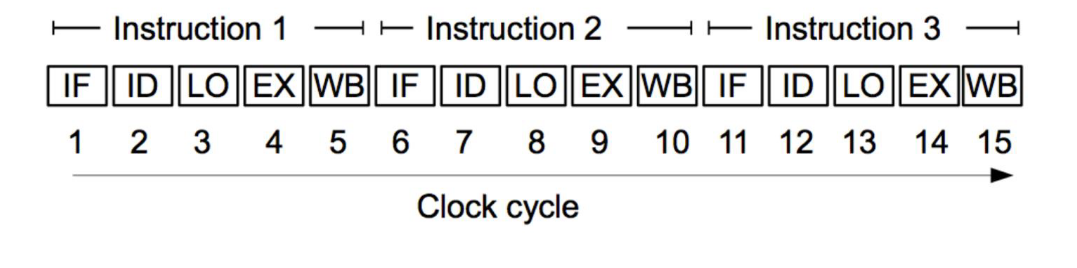
\includegraphics[scale=0.3]{immagini/no-pipeline}
\caption{Istruzioni senza pipeline}
\end{figure}
L'esecuzione in pipeline si basa sulla possibilità di sovrapporre le istruzioni, perché una istruzione non sta usando alcuni componenti della CPU che possono essere usate da altre: ad esempio, se una istruzione è nella fase di ID, di sicuro non starà usando i componenti necessari alla IF, e così valore per un'altra che è nella fase di LO o di EX. La figura in seguito mostra un caso di esecuzione con pipelining 
\begin{figure}[ht!]
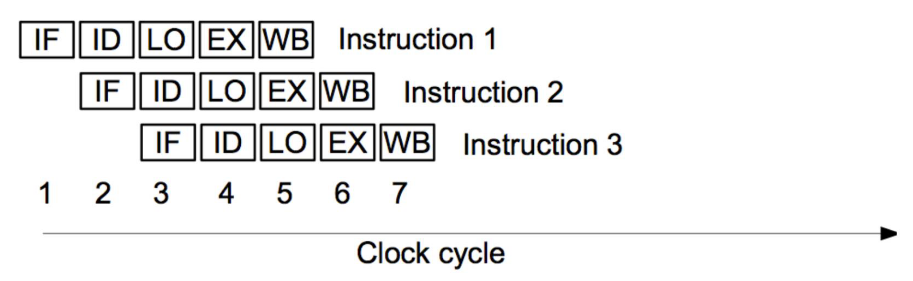
\includegraphics[scale=0.3]{immagini/pipeline}
\caption{Istruzioni con pipeline}
\end{figure}
Questo è l'ILP, e questo tipo di architettura è la base che, con altre tecniche, permettono di eseguire altro per affrontare problemi come il fatto che ogni operazione come la LO richieda più cicli di clock. Non sappiamo a priori quanti cicli di clock richiede una istruzione, quindi il problema va affrontato. Inoltre, l'altro problema è legato ai \textbf{breaks:}se ho un'istruzione di salto e riesco a capire dove saltare solo quando l'istruzione è finalizzata, l'istruzione che viene inserita in seguito a questa potrebbe essere differente da quella da immettere effettivamente e che si saprebbe solo alla fine. Questo è il problema può essere di due tipi:
\begin{itemize}
\item \textbf{control dependency};
\item \textbf{data dependecy}, dove il dato è richiesto da una istruzione in un momento in cui non è disponibile.
\end{itemize} 
\textbf{esempio: analisi di speedup}\\
Supponiamo di voler fornire N risultati, uno per ogni istruzione e di avere L stadi di processamento ed un ciclo di clock di lunghezza T.\\ Senza pipeline, avremo un delay pari a \[ N \cdot L \cdot T\]. Con il pipelining, otteniamo un delay pari a \[(N+L)\cdot T\] dove lo speedup sarebbe dato da \[\frac{N \cdot L}{N+L}\], ovvero circa L per un N grande.\\ Ovviamente, maggiore è L e più il fattore di speedup cresce, ma tipicamente i processori pipelined hanno sui 10 stadi massimo.\\ Ovviamente, abbiamo uno speed up ideale, il problema è che non consideriamo i problemi sopra citati: non è detto che si riesce a committare una istruzione per ogni ciclo di clock, quindi possono essere richiesti molti più cicli di clock. Ampliando la pipeline, si amplia la \textbf{capacità di fare}, quindi inserire nel processore hw per fare operazioni che poi magari non vengono eseguite.
\subsection{Processori moderni}
Gli stage di pipeline non sono molti (ordine delle decine), quindi vediamo cosa è stato adottato per risolvere tutta la serie di problemi visti.\\ Abbiamo, fra le soluzioni possibili:
\begin{itemize}
\item software stall: inseriamo, in un flusso di programma, delle istruzioni di stallo fra due istruzioni. Se ho un salto e non so dove, metto degli stalli finché so se saltare o meno; questo meccanismo è adottato dai compilatori
\item software re-sequencing (o scheduling): anche questo viene fatto dai compilatori, quando si rendono conto che c'è un blocco atomico di programma (ovvero un flusso eseguito nel complesso) si ri-organizza il blocco di istruzioni in modo che istruzioni che si dipendono siano più distanziate
\item per i salti, c'è la branch prediction: se non si sa quale è l'istruzione a cui saltare, si fa una previsione e si fa il fetch di quella zona di codice predetta
\item \textbf{out-of-order pipeline (OOO)}: la base di ciò che accade in una architettura moderna. Importantissimo per permettere alla CPU di essere efficace ed efficiente con generiche sequenze di istruzioni: se una istruzione deve aspettare dei dati, un'altra successiva può andare avanti superandola fino anche completare, \textbf{ma senza rendere visibili le cose nell'ISA}, o si violerebbe il flusso di programma. Quindi, l'OOO non è basato su come le istruzioni toccano l'ISA, ma sul fatto che alcune istruzioni devono aspettare e quindi è possibile far passare avanti a queste le altre.
\end{itemize}
\section{La pipeline nell'x86}
Il processore x86 a 64 bit moderno ha più o meno lo stesso set di registri di un processore di un processore come l'8086 (ed altri), la differenza è che sono un po' di più e sono più grandi.\\ I cambiamenti sono interni, ovvero nel come vengono eseguite le istruzioni: i486 è stato il primo ad adottare una architettura pipeline, che viene riportata in seguito
\begin{figure}[ht!]
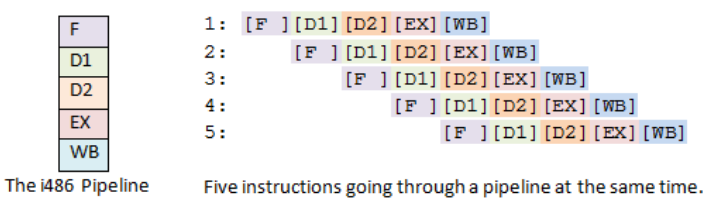
\includegraphics[scale=0.4]{immagini/pipeline-i486}
\caption{Pipeline di i468}
\end{figure}
L'architettura non è "piaciuta" molto, ad esempio se si esegue lo lo XOR fra due registri e si fa per 3 volte consecutive, ognuna delle istruzioni dipende dal risultato precedente in quanto ha una sorgente coincidente con la destinazione, e questo rallentava tutta la pipeline.\\ Se ad esempio, consideriamo del codice C che accede ad un puntatore ed in un caso accede e poi incrementa il puntatore e nell'altro caso accede dopo aver incrementato, questo ha un effetto totalmente diverso. È possibile sperimentare lo stesso problema anche in linguaggi di più alto livello, ad esempio se si incrementa un puntatore:
\begin{itemize}
\item a = *++p
\item a = *p++
\end{itemize}
c'è una differenza in performance evidente fra i due statement. Il file \textit{PIPELINE-TEST/backward-propagation.c}, che gira per 20000 iterazioni, permette di specificare con una macro di compilazione DEPENDENCY se:
\begin{itemize}
\item accedere al puntatore dopo averlo incrementato (e quindi dover dipendere dall'istruzione precedente
\item oppure, se disabilitato, accedere e poi incrementare il puntatore
\end{itemize} 
Se si esegue il programma, si ottengono i seguenti tempi (dipendenti dalla macchina di esecuzione):
\begin{itemize}
\item con dipendenza, si ottiene un tempo di 5.25 secondi
\item senza invece, il tempo è di 5.31 secondi
\end{itemize}
C'è inoltre il problema di istruzioni che causano lo squash della pipeline, ovvero la cancellazione di tutto ciò che vi è contenuto in quel momento. Tali istruzioni possono essere denotate come danno nel nostro programma, in quanto è possibile che vada rifatto tutto il lavoro perso delle successive istruzioni. Se consideriamo x86, una istruzione di questo tipo è \textsf{CPUID}, che prende l'ID numerico del processore su cui si sta lavorando. Questo è fondamentale quando si scrive del sw per il kernel, specialmente quando si sta scrivendo del sw che tocca delle strutture dati per lo specifico processore: bisogna conoscere quale è il processore su cui si lavora.\\ Tali istruzioni sono dette \textbf{serializing}, se però leggiamo il manuale dell'istruzione CPUID ci dice che è garantito che tutto ciò che viene è stato fatto da istruzioni precedenti è stato completato prima che la prossima istruzione sia fetchata ed eseguta.
\subsection{Intel x86 superscalar pipeline}
Per poter superare il problema degli effetti del sw all'interno dell'esecuzione in pipelining è necessario avere una  pipeline avanzata, in modo da poter capire cosa è possibile eseguire in parallelo: questo ha portato allo sviluppo delle \textbf{superscalar pipeline}.\\  Tale pipeline è fatta in modo che in ogni fase c'è più di un componente, ad esempio più componenti di esecuzione, più ALU, che possono essere identici e permettere quindi che l'istruzione possa andare in uno di essi. Se ad esempio l'istruzione richiede l'engine per più cicli di clock, non blocca successive istruzioni che magari poi richiedono lo stesso componente in quanto tale componente è ridondato. C'è quindi parallelismo nella pipepline stessa, inoltre siccome le istruzioni più lente, e che quindi richiedono più cicli di clock, sono un problema, i processori hanno adottato il modello dell'out-of-ordering: se qualche istruzione è ferma, le altre vanno avanti rispettando comunque il data flow model.\\ Tali aspetti erano nati molto prima, ad esempio nell'IBM 360/91 degli anni 60', si parlava però di architetture particolari ed il tutto preveda che nella pipeline ci fossero altri componenti per gestire l'OOO.\\ Le basi del progetto erano:
\begin{itemize}
\item come mettere in commit le istruzioni in program order: fare uscire una istruzione dalla pipe indica che l'effetto dell'istruzione sulle risorse dell'ISA divine visibile, quindi è delicato capire quando mandare in commit
\item processare istruzioni indipendenti, sia sui dati che sulle risorse, il prima possibile
\end{itemize}
Vediamo come affrontare il problema che ogni istruzione possa durare un certo numero di cicli di clock
\subsubsection{Istruction span problem}
Ogni istruzione può durare un certo numero di cicli di clock, a seconda di cosa deve fare e per effetti diversi, ad esempio può essere necessario attendere componenti esterni alla CPU come la memoria. Il fetch dei dati può portare via diversi cicli di clock, e si è cercato di risolvere questo come problema centrale con le pipeline super-scalari.\\ Con una OOO pipeline, può accadere la seguente cosa\\\\
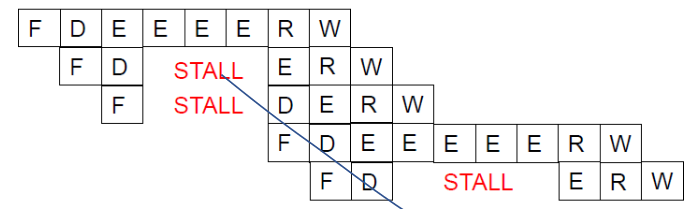
\includegraphics[scale=0.5]{immagini/ooo-pipeline-1}\\
la seconda istruzione può avere uno stallo, magari perché non ha i dati. Come vediamo, in realtà l'istruzione ha bisogno di un solo ciclo di clock di esecuzione, ma ne usa di più perché non ha i dati disponibili. Anche la 3° istruzione è bloccata e lo stesso vale per l'ultima, perché deve usare lo stesso componente. Ricordiamo che il delay può avvenire perché il componente da usare non è pronto.\\ In OOO accade la seguente cosa: lo stallo diviene un ri-ordinamento\\\\
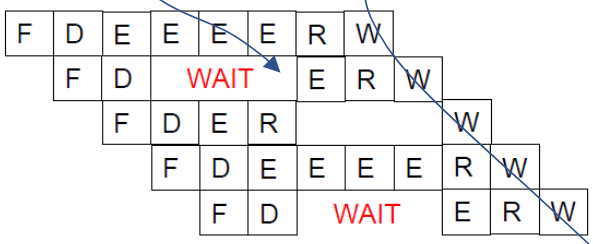
\includegraphics[scale=0.5]{immagini/ooo-pipeline-2}\\
può accadere che istruzione 1 e 2 usino due componenti identici nella pipeline, e che la 3° entri in esecuzione ed abbia pronto il risultato molti cicli di clock prima di quando serve, quindi occorre mantenerla uncommitted e metterla in write back solo in maniera coordinata. Ad ogni ciclo di clock è possibile mandare in commitment il lavoro anticipato: se riusciamo a far entrare una istruzione ogni ciclo di clock, riusciamo a farne uscire una ogni ciclo di clock, avendo lo stesso throughput in ingesso ed in uscita rispetto alla pipeline tradizionale.
\subsection{Pipeline OOO speculativa}
Quando si parla di pipeline OOO, si parla anche di pipeline speculative: su un flusso di programma, se processiamo una istruzione successiva rispetto ad una che deve ancora essere processata, stiamo dicendo che c'è indipendenza fra le due, ma questo non è sempre vero. Quello che è in pipeline sta in realtà eseguendo in maniera \textbf{speculativa}, si fa fetch di una istruzione successiva e poi magari le istruzioni non verranno eseguite perché si salta altrove. Inoltre, una istruzione in qualunque ciclo di clock può generare una \textbf{trap}: si potrebbe consultare il TLB (caching), ci rendiamo conto che qualcosa non va e quindi l'istruzione non può essere mandata in commit. Se c'è una trap mentre un program flow esegue, va passato il controllo ad un gestore lato sw, quindi tutte le istruzioni che venivano eseguite dopo erano eseguite in maniera speculativa e non andranno mai a commit point.\\ Distinguiamo fra due concetti:
\begin{itemize}
\item il \textbf{retire} è l'azione del committare una istruzione e rendere i suoi side effects "visibili" in termini di ISA;
\item l'\textbf{emissione} è l'azione di iniettare le istruzioni nella pipeline.
\end{itemize}
Fra le due azioni è possibile che ci siano altre istruzioni di mezzo, ci sono poi anche le eccezioni che vanno gestite correttamente: se una istruzione successiva entrata in pipeline e genera una eccezione, ha senso eseguire un cambio di flusso per gestire l'evento particolare? No, in quanto l'istruzione è eseguita in modo speculativo e quindi finché non arriva alla fase di write back può scomparire dal flusso, perché anche le istruzioni precedenti sono speculative e magari una istruzione precedente genera l'eccezione che rende l'eccezione di quella successiva inutile, perché l'istruzione non doveva proprio essere nel flusso di programma.\\ Quindi le eccezioni sono imprecise, non è detto che quando vengono generate queste esistano o meno, saranno effettive solo se le istruzioni arriveranno al commit point.\\ Inoltre, l'eccezione viene generata considerando che in parallelo stiamo facendo altro in una OOO pipeline:
\begin{itemize}
\item una istruzione precedente è stata superata
\item una istruzione successiva ha superato
\end{itemize}
quindi quando viene generata la trap, lo stato effettivo del processore e di conseguenza quello di tutti i componenti non esposti nell'ISA globalmente può essere stato cambiato in modo parziale da istruzioni che precedevano quella che ha generato la trap, ma anche da istruzioni successive. Quindi, come implicazione importante, tutte queste istruzioni possono generare dei side effect che possono essere sfruttati per attaccare le applicazioni ed i sistemi, prelevare dati a cui non si può accedere etc...\\ Di seguito, viene mostrato uno schema esemplificativo della pipeline OOO\\\\
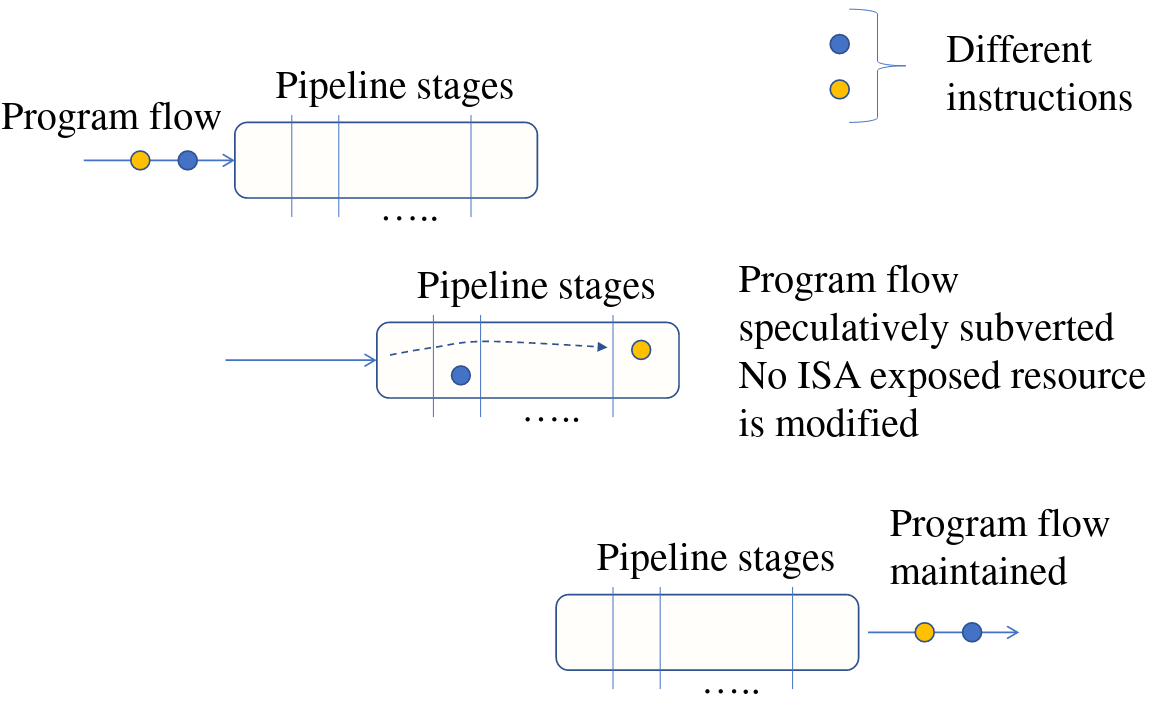
\includegraphics[scale=0.2]{immagini/pipeline-ooo}\\
come mostrato nell'esempio, può accadere che l'istruzione gialla arrivi a commit point prima  di quella blu e questo permette di portare a termine lavoro utile anche quando altre istruzioni sono bloccate per i vari motivi detti prima.
\subsubsection{Eccezioni imprecise}
Su una architettura pipeline OOO (ma anche generale) in cui le istruzioni si superano l'un l'altra con un ILP molto elevato, consideriamo che una istruzione A è dopo una B nel program flow e B che causa una eccezione. Quindi, B $\rightarrow$ A (B precede A) ed A entra in pipeline prima di B, ma se B ha una eccezione, possono esserci tante altre istruzioni successive che l'hanno superata dopo A in pipeline e queste possono aver cambiato molto nello stato della CPU, tutte le relazioni di dipendenza possono essere state portate avanti in maniera speculativa senza toccare i registri di CPU, ma toccando altri elementi. Può accadere che ci siano anche altre relazioni, ad esempio B genera dei valori che poi verranno usati da A e che A poi passi il risultato basato su tali valori ad altre istruzioni dopo di lei etc... \\ Si toccano componenti nella CPU in funzione del fatto che vengono anche passate informazioni in maniera speculativa e non a livello dell'ISA. Questa è stata la base dell'attacco \textbf{meltdown}, in cui è stata necessaria la patch di tutti i kernel esistenti: è possibile usare i processori OOO per leggere dati del kernel, è possibile leggere buffer cache e quindi leggere i file o i meta-dati per proteggere i dati (ad esempio dati di cifratura).
\\ Quindi, se siamo in pipeline occorre stare attenti, altrimenti si scrive software di sistema non corretto. Può accadere che viene passato un output in maniera speculativa e che ci siano effetti su altri componenti della CPU. \\ Considerando lo schema seguente:
\begin{figure}[!ht]
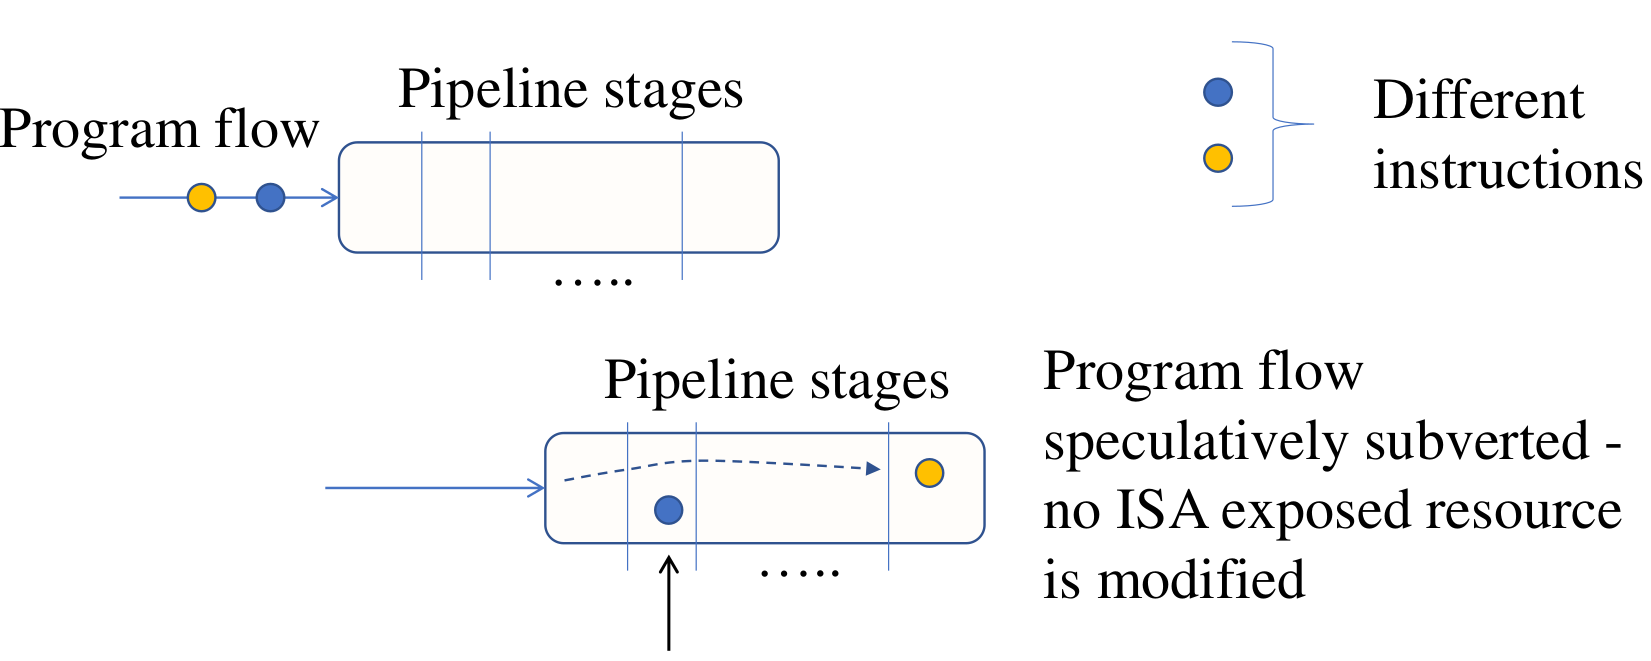
\includegraphics[scale=0.15]{immagini/not_valid_instr}
\end{figure}
Se l'istruzione accede a delle risorse non valide, come locazioni di memoria o componenti della CPU non accessibili temporaneamente, il flusso di programma non è più valido e quindi anche le altre istruzioni non sono valide, ma possono esserci dei side effect nell'hardware dovuti al fatto che tali istruzioni sono già state processate
\subsection{Algoritmo di Robert Tomaluso}
Le architetture moderne hanno delle varianti rispetto a questi algoritmi. Consideriamo come avviene il passaggio fra due istruzioni A e B per cui A$\rightarrow$B nel program flow, le possibili dipendenze sono:
\begin{itemize}
\item RAW (Read After Write): B legge un dato prima che A lo scriva, il che porta ad uno stallo e quindi c'è una dipendenza sui dati
\item WAW (Write After Write): B scrive un dato prima che A scriva lo stesso dato. Anche qui abbiamo una dipendenza sui dati
\item WAR (Write After Read): B scrive un dato prima che A legga lo stesso dato, quindi il dato letto non è consistente.
\end{itemize}
Come risolviamo queste dipendenze sui dati: Tomasulo propone delle idee algoritmiche per un processore OOO:
\begin{itemize}
\item RAW: per ciascuna lettura, bisogna tenere conto se il valore da leggere è già stato prodotto, l'attesa del dato va quindi inserita nella OOO e quindi nel caso sia necessario bisogna considerare il buffering dell'operazione;
\item WAR e WAW: la soluzione adottata è quella dei \textbf{renamed registers}. 
\subsubsection{Renamed registers}
Supponiamo di avere un registro R, per gestire WAW facciamo si che i due valori siano scritti ma sue due registri diversi. R non è un singolo registro, bensì è un \textbf{multi-registro}, dove ci sono varie versioni del dato. Qualsiasi istruzione che deve scrivere un valore in un registro ed entra in pipeline va sul componente, preleva uno slot utilizzabile fra i molti che compongono il multi-registro e scrive il valore in quello slot. Quindi, nel program flow può accadere che i valori possono essere scritti in tempi differenti sullo stesso registro, ma grazie alla presenza degli slot si risolve WAW, in quanto in termini di commit del valore verrà ristabilito l'ordine corretto. Il valore non può sovrascrivere, perché viene scritto su uno slot, quando viene mandata in commit l'istruzione si avrà il valore effettivo associato al registro R, nel controller del registro c'è anche quale è la versione attuale del valore del registro.\\ Un solo valore alla volta è quello attivo, alcune versioni saranno del passato ed altre del futuro, nella storia dei commit che poi verrà realizzata.\\\\
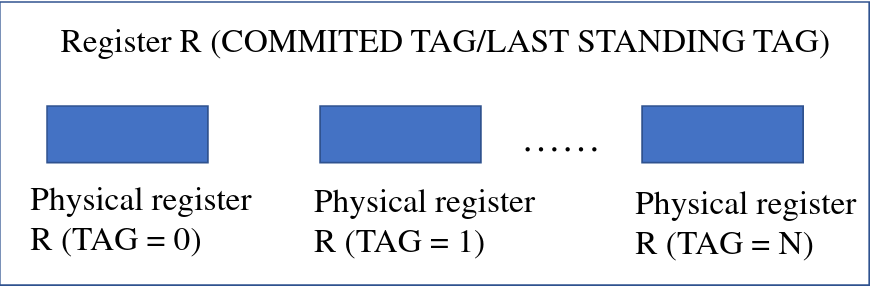
\includegraphics[scale=0.25]{immagini/multi-registri}\\
Quindi, quando mandiamo in pipeline una istruzione che deve leggere R, la marchiamo con il valore che quella deve leggere e finché il registro non è pronto l'istruzione rimane bloccata. Tutto questo è invisibile al programmatore in termini di risorsa ISA, ma visibile in termini del fatto che è possibile far si che il software faccia cambiare stato a tutti i registri in modo da creare problematiche.\\ In maniera indiretta è stato risolto anche WAR: per WAW è stato risolto il problema utilizzando i tag, ma anche per WAR finché il tag da leggere non è pronto, l'istruzione rimane ferma
\end{itemize}
\subsubsection{Reservation stations}
Ogni istruzione ha un codice operativo, che va bufferizzato da qualche parte e poi va relazionato al componente che deve eseguire l'operazione. La reservation station è una zona del processore che svolge tale funzionalità di buffer, in cui viene registrata una operazione in input all'oggetto (elemento operativo dell'hardware) che può eseguire quella operazione, ad esempio somme etc...\\  Non è detto che l'operazione venga processata immediatamente, perché può essere coinvolta in una dipendenza e dover attendere dei dati non ancora prodotti, questo viene dettato dallo stato del renamed register. La reservation station permette la possibilità di riservare il componente per l'istruzione, finché quest'ultima non è pronta ad essere eseguita.\\ Le reseravtion stations contengono:
\begin{itemize}
\item OP - l'operazione da eseguire (ovvero il codice);
\item $Q_j, Q_k$ - le reservation stations che produrranno l'input necessario ad OP;
\item in alternativa a $Q_j, Q_k$ ci sono $V_j, V_k$ ovvero i valori attuali (ad esempio i valori di registro) da usare come input per OPs
\end{itemize}
I registri, d'altra parte, sono marcati con la reservation station Q tale che produrrà il nuovo valore da scrivervi, se ce n'è bisogno.
\subsubsection{CDB e ROB}
Supponiamo di avere una reservation station in cui ci sia una operazione in coda: il flusso di informazioni fra le componenti deve essere supportato, che avviene usando il \textbf{Common Data Bus}, che permette di spostarle fra i vari componenti per garantire il corretto flusso di input fra le varie istruzioni.\\ Il \textbf{ReOrder Buffer} mantiene invece i meta-dati delle istruzioni non ancora committate, in quanto bisogna ricordarsi quale è l'ordine logico con cui andarle a committare, e questo tiene conto dell'ordine. Inoltre il ROB acquisisce tutti i nuovi valori prodotti dalle istruzioni (anche quelli che transitano nel CDB), mantenendoli uncommitted fino a che l'istruzione non viene ritirata. Questo mantenimento può essere fatto direttamente oppure referenziando l'alias di registro che deve mantenere tale valore.\\ Il ROB è anche usato per gli input delle istruzioni che necessitano di leggere valori non committati.
\subsubsection{Schema architetturale}
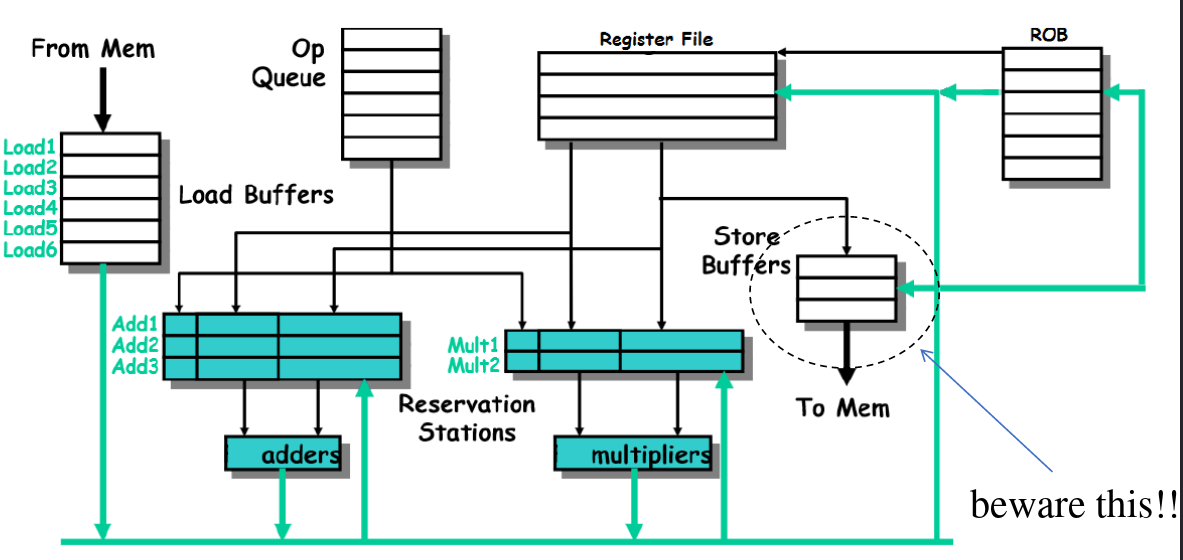
\includegraphics[scale=0.25]{immagini/arch-moderna}\\
Lo store buffer è un altro componente interessante: è fondamentale per interagire con la memoria. Mantiene in maniera temporanea il valore da scrivere per i dati verso la memoria. Lo SB viene toccato solo quando viene committata una istruzione, ed il valore viene scritto nello SB, non in memoria: in una architettura OOO quindi non si ottimizza solo il pipelining, ma anche la scrittura verso la memoria, perché se dovessimo scrivere in memoria a commit-time, la entry del ROB sarebbe occupata per vari cicli di clock e verrebbero bloccati diversi componenti senza poter andare avanti. Dallo SB i valori possono anche essere letti, e finché il valore non viene riportano in memoria è visto solo dal singolo program flow, magari perché questo necessita di ri-accedervi diverse volte durante l'esecuzione. Da qui scaturisce il problema della sequential consistency, dove se qualcuno produce qualcosa questo non è visibile ad altri.\\\\ \textbf{esempio:} abbiamo 3 istruzioni che entrano in pipeline, con i rispettivi delay $\delta$ per essere processate.
\\\\
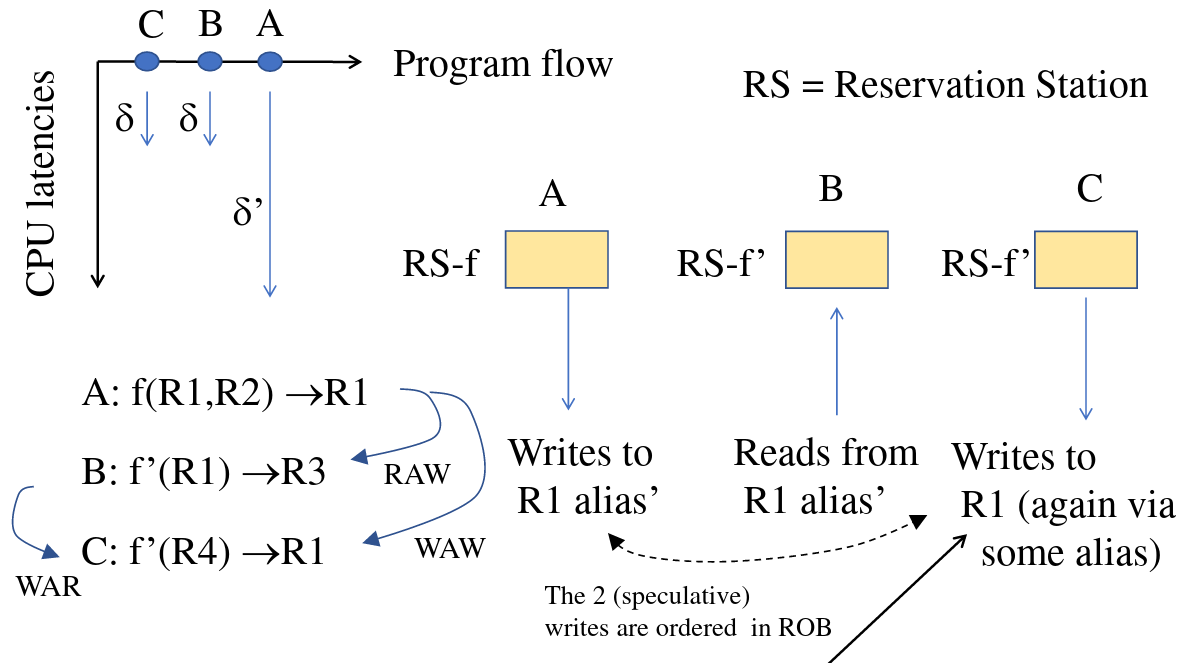
\includegraphics[scale=0.25]{immagini/ex-pipeline}
\newpage
Di seguito invece, viene mostrato un esempio che lega il ROB all'esecuzione delle istruzioni\\
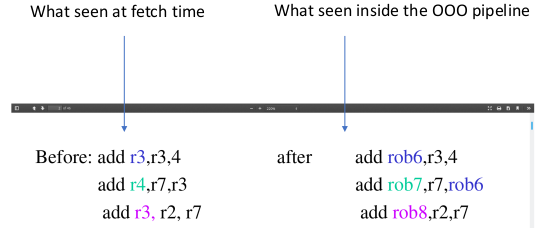
\includegraphics[scale=0.6]{immagini/rob}
\subsubsection{Storia}
Nell'architettura basata sull'algoritmo di Tomasulo, storicamente, venivano mandate out of order solo determinate istruzioni, mentre nei processori moderni l'OOO è visibile su tutto l'insieme delle istruzioni. Nell'evoluzione storica c'erano solo istruzioni in floating point, oggi si copre tutto il set di istruzioni
\subsection{Ancora sul memory wall}
Nel tempo, la memoria ha accelerato nella capacità di fornire informazioni, ma i processori hanno accelerato ancora di più nella richiesta delle chiamate a memoria. Quindi, guardando le 3 istruzioni precedenti ed i delay, ci sono anche i delay dovuti alla latenza per i miss in cache. Come vedremo, questo è stato il motivo della nascita delle architetture hyper-threading, ovvero la divergenza fra i due mondi.
\subsection{OOO nell'x86}
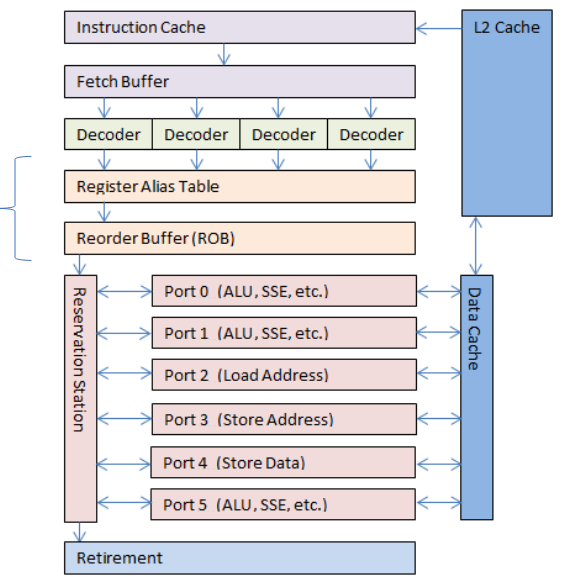
\includegraphics[scale=0.3]{immagini/x86-ooo}\\\\
A livello alto, nell'x86 abbiamo la Register Alias Table, il Reorder Buffer e tutta una serie di hardware replicato. Quando un oggetto entra nel Reorded Buffer, il firmware sceglie uno o l'altro componente replicato e ci sono poi le diverse relazioni che esistono fra i diversi componenti.\\ Questo fa capire che vengono caricate più le istruzioni alla volta, difatti viene caricata una intera linea di cache che in x86 è da 64 byte, in cui si possono mettere diverse istruzioni: alcune andranno in commit ed altre no, però ci sono molte cose che si passano informazioni e fanno attività.\\ L'OOO ha permesso di fare le operazioni talmente tanto velocemente che il core engine non veniva usato a pieno, anche per colpa delle latenze dovute agli accessi in memoria. Quindi, la questione posta fu quella di utilizzare lo stesso engine per molteplici flussi di programma, ovvero si introdusse \textbf{l'hyper-threading}, esposto al programmatore ad ogni livello, sia user che OS etc...\\ I registri esposti dall'ISA sono replicati, come se ci fossero due processori distinti, ma nel complesso l'OOO non viene esposto al programmatore, anche se il modo di scrivere il software può impattare l'efficacia dell'OOO stesso e, più in generale, il pipelining.
\subsubsection{Hyper-threading}
La necessità della nascita delle architetture hyper-threading è nata perché la struttura della CPU era talmente ottimizzata da rimanere senza fare nulla per troppo tempo, non riusciva più ad essere fillato in maniera efficiente quando i dati dovevano salire in memoria.\\ Le architetture ad hyper-thread prevedono che, siccome il "motore" è così rapido ed efficiente, si mandano due linee di input in parallelo, che sono due processori effettivi su un unico core: due program flow diversi su i due processori. Quando poi le istruzioni sono processate, si usa l'unico engine: il classico è avere 2-1 (es: 8 thread, 4 core). C'è una buona replicazione dei componenti, per evitare che se un flusso insista su un componente in particolare, non ci sia blocco.\\ Un altro aspetto importante è la sicurezza: se c'è un interferenza fra i due thread in esecuzione che prevede che si vedano dati di uno dall'altro, bisogna "spegnere" uno dei due e sfruttare meno potenza effettiva.
\\\\
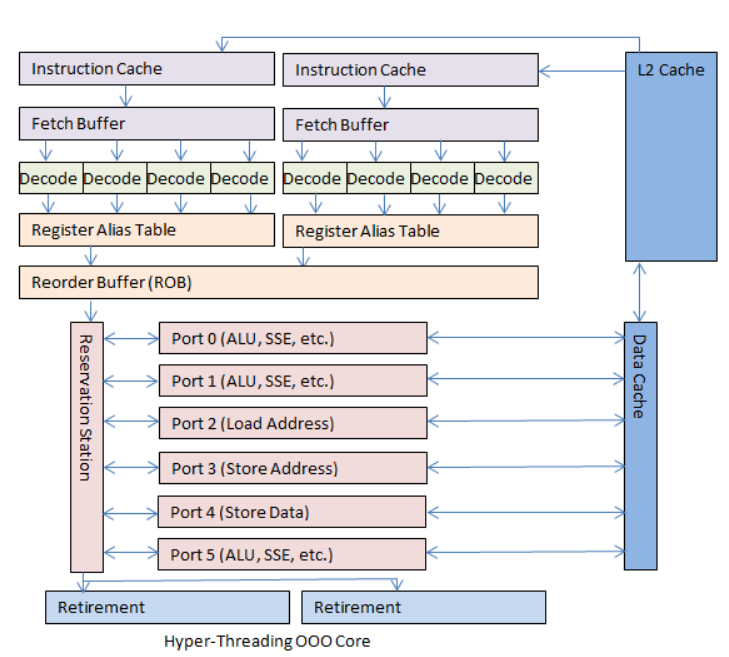
\includegraphics[scale=0.3]{immagini/hypert-ooo}\\
In questa architettura ci sono due hyper-thread ed una sola architettura per processare le istruzioni dei flussi e non c'è interferenza fra i due flussi, quindi quando l'istruzione scrive su un registro la risorsa è accessibile solo da quel flusso, ma la scrittura è tale per cui i componenti siano utilizzati per le istruzioni anche dell'altro flusso ma queste vengono usate in time sharing: gli oggetti non sono esposti nell'ISA, quindi questo non crea problemi a cosa è scritto nei programmi. In ogni caso, ci sono dei side effects sugli engine quando si esegue in hyper-threading, che sono problematici per la sicurezza.
\subsection{Gestione degli interrupt}
Ogni sistema moderno è interrupt-driven, quando c'è un interrupt bisogna eseguire una porzione di codice per rispondere agli interrupt.\\ Quando siamo sulla pipeline, avere un interrupt significa dire che siamo entrati con una serie di istruzioni sul thread corrente e l'interrupt vuole che si passi a prelevare istruzioni da un'altra zona di memoria, l'interrupt si accetta sempre quando una istruzione ha completato (per evitare di dover salvare lo stato dell'istruzione corrente). Per le altre istruzioni, che magari hanno già eseguito in maniera speculativa: 
\begin{itemize}
\item o si salva lo stato della pipeline;
\item oppure (più comodo) viene fatto lo squash della pipeline e si comincia a ri-fillare con le nuove istruzioni la pipeline
\end{itemize}
Questo ci fa capire che nei processori moderni l'interrupt costa: si butta del lavoro fatto e quasi finalizzato perché va squashato il contenuto nella pipeline, e quindi anche i valori scritti speculativamente negli alias dei registri, teniamo però bene in mente che le istruzioni in esecuzione e non completate e che vengono squashate possono aver cambiato lo stato micro-architetturale della macchina.\\ Ci saranno delle policy per distribuire questa cosa su tutti i core presenti nell'architettura.
\subsection{Trap e stadi della pipeline}
La trap è qualcosa di sincrono rispetto all'interrupt che è asincrono, capita perché il programma sta facendo qualcosa. Su una architettura pipeline, possono essere generate le seguenti trap in generali:
\begin{itemize}
\item Instruction Fetch \& Memory stages: l'istruzione può essere offending, quindi non è possibile finalizzarla per via di:
\begin{itemize}
\item Page fault, ovvero l'indirizzo di memoria logico a cui accediamo non sappiamo a cosa corrisponda;
\item Accesso in memoria misaligned, ovvero ci sono istruzioni che per lavorare correttamente hanno bisogno di indirizzi di memoria allineate ad una certa potenza di 2. 
\item Memory-protection violation, ad esempio scrivere su una pagina read only: tale informazione viene data dalla page table e cachata nel TLB
\end{itemize}
\item Instruction decode stage: operazione illegale, un program counter ha detto lungo un program flow di prelevare l'istruzione ed eseguirla nel processore ma questa non è eseguibile dal processore. 
\item Execution stage: possono esserci problemi sull'esecuzione vera e propria, ad esempio divisione per 0, quindi eccezioni aritmetiche
\item Write back: non ci sono eccezioni tipicamente
\end{itemize}
Per una certa istruzione, è possibile subito accorgersi se questa sia offending e quando viene identificata come tale, nel momento in cui entra in pipeline e non l'ha ancora attraversata, cosa si fa? Si butta tutto il lavoro in pipeline? No, perché questa potrebbe aver superato altre istruzioni e quindi sta eseguendo in maniera speculativa, per cui si rischierebbe di buttare cose che vanno finalizzate. Come ci si comporta: si può far cambiare il flusso all'interno della pipeline, eseguendo attività differenti nel momento in cui l'istruzione non fosse offending ed altre attività se lo fosse.\\ Oppure è meglio marcarla con un bit ad 1, in modo da ricordarsi che è offending e quando arriva a commit point, la mando in abort e possono mandare in abort tutto il resto perché a quel punto tutto quello che era precedente è andato in commit.\\ Perché la scelta migliore è la 2, ed è stata applicata nell'architettura di processore: quando un'istruzione attraversa una pipeline, viene gestita da un micro-codice, ovvero un sotto-sistema di controllo che sa cosa fare per ogni tipo di istruzione. Per gestirla in maniera adeguata, dovrei avere un micro-codice apposito per gestire una istruzione offending in un certo punto, quindi questo comporterebbe una complessità maggiore nel micro-codice per la gestione delle istruzioni. Quindi si evitano transistor per introdurre ulteriore logica, risparmiando spazio per ampliare l'hardware per fare delle operazioni più utili.\\ Quindi si aggiunge un bit ad 1 per indicare che l'istruzione è offending, ma questo vuol dire che tutti gli altri passi dell'istruzione vengono portati avanti: tutto quello che si fa per quella istruzione è tale per cui tutto quello che l'istruzione sta facendo non era permesso. Ma se ho un memory access violation, l'istruzione nella pipeline può aver passato in un alias di registro le informazioni lette nel caso della violazione e può essere letta da una istruzione successiva, questo crea una serie di side effect: A accede a dei dati non permessi, li passa a B ed etc... i side effects generabili sono funzione dei dati acceduti e questo è un problema.\\ Questo è l'attacco meltdown
\subsection{Meltdown attack}
Supponiamo di avere a disposizione un flusso di istruzioni in esecuzione in un'area di memoria, dove abbiamo un array di 256 byte. Supponiamo di avere un byte in un altra locazione di memoria: possiamo scrivere un programma che usa questo byte come offset nell'array (essendo 256 possibili valori, riusciamo ad indicizzare tutto l'array), accedendo quindi ad I[c]. Cosa è successo nell'architettura quando facciamo I[c]: abbiamo caricato c in memoria nel registro R ed usato R per accedere ad I. L'operazione di caricare c nel registro è in una architettura vera:
\begin{itemize}
\item può essere un'operazione speculativa, così come l'accesso in memoria usando il valore caricato di c
\item nell'architettura quello che accade e che un'istruzione ha chiesto di prendere c e metterlo in un registro. C'è un RAM per farlo fluire in un registro, c deve salire nell'architettura e passare per la cache. Quindi la lettura di c da usare come indice fa si che c passi comunque per la cache in una architettura moderna. Anche I[c] passa per la cache, se qualche istruzione vuole leggere questo byte deve passare anche lui per la cache.
\end{itemize}
Magari le due istruzioni sono offending, magari c è un valore inaccessibile al flusso di programma che è user-level e c è in zona kernel. L'istruzione va comunque avanti, con anche quelle successive, ma la cache ha cambiato stato. Quello che ha cambiato stato della cache è il fatto che uno dei caratteri è salito in cache, l'array potrebbe essere lecito perché magari è applicativo ed il che vuol dire che è stato creato un side effect per cui un suo byte è stato caricato in cache. Si può ri-accedere all'array dopo aver eseguito questa istruzione? Si, eseguendo una funzione di gestione del segmentation fault e posso capire se dato un array di valori alcuni sono in cache ed altri no: basta leggerli e misurare il tempo di accesso al valore per distinguere fra cache hit ed cache miss. Quello in cache sarà esattamente in posizione c e quindi posso dedurre il valore di c, che può essere un byte kernel sapce che non avrei dovuto leggere.\\ Riassumendo il funzionamento di meltdown:
\begin{enumerate}
\item facendo cache flush, fattibile a livello user. Possiamo limitarlo anche solo all'array desiderato
\item leggiamo un byte B di livello kernel
\item usiamo il byte B per leggere una zona di memoria lecita, quindi in questo caso l'array detto prima
\item L'istruzione intermedia è offending, la zona successiva è phantom perché non esisterà in quanto non andrà in commit, ma possiamo vedere se ci sono stati dei side effects.
\end{enumerate} 
L'array della cache non è di caratteri, ma è di pagine: una cache line porta vari byte, un minimo di 64 su x86 ma anche il doppio o il triplo, quindi se leggo un byte l'architettura ne porta in cache parecchi di più. Quindi il byte non va bene come unità di misura, non possiamo discriminare quale è il valore di c da inferire.\\ Le pagine sono di 4096 byte, e sono 256 pagine, usiamo c per accedere al 0-esimo byte della pagina, per cui c identifica la pagina a cui ho acceduto. Se la pagina non è in cache assolutamente, non era in cache, se invece il byte 0 c'è ed è seguito da altri allora c identifica la pagina.\\ Nella demo ci sono due comandi cat del file /proc/nome\_file perché così facendo, chiedendo al kernel il dato e scrivendolo altrove, i cat portano in cache i dati del segreto che sto cercando di scoprire e quindi velocizzano nell'operazione di retrieve che si cerca di eseguire.
\paragraph{Side channel:}per portare a termine il meltdown, si usa un side channel. All'interno dell'esecuzione è possibile generare dei cambi di stato che non sono visibili nell'ISA, perché non esistono istruzioni per leggere il dato direttamente dalla cache, ma che possono essere osservati in altro modo. Alla base di tutti gli attacchi su macchine moderne ci sono i side channel
\subsection{Dettagli di x86 64 bit - Instruction Set}
In x86 ci sono 16 registri general purpose a 64 bit, ma è retro compatibile con la versione a 32 bit in cui c'erano solo 8 registri a 32 bit.\\ I registri originali a 32 bit avevano determinati nomi ed è possibile utilizzarli ancora mediante il nome, per prendere i 32 bit meno significati del registro. Anche in un registro a 32 bit si possono gestire la metà del registro ed il singolo byte, lavorando a grana più fine, stesso vale per l'instruction pointer.\\ Ci sono poi altri registri per processare delle istruzioni particolari, che sono a 128 bit e poi dei registri per le istruzioni floating point.\\ Le istruzioni sono abbastanza e semplici similari:
\begin{itemize}
\item \textsf{mov\{b, w, l\}} (se byte, word o longword) \textsf{source dest}. Se non si specifica la size, la mov lavora a 64 byte
\item \textsf{push\{w, l\} source}
\item \textsf{pop\{w, l\} dest}
\end{itemize}
Per costruire un indirizzo per accedere alla memoria si può fare o con un indirizzo assoluto oppure specificando un offset all'interno dell'address space. In generale un indirizzo su x86 può essere targato con
\begin{itemize}
\item displacement, a questo possono essere sommati altri punti
\item base: può contenere un puntatore per accedere alla memoria
\item index + scale: altro offset che si può aggiungere ed è funzione di un pointer moltiplicato per un certo valore 
\end{itemize}
La figura di seguito riassume i possibili addressing:\\\\
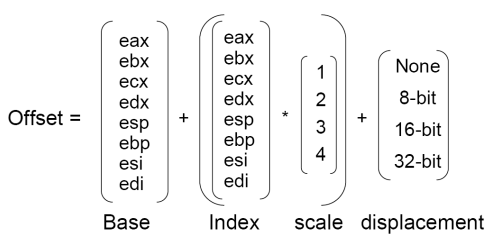
\includegraphics[scale=0.6]{immagini/address_offset}\\\\
È quindi possibile avere i seguenti casi:
\begin{itemize}
\item solo displacement: \textsf{movl foo, \%eax};
\item solo base: \textsf{movl (\%eax), \%ebx};
\item base + displacement: \textsf{movl foo(\%eax), \%ebx};
\item (index * scale) + displacement: \textsf{movl (,\%eax,4), \%ebx};
\item base + (index * scale)+displacement: \textsf{movl foo(\%ecx, \%eax, 4), \%ebx};
\end{itemize}
Ci sono anche gli operatori logici ed istruzioni aritmetiche.
\subsubsection{Meltdown in assembly}
La sintassi intel prevede di usare prima il registro dest e poi src
\begin{lstlisting}
; rcx = kernel address
; rbx = probe array

retry:
mov al, byte [rxc]
shl rax, 0xc
jz retry
mov rbx, qword [rbx+rax]
\end{lstlisting}
l'array è fatto di pagine di 4096 byte, quindi lo shift del contatore letto all'indirizzo kernel va fatto per indicizzare le diverse pagine, shiftando di 4096. Il valore trovato in rax può essere 0 se ho letto il valore 0, quindi salto su retry per rileggere lo stesso byte. Se accedo all'array, andrei nella pagina 0-esima e il valore 0 non è interessante perché è terminatore di stringa. Quindi aspetto che nella concorrenza qualcuno modifichi il valore letto. A quel punto, se non ho letto 0 carico in un altro registro quello che ho letto.\\ Speculativamente ha senso che tutto venga eseguito e che ci siano i side effects sulla cache, ma da un punto di vista reale non ha senso che venga eseguito.
\subsection{Contromisure per meltdown}
Per cercare di ovviare a queste problematiche di sicurezza dovute a meltdown:
\begin{itemize}
\item KASRL: Kernel Address Space Randomization, fa si che quando gira un applicazione, questa non sappia dove il kernel mantiene informazioni nella zona dell'address space. Se non sappiamo dove è mantenuta la chiave nell'address space del kernel bisogna andare verso attacchi bruteforce.\\ Il kernel, quando viene compilato, è pensato per avere le strutture dati e gli indirizzo a partire da una base nota. Con la randomizzazione, il kernel ad ogni statup si ricolloca a partire dalla zona nota, quindi è shiftata di un numero di posizioni che non conosciamo. Questo è possibile solo se gli accessi ai dati ed alle istruzioni in base al displacement avviene in base alla posizione relativa dall'istruction pointer.
\item KAISER, Kernel Isolation
\item Explicity cache flush ad ogni ritorno dal kernel mode: quindi se un flusso riprende il controllo dopo essere stato in kernel mode, si manda la cache in flushing. Ma possiamo avere una applicazione che, nell'asse temporale esegue come user, poi come kernel, poi di nuovo user etc... Se si fa questo la cache sta venendo buttata, quindi è come non averla in quanto viene sprecata in maniera sostanziale. Inoltre, ci sono anche attacchi che non passano per karnel.\\ La protezione può essere utile anche in un altro scenario: user eseguite in maniera malevola, quindi ci sono dei side effects che verranno osservati dopo. È possibile avere un percorso di questo tipo: eseguo, passo al kernel, il kernel esegue e mi rida il controllo. Se non valesse questa cosa, io saprei che le sys call che chiama il kernel durante quella esecuzione porta in cache dei dati che voglio attaccare. Quindi, potrei avere un attacco subito dopo la syscall.
\end{itemize}
La soluzione utilizzata ad oggi è KAISER, che sfrutta questa cosa: abbiamo analizzato le trap che possono capitare all'interno dell'attacco meltdown ovvero le memory protection violation. KAISER è tale per cui non è possibile generare quella trap per accedere a delle informazioni di zona kernel. In particolare, la page table per il programma ha le entry che afferiscono alla zona di address space user settate, mentre quelle che afferiscono alla zona kernel non sono settate e quindi generano trap di tipo page fault.\\ Ma è possibile avere una applicazione che quando esegue ha solo come pagine valide nella PT relative allo user space? No, è ideale: nell'address space, il kernel è visibile tramite la PT, il kernel non è reso tutto invisibile ma sono una zona. La zona visibile è l'unica usabile per entrare ed eseguire in modo kernel, una volta entrati si cambia la visibilità anche sul resto della zona. Quindi, in user space non si può accedere alle zone invisibili. L'implementazione attuale è la seguente: \\
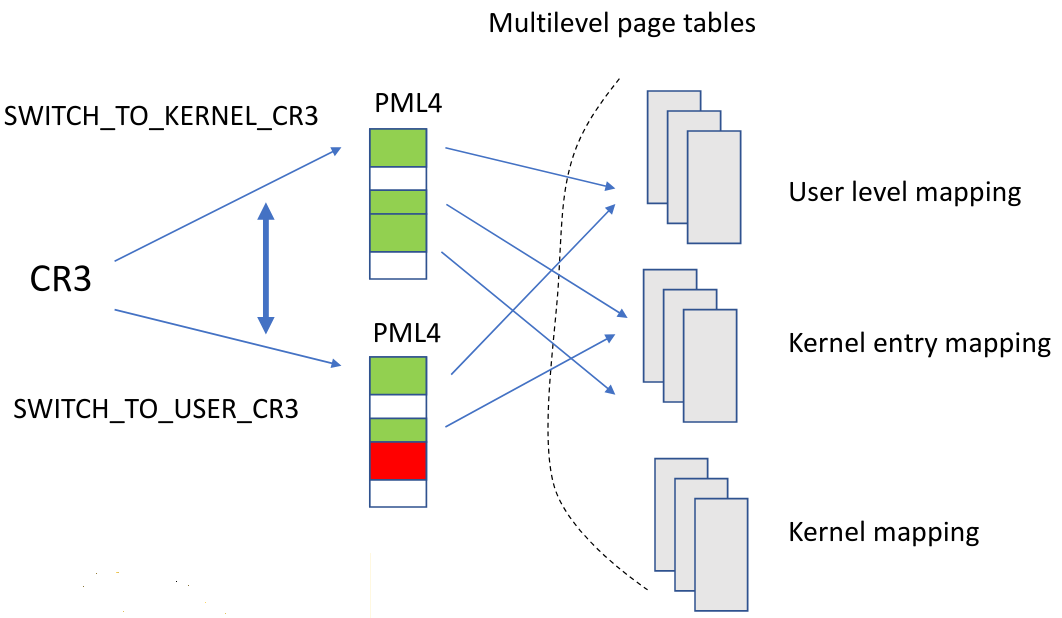
\includegraphics[scale=0.3]{immagini/KAISER}\\\\
due pt differenti, una per quando si lavora in maniera user ed una quando si lavora in kernel mode. Quando si chiama una sys call si passa ad una zona di address space in cui sono informazioni relative solo al codice kernel level, quindi non sensibile. In modo kernel, la zona di codice cambia la PT con una replicata in cui la zona è visibile, ma siamo già in modo kernel.\\ Il costo che viene pagato in termini del cambiamento della page table è che il TLB viene flushato. Nel TLB abbiamo una entry per una intera pagina, pagherò dei cache miss ma uno per pagina e non uno per ogni accesso come accade per la cache.\\ Inoltre, questa soluzione para da una serie di altri attacchi; la patch si può disattivare usando \textsf{pti=off} a livello del kernel usando GRUB. Su Linux è anche possibile mettere le patch on/off per la singola applicazione, se magari mi accorgo di un comportamento anomalo e non per tutte quelle running
\section{Branches}
Le istruzioni di salto sono un altro aspetto importante nell'esecuzione del program flow: se c'è un salto, è possibile che le istruzioni che devono entrare nel program flow provengano da diversi punti dell'address space. Quando si lavoro eseguendo in pipeline, non è possibile fillare solo quando si sa che il salto è deciso o non deciso, perché ci sarebbero stalli fino a che l'istruzione non va in commit point. I salti possibili sono riassunti di seguito 
\begin{itemize}
\item salti condizionali: non è noto se il salto avrà luogo o no quanto questa istruzione entra in pipeline. Il numero possibile di outcome però è 2: o si salta o no
\item salti non condizionali: salto sempre preso, a tempo di decode si sa già che si salta e quindi siamo in grado di acquisire le istruzioni per fillare la pipe 
\item call: anche qui il salto è sempre preso
\item return: anche questo salto è sempre preso, ma non sappiamo dove andare. Potremmo avere molte destinazioni, in quanto questo è funzione della stack area e sappiamo che il valore può essere aggiornato
\item salti indiretti: implementati in modo che l'istruzione è un salto, ma il target non è un offset nell'address space, bensì è indicato da un puntatore, quindi ad esempio il contenuto di un registro. La soluzione è molto usata quando dobbiamo realizzare dei function pointers
\end{itemize}
Quindi, eccetto i casi "più semplici" in cui si decide quando saltare a decode time, gli scenari sono più complessi perché bisognerebbe decidere dove saltare a commit time.\\ Esiste quindi nei processori il concetto di branch prediction: il processore ha osservato determinate istruzioni nella pipeline, e nel momento in cui queste vengono ri-osservate sa già cosa, in quanto ad esempio sa se nel caso precedente il salto è avvenuto o no.\\ Le architetture nei processori consentono di fare cose più complesse: quando lavoriamo in un processore pipeline super-scalare abbiamo un \textbf{dynamic predictor} che usa una Branch History Table o Branc-Prediction Buffer.\\ 
L'implementazione è basata su una cache indicizzata dai bit meno significativi dell'istruzione di salto e da un bit di stato, per cui ogni tabella ha una entry in cui viene indicato se saltare o no, e la tabella è indicizzata dal program counter. \\ Se passa una determinata istruzione viene registrato nella tabella se si è saltato o no (all'interno del bit di stato), in modo che se questa ripassa, si verifica col PC se c'è matching e se è così, in base al bit di stato, si decide quali istruzione caricare in pipeline.\\ Ovviamente, il salto può non avvenire, quindi poi bisogna flushare la pipeline se a commit time l'istruzione non salta. Siamo ancora in un contesto in cui le istruzioni lasciano tracce e sono problematici dal punto di vista della sicurezza.\\ Questa è una implementazione basica, inoltre nella tabella si mantengono solo alcuni dei bit che caratterizzano l'indirizzo contenuto nel PC: questo può far si che abbiamo un errore se prediciamo qualcosa che non si manifesterà, quindi il bit è 1 quando doveva essere 0 o viceversa, ma è anche possibile che nell'address space ci sia un'altra istruzione che ha la parte registrata nella tabella identica rispetto ad un altra istruzione che è quella effettivamente registrata e quindi abbiamo un altro tipo di errore. In generale, per errore intendiamo che vengono caricate in pipeline determinate cose e quindi si hanno dei side effects inattesi.
\subsection{Multiple bits predictors}
Il predittore ad un bit fallisce nello scenario in cui il branch viene preso frequentemente e non preso preso poco frequentemente. In questo tipo di scenario, tali predittori portano a 2 errori di seguito nella predizione, e quindi a due quashes della pipeline.\\ 
Una variante a due bit per un branch predictor ci dice che se una istruzione ha un certo indirizzo i, non registriamo un solo bit nella tabella bensì 2 bit, con cui possiamo discriminare 4 stadi possibili: 2 possono essere associati all'idea di saltare e gli altri 2 a quella di non saltare. In questo caso, per far si che venga invertita la previsione di salto, occorre avere 2 errori consecutivi\\ Possiamo quindi avere diversi outcome, ma se la macchina a stati è a 4 stati possiamo tenere traccia di più eventi possibili: ad esempio, se l'istruzione è passata ed è saltata ripassando si risalta. Se il salto non avviene, possiamo andare in un altro stato in cui viene detto che precedentemente è stato sbagliato il salto, ma si continua comunque a saltare.\\ Questo avviene ad esempio nei nested loop: c'è una volta in cui non si salta, ma le altre volte si salta sempre. Se ci fosse una macchina salta/non salta, l'ultima volta non salto e non posso ricordarmi che non ho saltato prima. Avrei quindi una serie di squash della pipeline. Un esempio di codice Assembly che realizza un loop annidato è mostrato in seguito:
\begin{lstlisting}
1	mov $0, %ecx
2 . outerLoop:
3	cmp $10, %ecx
4	je .done
5	mov $0, %ebx
6	
7 .innerLoop:
8	  ; actual code	
9	  inc %ebx
10	  cmp $10, %ebx
11	  jne .innerLoop
12
13	  inc %ecx
14	  jmp .outerLoop
15 .done:
\end{lstlisting}
Viene poi riportato l'automa a stati finiti che corrisponde al predittore a due bit:\\\\
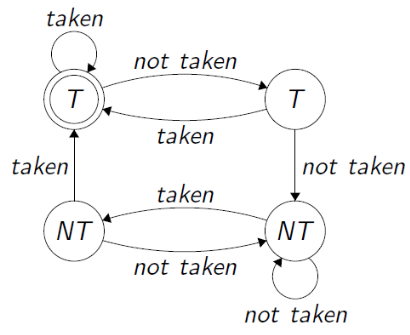
\includegraphics[scale=0.6]{immagini/2bit_pred}\\\\
Non è l'unico modo per essere efficaci nel momento in cui abbiamo dei loop nel codice: il saltare o non saltare può essere condizionato da cosa è accaduto prima. La macchina a stati sopra è riferita ad una singola istruzione, ma le cose dipendono dal passata di più istruzioni
\subsection{Altre soluzioni per branch predictors}
Se sbagliamo, su una architettura super-scalare e pipeline buttiamo decine di istruzioni magari pronte al commit, quindi è necessario andare oltre al predittore per le singole istruzioni, i due predittori che estendono il singolo sono
\begin{itemize}
\item predittori correlati a due livelli;
\item tournament predictors
\end{itemize}
Un esempio generale per considerare istruzioni di salto multiple può essere il seguente:
\begin{lstlisting}
if (aa == VAL)
	aa = 0;
if (bb == VAL)
	bb = 0;
if (aa != bb){
	// do the work
}
\end{lstlisting}
\subsubsection{Predittore correlato(m,n) a due livelli}
L'idea è che c'è una importante correlazione nel flusso di esecuzione, quindi guardando all'esempio precedente, si cerca di predire cosa accadrà nel 3° branch in base alla storia relativa a cosa è accaduto nei primi due.\\ Su architetture Intel, manteniamo per ogni flusso di esecuzione un registro di esecuzione che ci dice dati gli ultimi m salti se è avvenuto o meno il salto. \\ Il branch corrente viene predetto con un predittore ad n bit, quindi in totale ci sono $2^m$ predittori ad n bit.\\
Nella pipeline c'è quindi una maschera che registra se è avvenuto o no il salto, la maschera può essere fatta comunque da istruzioni che possono essere committed oppure speculari, quindi una zona più recente sarà committed ed una non committed. Se la storia è fatta da due bit, possiamo discriminare 4 valori differenti, collegandoli alla history sono flussi di esecuzione completamente differenti, quindi per ciascuna di queste possibilità associamo uno specifico predittore a ciascuna combinazione dei 2 bit. I predittori indicano per l'istruzione, dato cosa è accaduto nel passato per i salti, cosa fare, ovvero se saltare o meno. In generale quindi, i predittori sono tipicamente marcati con la notazione di (m,n) dove m sono gli elementi (i branch passati) mantenuti nella history ed n i bit mantenuti da ogni predittore.\\ Il predittore per la predizione corrente viene scelto sulla base dei risultati degli ultimi m branches, come è codificato nella $2^m$ bitmask.\\ Una figura riassuntiva è mostrata in seguito:\\
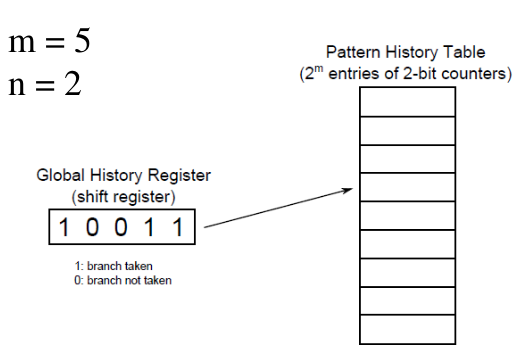
\includegraphics[scale=0.4]{immagini/corr_pred}
\subsubsection{Tournament predictor}
Il predittore di un branch tiene conto del fatto che per una istruzione di salto, a seconda di come è scritto il programma, ha senso eseguire il salto in funzione di quali sono le istruzioni passate in pipeline prima di questa. Non è detto che il predittore correlato sia sempre il migliore, perché per la singola istruzione la storia globale può essere una penalità in base alla struttura del codice.\\ Questo predittore mantiene per ogni istruzione le informazioni di un (m,n) ed anche 2 bit per avere 4 stati:
\begin{enumerate}
\item quando si predice per una istruzione di interesse, conviene guardare tutte le cose;
\item quando passa una istruzione, non guardare la history bensì solo un predittore locale;
\item guardare solo alla storia globale;
\item (non saltare)?
\end{enumerate}
Quindi, vengono messe in competizione la visione locale e quella globale. Se il flusso di esecuzione non ha molti errori, avremo una stabilizzazione che mostra "chi vince nella sfida"
\subsection{Salti indiretti}
Il salto indiretto è strano: se l'istruzione deve saltare, questo è funzione del risultato delle istruzioni precedenti, ovvero di cosa queste hanno scritto nei registri, che verranno usati per saltare.\\ Quindi, il valore di tali registri può variare sempre nel tempo, il che rende la predizione più complessa ed i side effects generati sono di più.\\ L'idea è di mantenere nella stessa architettura una cache, in cui vengono mantenute informazioni a cui associamo oltre all'indirizzo del branch anche il pre-fetched target, anche dei bit per indicare quanti errori ci sono stati.\\ Nel momenti in cui c'è cache miss non si può prelevare il salto, altrimenti viene presa l'istruzione successiva, una delle istruzioni più interessanti di questo tipo in x86 è \textsf{jump [register]}, interessante per implementare function pointers, che viene mostrata nella figura sottostante:\\
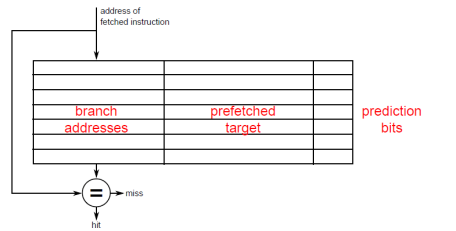
\includegraphics[scale=0.5]{immagini/jmp_reg}\\\\
Quando abbiamo un errore in predizione perdiamo performance, ed inoltre ci sono problemi di sicurezza da considerare
\subsection{Attacchi spectre}
Attacchi che ancora sono in vigore, si sta studiando come introdurre delle patch a livello hardware per poter bypassare spectre con però dei costi prestazionali importanti, ad esempio disconnettere la branch prediction dinamica. Il problema è che i dati vanno avanti, ad esempio in meltdown i dati vanno in cache e cambiano lo stato micro-architetturale.\\ In spectre accade la seguente cosa: il processore ha il branch predictor, se lo caratterizziamo come componente di più ampio livello abbiamo una fase di learning e da quello il predittore decide cosa fare la prossima volta. Ma cosa fare può essere sbagliato: insegno al predittore cosa fare in maniera volutamente errata, per poi passare un flusso dove le cose imparate non sono più valide e che quindi vengono gestite male.
\subsubsection{Spectre v1 (spectre prime}
Abbiamo un if che testa un condizione su un certo valore X, che può essere un indice usato all'interno di un array. Poi, si può scendere in un codice per cui si accede ad un array A e si usa B[X] shiftato a destra di 12, ovvero per indicizzare ogni volta 4096 byte e quindi una pagina.\\ Accediamo quindi ad A per un byte, identifichiamo il byte con B[X] ed idealmente abbiamo 256 possibilità che possono essere 256 pagine come visto in meltdown.\\ X è un indice di un'altra zona di dati, B può essere un'altra zona di memoria: sto caricando un'altra zona di informazioni spiazzandomi con X, carico il codice e usandolo per indicizzarmi in A. Quindi la posizione è in funzione di dove è B, ma anche di quanto è X: se mi sposto in una zona kernel space, funziona ancora se il branch predictor sbaglia la predizione perché è stato "allenato" così. Non abbiamo nemmeno seg fault perché è il branch predictor a fare il salto che è errato e quindi le istruzioni non vanno nemmeno in commit. Quindi, sullo stesso flusso di esecuzione possiamo fare inspection sull'array di probing A per vedere il valore che aveva B[X]. Lo spectre v1 è orientato alla problematica del branch prediction di salti condizionali.\\ Possono capitare anche cose più complesse: per come stiamo usando ora spectre, leggiamo informazioni livello kernel senza andare in seg fault, quindi il processore deve essere tale per cui l'istruzione passa comunque come offending, ma se è patchata lato hardware viene bypassata.\\ Il problema è che non basta aver risolto meltdown: quando viene eseguito del sotfware in una architettura convenzionale accade che viene chiamata una syscall ad un certo punto. Quando il  kernel parte, avrà delle informazioni nei registri di processore per sapere cosa fare, ma potrebbero essere stati scritti dei valori nel registro che viene usato in un check per cui si fanno determinate cose in base al valore, quindi il salto del kernel è impattato da tale valore e di conseguenza anche cosa la branch prediction fa.\\ Quindi, stabilito cosa deve avvenire quando si salta, si cambia il valore e questo permette di far eseguire al kernel speculativamente qualsiasi blocco di codice. Supponiamo di chiamare una syscall: a livello kernel c'è una tabella fatta di function pointers, ho passato tramite il registro quale valore della tabella considerare. Possiamo passare al branch un valore che è oltre la tabella, viene eseguito il salto perché il branch perdictor non sa che non deve andare oltre. Quindi, il codice del kernel si muove in funzione di cosa passa l'utente, ma così l'utente può passare parametri che alterano la branch prediction per poi attaccare. Quindi, la patch per meltdown è già stata bypassata, è stato necessario riscrivere il codice del kernel con patch per quanto riguarda il valore osservato livello kernel rispetto a quello passato dallo user, ad esempio marcando alcuni bit e tagliando il valore passato in modo che si rimane in zone incluse nella tabella.
\subsubsection{Spectre v2}
Con spectre si portano avanti anche attacchi di questo tipo: abbiamo il processore e gli hyperthread, ma il branch predictor sta nel "motore", non viene esposto a livello ISA. Il core è visibile da flussi differenti, nell'istante di tempo t abbiamo un programma P sul core, mentre a t' possiamo avere P' in esecuzione: la branch prediction sta nel core, quindi P può eseguire una serie di istruzioni può dare input al branch predictor per comportarsi in un certo modo, quando c'è context swtich e cambia il programma, possiamo sfruttare il branch predictor allenato, la predizione sarà sbagliata ma abbiamo side effect sul secondo contesto che è osservabile dal primo. Un riassunto dello scenario è mostrato in seguito:\\
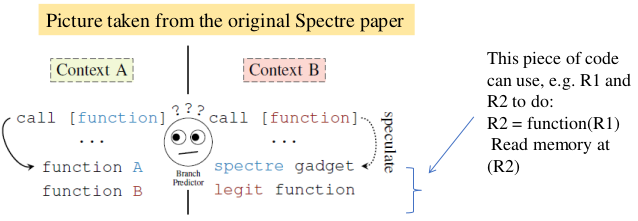
\includegraphics[scale=0.5]{immagini/spectrev2_branch_pred} \\\\
lo scenario è che l'attaccante ha costruito il flusso di esecuzione per avere l'istruzione di salto indiretto nello stesso indirizzo dell'address space rispetto a quello della vittima, quindi quando si salta, si va in istruzioni macchine dette \textbf{gadget}, ovvero delle istruzioni che possono essere utili all'attaccante in quanto vengono creati dei side effect, ad esempio se cambio qualcosa in cache e questa è accessibile all'attaccante, il cambio è visibile.\\ Il concetto di sfruttare un gadget sulla predizione è importante per la return oriented programming, dove vengono sfruttati i gadget. Ovviamente, il miss training va fatto sullo stesso CPU core della vittima, mentre il probing della cache può avvenire anche su core diversi.
\subsubsection{Come bypassare spectre v2}
Per salti diretti, l'unica cosa che il software può fare è ridurre il valore che viene passato nei registri per accedere alla memoria. Per quelli indiretti la patch è la \textbf{retpoline}, ovvero un trampolino basato su istruzione di ritorno. Supponiamo di dover lavorare con del software tale per cui quando questo esegue serve fare un salto indiretto: il salto non viene eseguito, bensì il sotfware effettivo per arrivare alla destinazione prevede l'uso di un trampolino, quindi varie istruzioni in più. I trampolini sono basati sull'istruzione di \textsf{ret}, la soluzione vale per qualunque architettura. I passi eseguiti sono i seguenti:
\begin{enumerate}
\item viene salvato nello stack il traget addrress dove saltare
\item si esegue una chiamata di un pezzo di codice che rimuove il valore di ritorno del PC dallo stack, che era la chiamata originale
\item la porzione di codice salta all'indirizzo con l'istruzione di \textsf{ret}
\item perciò, la chiamata originale non ha un ritorno attuale e quindi il codice delle istruzioni successive alla chiamata sono un loop infinito
\item i predittori per i salti indiretti per questo motivo non saranno sfruttabili per andare ad eseguire del codice in maniera speculativa
\end{enumerate}
\begin{lstlisting}
	push target_address
1:	call retpoline_target
	// put here whatever you like
	// typically a serializing instruction with no side effects
	jump lb
retpoline_target:
	lea 8(%rsp), &rsp // we do not simply add 8 to RSP
					  // since FLAGS should not be modified
	ret  // this will hit target address
\end{lstlisting}
la \textsf{lea} carica l'indirizzo effettivo, viene fatto con questa istruzione perché questa non ha side effect sul processore, eliminando gli 8 byte che rappresentano il punto di ritorno della chiamata.\\ 
\subsubsection{esempio: codice per spectre}
Nel codice, viene fatto un controllo per capire quanti cicli di CPU sono necessari per un cache hit e quanti per un cache miss. Il tempo non è comunque perfetto, perché il sistema è pur sempre time sharing e quindi fra due timer possono essere successe varie cose.\\ La secret area è una pagina che metto nell'address space per potermi poi spiazzare con x ed andare nel kernel space.
\subsection{Loop unrolling}
Il problema della branch prediction è comunque legato al fatto che vogliamo cercare di saltare prima ed inoltre ridurre il numero di branches presenti in un flusso di esecuzione: se c'è un if then else non è possibile ridurlo, ma ad esempio possiamo avere un salto condizionale dalla prima istruzione all'ultima (ciclo) e vogliamo ridurre gli impatti prestazionali da un punto di vista dei salti. Il problema è che andiamo a controllare l'esecuzione del codice e quindi paghiamo altre istruzioni macchina come overhead, per ridurre il numero di tali istruzioni viene usata tipicamente la tecnica del loop unrolling: se il ciclo deve girare per n volte, il compilatore o chi scrive il codice allarga il corpo ciclo, inserendo molteplici statements che altrimenti sarebbero eseguiti in diverse iterazioni del loop.\\
L'unrolling si può sviluppare sia a mano, ma non è buono perché stiamo scrivendo più linee di codice e quindi aumentando la probabilità di bug in quanto si lavorano in zone di memoria differenti. È anche possibile fare l'unloop in automatico, usando un tool di compilazione come gcc dicendo, prima di compilare una zona di codice, una opzione di compilazione \textsf{\#pragma GCC optimze ("unroll loops")}. Se facciamo l'unroll del loop, il ciclo viene eseguito un numero minore di volte nell'eseguibile, ma deve eseguire più attività e quindi bisogna usare più registri e magari usare più linee di cache, quindi ci può essere un più ampio impatto sull'architettura.\\ Ci sono una serie di effetti collaterali di cui tenere conto, osservabili analizzando il codice eseguibile, guardando magari nell'ELF dove è stato implementato l'unroll per verificare il fattore di unroll.
\section{Aspetti esterni al processore in una architettura IT}
Cerchiamo di capire quali sono gli impatti degli altri componenti nelle architetture IT. Siamo in uno scenario in cui abbiamo il problema del power wall: non possiamo aumentare la frequenza dei clock più di un tot perché avremo un power consumption tale per cui non avremmo più bilancio di calore nel chip.\\ Di fatti, il consumo di potenza cresce secondo la legge $VxVxF$ e per cui non si riesce ad andare sopra i 130W, limite superiore per uci is garantisce dissipazione di potenza.\\ La legge di Moore dice che si possono aggiungere transistor nella CPU per poter aumentare la potenza, ma ora non è più possibile: quindi, invece di avere un solo processore, ce ne sono di più. Nell'architettura non ci sono poi solo i processori, ma anche le memorie.
\subsection{Multi processori}
Su un multi-processore simmetrico ci sono tanti oggetti simili che possono processare un flusso di programma, vedono tutti la stessa memoria, ma hanno anche delle cache private affinché i dati siano più vicini al processore.\\ Il problema è che se il dato è lo stesso e viene avvicinato ai diversi processori, questo viene replicato e c'è un problema globale nell'interazione fra processore e memoria.\\\\
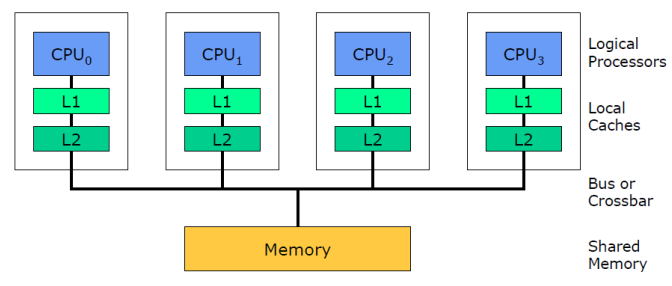
\includegraphics[scale=0.5]{immagini/multi_proc}\\\\
Ora c'è il chip multi-processor, in cui ogni processore ha più di una CPU, le CPU hanno delle L1 private e magari delle L2 condivise: questo è un modo con cui il vendor permette di accorpare le risorse del chipset rispetto al caso precedente.\\\\
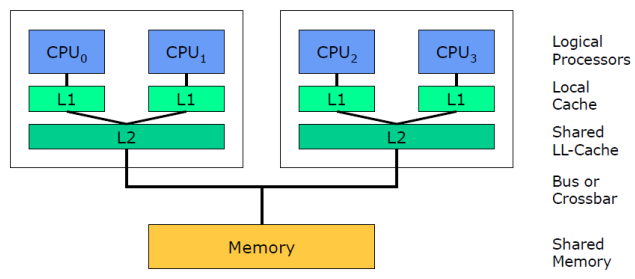
\includegraphics[scale=0.5]{immagini/cmp.png} \\\\
Infine abbiamo anche il symmetric multi-threading, perché se il core va molto veloce possiamo portare più di un flusso di esecuzione con gli hyperthread. Resta il problema dell'architettura di memoria per quanto riguarda la cache privata.\\\\ 
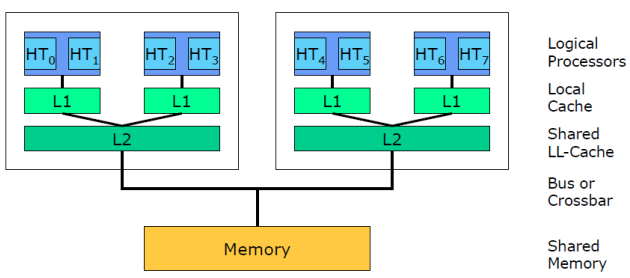
\includegraphics[scale=0.5]{immagini/smt}\\\\
Questo tipo di chipset ha fatto si che venisse scalata in verticale anche la capacità della memoria: le attività che portano sulla memoria fanno traffico su un unica strada e questo ha portato alla creazione dell'architettura NUMA
\subsection{Architettura NUMA (Non Uniform Memory Access)}
La memoria è composta da vari slot e ciascuno ha una via principale per portare dati verso il processore. Inoltre, ogni processore può leggere dati dagli slot non vicini a lui, ma deve farlo tramite una via esterna alla sua. Supponiamo che il core 1 debba usare solo pagine della zona di memoria a lui vicine, allora le due zone di memoria toccate sono separate e riusciamo a raddoppiare la capacità computazionale della memoria.\\ Il problema è quando vanno toccate zone di memoria non direttamente: servono strutture di interconnessione ed inoltre bisogna bloccare la strada per quel nodo NUMA da parte del core ricevente.\\ Lavorando in una architettura NUMA, i dati numerici ci dicono orientativamente che si aspetta dai 50 ai 200 cicli di clock per ricevere dei dati dalla memoria se si accede ad una zona vicina, altrimenti si va sui 200\%300 cicli. Si parla di sistemi scarichi, quindi aumentano parecchio se le vie sono busy per via del carico sul sistema.\\
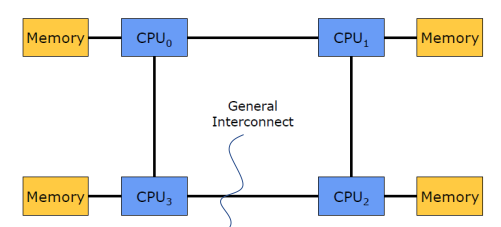
\includegraphics[scale=0.5]{immagini/numa}
\section{Coerenza delle cache}
Le attività basiche che caratterizzano l'hardware riguardano quello che avviene nella zona di cache: questa non è visibile nell'ISA, non è possibile toccare direttamente la cache col software per cui non si ha in maniera esplicita la possibilità di governarla.\\ C'è il problema della coerenza delle cache: la cache è un sistema di replicazione, quindi astraendo la struttura interna abbiamo un insieme di slot messi a disposizione per mantenere dati. Il dato D può essere registrato in due slot diversi, quindi quale replica si usa se qualcuno chiede di leggere un dato? Ancora peggio se avviene una scrittura sul dato: si aggiorna una sola replica o entrambe? Altra cosa interessante è che quando si parla di coerenza della cache si parla solo dell'oggetto hardware cache, ma nella CPU avvengono diverse cose (ooo, speculation etc...), ad esempio le scritture vengono fatte sullo store buffer e vengono poi portate in memoria e questo problema riguarda la \textbf{memory consistency}.
\subsection{Definizione della coerenza}
La coerenza nell'architettura di cache è definita in base a 3 proprietà:
\begin{itemize}
\item stiamo leggendo da una locazione di memoria X, precedentemente scritta dallo stesso processore ritorna l'ultimo valore scritto se nessun altro processore ha fatto nulla su quella locazione. \textbf{Causalità del program flow.}
\item {Avoidance of staleness}: se leggo da X e la lettura segue una scrittura su X da un altro processore, il valore letto è quello che è stato scritto dal processore se le due operazioni sono separate da un certo intervallo temporale
\item Tutte le scritture su X da tutti i processori sono serializzate, quindi non si possono vedere le write dai diversi processori in ordine diverso. Quindi viene gestito un ordine in modo che i dati vengano acceduti col valore corretto dai diversi processori quando c'è un update; non ci sono buffer dove vengono mantenute le cose e non vengono rese effettive (come accade ad esempio nello store buffer)
\end{itemize}
\subsubsection{Cache write through e write back con le consistenze}
Cosa accade, rispetto alla memoria, quando viene scritto un dato. Vediamo se le cose fatte da un single core basta anche per un multi-core. I due processori hanno due cache e c'è poi la memoria, vediamo la tecnica del \textbf{write through}, per cui il valore scritto in locale viene anche propagato sulla memoria.\\
Se ci muoviamo con più componenti associate a processori differenti, possiamo avere che: $CPU_0$ legge X e carica 0 in cache, fa lo stesso $CPU_1$. Poi, $CPU_0$ scrive 1 su X e propaga la scrittura, ma quando $CPU_1$ legge X dalla cache legge 0 e la distanza fra le due operazioni può essere arbitraria, stiamo violando il requisito 1.\\ 
Se usassimo write back: $CPU_0$ legge X e carica 0, $CPU_1$ legge X e carica 0. Poi $CPU_1$ scrive 1 e la scrittura non viene propagata, poi $CPU_1$ scrive 2 su X. Quindi abbiamo due valori aggiornati, uno in memoria, se $CPU_1$ fa il write back della linea in cui c'è X e poi successivamente lo fa anche $CPU_0$, il valore 2 viene sovrascritto e quindi siamo in grado di invertire l'effetto dell'update sui dati indipendentemente dalla distanza temporale fra gli update.
\subsection{Protocolli di consistenza}
Le cache, oltre a mantenere i dati eseguono anche dei protocolli, quindi la logica di controllo nella cache è più articolata della letture/scrittura cache. Sono implementati a livello firmware, ed hanno 
\begin{itemize}
\item una serie di transazioni che sono supportabili fra diversi componenti hardware
\item gli stati in cui si può trovare un blocco di cache
\item un insieme di eventi gestiti dal controller
\item un insieme di transizioni fra stati
\end{itemize}
L'architettura può essere organizzata in maniera differente in base a diversi fattori
\begin{itemize}
\item topologia dell'interconnessione
\item primitive di comunicazione
\item gerarchia di memoria, se inclusiva o no
\item politiche di cache
\end{itemize}
i protocolli possono poi migliorare diverse performance
\begin{itemize}
\item latenza della singola transazione
\item throughput 
\item overhead dello spazio dovuto ai bit di gestione, che toglie spazio alla cache effettiva
\end{itemize}
Le famiglie classiche di protocolli sono due, che risolvono il problema di quando aggiornare le repliche nelle altre cache 
\begin{itemize}
\item invalidate protocols: quando un core scrive un blocco, tutte le altre copie diventano invalide, questo implica che si evitano le situazioni descritte prima. Solo il writer ha la possibilità di accedere alla copia aggiornata. Si incrementa la latenza ma si riduce la banda utilizzata, però chi vuole il dato non lo ha vicino nei componenti dell'architettura di caching
\item update protocols: quando avviene una scrittura, vengono aggiornate tutte le altre copie. Si pagano però costi importanti per l'aggiornamento dei dati: ogni copia del blocco è sempre aggiornata alla copia coerente. Abbiamo il trade-off fra banda e latenza: ognuno prende la copia dal vicino ma si paga sulla banda
\end{itemize}
I primi sono quelli usati in architetture moderne, per cui ci focalizziamo su quelli per capire come avviene l'invalidazione
\subsubsection{Snooping cache}
Come lavorano effettivamente i vari componenti dell'architettura hardware per implementare l'invalidate protocol: tutti i componenti sono connessi fra loro tramite un mezzo broadcast, anche detto rete, quindi tutte le cache possono parlare con tutte. È un modo semplice per poter prendere il mezzo, comunicare a tutti ad esempio un cambio di stato per far si che tutti lo cambino. C'è la serializzazione di tutte le transazioni: quando la CPU va sull'interfaccia verso la cache, l'interazione deve usare il broadcast medium, ma se non è necessario che ci sia la transazione distribuita non si parla. Se quando si manda l'interazione verso l'architettura di cache e questo genera un evento tale per cui qualcun altro deve parlare c'è la serializzazione, quindi nella time line i cambi di stato avvengono quando quello precedente è completato. I componenti di caching sono connessi a dei controller che è in grado di capire i messaggi di broadcast per poter effettuare i cambi di stato. Finché il controller non ha preso il mezzo di comunicazione il cambiamento di stato non può avvenire. Di seguito, viene mostrato uno schema architetturale:\\\\
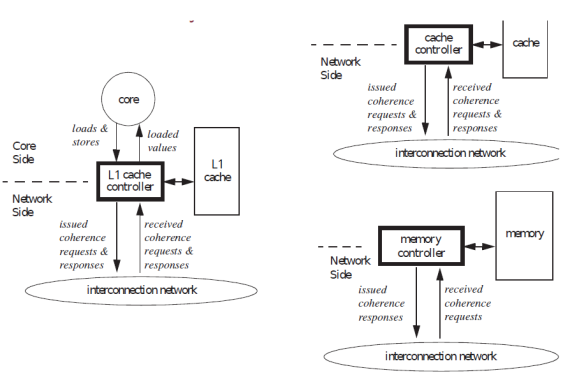
\includegraphics[scale=0.5]{immagini/cache_conn}\\\\
Le azioni trattano le singole linee di cache, per cui quando qualcuno parla lo fa per quella linea di cache.
\subsubsection{MSI protocol}
Tipicamente, si tiene traccia dei seguenti stati per un blocco in cache:
\begin{itemize}
\item modified, ovvero scritto e quindi che rende invalide le altre copie
\item invalid
\item shared: la versione più è condivisa fra vari componenti, qualcuno ha avuto una copia dal writer o da un altro reader
\end{itemize}
Una transazione di scrittura invalida tutte le altre copie del blocco di cache, mentre una transazione di lettura
\begin{itemize}
\item prende l'ultima copia aggiornata dalla memoria in caso di cache write thorugh
\item prende l'ultima copia aggiornata dalla memoria o da un altro componente  di caching nel caso write back (come ad esempio in Intel)
\end{itemize}
\subsubsection{Protocollo MESI}
Gli stati di una linea di cache possono essere 4
\begin{itemize}
\item Invalid
\item Modified
\item Shared
\item Exclusive: il componente di cache indica che fa una gestione esclusiva di quella linea di cache. Ovvero quel componente può fare ciò che vuole senza dover dire a nessuno che ha scritto la linea. Quindi, questo può avvenire senza interazioni con nessuno: se un program flow tocca un dato per aggiornarlo di continuo, non è necessario comunicare ad altri componenti che questo è accaduto, e prende di conseguenza la linea di cache ad uso esclusivo
\end{itemize}
Quindi, non è vero che qualcuno legga qualcosa di vecchio, perché questo è vero solo se qualcuno passa ad exclusive e rende invalide le altre copie.\\ L'automa a stati finiti che riassume il passaggio fra i vari stati è mostrato di seguito:\\\\
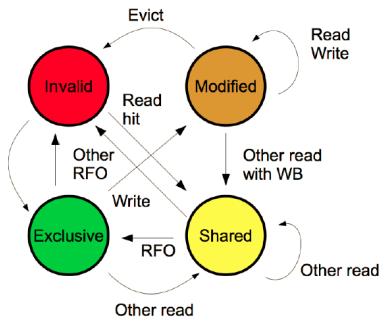
\includegraphics[scale=0.5]{immagini/MESI}\\
una RFO non è altro che una richiesta di ottenere l'ownership della linea di cache.\\
\textbf{esempio: transazioni in risposta a letture locali}\\
se lo stato è M, E o S non succede nulla. Se invece siamo in I, va generata una richiesta sul bus, se ci sono altre cache che hanno una copia del dato mandano un segnale di sharing e se questo avviene, il componente transita nello stato S; altrimenti, va nello stato E.
\textbf{esempio: transazioni in risposta a scritture locali}\\
\begin{itemize}
\item se lo stato è M non ci sono transazioni
\item se lo stato è E non ci sono transazioni sul bus e si fa in M
\item se lo stato è S, la linea è in locale ma posso avere le altre copie e quindi tramite l'uso del bus genero una richiesta di read per prendere l'uso esclusivo
\item se lo stato è I si genera una richiesta di uso esclusivo e si va in M
\end{itemize}
ALTRI ESEMPI SULLE SLIDES
\subsubsection{MOESI}
Variante del MESI in cui c'è uno stato in più che è Owned, ovvero una cache line può essere Owned e la differenza rispetto ad Exclusive è che se aggiorno della linea di cache, gli altri la hanno invalida. In O è possibile che se aggiorno la linea do la copia a chi la chiede ma lo avviso che essendo l'owner potrei aggiornare la linea in futuro e che chi al riceve non può più aggiornarla; questo evita la transizione in diversi stati come avveniva prima.
\subsubsection{Implementazioni in x86}
Tipicamente, in Intel
\begin{itemize}
\item MESI
\item Cache inclusive
\item Write back
\item Cache L1 con linee a 64 byte
\end{itemize}
AMD
\begin{itemize}
\item MOESI
\item Cache esclusiva ad L3
\item Write back
\item Cache L1 con linee a 64 byte
\end{itemize}
\subsubsection{Alternativa allo snooping}
Lo snooping va bene quando la scala dell'architettura non è grande, ma se la scala cresce e si parla tutti con tutti ci sono problemi di delay.\\ Quindi, lo snooping non scala bene, per cui si risolve usando soluzioni \textbf{directory-based}:
\begin{itemize}
\item non c'è più il broadcast, i componenti comunicano indirettamente fra loro
\item al centro della comunicazione c'è la directory, che mantiene i meta-dati
\end{itemize}
Quindi, per parlare con i componenti, non è detto che debba parlare con tutti ma lo faccio solo con la directory. Inoltre, la directory serializza tutte le attività solo internamente.
\paragraph{Funzionamento della directory:}per ogni unità portata dalla RAM alla cache, vengono mantenuti dei meta-dati, dove indichiamo che sta mantenendo la copia del dato e se il dato è dirty.\\\\
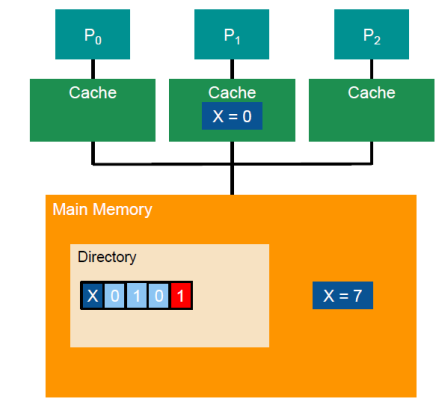
\includegraphics[scale=0.5]{immagini/dir_based}\\\\
Possiamo quindi dire che c'è una versione aggiornata presso un componente della cache, che è in corrispondenza di chi ha il dato aggiornato (l'1 azzurrino) e quindi poi si aggiorna, se qualcuno richiede il dato, chi lo mantiene.\\ \textbf{esempio:}\\ Abbiamo un read miss per $P_0$, quindi andando dalla directory scopre chi ha la copia del dato, consegnarlo e marcare il bit pari ad 1. In questo modo, sappiamo che quando qualcuno scrive dobbiamo invalidare solo alcuni dei processori ovvero quelli che hanno il dato shared.
\subsection{Relazione fra software e performance della cache}
La scrittura del software produce un program flow che poi finisce in cache, a seconda di ciò che viene scritto. Supponiamo di avere un program flow in cui si cerca di accedere in memoria per prelevare un dato e quel dato è in una certa linea di cache. Supponiamo poi di avere un altra istruzione che vuole leggere un altra area di memoria, quindi in corrispondenza di un'altra linea di cache: abbiamo la località dei dati user space\\ Il problema è grave se giriamo con più thread o hyperthread o più processi in concorrenza che accedono in memoria: le istruzioni chiamate toccano le stesse strutture dati, le interazioni chiamate cambiano lo stato MESI delle linee di cache, quello che bisogna evitare quando si scrive codice di kernel è che i dati usati più spesso devono essere sulla stessa linea di cache in modo da diminuire gli accessi in cache.\\ Le informazioni scarsamente correlate fra loro non devono invece cadere sulla stessa linea di cache, perché se due thread vogliono scrivere su due diversi byte e questi sono nella stessa linea di cache interagiscono con il protocollo MESI chiamando un maggiore numero di transazioni, sharando la linea di cache.\\ In modo che il software sia scritto bene, occorre sapere se l'area di memoria logica è allineata con la linea di cache: viene dato un pointer dalla malloc e vogliamo che i 64 byte logici che otteniamo siano allineato coi 64 byte della linea di cache così da avere un buffer cache aligned. Questo dipende dal tipo di allocatore che si usa:
\begin{itemize}
\item \textsf{posix\_memalign }
\item \textsf{aligned\_alloc }
\item \textsf{valloc }
\end{itemize}
C'è quindi il problema del false cache sharing: se abbiamo due strutture che sono una di x byte ed una di y byte e questi sono usati da due core diversi, e la somma x+y $<$ 2*chache\_line, i dati cadono sulla stessa linea di cache e quindi c'è un problema prestazionale.\\ 
\subsection{Insepction cache line access}
Abbiamo visto meltdown e spectre, tutto è nato usando il risultato dell'inspecting cache line access, ovvero è possibile con questa tecnica che si basa sull'osservare le latenze di accesso alle aree di memoria condivisa capire se un dato è in cache oppure no. Per fare questo, si possono utilizzare i passi seguenti:
\begin{itemize}
\item il contenuto della cache relazionato ad un certo dato condiviso fa flushato
\item si ri-associa il contenuto in read mode
\item osserviamo la latenza di accesso: se è bassa, vuol dire che qualcun altro ha portato il dato in cache, altrimenti  ce lo sto portando io
\end{itemize}
L'implementazione su x86 è basata su due blocchi fondamentali:
\begin{itemize}
\item un timer ad alta risoluzione, per effettuare le misure temporali
\item usare istruzioni non privilegiate per fare cache line flush
\end{itemize}
\subsubsection{High resolution timer per x86}
Esiste un high resolution timer, che permette di misurare con una grana fine, ovvero quella dei cicli di clock, quando tempo è passato.\\ Il cronometro è RDTSC, si accede ad un registro special purprose che mantiene il numero di cicli di clock passati fino a quel momento (può andare in overload), il valore è mantenuto in un registro della famiglia msr, ovvero dei registri non-general purpose. I valori vengono caricati in edx ed eax, 32 bit in uno e 32 bit nell'altro, che siano i più o meno significativi della maschera di 64 bit del contatore, quindi possiamo prendere una delle due parti in base al nostro interesse.\\ Nella pagina del manuale di x86 viene detto che l'istruzione può non essere permessa quando si lavora user mode, generando un protection error, scrivendo un bit in CR4 per cui resettando o settando il bit è possibile che l'istruzione sia o non sia usata user mode. L'istruzione è molto usata da software che fa profiling dell'applicazione, quindi è necessario lasciare la possibilità che sia usata user mode, per cui ci si espone al fatto che possa essere usata da software malevoli.
\subsubsection{Cache line flush}
L'istruzione per fare cache line flush è CLFLUSH: viene passato un pointer ad un byte, che è in una zona di 64 byte che in memoria fisica costituiscono una unica linea che viene caricata, quindi la linea viene flushata. Se viene chiamata l'istruzione, siamo sicuri che l'operazione sia corretta rispetto a tutte le operazioni che sono state fatte su quel byte e su quella linea? Siamo in una finestra temporale in cui, prima del flush, avevamo cominciato una write che poteva aver toccato un byte di quella stessa linea, ed in pipeline le due istruzioni potrebbero essere invertite, per cui se non stiamo attenti rischiamo di flushare un contenuto vecchio, che poi verrà riscritto. Quindi, per poter riportare in memoria con la flush l'istruzione scritta e quindi quella aggiornata, bisogna usare una ulteriore istruzione: MFENCE. Con questa istruzione, stiamo cambiando il modo con cui il processore sta accedendo alla cache.
\subsection{ASM inline}
Come si scrive Assembly in modalità C: è possibile mischiare notazione C e Assembly, quando verrà eseguita la versione della funzione alcune istruzioni Assembly saranno già state scelte dal programmatore.\\ Tipicamente un blocco ASM prevede alcune informazioni obbligatorie ed altre opzionali. Vediamo il blocco:
\begin{lstlisting}
__asm__ [volatile] [goto] (AssemberTemplate
		[ : OutputOperands ]
		[ : InputOperands ]
		[ : Clobbers ]
		[ : GotoLabels ]);
\end{lstlisting}
Output ed Input permettono di rapportare l'esecuzione delle istruzioni specificate nell'Assembler template, ovvero qualcosa che avvenga prima o dopo. I clobbers è l'insieme dei registri che eventualmente devono essere salvati se c'è un side effect, quindi che siano push e pop per rimettere a posto lo stato. Volatile va a dire al compilatore di non andare ad ottimizzare le istruzioni macchina passate, cosa che altrimenti può avvenire in automatico.\\ Dettagli su Input/Output
\begin{itemize}
\item il simbolo uguale può essere usato in fase di output, quindi ad esempio che si sta relazionando una variabile ad un registro in output
\item nella zona di input non è necessario usare il simbolo di =, andando a specificare movimenti di variabili differenti
\item per specificare se usare registri o memoria al compilatore, ci sono delle notazioni apposite:
\begin{itemize}
\item r: registro generico
\item m: area di memoria generica
\item 0-9: indici per riferire cose usate prima nella notazione
\item i/l sono gli immediate a 32 o 64 bit
\item q: registri byte addressable
\item A: eax o edx
\item altro...
\end{itemize}
\end{itemize}
Dato tutto questo, ecco come viene riscritta la flush + reload:
\begin{lstlisting}
usigned long probe(char *adrs){
	volatile unsigned long cycles;
	asm(
		"mfence \n"
		"lfence \n"
		"rdtsc \n"
		"lfence \n"
		"movl %%eax %%esi	\n"
		"movl (%1) %%eax	\n"
		"lfence \n"
		"rdtsc \n"
		"subl %%esi, %%eax \n"
		"clflush 0(%1)		\n"
		: "=a" (cycles)
		: "c" (adrs)
		: "%esi" , "%edx"   );
	
	return cycles;
}
\end{lstlisting}
la mov dell'1 dice che va preso il valore di ecx ed usarlo come pointer per caricare il valore in eax, quindi è la load di cui vogliamo misurare il tempo. Va preso il cronometro prima e dopo con rdtsc. Sposto anche dei dati per fare la sub, ovvero sottraendo i cicli di clock iniziali e finali.\\ Di seguito, vengono mostrate delle tipiche timelines che si possono avere durante l'esecuzione di un flush+reaload.\\\\
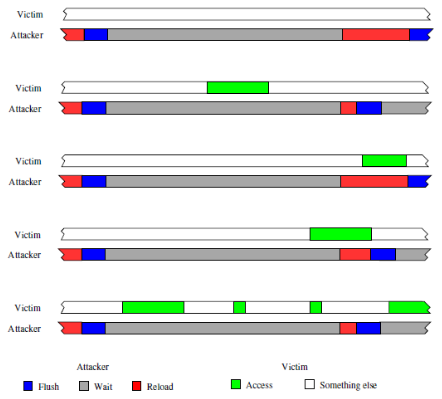
\includegraphics[scale=0.5]{immagini/flrel}
\subsection{Inspection cache senza RDTSC}
Quando usiamo RDTSC, misuriamo dei valori assoluti: vedendo insieme i due valori ottenuti per accesso ai dati con e senza flushing, e vediamo che uno scenario è circa 3 volte più lento di un altro. Potremmo quindi anche non misurarli correttamente ed avere una misura indicativa di cosa accade. Quindi, se viene prevenuto l'uso di RDTSC, i tempi possono essere misurati secondo un altro schema:
\begin{itemize}
\item usiamo più thread: uno dei due incrementa solo una variabile, l'altro invece fa flush e reload ed il tempo viene misurato usando il valore passato dal primo thread, per vedere se viene incrementato di più o di meno. Come facciamo per far si che il thread non riesca a determinare la differenza fra i due casi: se il thread non è in CPU quando il secondo thread cerca di prendere il valore della misura, allora la differenza sarà sempre 0.
\end{itemize}
\subsection{Nota: inclusività della cache}
La cache inclusiva è tale per cui ad un livello più baso il componente di caching $L_x$ ha sempre una copia aggiornata del contenuto cachato dal livello superiore $L_y$, quindi $L_y$ è sempre incluso in $L_x$.\\ Per sistemi che usano cache non inclusive potrebbero causare il fallimento di attacchi di tipo flush + reload, che possono continuare ad essere fruttuosi se, ad esempio, lanciati su processi che girano sullo stesso CPU core.
\section{Memory concistency}
Abbiamo visto la cache coherency, che ci ha fatto vedere cosa accade in una architettura in quanto abbiamo processore $|$ zona memorizzazione con i vari componenti (L1, L2, RAM) quando qualcuno chiede o aggiorna dati.\\ Osservare cosa succede guardando solo l'interfaccia fra processore e memoria da una visione limitata di cosa accade realmente quando un program flow deve lavorare con la memoria. \\ Quindi può accadere che su un program flow operazioni di accesso in lettura e scrittura non siano riversate sull'interfaccia quando pronte. Noi ci aspettiamo che una lettura riporti l'ultimo valore scritto, ma sull'interfaccia o da parte del program flow? Perché se ci sono più flussi paralleli questo cambia: se ad esempio una istruzione che scrive con una mov, non è detto che il risultato sia subito esposto sull'ISA, ma può essere scritto nello store buffer. Quindi se un processore P scrive e P' legge, può darsi che la lettura di P' venga postata sull'interfaccia per leggere, ma il valore di P non è stato ancora scritto.\\ Abbiamo due aspetti:
\begin{itemize}
\item program ored, ovvero l'ordine di accessi in memoria per come accadono nel program flow
\item visibility order, ovvero l'ordine con cui i processori accedono per andare sull'architettura moderna e che viene osservato da uno o diversi processori. Ogni lettura restituisce il valore della scrittura più recente
\end{itemize}
\subsection{Sequencial consistency}
Una modalità di raccordare le cose è la sequencial consistency, in cui essenzialmente per tutto ciò che viene fatto su un program flow non è possibile che una cosa fatta non sia visibile dagli altri flussi su un oggetto condiviso, ovvero sulla memoria.\\ Supponiamo di avere un flusso di programma che scrive su A ed uno che scrive su B, ed un altro scrive su C, non è vero che se guardo il visibility order per gli altri c'è prima B e poi A o C: l'ordine è A-C-B.\\ Un altro esempio:
\begin{itemize}
\item la $CPU_1$ esegue le operazioni
\begin{itemize}
\item [A] = l;($a_1$)
\item [B] = l;($b_1$)
\end{itemize}
\item mente la $CPU_2$ fa
\begin{itemize}
\item u = [B];($a_2$)
\item v = [A];($b_2$)
\end{itemize}
\end{itemize} 
Se l'ordine con cui vengono viste le operazioni, e quindi i risultati, è $a_1, b_1, a_2, b_2$ allora c'è sequencial consistency. Se invece l'ordine è, ad esempio, $b_1, a_2, b_2, a_1$ non c'è sequencial consistency.\\
Le architetture che abbiamo non sono sequencially consistents: se scriviamo un valore e mandiamo in commit l'istruzione e poi scriviamo in una seconda istruzione, potremmo usare una linea di cache differente per la seconda istruzione e non necessariamente aspettare in MOESI/MESI, quindi se dobbiamo servire dei cache miss e non c'è la possibilità di lavorare sulla linea di cache come si vorrebbe, bisogna fermare altre attività.
\subsection{Total Store Order}
Nelle architetture moderne, si lavora col Total Store Order: quando mandiamo delle scritture, queste possono scrivere in uno \textbf{StoreBuffer} intermedio e solo poi tali scritture sono riportate in memoria. Come vengono riportate è deciso dal vendor, può essere l'ordine con cui sono arrivate le cose oppure no.\\ Quindi, se lo StoreBuffer è Out-Of-Order è ancora più complicato la relazione fra program order e visibility order. Le macchine moderne tipicamente hanno questo StoreBuffer, quindi a valle della registrazione nel buffer alcune scritture vengono ritardate. Lo store buffer va bene se scrivo e leggo la stessa cosa, ma è diverso se occorre leggere da altre aree di memoria. \\ Processori x86 tipicamente implementano lo \textbf{store bypass}: una istruzione scrive nello StoreBuffer, un'altra che legge lo fa direttamente dalla memoria, ma così nel visibility order non è rispettata la consistenza sequenziale.\\ Lo StoreBuffer è utile per evitare di dover per forza ogni volta di interagire con una memoria per le scritture, se ad esempio il valore serve al program flow viene ripreso direttamente dallo StoreBuffer. Aiuta quindi nelle performance, ma c'è il problema della consistenza da gestire.\\ Un esempio di algoritmo che non funziona senza sequencial consistency (Algoritmo di Dekker):\\\\
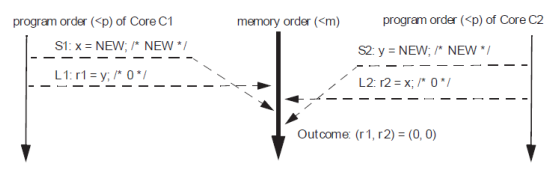
\includegraphics[scale=0.5]{immagini/dekker}
\\ Ognuno segnala una variabile e legge quella dell'altro
\subsection{Sincronizzazione della memoria in x86}
Il problema va affrontato processore per processore, perché caratterizza l'architettura del processore stesso. Occorre gestire lo StoreBuffer, in x86 lo si può fare con delle apposite istruzioni macchina
\begin{itemize}
\item SFENCE: store fence, permette di fare qualcosa per quanto riguarda la visibilità delle cose che sono nello StoreBuffer. Quindi, si dice che tutte le store precedenti alla sfence devono essere rese visibili prima che vengano mostrare quelle dopo l'sfence. Questo permette quindi di gestire idealmente degli StoreBuffer non FIFO, rendendoli quindi FIFO ma in molte implementazioni Intel lo usano già;
\item LFENCE: mentre sfence lavora sulle store, lstore lavora sulle load. La specifica di manuale non parla del visibility order, lfence permette invece di riorganizzare l'ordine di esecuzione delle load: lfence non esegue finché le load precedenti ad lfence non sono complete, ma anche nell'ordine speculativo. Quindi possiamo sincronizzare le istruzioni di load nella pipeline. Qui non si parla di visibilità globale, è importante per quando misuriamo delle latenze
\item MFENCE: Nessuna fra lfence ed sfence permettono di risolvere lo \textbf{store bypass}, ovvero la possibilità che delle operazioni di load superino delle scritture e quindi vengano lette delle informazioni stale. \\ Con mfence si sincronizzano tutte le attività verso la memoria, ovvero dallo store buffer verso la memoria, ma anche le letture verso al memoria. Evitiamo quindi il problema dello store bypass
\end{itemize}
Questo è fondamentale quando si scrive codice del kernel, perché siamo concorrenti su tutti i core. \\ Ci sono una serie di istruzioni che permettono di sincronizzare load e store: se ad esempio consideriamo una MFENCE, questa permette di scaricare un load buffer in memoria, ma ci sono delle istruzioni che fanno cose più complesse: lettura di una zona di memoria ed aggiornamento del valore. Quindi ad esempio possiamo leggere valori, confrontarli con delle bitmask e se il confronto va a buon fine, aggiornare il valore. Le istruzioni sopra permettono di fare questo, inoltre possiamo prendere lo StoreBuffer e scaricarlo in memoria in modo che tutti i dati precedenti siano andati in memoria. \\ Abbiamo, fra le tante, \textbf{CMPXCHNG}: l'operazione prende un valore, lo porta nel processore, lo compara e poi lo aggiorna. Ci si aspetta che tutto ciò si basi sul fatto che il valore che viene preso per compararlo sia il dato aggiornato, quindi la linea di cache va bloccata a tutti gli altri processori, per essere letta ed aggiornata atomicamente. Questo è implementato in x86, ma va anche a flushare ciò che è nello store buffer ed è generato da istruzioni precedenti, per cui si sincronizza la memoria. \textbf{CMPXCHNG} permette di implementare i lock, in modo che se viene trovato lo 0 nella locazione, ci mette un 1 e prende il lock; controllando il bit di stato della CPU è possibile capire se la compare\&swap è andata a buon fine, in modo da sapere se è stata presa la linea di cache.\\ Possiamo ridurre il costo di questa istruzione macchina, in modo che non mantenga la linea bloccata in stato exclusive, tramite il prefisso \textsf{\textit{lock}}.\\  Più in generale, le istruzioni che fanno questa attività si chiamano istruzioni della classe \textbf{Read-Modify-Write}: tre operazioni insieme, ce ne sono varie che possono fare diverse cose. La osa interessante è che quando viene eseguita una operazione di questo tipo, si interagisce con MESI, perché bisogna andare sull'interfaccia CPU-memoria e prendere la linea di cache in maniera esclusiva, verranno quindi spesi diversi cicli di clock per fare questa attività e quindi bisogna stare attenti all'uso delle operazioni perché impattano sulle performance. I costi spesi ci sono: bisogna flushare lo StoreBuffer in memoria, quindi la linea di cache da scrivere deve transitare nello stato giusto, quindi di deve interagire col MESI. La cosa interessante è che però si lavora solo in cache, quindi non si blocca l'accesso in memoria.
\paragraph{gcc built-in}ci sono una serie di intrincisc gcc che permette di usare una API da usare nel codice in modo che il programmatore sia più vicino a ciò che accade nell'architettura hardware, viene indotto qualcosa.
\subsubsection{Esempi di implementazione}
Vediamo l'implementazione di una \textbf{Active Barrier}, che è una barriera fra thread per ottenere sincronizzazione. 
\begin{lstlisting}
long control_counter = THREADS;
long era_counter = THREADS;

void barrier(void){
	int ret;
	
	while(era_counter != THREADS && control_counter == THREADS);
	ret = __sync_bool_compare_and_swap(&control_counter,THREADS,0);
	if(ret) era_counter = 0;
	
	__sync_fetch_and_add(&control_counter,1)
	while(control_counter != THREADS);
	__sync_fetch_and_add(&era_counter,1)
}
\end{lstlisting}
Se occorre controllare un certo numero di threads, si scrivono due variabili control\_counter ed era\_counter, perché è possibile che il thread esca dallo schema prima degli altri, quindi se rientra si porta all'era successiva ma qualcuno può ancora usare l'era precedente. Il thread che vuole scrivere sulla memoria cerca di portare control\_counter a 0, dopo esserci riuscito ( e solo uno ci riuscirà alla volta) cambia anche l'era\_counter per impedire anche allo stesso thread di rientrare finché anche gli altri non sono rientrati. In control\_counter viene aggiunta una unità, in modo che tutti gli altri thread aspettino che tutti passino.\\\\
Un altro esempio è la \textbf{trylock basata su ASM}:\\
\begin{lstlisting}
int try_lock(void * uadr){
	unsigned long r = 0;
	asm volatile(
		"xor %%rax,%%rax\n"
		"mov $1,%%rbx\n"
		\textbf{"lock cmpxchg %%rbx,(%1)\n"}
		"sete (%0) \n"
		: : "r"(&r), "r" (uadr)
		: "%rax","%rbx"	
	);
	return (r) ? 1 : 0;
}
\end{lstlisting}
la C\&S è basata sul valore di rax, usiamo poi l'indirizzo per accedere alla memoria (\%1 = uadr) e rax è il registro di comparazione. Alla fine, viene ritornato 0 o 1 a seconda del valore ottenuto da r, quindi è possibile poi riprovare la trylock se non viene preso il lock.
\subsection{Locks contro coordinazione scalabile} 
In una architettura moderna è necessario considerare che una memoria può essere acceduta da più thread. Fin ora abbiamo risolto con dei lock, ma l'approccio non è vincente se il numero di thread concorrenti diventa molto alto ed inoltre i thread potrebbero essere interessati a zone differenti della struttura dati, se usiamo i lock uno dei thread viene bloccato e questo è un problema di scalabilità importante. Sono nati da molto tempo degli approcci in cui il coordinamento si sfruttano istruzioni RMW non per implementare il lock bensì gli step da eseguire nella struttura dati, quindi l'algoritmo di gestione della struttura dati. Lavoriamo su due zone separate, la cosa è coerente perché i thread sanno di essere gli unici a lavorare sulla memoria, le soluzione che abbiamo sono
\begin{itemize}
\item Read Copy Update (RCU) usate in maniera massiva nel kernel Linux
\item Coordinamento non bloccante, dove abbiamo algoritmi di tipo lock e wait free. Non vengono usati i lock, quindi si lavora su una struttura dati condivisa secondo delle regole differenti
\end{itemize}
I meccanismi garantiscono che quando vengono rilasciati i lock, le modifiche contenute nello StoreBuffer sono state flushate in memoria.
\subsubsection{Linearizzabilità}
Criterio di correttezza di un algoritmo, se l'algoritmo è linearizzabile è corretto. Stiamo ragionando sulla concorrenza di threading, possiamo avere che tutto ciò che facciamo in un algoritmo linearizzabile è simile a ciò che faremmo in un algoritmo serializzabile. Il concetto è però più articolato: supponiamo di considerare una struttura dati condivisa, ed avere in una timeline un thread che comincia a lavorare ad un certo istante t e finisce ad un altro istante t'. La durata della timeline è $\delta$, ma in realtà il punto effettivo in cui il thread va a lavorare sulla struttura dati condivisa è univocamente identificabile in un unico punto dell'intervallo. Possiamo identificare un istante temporale in cui gli altri threads sanno che quello specifico thread sta lavorando sulla data struct, questo è molto vicino alla RMW: se tocco una locazione di memoria che rappresenta la struttura dati su cui i thread stanno lavorando, se uno la tocca non può accadere null'altro, perché in MESI è in stato esclusive. Per questo, una RMW può essere usata in un algoritmo per implementare l'istante in cui il thread sta modificando la struttura dati.\\ Vediamo uno schema più complesso: abbiamo 3 operazioni possibili su una struttura dati condivisa, eseguono due thread concorrenti: abbiamo che fra due operazioni concorrenti una delle due si renda visibile prima o dopo, ma l'importante è che sia atomica. Possiamo quindi materializzare le operazioni le operazioni in diversi istanti di tempo, rispettando i constraint sul singolo flusso di programma, abbiamo quindi delle storie ammissibili\\\\
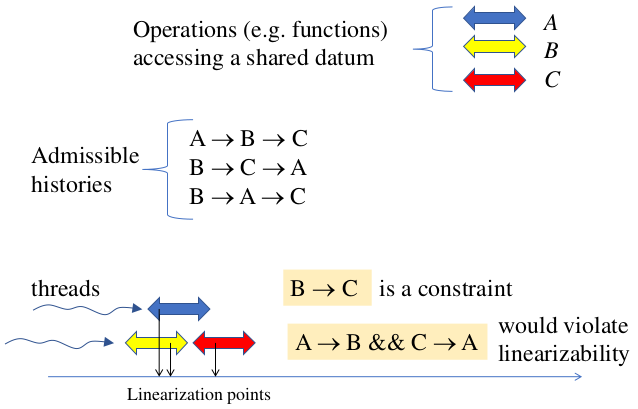
\includegraphics[scale=0.6]{immagini/wct.png}\\\\
Quindi, nella linearizzabilità, se due thread concorrono su una stessa struttura dati sarà visibile a gli altri threads mediante RMW quando qualcuno sta facendo operazioni sulla struttura dati, ma non sappiamo in che punto della timeline questo accadrà.\\ RMW permette che non accada niente altro nella specifica zona di memoria, in quanto come detto la linea di cache viene presa in uso esclusivo in MESI. \\ Possiamo avere due soluzioni differenti in algoritmi concorrenti:
\begin{itemize}
\item lock freedom: eseguiamo una operazione su qualche struttura condivisa, ma la RMW può fallire, anche la C\&S può fallire, perché magari l'operazione è andata in conflitto con quella di un altro thread che ha fatto qualche altra istruzione. Siamo in una situazione in cui non si è in grado di concludere l'esecuzione e quindi di rendere visibile agli altri la modifica. Nel caso lock free si ripete l'operazione, perché mentre sto lavorando io, qualcun altro ha già fatto qualcosa. La cosa interessante è che almeno un thread termina in un tempo finito, indipendente dalle attività degli altri: il numero di cicli di clock usati non dipende da lock o da cose dovute agli altri. Tutte le istanze terminano, con successo o no, in un tempo finito;
\item wait-freedom: tutte le istanze delle chiamate a funzione finiscono in maniera successfull, quindi non è possibile andare in abort. Questo magari perché le istruzioni non vanno mai in conflitto, quindi viene fatto sempre lavoro utile e non verrà mai determinato un abort
\end{itemize}
Gli algoritmi sono utili perché, per il fatto che tutte o alcune delle istanze portino avanti attività corrette, nessuno si aspetta: in un sistema moderno, sui thread che eseguono attività per toccare strutture dati condivise ci sono diversi vantaggi:
\begin{itemize}
\item crash sul thread, se si prende un lock ed il thread crasha è tutto bloccato
\item su un architettura moderna si lavora con VM: la VM fa girare l'algoritmo in maniera dedicata, se il thread che ha preso il lock viene deschedulato dal vero SO della macchina, quindi la vCPU viene deschedulata, si tiene il lock bloccato per molto tempo usando istruzioni macchina ed energy nei processori
\end{itemize}
Senza lock tutto ciò non avviene: se giro l'algoritmo sulla VM ed un thread viene deschedulato non ci sono problemi, gli altri thread della VM vanno avanti.\\ Gli aspetti fondamentali della lock freedom sono quindi che
\begin{itemize}
\item si può fallire, questo porta alla possibilità di ricominciare. Mentre se la RMW non fallisce, ovvero nell'algoritmo difficilmente si va in conflitto sulla stessa linea di cache, si completa senza fallimenti
\end{itemize}
\textbf{esempio: linked list non bloccante}\\
Abbiamo una linked list condivisa, vediamo l'inserimento condiviso: scandiamo la lista e troviamo l'elemento dove inserire, nessun altro sa che sto facendo un inserimento. Abbiamo letto il pointer dell'elemento che serve, quindi possiamo leggere in C\&S per aggiornare l'elemento, a seconda del fatto che la C\&S fallisca o no, capiamo se qualcuno ha aggiornato o meno quell'indirizzo.\\\\
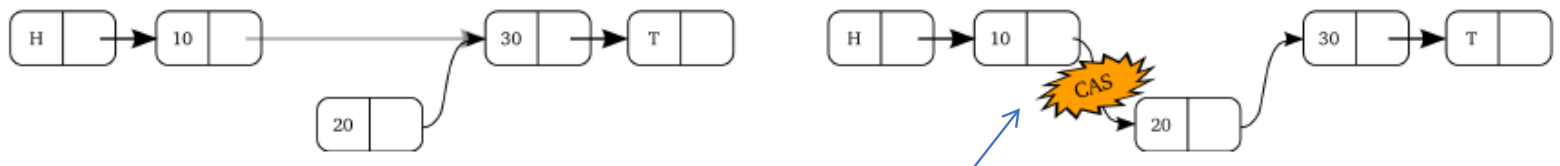
\includegraphics[scale=0.3]{immagini/cas_insert}
\\\\Leggermente più complesso è la remove di un nodo: non basta una C\&S, in quanto può accadere che un thread potrebbe inserire un elemento ed io voglia eliminare quello a cui il primo thread aggancia la sua insert. L'elemento va marcato con una C\&S come "da rimuovere", quindi ogni oggetto della lista avrà un pointer al successivo ed una bit mask che ne rappresentano lo stato\\\\
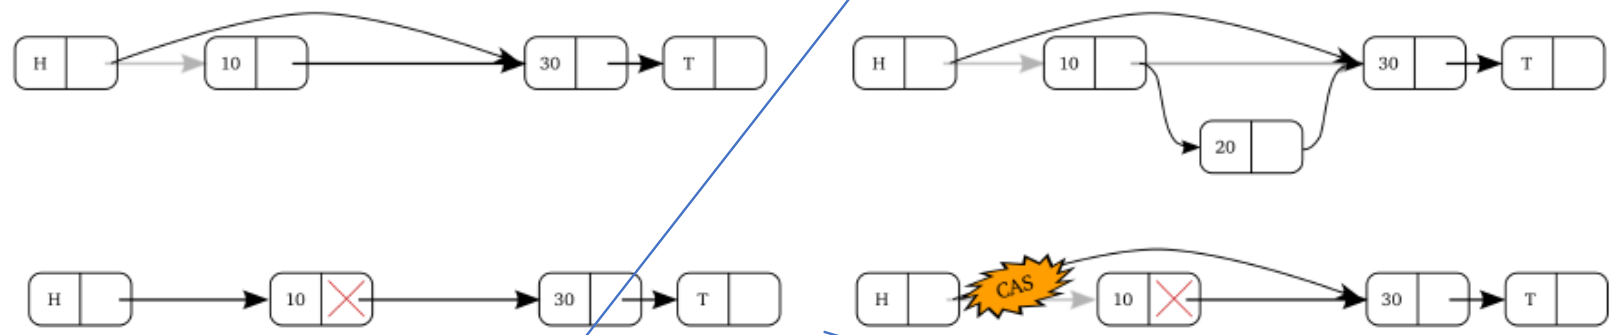
\includegraphics[scale=0.3]{immagini/cas_delete}\\\\
Supponiamo di avere dei thread concorrenti che fanno delle operazioni: un thread vuole rimuovere un elemento, lo marca e poi va in C\&S per eliminarlo (attaccare la head al successivo), sono due operazioni non atomiche. In un $\delta$ temporale un thread concorrente può attraversare la lista fino all'elemento che è marcato, che lo usa per lavorarci; nel mentre il thread che sta facendo l'eliminazione la completa e lo rilascia all'allocatore di memoria. Ma nel mentre qualcun altro può richiedere ed ottenere quella stessa area di memoria e scriverci delle informazioni. C'è quindi un problema di garbage collection dei nodi, occorre capire quando è effettivamente possibile rilasciare il nodo all'allocatore di memoria. Questo viene risolto da RCU, tecnica che non è bloccante solo per chi legge la struttura dati, mentre per chi aggiorna deve serializzare. Ma le strutture dati kernel sono molti lettori e pochi scrittori, quindi non ha senso bloccare la marea di lettori, si bloccano solo i pochi scrittori.\\ Un altro esempio è quello del \textbf{registro atomico}: abbiamo un'area di memoria m che è il registro, che è aggiornabile. Come aggiornarlo: o con locks, oppure con algoritmo apposito: implemento il registro come pointer, quando devo aggiornare il registro alloco una area appresso di m byte, in maniera atomica vado ad aggiornare  il pointer. Funziona solo se non c'è memory leakage, in letteratura è possibile implementarlo con al più n+2 slots, dove n sono reader ed uno è il writer. La soluzione è wait free: n+2 slot per leggere l'informazione, n possono essere concorrentemente letti, uno slot serve per tenere l'ultimo valore ed un altro per produrre un nuovo valore da pubblicare.\\ La soluzione si basa su avere all'interno dell'esecuzione dei thread una sola variabile di sincronizzazione, usabile in modo atomico tramite ISA (quindi RMW), abbiamo l'ultimo slot scritto e quanti reader hanno letto quello slot.\\ Per leggere, un thread preleva un indice ed in maniera atomica si marca come reader, lo scrittore può, da un altra parte, pubblicare un altro indice, 0 lettori e prelevare l'indice vecchio per vedere quanti lettori sono attestati su quello vecchio.\\ Ora negli slot è possibile capire quanti thread hanno finito di leggere e quanti stanno leggendo. Il reader dell'algoritmo fa una fetch\_\&add per prendere l'indice, ma la volta dopo confronta l'indice preso col valore presente nella variabile di sincronizzazione e se non è ancora cambiata si rilegge dallo stesso slot. Da un punto di vista delle performance, si ottengono dei risultati adeguate e che scalano molto bene. Di seguito, vengono mostrati gli pseudo-codici per l'implementazione del registro atomico:\\\\
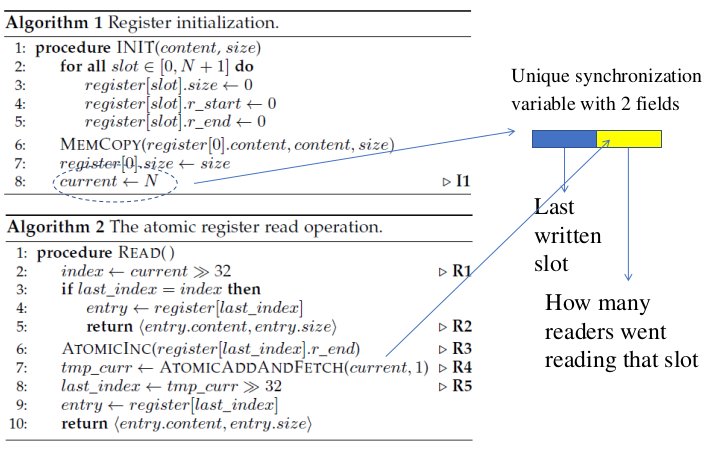
\includegraphics[scale=0.7]{immagini/atom_reg_1}\\
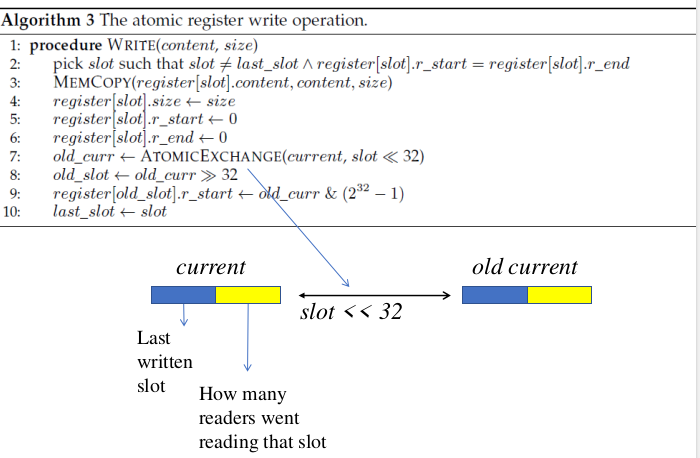
\includegraphics[scale=0.7]{immagini/atom_reg_2}\\
Gli approcci ci portano a capire che quando vogliamo un algoritmo concorrente e magari wait free, c'è una complessità maggiore del caso in cui stiamo lavorando con dei lock.
\section{Approccio di RCU}
È l'approccio alla base della costruzione di un sistema operativo moderno, ovvero che può girare su migliaia di CPU core dove i thread che sono in esecuzione condividono tutte le strutture dati.\\ La Read-Copy-Update permette di avere su una struttura dati condivisa un solo writer alla volta, quindi questi si sincronizzano fra di loro con dei lock, mentre i reader no. Questo favorisce delle strutture dati read-intensive che sono molte, una di queste è la hash table che mantiene quanti thread sono creati e quale è l'ID del thread.\\ La gestione dei collegamenti nella struttura dati è fatta nel seguente modo:
\begin{itemize}
\item gli outlinks della struttura dati che vengono rimosse logicamente, ad esempio come una remove di un nodo dalla lista collegata, non prevede al reale rimozione dei buffer ma vengono mantenuti attivi fino al \textbf{grace period}, ovvero periodo dopo il quale sono sicuro che chi sta attraversando la lista non lo fa pi attraverso il link che sto eliminando. Quindi ora l'aera di memoria può essere resa all'allocatore senza problemi
\end{itemize}
Il grace period su un SO reale viene implementato in maniera semplice, e questo si può fare anche a livello user e quindi RCU è uno schema che si può usare sia a livello kernel che a livello user per avere strutture dati scalabili in termini di accessi.\\ Abbiamo quindi il concetto di \textbf{standing readers}, che possono continuare ad usare aree di memoria rimosse, fino a che non avranno terminato l'esecuzione. Di seguito, viene mostrata la classica timeline di RCU
\begin{figure}[!h]
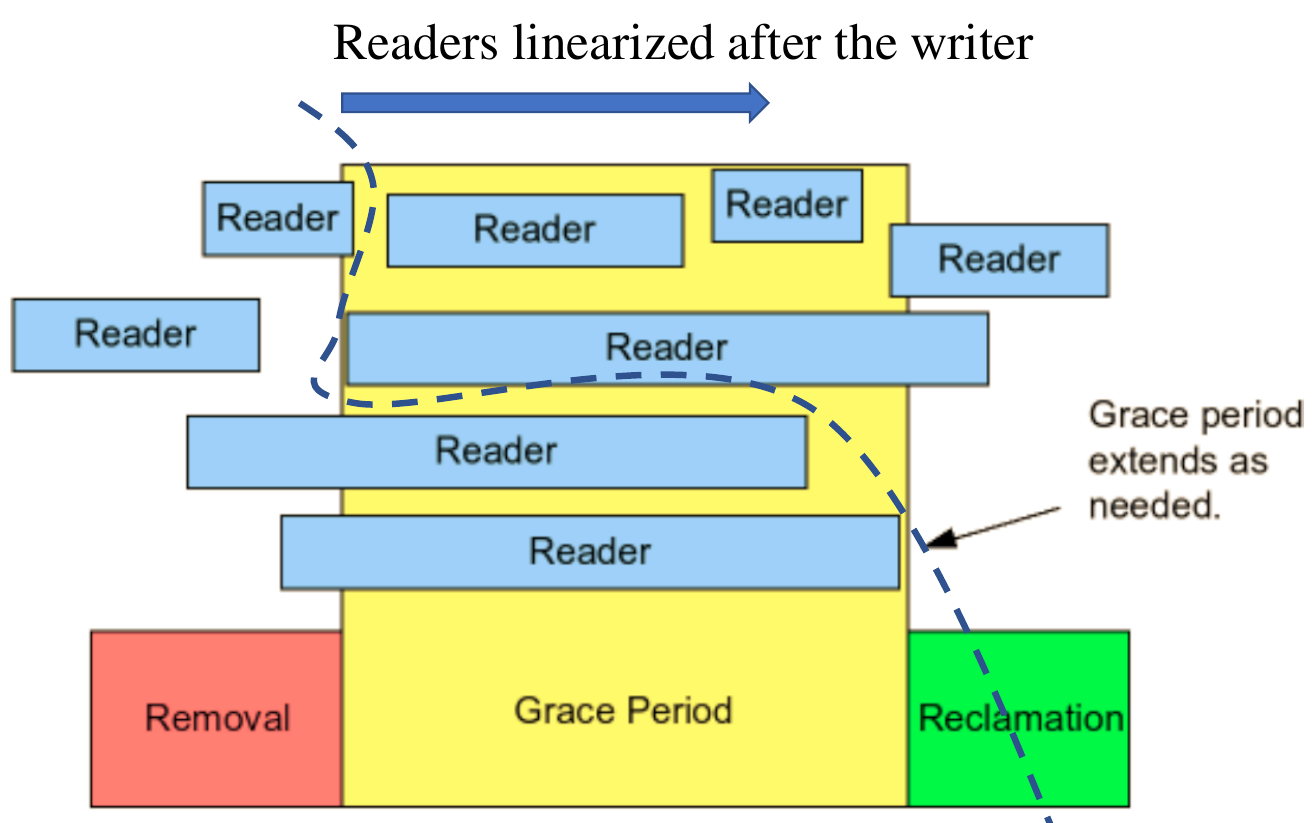
\includegraphics[scale=0.3]{immagini/rcu_timeline}
\end{figure}
i readers sono pienamente concorrenti al writer, quindi può accadere che la fine dell'esecuzione di alcuni dei readers va considerata dal writer prima della riconsegna dell'area di memoria, può anche capitare che un reader cominci a leggere dentro il grace period, quindi già con lo snapshot della struttura dati aggiornata e quindi il grace period può essere esteso se necessario.\\Vediamo come implementare lo schema, quindi come capire quando i reader iniziano e finiscono le operazioni rispetto a quando sta operando il writer: i concetti di base sono i seguenti\\
Il reader
\begin{itemize}
\item deve segnalare che c'è
\item deve leggere
\item deve segnalare che non c'è più, perché ha finito
\end{itemize}
Il writer
\begin{itemize}
\item prede il write lock
\item gestisce l'update della struttura dati, rimuovendo delle cose per generare un nuovo shape della struttura dati
\item attende i reader standing
\item i reader che si segnalano come presenti sulla struttura aggiornata vengono linearizzati dopo il writer
\item release del buffer
\end{itemize}
Vediamo ora come effettivamente vengono implementate le cose
\subsection{Kernel level RCU}
A livello kernel, è possibile per un execution flow disabilitare la preemption e riabilitarla: il CPU core non può essere ceduto ad un altro execution flow finché non è deciso, eseguire e poi tornare preemptable. Quindi, se nella fase non-preemptable si esegue una RCU, abbiamo un buon modo per poter leggere la struttura: disabilitando, si segnala di leggere, abilitando si dice di aver finito ed in questo modo nessun altro può avere il CPU core\\ il writer prende il lock, aggiorna la struttura dati ed alla fine deve chiedersi se c'è ancora qualche reader da linearizzare prima che il buffer venga de-allocato. Dopo aver finito quindi gira su tutte le CPU, ovvero chiamando servizi kernel per eseguire sulle diverse CPU e sarà possibile ottenere le CPU solo quando queste verranno rilasciate dai reader. Il problema è che questo avviene quando il numero di CPU core non è così elevato da permettere questo aggiornamento. La linea di codice per girare su tutte le CPU è la seguente: \textsf{for\_each\_online\_cpu(cpu) run\_on(cpu);}\\ Vediamo come fare senza abilitare/disabilitare le preemption
\subsection{Preemptable RCU}
Le RCU devono essere preemptable, quindi il thread può perdere la CPU, usiamo un concetto classico e relativo all'epoca: se appartengono all'epoca vecchia della struttura, occorre aspettare che l'epoca finisce; se invece sono tutti nella nuova epoca il writer non deve attendere.\\ Andiamo a ragionare sull'atomicità di cosa si può fare , in particolare è possibile aggiornare un contatore in maniera atomica, che sarà un \textbf{presence counter}, ovvero che indica la presenza nell'epoca. Quando il writer aggiorna la struttura dati, deve farla transitare nella nuova epoca e si ottiene con la ridirezione dei reader su un altro counter: un puntatore sa quanti reader stanno leggendo la struttura, si aggiorna la struttura e poi si aggiorna il puntatore al contatore successivo. C'è il rischio di dover aspettare un reader che sta già osservando la nuova shape, ma che ancora non rilascia il contatore vecchio, questa può essere la timeline della situazione:
\begin{figure}[!h]
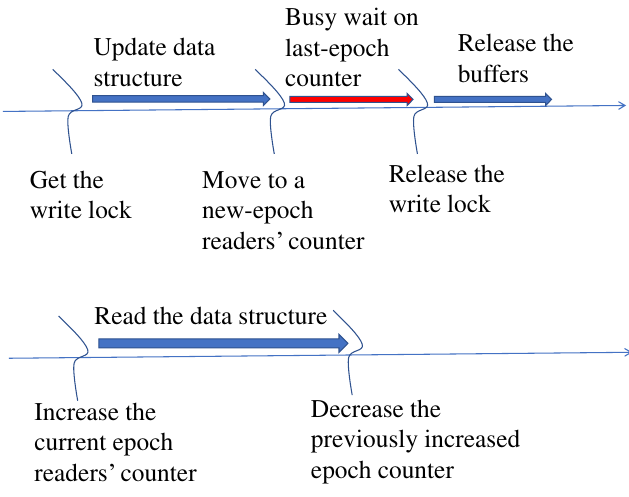
\includegraphics[scale=0.5]{immagini/preempt_rcu.png}
\end{figure}
Se uno dei thread crasha, può non essere in grado di decrementare il contatore, vuol dire che i buffer non possono essere lasciati all'allocatore ma non ci sono blocchi, la struttura può comunque essere rilasciata, è possibile comunque introdurre dei TO per sincronizzare il tutto.
\section{Aspetti ulteriori di parallelismo}
Abbiamo parlato più volte di parallelismo, abbiamo anche altri aspetti di parallelismo sul processore che è il concetto di \textbf{vettorizzazione}: possiamo eseguire delle istruzioni secondo la forma del processamento SIMD (Single Instruction Multiple Data); ci sono anche altri paradigmi come MIMD, che è a disposizione sui multi-processori o multi-core.\\ SIMD è basata sul concetto dei \textbf{registri vettoriali}, quindi registri che contengono diversi slot a 32/64 bit, quindi l'istruzione in maniera automatica sta già usando la vettorizzazione. SIDM è presente nei processori moderni, anche ad esempio nella GPU che è tipicamente SIMD, che specializza questo concetto. \\ Un altro aspetto interessante è la MISD (Multiple Instruction Single Data): due istruzioni sono su un flusso, che è un thread, due istruzioni scrivono su un registro in parallelo ed è possibile farlo in parallelo perché su architetture speculative si scrive su un renamed register.\\ Abbiamo infine SISD, che è il triviale (slides)
\subsection{Vettorizzazione su x86}
I processori sono fatti in modo che per le istruzioni SIMD, nell'architettura l'esecuzione si basa su l'uso di hardware "apposito", es. sommatori vettoriali per fare delle sommatorie che hanno più dati in input e forniscono più output. Lo schema astratto è il seguente:
\begin{figure}[!h]
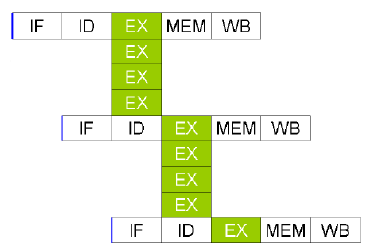
\includegraphics[scale=0.5]{immagini/exec_vettorizzata.png}
\end{figure}
Su x86 il supporto per l'esecuzione vettorizzata è \textbf{SSE} (\textbf{SSE-2} in 64 bit): abbiamo 8 registri vettoriali a 128 bit, dove possiamo mettere un vettore di informazioni. In SSE possiamo quindi inserire diverse combinazioni di valori
\begin{figure}[!h]
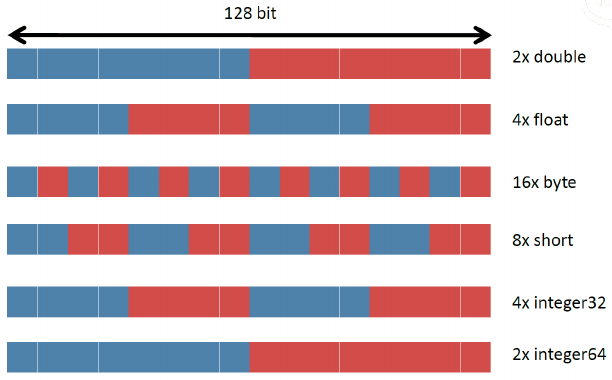
\includegraphics[scale=0.5]{immagini/sse_data.png}
\end{figure}
con l'estensione AVX i registri sono raddoppiati in numero e possono essere usati per due lane differenti
\begin{figure}[!h]
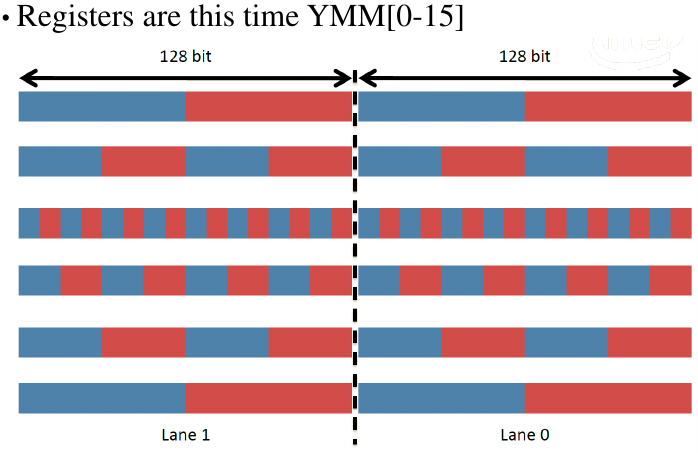
\includegraphics[scale=0.5]{immagini/sse_lanes.png}
\end{figure}
\subsection{Allineamento della memoria}
Alcune delle operazioni che portano dati nei registri lo fanno in maniera corretta solo se l'indirizzo è allineato a certi vincoli, possono esserci vincoli di allineamento ad 8 o 16 byte e questo è importante perché se viene chiamato un intrinsic di gcc che usa una di queste istruzioni può essere necessario avere allineamento di memoria. Abbiamo visto che è possibile in C avere aree di memoria già allineate (vedi istruzioni sopra).\\ Ci sono diversi instrinsics gcc da chiamare per poter usare i registri vettorizzati:
\begin{figure}[!h]
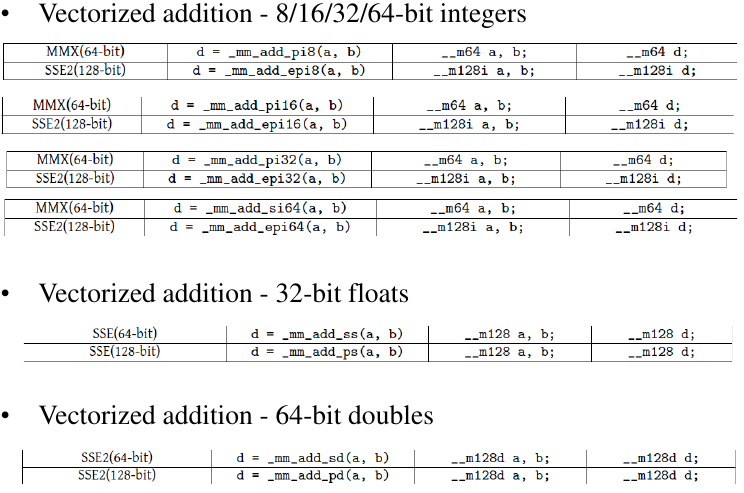
\includegraphics[scale=0.5]{immagini/sse_gcc_intrinsics.png}
\end{figure}

\chapter{Kernel programming basics}
\section{Addressing}
\subsection{Linear addressing}
Vediamo le modalità con cui si fa addressing di dati ed istruzioni. Una delle modalità più interessanti che ci sono è il linear addressing, in cui le informazioni usabili dal processore sono viste come una sequenza lineare, quando esprimiamo un indirizzo l'unica cosa da specificare è un offset, ovvero il punto dove collocarsi con l'operazione di lettura/scrittura. L'indirizzamento è di memoria, magari anche di memoria fisica, oppure di memoria logica, per cui distingueremo indirizzamento fisico e logico.\\ Quello che realmente accade in architetture moderne e che si usano anche altri concetti, tra cui la segmentazione
\subsection{Segmentazione}
Abbiamo un address space in cui il processore può leggere/scrivere. Potremmo identificare delle zone differenti, che sono magari indirizzabili non solo tramite offset, ma esprimendo un segment\_id + offset, quindi l'offset è interno allo specifico segmento. In un sistema moderno si combinano i due approcci: si dice che si vuole accedere ad un segmento specifico, ma poi l'accesso al singolo segmento viene tradotto come offset in una zona lineare: quindi possiamo avere questo tipo di collocazione:
\begin{figure}[!h]
	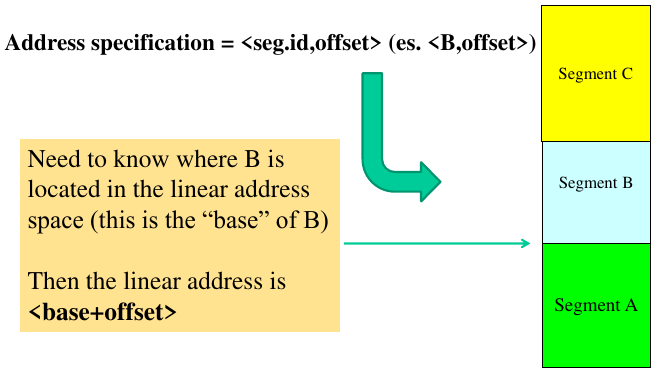
\includegraphics[scale=0.3]{immagini/la_seg.png}
\end{figure}
l'accesso a B va tradotto nel calcolo assoluto dell'offset all'interno dell'address space lineare. Il punto nodale è che quando esprimiamo un indirizzo per toccare delle informazioni, questo passa per la nozione della base del segmento a cui si vuole accedere, perché l'indirizzo sarà dato dalla base + l'offset a cui si vuole accedere. Ricordiamo che la memoria può essere sia fisica che logica, quindi abbiamo o non abbiamo il passaggio in più, legato al concetto di memoria virtuale
\subsection{Memoria virtuale}
Se siamo in memoria logica, vogliamo prendere un indirizzo lineare ed accedere alla zona di memoria, ma non sappiamo se è in memoria e dove è in memoria fisica. Quindi il passaggio in più è presente o meno a seconda dell'hardware e del software che si utilizza, come riassunto di seguito:
\begin{figure}[!h]
	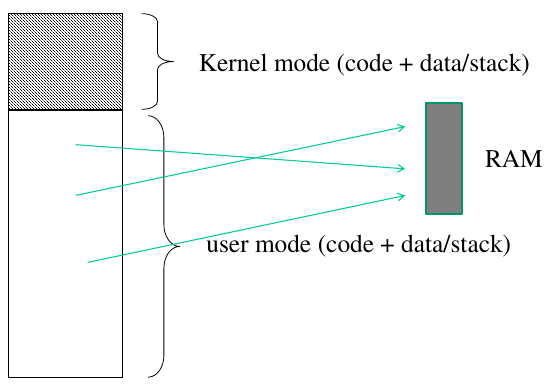
\includegraphics[scale=0.3]{immagini/vm.png}
\end{figure}
In ogni caso, quello che il processore deve fare è: indirizzo segmentato $\rightarrow$ indirizzo lineare $\rightarrow$ indirizzo nella pagina $\rightarrow$ indirizzo fisico. Abbiamo il supporto per eseguire la traduzione e la traslazione degli indirizzi in maniera efficiente, e questo vuol dire anche capire se l'accesso in memoria che si sta cerando di risolvere è plausibile in quel momento o no, in termini dei privilegi che il processore ha in quel momento. Esempio in x86:
\textsf{mov (\%rax), \%rbx}, \textsf{push \%rbx}, qui stiamo usando 3 segmenti differenti, non li usa chi ha scritto il programma, bensì il processore in maniera autonoma si rende conto che le operazioni stanno toccando diverse zone di memoria: i due segmenti sono dati dagli indirizzi di \%rax, dal fatto che si fa la push di \%rbx, il terzo è dato da dove sono le istruzioni. Il processore sta eseguendo il fetch delle istruzioni, che è un accesso in memoria e quindi passa tramite le regole dette sopra.
\subsection{Processori di sistema e segmentazione}
I processori di sistema sono quelli per cui pensiamo di eseguire codice di SO, qui il supporto per eseguire la traslazione e validarli è dato da un'insieme di informazioni tipicamente mantenuti in un insieme di registri o tabelle di memoria, il che vuol dire che oltre alla page table servono anche altre informazioni per accedere alla memoria che sono interni ad altri componenti e sono:
\begin{itemize}
\item registri di CPU
\item tabelle in memoria, puntate direttamente dai registri
\end{itemize}
Sui processori moderni ci si muove sia con la segmentazione che con gli indirizzi lineari, quindi si esprime un indirizzo segmentato che viene traslato in lineare etc... come sopra, quindi tutti i passaggi hanno bisogno delle informazioni che vengono inserite in registri e tabelle: tipicamente lavoriamo con la page table, per cui se abbiamo un indirizzo lineare, possiamo paginarlo ed associarli un indirizzo fisico. Per avere una traslazione di indirizzo segmentato a lineare possiamo avere la seguente traduzione in hadware:
\begin{figure}[!h]
	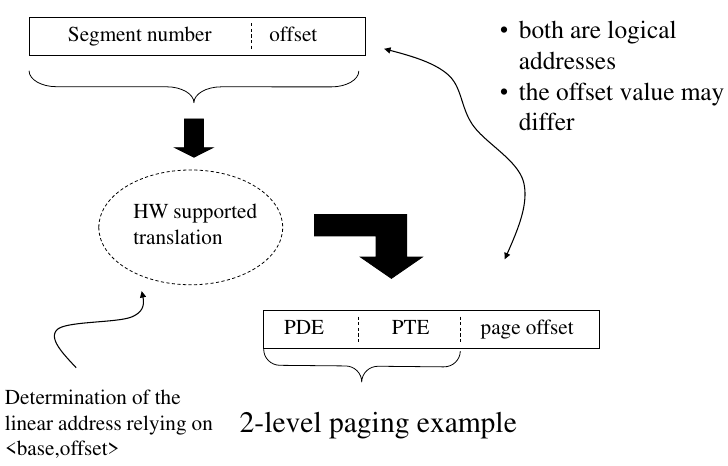
\includegraphics[scale=0.3]{immagini/seg_pag.png}
\end{figure}
\\ Consideriamo qualcosa in più, il concetto del segment selector
\subsubsection{Segment selector}
Quando si usa un indirizzo segmentato, viene specificato il registro del segment selector, quindi non il nome del registro bensì il nome del segment selector. Il registro contiene le informazioni sul segmento che si vuole prendere, quindi abbiamo il seguente schema:
\begin{figure}[!h]
	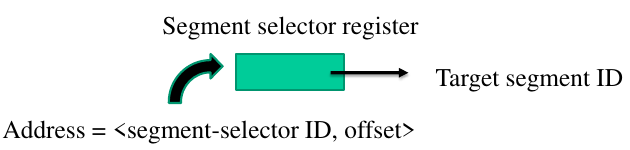
\includegraphics[scale=0.3]{immagini/seg_sel.png}
\end{figure}
se abbiamo una istruzione macchina per accedere ad uno specifico segmento in memoria, per poi in futuro accedere ad un altro, è possibile usare sempre la stessa istruzione e basta specificare il registro di segmentazione corretto. Il caso classico è se il codice viene eseguito su un thread piuttosto che un altro: il codice macchina è identico, che però tocca segmenti differenti usando questo tipo di meccanismo.
\section{Accesso in memoria su x86}
Abbiamo il real mode x86, un po' datato, protected mode ed il long mode (variante più recente). Vediamo l'x86 real mode 
\begin{itemize}
\item segment register a 16 bit, ce ne sono 4
\item registri a 16 bit generali per gli offset. Possiamo specificare in una istruzione dove richiediamo di accedere alla memoria dove punta quel registro, che può essere un puntatore
\end{itemize}
L'indirizzo fisico a cui accediamo è calcolato come: \texttt{Segment}*16+\texttt{Offset}. Possiamo accedere a circa 1 MB di memoria, la cosa interessante è che nei registri non si mantenevano informazioni riguardo alla protezione, quindi la macchina non era adeguata per implementare software di sistema, perché non c'è la nozione di protezione, quindi nemmeno software relativo alla VM. Tutto ciò che esegue può usare questo schema.
\subsection{x86 protected mode}
Abbiamo le seguenti caratteristiche:
\begin{itemize}
\item registri a 16 bit per tenere i segment ID, usiamo solo 13 bit per specificare gli ID, con gli altri specifichiamo delle caratteristiche relative ai privilegi: un certo segmento può essere toccabile solo se si lavora ad un certo livello di privilegi
\item registri general purpose a 32 bit, usati come pointer e che puntano nel segmento 
\end{itemize}
quando vogliamo toccare un certo segmento, ci chiediamo quale è la base nell'indirizzamento collocato e quale è il suo offset: l'ID del segmento nel registro segmentato è un indice della tabella, che contiene la base del segmento e quindi avremo che gli indirizzi che otteniamo sono lineari: \texttt{address} = \texttt{TABLE[segment].base + offset}. Possiamo quindi identificare l'offset assoluto nella memoria per poter leggere e scrivere, essendo i registri degli offset a 32 bit, possiamo indicizzare 4GB. I 3 bit non usati possono essere impiegati per la protezione, quindi l'istruzione permette di toccare determinate zone di memoria in base alle determinate configurazioni
\subsection{Long mode x64\_64}
È una estensione del precedente
\begin{itemize}
\item segment registers a 16 bit, di cui ne usiamo sempre 13
\item registri general purpose a 64 bit per usare gli offset per accedere in memoria. Se usiamo lo stesso meccanismo di prima, è tutto a 64 bit e quindi possiamo avere $2^{64}$ come offset nello spazio lineare. Ma non è così, abbiamo solo 48 bit disponibili: preso un registro come \texttt{rax}, mettiamo una bitmask che esprime un offset per accedere alla memoria, possiamo scrivere i 64 bit come vogliamo, ma quando passiamo questo all'interfaccia per l'accesso alla memoria, vengono scartati i bit più significativi e se ne usano solo 48 (gli altri sono settati a valori di default).
\end{itemize}
Qui possiamo indicizzare 256 TB di memoria lineare.
\subsection{Tabella di segmentazione}
In x86, quando abbiamo un segment selector, abbiamo un ID e le tabelle considerate possono essere 2 per ogni flusso di esecuzione
\begin{itemize}
\item GTD
\item LDT
\end{itemize}
possiamo specificare se l'indice è riferita all'una o l'altra tabella, mediante l'utilizzo di un apposito bit di controllo che specifica quale tabella considerare. In sistemi moderni, si considera solo la GDT, che ad ogni istante di tempo dice, dato un thread in esercizio sulla CPU, esattamente ogni segmento toccabile dai selettori dei registri usati dal thread. La GDT indicava qualcosa di globale, nel senso che venivano indicate anche informazioni riguardo la base del segmento accessibile a livello kernel, ma questa informazione valeva per tutti i thread. La struttura della GDT è la seguente
\begin{figure}[!h]
	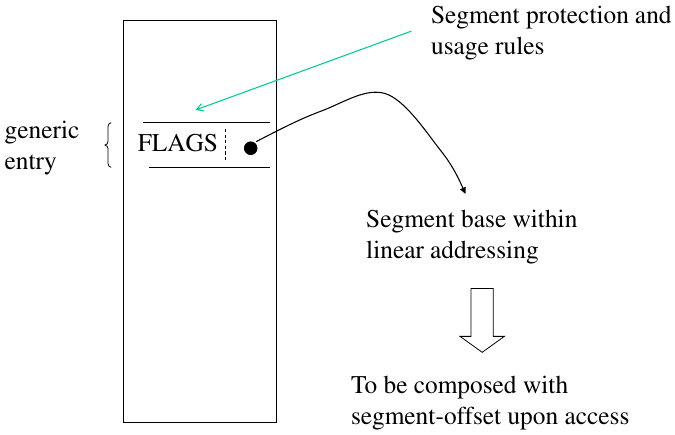
\includegraphics[scale=0.3]{immagini/gdt_table.png}
\end{figure}
in una entry, oltre alla base del segmento, ci sono anche flags addizionali per gestire correttamente il segmento. Sappiamo come accedere al segmento, i flags specificano cosa si può fare con quel segmento.
\subsection{Segmentazione e paginazione}
Nella GDT ci sono informazioni per la gestione del segmento, ma da un indirizzo lineare si passa ad uno fisico e c'è la tabella delle pagine che ha anche essa dei bit di protezione, sappiamo se il frame che tocchiamo è di livello kernel o user. Quindi perché c'è questo overload nel meccanismo di protezione, inoltre perché è presente anche la segmentazione nonostante la paginazione gestisce la memoria. La paginazione è un modo per gestire la memoria a grana molto fine, mentre la segmentazione è a grana molto più grande: potremmo avere un address space lineare fatto da un unico segmento $s_0$, quindi la protezione per il segmento è per l'intero address space, diverso da quelle che potrei avere per le singole pagine nella page table.\\ Inoltre, l'architettura per cui abbiamo la segmentazione per accedere alla memoria è stata estesa perché con la segmentazione data una istruzione macchina correntemente in esecuzione sulla CPU, è possibile che il thread ad un certo istante di tempo tocca lo spazio lineare da una certa parte, mentre l'istruzione per un altro thread tocca l'address space lineare da un'altra parte. I thread possono girare su diverse CPU se abbiamo TLP, quindi eseguire delle istruzioni macchina identiche ma toccando diverse zone di memoria, quindi possiamo gestire la memoria segmentata in maniera più modulare di come faremmo con la paginazione, quindi è la base del multi-threading e del multi-coring:
\begin{itemize}
\item Thread Local Storage
\item Per-CPU memory
\end{itemize}
Nella segmentazione, la grana di protezione è più grossa in quanto con pochi bit si può andare a definire cosa fare anche su un intera area di memoria, ma è utile sopratutto quando si lavora con TLP, quindi in maniera concorrente, inoltre la segmentazione è stata portata avanti quando la paginazione era già supportata dai sistemi.\\ Scendiamo nel dettaglio della protezione della segmentazione
\subsection{Protezione nella segmentazione}
Possiamo associare a ciascun segmento un certo livello di protezione. Ragioniamo sulle variazioni di flusso di esecuzione, ma gli stessi concetti valgono anche per l'accesso ai dati, ogni routine che ha un livello di protezione \texttt{h} in uno schema di protezione basato su segmentazione può invocare qualunque altra routine, che può essere anche in un altro segmento, di livello \texttt{h}. Quindi, i salti possono essere intra-segment ma anche cross-segment, ma occorre che il livello di protezione della sorgente e del target siano allo stesso livello di protezione. Possiamo anche muoverci con valori differenti di protezione, dobbiamo sicuramente avere un salto cross-segment, perché se fossimo nello stesso segmento si avrebbe lo stesso livello, è sempre possibile saltare al livello \texttt{h+i}, se questo è il livello target, si passa ad una routine meno privilegiata.
\subsubsection{Protection GATEs} 
Abbiamo che ogni segmento ad un livello di protezione \texttt{h} è  associato con un insieme di access points, detti \textbf{GATEs}, ognuno identificato con una coppia $<$\texttt{seg.id},\texttt{offset}$>$ ed ogni GATE ha associati un livello massimo \texttt{max = h+j} da cui è possibile saltare.\\ Quindi il passaggio a livello superiore si può fare solo se la prima istruzione macchina della routine è un così detto \textbf{GATE di accesso}.\\Passare per il GATE vuol dire che non si possono usare le stesse istruzioni macchina che si eseguivano per saltare nello stesso segmento, i GATE sono porte di accesso che permettono di "entrare e diventare più privilegiato", ma non è ammesso a qualunque thread, bensì ad un massimo livello di privilegio ammissibile per passare nel GATE.\\ Quindi, se il livello di un certo segmento \texttt{S} è pari ad \texttt{h}, ed il \texttt{max(GATE(S)) = h+i}, allora il segmento \texttt{S} ha un GATE che permette l'accesso ai moduli che hanno un livello di protezione da \texttt{h+i} in su.\\Il modello basato su segmentazione implementa un \textbf{ring model}:
\begin{figure}[!h]
	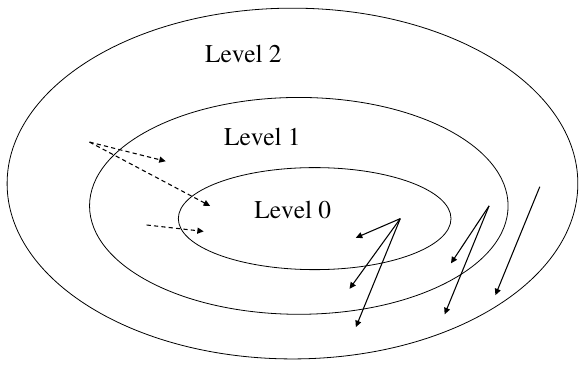
\includegraphics[scale=0.3]{immagini/ring_model.png}
\end{figure}
eventualmente si salta da 0 in avanti in dei target che hanno dei livelli di protezione peggiori o pari a chi salta, mentre per fare il contrario dipende dal GATE. Abbiamo quindi un address space lineare, fatto da zone che sono dei segmenti e possiamo avere segmenti livello user o kernel:
\begin{figure}[!h]
	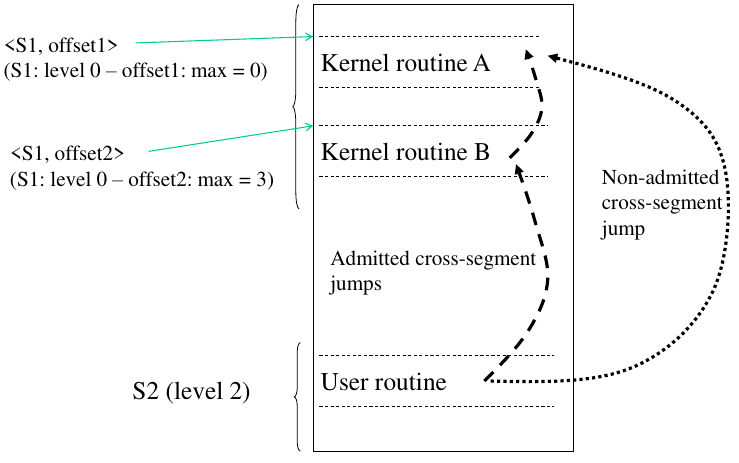
\includegraphics[scale=0.3]{immagini/routine_priv.png}
\end{figure}
abbiamo 3 routine, una user e due kernel, le due istruzioni kernel sono GATE:
\begin{itemize}
\item nel GATE \texttt{kernel routine A} si permette il passaggio solo intra-segment;
\item il GATE \texttt{kernel routine B} ha un max pari a 3, quindi ad esempio provenendo dal GATE del livello S2 si può saltare nel segmento a livello di privilegio B, ed a quel punto chiamare il GATE di A
\end{itemize}
Possiamo perciò comporre in un address space non solo il meccanismo della paginazione, che ci dice che i segmenti sono kernel, ma la segmentazione offre supporto in più per avere questo passaggio che permette di usare davvero quello che è presente nel segmento kernel.\\ Quindi gli obiettivi della segmentazione sono offrire delle protezioni ulteriori rispetto a quelli della paginazione, inoltre permette di cominciare a fare qualcosa in un livello di protezione maggiore: in uno SO abbiamo un interrupt, magari mentre eseguiamo software di livello user ad un certo istante t, per processare le attività associate all'interrupt che sono magari cablate in attività lato kernel, occorre passare a privilegi lato kernel; quindi, per ogni interrupt deve essere definito un GATE, altrimenti non è possibile gestire l'interrupt.\\ 
(((Quando viene chiamata una syscall abbiamo un oggetto machine-dependent del tutto generale chiamato dispatcher, in grado in funzione del fatto che è stata chiamata una syscall e quindi una trap, di leggere il valore eventualmente scritto in un registro e capire dove redirigere il flusso di esecuzione nel codice kernel.)))\\Abbiamo quindi interrupt e GATEs, con cui permettiamo a software di livello user di eseguire attività necessarie.
\subsection{Ring model in x86}
Lo schema ad anello dell'x86 è fatto nel seguente modo:
\begin{figure}[!h]
	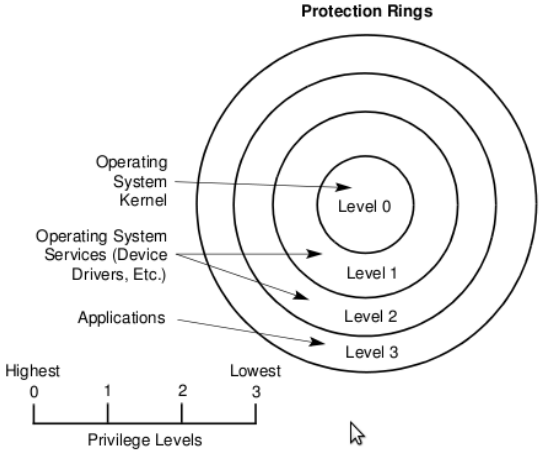
\includegraphics[scale=0.3]{immagini/ring_x86.png}
\end{figure}
servono quindi, per discriminare il livello di protezione, 4 bit in quanto abbiamo 4 livelli diversi di protezione.\\A livello 0, all'interno di una architettura segmentata abbiamo tutte le informazioni del kernel: possiamo fare qualsiasi cosa, ovvero toccare qualsiasi altra informazione anche a livello user.\\ Tipicamente le applicazioni user girano a livello 3, i due livelli intermedi inizialmente non erano nemmeno usati, man mano sono stati usati per implementare servizi di sistema, ad esempio per la schedulazione delle VM.\\ Quando facciamo qualsiasi accesso in memoria, si va a specificare il segment seletor register ed eventualmente un displacement, in modo che riprogrammando il registro per attività in tempi differenti, andremo in diverse aree di memoria. Vediamo quanti e quali selettori di segmenti ci sono
\subsubsection{Registri di segmento}
Il registro di segmento ha informazioni sia sul nome del segmento, sia informazioni sulla protezione del segmento (16: 13 $|$ 3).\\ Su x86 l'utilizzo comune prevede solo la GDT, ma c'è comunque un bit che dice dove andare a prendere il segmento, abbiamo poi altre informazioni di protezione. I selettori di segmento sono 6, i primi 4 erano quelli originali e gli altri due sono stati aggiunti, quindi la segmentazione è andata avanti a prescindere dalla paginazione
\begin{itemize}
\item CS: si stabilisce in un address space quale è la zona dove è presente il codice di cui fare i fetch. Discriminiamo cosa è usabile dal punto di vista di esecuzione del processore, il registro viene ad esempio usato proprio dal processore quando deve andare all'istruzione successiva
\item SS: in che zona dell'address space è posizionata la zona di stack. Viene usato quando si fanno push e pop
\item DS ed ES: segmenti dati, usabili per accedere ai dati delimitandone la posizione nel segmento specifico
\item FS e GS: aggiunti dopo nell'80386
\end{itemize}
Quando lavoriamo su CS, i 2 bit RPL sono anche detti CPL ovvero il Current Privilege Level, quindi quale è la capability del processo in esecuzione.\\ Analizziamo uno snippet visto in precedenza, possiamo capire quali sono i registri di segmento usati:
\begin{lstlisting}
mov (%rax), %rbx
push %rbx
\end{lstlisting}
Abbiamo un offset all'interno del code segment, perché usiamo il PC per fetchare le istruzioni che è un offset, la base è dato dal CS. Il DS è un offset per accedere alla memoria, il pointer di default dice dove acquisire il dato. La push utilizza l'offset per capire dove andare in memoria, quindi usa il registro SS. ES viene usato al posto di DS quando si eseguono delle istruzioni particolari, ad esempio quelle string-targeted come \textsf{stos} e \textsf{movs}
\subsection{GDT di x86}
La tabella fondamentale che contiene le informazioni sul fatto che dato che qualcuno sta facendo una istruzione che deve fare qualcosa, dice quel qualcosa dove è in memoria. Questa è una entry della tabella:
\begin{figure}[!h]
	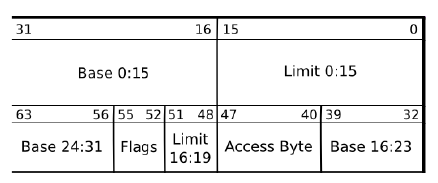
\includegraphics[scale=0.5]{immagini/gdt_entry.png}
\end{figure}
ciascuna entry da informazioni sul segmento associato a quell'indice. La tabella è fondamentale, perché il registro può essere cambiato e quindi anche l'informazione per il segmento di indice i va salvato, altrimenti non saprei come recuperarne le informazioni.\\ La tabella ha 8 byte usabili per un processore ad 32 bit, manteniamo
\begin{itemize}
\item base 0:15
\item base 24:31
\item base 16:23
\end{itemize}
tutte le altre informazioni sono di controllo
\begin{itemize}
\item access byte: dice se la entry è valida o no
\item limite, dice al  più quanto è ampio il segmento, quindi quale è il massimo offset per accedere, può avere diverse taglie (in base al valore limit 16:19???)
\end{itemize}
Il privilege level viene caricato in un registro di processore quando vogliamo usare un segmento nel programma.
\subsubsection{Accesso alla GDT}
Se vogliamo accedere ad un segmento e caricare le informazioni su quel segmento, come fa il processore a sapere dove è in memoria quel segmento: c'è un registro apposito che è il \textbf{gdtr}, puntatore che porta all'interno della memoria per sapere dove è posizionata la GDT. È un puntatore, quindi un offset ma rispetto a quale memoria? Stiamo cerando di identificare nella memoria alcune informazioni basiche per gestire la memoria segmentata, quindi è in memoria lineare. L'organizzazione è la seguente:

È interessante che gdtr si può leggere anche a livello di privilegio 3, magari non si riesce ad accedere a quel punto della memoria, perché magari è in un segmento non accessibile a livello 3.\\ Quando leggiamo il registro, in realtà abbiamo una informazione packed
\begin{itemize}
\item l'indirizzo del registro
\item il numero di entry che la tabella ha correntemente
\end{itemize}
mettiamo le informazioni in una struttura packed, usando la API \texttt{store\_gdt}, che è codice asm volatile che non fa altro che prendere sgdt e mette il valore nel puntatore. La chiamiamo due volte, passando due parametri differenti, in un caso un array di byte.
\begin{lstlisting}
#define store_gdt(ptr) asm volatile("sgdt %0":"=m"(*ptr))
\end{lstlisting}
è possibile, anche se con scarsa probabilità, che abbiano diversi valori, ma la si può aumentare chiamando un servizio bloccante come la sleep.\\Se l'applicazione venisse schedulata e poi reschedulata su un'altra CPU, avremmo trovato dei valori di GDT differenti\\\\ A 64 bit abbiamo che la taglia delle entry è il doppio,  manteniamo alcune informazioni 
\begin{figure}[!h]
	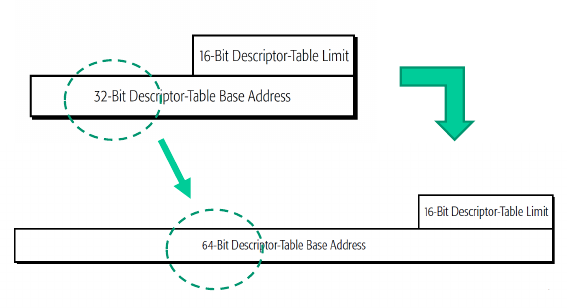
\includegraphics[scale=0.5]{immagini/64bit_gdtr_entry.png}
\end{figure}
Supponiamo di voler usare un selettore di segmento, avendo anche l'indice, sarebbe importante sapere l'offset del segmento perché altrimenti non potremmo fare tutti gli altri passaggi. Sappiamo che è nella GDT, accediamo con un selettore di segmento, accediamo ad un offset, viene  mostrato in seguito uno schema
\begin{figure}[!h]
	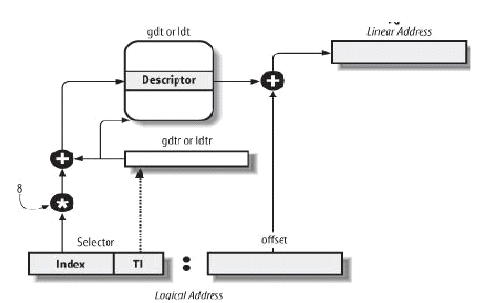
\includegraphics[scale=0.5]{immagini/accesso_gdt.png}
\end{figure}
Su x86, quando abbiamo un segment selector, invece di andare sempre in memoria l'informazione viene cachata in una zona apposita quando abbiamo già il selettore, l'aggiornamento di un selettore prevede che si vada in tabella, si prenda il selettore e si metta l'informazione in una cache interna al processore:
\begin{lstlisting}
#include <stdio.h>

#define load(prt, var) asm volatile("mov %%ds:(%0), %%rax":"=a"  (var):"a" (ptr))
#define store(val, ptr) asm volatile(" mov %0, %%ds:(%1)" ::"a" (val);
"b" (ptr):)

int main(int argc, char **argv){
	unsigned long x = 16;
	unsigned long y;
	
	load(&x, y);
	printf("variable y has value %u\n", y);
	
	store(y+1, &x);
	printf("variable x has value %u\n", x);
}

\end{lstlisting}
Quello che capiamo è che andando a toccare i diversi dati, questi possono essere mappati sullo stesso segmento.
\subsection{Code e data segment per Linux}
Vediamo come Linux configura la GDT usata da uno dei processori per capire dove sono posizionati i segmenti: ci sono 4 entry nella GDT usate da Linux
\begin{figure}[!h]
	\includegraphics[scale=0.5]{immagini/tabella_gdt.png}
\end{figure}
\begin{itemize}
\item user code: la entry tiene traccia di qual è la posizione del segmento dove ci sono istruzioni utente, la base è 0
\item user data: la posizione ha sempre base 0, quindi se usiamo un offset specificando questo segmento o quello precedente arriviamo nella stessa area di memoria
\item kernel code: le informazioni che costituiscono la parte eseguibile del kernel è sempre a partire da base 0
\item kernel data: base 0 anche per lui
\end{itemize}
Se ragioniamo su cosa realmente accade, è che presi questi 4 segmenti di base, all'interno dell'address space questi sono sovrapposti, partono tutti dalla stessa base 0. Se abbiamo un offset per identificare un dato o una istruzione, in realtà questo è un offset assoluto, si identifica in maniera univoca una posizione nell'address space. La segmentazione resta fondamentale quando vanno gestiti i GATE, altrimenti non potremmo stabilire se, indipendentemente da come il processore raggiunge le cose nell'address space, è possibile prendere o meno il GATE.\\La scelta di usare al minimo la segmentazione nello sviluppo del kernel Linux: abbiamo un insieme di moduli che rappresentano il kernel Linux, la scelta di mappare a 0 tutti i 4 segmenti nativi è che, se supponiamo che i concetti di segmentazione sono sparsi ovunque nel kernel, quindi prendere il kernel e ridisegnarlo per portarlo su una macchina dove la segmentazione non c'è vuol dire riscrivere un kernel diverso. Altra cosa è se la segmentazione viene configurata in modo che l'offset è assoluto, viene ridotto l'impatto della segmentazione alle poche parti segmentation dependent, in modo da far si che è semplice portare il kernel per eseguirlo su macchine che usano la segmentazione. Ma se bisogna riscrivere il TLS in una architettura dove la segmentazione non c'è, va riscritto poco codice perché quello già esistente è molto portabile.
\subsubsection{Versione a 64 bit, long mode}
Nel long mode, ovvero x86\_64, i vendor hanno fatto sì che per tenere traccia del segment ID, per alcuni selettori di segmento la base è per default settata a 0, quindi l'offset è assoluto.\\Per 4 dei selettori vale questo, per gli altri 2 vale ancora che la base associata al segmento va presa dalla tabella. Quindi per alcuni selettori si può accedere direttamente senza passare per la tabella, ma non per tutti altrimenti si perde la capacità di poter costruire software sfruttando la segmentazione, comunque questa scelta permette di accedere rapidamente ai segmenti discriminando solo aspetti di protezione, ma anche poter usare dei segment selector che vanno in due zone diverse nello stesso flusso di esecuzione.
\subsection{Gestione dei selettori in x86}
Se i segmenti non servono più a discriminare dove lavoriamo, perché sono tutti mappati a 0, il code segment rimane importante perché c'è il CPL: se è targato con CLP = 00, stiamo lavorando in qualche segmento di codice a livello kernel, se è 11 stiamo lavorando in qualche segmento user dove non è vero che tutto è permesso.\\Questo ci mette già di fronte all'idea che una stessa istruzione macchina dell'ISA viene eseguita in diversi casi di valori di CPL e che possiamo avere diversi risultati, quindi il CPL al di là di dove sono posizionate le cose in memoria permette di distinguere diverse modalità operative.\\ È possibile aggiornare CS? No, l'unico modo per cui avviene il cambiamento del CPL (se siamo su x86\_64 conta solo questo) è solo quando abbiamo dei control flow particolari. Una delle cause per generare queste conseguenze è il passaggio per un GATE, l'istruzione che fa passare nel GATE aggiorna il CPL, ovviamente quando CPL=0 ed è tutto lecito.\\ Tutti gli altri selettori di segmento possono essere aggiornati se il segment descriptor a cui sono associati ha DPL $\geq$ CPL corrente
\subsection{GDT estesa in Linux}
La GDT classica di Linux è la seguente:
\begin{figure}[!h]
	\includegraphics[scale=0.3]{immagini/linux_gdt.png}
\end{figure}
alcune entry indicano dove in un address space lineare vengono posizionati i dati kernel/user, ma gli offset che ci dicono dove sono posizionati i segmenti portano sempre a 0, quindi l'offset è assoluto. La segmentazione gioca un ruolo solo nei termini della protezione, vediamo inoltre che tra i segmenti interessanti c'è il \textbf{TSS}: è un segmento posizionato nell'address space a base diversa da 0 e se consideriamo un address space lineare abbiamo che data l'esistenza sulla macchina della CPU x, c'è una zona associata alla specifica CPU x, stesso vale per le altre CPU. I TSS sono queste zone "riservate", quindi esiste un segmento nell'address space lineare posizionato ad una base differente per ogni CPU (o hyperthread fisico).\\ Nel TSS ci sono informazioni basiche per tenere traccia, mentre su una certa CPU che esegue uno specifico thread, le cose relative al ring model, quindi come l'oggetto si muove nel ring model.
\subsection{TSS (Task State Segment)}
Il TSS era tale per cui l'oggetto era una collezione di informazioni, raggruppati in un array ed ogni array aveva un'associazione con lo specifico CPU core. Questo array aveva una certa taglia, un certo valore dei bit di protezione, è quindi un informazione accessibile a livello kernel, TSS da lo stato del task in esercizio sulla CPU. Internamente, su x86 ad esempio, abbiamo la seguente struttura:
\begin{figure}[!h]
	\includegraphics[scale=0.3]{immagini/linux_gdt.png}
\end{figure}
salendo nelle informazioni, troviamo locazioni di memoria che tengono traccia dei registri del processore. Potremmo installare nella zona uno snapshot del processore, ma anche informazioni di segmentazione che il processore sta usando, quindi tutta la fotografia del processore.\\ Inizialmente, era stato pensato per implementare il context switch a livello hardware, quindi con apposite istruzioni macchina.\\ Le zone ESP sono Extended Stack Pointer, quindi registriamo 3 stack pointers differenti, ma il processore ha un solo ESP: i 3 diversi stack poninter servono per avere nella specifica zona quali sono le capability del thread in ring model, così che sappiamo che se cambia il livello di privilegio, magari dobbiamo usare una stack area differente. La struttura viene usata anche dal firmware, il ring model = utilizzo eventualmente i GATE, quindi istruzioni macchina per cui il processore potrebbe dover cambiare priorità. Tutta la parte sopra è inutile, perché l'oggetto non è usato per implementare context switch hardware, su Linux è basato su software e quindi la zona sotto è stata espansa per ospitare stack pointer a 64 bit e poter avere nell'area una rappresentazione corretta delle informazioni che rappresentano il ring model. Quando arriva un interrupt, ed il thread che esegue deve cominciare ad eseguire una routine del kernel, va cambiato livello di priorità ed in particolare una stack area differente per poter far lavorare l'handler.
\subsubsection{Come arrivare al TSS}
Per arrivare al TSS si può usare la GDT, ma il processore vorrebbe cercare di eseguire un numero di accessi in memoria ridotto per poter usare un oggetto così importante. Quindi, in x86 abbiamo un registro di processore, il TSS register che può essere usato con l'istruzione \texttt{LTR}, con cui possiamo fare questa operazione:
\begin{itemize}
\item carichiamo un elemento della GDT con un certo ID;
\item quando viene caricata l'informazione, viene anche eseguito altro dal processore, ovvero l'analisi del contenuto dell'informazione per determinare la base di dove in memoria è la GDT;
\item la base viene caricata nel TSS register, quindi l'informazione è packed
\end{itemize}
il processore può controllare in maniera efficace il thread, se va cambiato stack ha la base del segmento.
\subsection{Replicazione della GDT}
Nella tabella c'è una entry dove c'è il TSS, ma se abbiamo più CPU come teniamo traccia di più di un segmento con una sola entry per TSS? I due processori hanno due TSS diversi, dove identifichiamo la base per i due TSS? Quando lavoriamo con la segmentazione su un architettura di SO moderno, seguiamo uno schema con GDT replicata, abbiamo differenti GDT per i diversi processori in esecuzione. Possiamo avere 2 diversi processori $CPU_0$ e $CPU_1$ che hanno due GDT diverse, e se queste sono popolate differentemente, i due CPU core stanno usando degli indirizzi logici differenti sullo spazio degli indirizzi lineare.\\ I motivi di esistenza della GDT replicata sono
\begin{itemize}
\item flessibilità
\item trasparenza quando i diversi processori accedono in memoria
\item performance: le tabelle vengono messe su nodi NUMA, se sono vicini alle CPU core non interferiscono fra loro
\end{itemize}
replicando si evita anche di scrivere cose all'interno del software, in modo da poter girare lo stesso in maniera agnostica rispetto al CPU core dove gira.\\ Uno schema può essere il seguente:
\begin{figure}[!h]
	\includegraphics[scale=0.4]{immagini/gdtr_schema1.png}
\end{figure}
le tabelle possono essere identiche, quindi le due CPU vedono gli stessi indirizzi e quindi vanno negli stessi punti di memoria oppure avere alcuni punti differenti, questo mappa su cosa fa il software: supponiamo di usare il selettore di segmento GS, se abbiamo caricato una entry piuttosto che un'altra, usando GS sulle diverse CPU core si va in punti differenti della memoria perché cambiano le basi.
\begin{figure}[!h]
	\includegraphics[scale=0.4]{immagini/gdtr_schema2.png}
\end{figure}
questo è stato ampiamente sfruttato nei SO, perché è classico che ci siano informazioni importanti per la specifica CPU ad uno specifico intervallo di tempo. Devono stare in memoria ed il problema è ritrovarla la memoria: se non ci fosse questo meccanismo, dovrebbe essere la CPU stessa a chiedersi chi è lei, per andare nell'array che contiene le gdtr per toccare la zona designata e questo sarebbe devastante per le architetture moderne, CPUID squasha la pipeline quindi costa. Il meccanismo permette di implementare la \textbf{per CPU memory}, la CPU arriva in automatico alla zona di memoria associata alla specifica CPU.\\Nei kernel dei SO è esteso ampiamente, vengono messe delle informazioni base riguardo ciò che deve accadere per una specifica CPU. È interessante per fare cose come la \textbf{statistics update}:
\begin{itemize}
\item se le statistiche sulla CPU sono globali, servono istruzioni atomiche;
\item per-CPU memory: aggiorno le informazioni nella specifica zona
\end{itemize}
\subsubsection{Gestione della per-CPU memory in Linux}
Allo startup, viene identificata per ogni CPU attiva una specifica zona di memoria. Lì, vanno inserite tutte le variabili di interesse, l'oggetto di memoria viene identificato tramite lo specifico selettore di segmento, che è GS. Quando viene scritto codice del kernel, possiamo sfruttare la per-CPU memory con delle macro apposite, con la \texttt{DEFINE\_PER\_CPU(tipo variabile, nome variabile)}, per accedere alla variabile o si usa un'altra macro, ad esempio per ottenere x in un altro registro oppure usare una API che prende il puntatore alla variabile e calcola, dalla variabile, la sua posizione in memoria, vi somma la base e restituisce l'offset assoluto ed è possibile andare in memoria anche tramite gs. Tutto questo è trasparente ed è data dal fatto che abbiamo per-CPU memory e replicazione della GDT, viene eseguito con la seguente istruzione:\\
\texttt{mov ax, gs:[x]}.
\subsection{Thread Local Storage}
Equivalente alla per-CPU memory, per ottenerlo usiamo la segmentazione: c'è una zona della tabella in cui si possono usare delle entry per gestire il TLS. Le entry identificano dei segmenti, quindi delle posizioni in memoria, a livello kernel quando decidiamo di schedulare un thread in CPU, possiamo cambiare il contenuto della tabella postando nelle entry informazioni che vogliamo, in modo che la visione del thread siano "personalizzate" per il sinoglo thread.\\ Usando FS, possiamo caricare una delle entry quando decidiamo di schedulare il thread, identifichiamo in FS la base in memoria del TLS. Il TLS di gcc permette di usare una sola di queste zone, allo startup il thread chiede di usare una di quelle zone e di metterla in FS, avendone 3 possiamo fare cose "più spinte", vediamo come.\\ La syscall è \texttt{arch\_prctl}, che ha diverse nomenclature: si passa il controllo al kernel internamente, cosa fare viene specificato nel \texttt{code}, passano il parametro.\\ Nella prima signature della funzione, si passa il codice ed un \texttt{unsigned long}, quindi possiamo identificare un offset dell'address space lineare, quindi indichiamo probabilmente una base in cui va caricato un segmento. Vogliamo quindi che per un segmento specifico utilizzare una specifica base.\\A livello kernel, viene messo in una delle entry TLS e viene riflesso il valore aggiornato nel registro di segmentazione, quindi quel thread userà una specifica area. L'area di memoria deve essere stata allocata, quindi ad esempio con una \texttt{mmap}, per poi fare il setup livello kernel.\\ Possiamo fare anche una query, otteniamo la base del segmento quando il thread corrente va in CPU.
\section{Internals di x86}
\subsection{Registri di controllo x86}
Ci sono 3 o 4 registri di controllo di x86, targati con CR*
\begin{itemize}
\item CR0 è un registro di controllo baseline, servono al processore per capire come comportarsi quando accadono determinate cose;
\item CR1 è riservato;
\item CR2 mantiene l'indirizzo lineare quando abbiamo un fault;
\item CR3 è il page table pointer, quindi il posizionamento in memoria fisica della page table corrente;
\end{itemize}
Lo 0-esimo bit di CR0 ci dice se stiamo lavorando in protected mode oppure no, se siamo in protected mode dobbiamo anche distinguere se siamo a 32 o 64 bit e questo è scritto in un registro differente. Quando il kernel parte, configura correttamente i bit per far fare le operazioni corrette al processore, ad esempio se viene usata o meno la paginazione etc..
\subsection{Trap ed Interrupt}
Vediamo come vengono gestiti questi oggetti ed i concetti di GATE:
\begin{itemize}
\item gli interrupt sono asincroni, generati da altri componenti hardware che mandano segnalazioni al processore
\item le trap sono eventi sincroni generate dal software, anche dette eccezioni. Esecuzioni multiple del programma con gli stessi dati non danno per forza le stesse eccezioni.
\end{itemize}
Nei SO la storia ci dice che le trap sono state usate per molti anni come modo di accesso al kernel: in una libreria c'era codice machine dependent che per chiamare una syscall sparava una trap.\\ I GATE sono zone di un segmento dove c'è una istruzione, passando per quale di ottiene un passaggio del livello di privilegio, ma adesso vediamo il supporto per avere questo passaggio. I GATE sono descritti, in x86, nella tabella TIP, che permette di avere la descrizione di un GATE: in base alle entry, abbiamo un mapping di quante porte ci sono, la stessa porta del GATE può essere descritta in diversi punti della tabella, perché possiamo associare feature multiple nella descrizione alla porta stessa, in modo che si possano fare diverse cose in base alla diversa porta.\\ Il contenuto della tabella viene usato per determinare se il thread può passare per il GATE o no, quindi serve mantenere il MAX del livello di privilegio, il check viene fatto dal processore che verifica il CPL corrente del flusso di esecuzione.
\subsection{Dettagli generali sulla gestione di GATE e segmenti}
Su x86, possiamo generare delle variazioni di flusso di esecuzione di 3 tipi
\begin{itemize}
\item salto intra-segmento: un jump  in cui si specifica solo il displacement, la base può essere del tutto arbitraria
\item cross-segment: possiamo saltare su un altro segmento, è un long jump a cui diciamo l'offset ma anche in che segmento è collocato, quindi gli diamo il segmento da raggiungere e l'offset. Bisogna ovviamente vedere se l'offset è nei limiti possibili per quel segmento, ma anche vedere se il livello di protezione del segmento è pari o superiore al CPL corrente (stessa cosa va fatta sopra)
\item cross-segment via GATEs: generiamo un interrupt via software (trap), per eseguire ciò che tipicamente genera un interrupt ovvero una variazione del flusso di esecuzione. Indichiamo un displacement, corrispondente a quale porta della tabella utilizzare, il privilegio massimo della porta viene comparato con quello corrente
\end{itemize}
questa è una overview della situazione:
\begin{figure}[!h]
	\includegraphics[scale=0.4]{immagini/jumps_overview.png}
\end{figure}
la possibilità di scendere di livello è mantenuto nella interrupt table.
\subsubsection{Dettagli sui GATE}
Nella IDT, ogni elemento mantiene
\begin{itemize}
	\item l'ID del segmento target ed il displacement del segmento
	\item il massimo livello a partire dal quale viene garantito l'accesso al GATE
\end{itemize}
abbiamo anche un registro che ha un puntatore alla IDT, che è l'\texttt{idtr}, struttura packed che mantiene l'indirizzo lineare della IDT e la sua taglia. Per cambiare IDT:
\begin{itemize}
\item o si cambiano le entry della tabella
\item o si filla una tabella nuova e si cambia il pointer
\end{itemize}
il pointer viene anche usato nel caso in cui arrivi un interrupt.\\\\ Se l'informazione di protezione permette di saltare, il segment ID nella IDT è usato per accedere alla GDT, perché se anche il salto è ammesso, dobbiamo verificare se siamo nei bounadry del segmento target da raggiungere: può accadere che in alcuni attacchi si tentino di modificare delle informazioni di controllo che portano ad avere dei GATE non più compatibili con la descrizione del segmento.
\subsection{Dettagli in Linux}
Quante porte abbiamo, quindi quante trap, per accedere da CR0 a CR3: una sola, scritta a spiazzamento 0x80: qui c'è il GATE da usare per entrare a lavorare in modo kernel a partire da livello user. Dobbiamo quindi chiamare l'istruzione \texttt{INT 0x80} (su Windows è \texttt{INT 0x2E}), dando il controllo al blocco di codice per fare il passaggio, se questo  è ammissibile passiamo ad eseguire in un altro segmento, quindi il processore ha cambiato stato. Cambiano anche le possibilità delle CPU di fare le cose, non è questa però l'unica porta ammissibile per processare gli interrupt. C'è un unico handler quando entriamo in modo kernel: qualsiasi sia il servizio da eseguire, passiamo il controllo all'handler, quindi dobbiamo essere in grado di capire quale servizio è stato chiamato, se \texttt{fork, exec, exit, close} etc...\\Il GATE non identifica quale servizio è stato chiamato, vanno viste altre informazioni e questo è il \textbf{dispatching} delle syscall. Il blocco è quindi un dispatcher, ed è critico per la sicurezza, può fare o non fare delle cose in funzione delle informazioni che vengono rese visibili: se rendiamo visibile uno snapshot di CPU intero e magari aveva bisogno di solo alcuni registri, ha ricevuto troppi dati. Le strutture dati usate per fare dispatching sono
\begin{itemize}
\item la \textbf{system call table}: tabella del kernel in cui si registrano i puntatori a funzioni del kernel differenti, identifichiamo in memoria posizioni di codice differenti e quindi blocchi di codice differenti;
\item per accedere correttamente alla tabella, occorre aver scritto un indice in CPU, in un registro. È un primo parametro che viene passato al kernel, questo avviene con la chiamata a sub routine, ovvero CALL ad un codice che è ad un indirizzo differente
\item l'oggetto che prende il controllo nel kernel e può chiamare anche altre cose, alla fine può cambiare lo stato dei registri della CPU, quando il controllo ritorna all'istruzione successiva alla 0x80, occorre capire ad esempio il valore di ritorno della syscall
\end{itemize}
Questo è lo schema basilare, ci sono una serie di dettagli di performance, scalabilità:
\begin{figure}[!h]
	\includegraphics[scale=0.3]{immagini/syscall_dispatching_base.png}
\end{figure}
quando viene chiamata una syscall, il modulo chiamato fa delle attività machine-dependent prima di ridare il controllo allo user space, per analizzare i registri e fornire i risultati, eventualmente si tocca anche errno. Se però scriviamo il codice in Assembly, possiamo anche skippare il passaggio e parlare direttamente col kernel per evitare di dover tornare allo user space etc...\\\\ Quando prendiamo IDT e vi descriviamo un GATE, specifichiamo anche se il processore deve rimanere preemeptible o no passando per il GATE. Quindi, se diciamo che il processore non deve essere preemptible vuol dire che quel blocco di codice è atomico, ma essere atomici non basta su un'architettura multi-core, servono sempre CAS etc per toccare cose condivise: l'atomicità su una macchina parallela è molto più complesso del caso single core. L'architettura di base è stata molto complicata per questioni di sicurezza, ma l'organizzazione è sempre la stessa, con la sys call table e con il dispatcher che farà cose più o meno complesse. Per includere codice del kernel:
\begin{itemize}
\item dobbiamo mettere le mani sulla system call table
\item dobbiamo scrivere la nostra syscall
\item per il dispatcher, questo non è detto che vada modificato in quanto dipende dalle feature della system call stessa. Il formato della system call potrebbe essere compatibile con quanto il dispatcher fa già, potremmo avere la CPU, un registro R usato per portare informazioni quando si scende livello kernel che servono alla syscall oppure che servono al disptacher, nel secondo caso è il numero associato alla system call che deve partire. Se quindi il numero della system call non è trovato, occorre un nuovo disptacher per gestirlo
\end{itemize}
\section{Versioni del kernel Linux}
Il kernel 2.4 è già modificabile ed espandibile, il 2.6 è ancora più scalabile e prestazionale. Poi abbiamo il kernel 3.x che ha struttura superiore e maggiore sicurezza, il kernel 4.x e 5.x ha ancora più sicurezza. Partiamo con la storia delle system call nel kernel Linux
\subsection{System call indexing}
Il meccanismo delle sys call che usa un solo GATE di accesso prevede che questo conosca anche un indice da cui reperire un indirizzo, l'indice dipende dalla versione kernel ma indipendentemente dall'indice abbiamo una funzione associata.\\ Inizialmente, l'indice portava ad un entry che portava sempre alla stessa funzione. La re-indicizzazione è stata fatta dopo i processori x86 a 64 bit, tipicamente denominata \texttt{unist\_64.h}, ma è presente anche la versione a 32 bit, quindi abbiamo 2 system call table diverse. Gli indici delle syscall sono esposti nei due header file
\begin{itemize}
\item \texttt{/usr/include/asm}
\item \texttt{/usr/include/x86\_64-linux-gnu/asm}
\end{itemize}
non basta però un solo dispatcher per raggiungere le due tabelle, ne serve uno per ognuna delle tabelle. I due dispatcher sono molto diversi, perché uno è un GATE, un altro è stato introdotto nel SO quando sono state introdotte delle facilities nell'hardware, come la possibilità di passare kernel mode senza passare per i GATE. La stringa generata nell'header per generare il servizio ha un prefisso NR, ovvero number, che può essere usata per scrivere altre parti di software per colloquiare col software di sistema. L'indicizzazione cambia fra gli header file a 32 e 64 bit, anche se la struttura è similare.
\subsection{Acceso a syscall livello user}
Vediamo cosa si fa a livello user per arrivare nel kernel. Questo viene fatto in una funzione, magari anche di libreria: il modulo di livello user che usa la libreria dovrà usare dei registri di processore per parlare col kernel, ma anche con il dispatcher, al ritorno dal controllo dobbiamo ancora essere in modo di poter riprendere il valore di ritorno per poter capire come è andata la chiamata, quindi anche qui serve l'accesso ai registri di CPU per vedere lo snapshot lasciato; quindi tutto questo obbliga che la scrittura di queste librerie sia machine dependent.
\subsubsection{Formato delle syscall}
Negli header file ci sono dei modelli, da cui possiamo tirare fuori delle funzioni di libreria di livello user per poter parlare correttamente col kernel. Potremmo anche non usare il modello e scrivere la funzione a mano, se conosciamo come funziona il kernel ed il dispatcher. Negli header file ci sono delle direttive per implementare il modello che permettono di costruire le funzioni usando C/ASM, abbiamo tanti modelli quante architetture sono supportate nel sistema.\\
\textbf{esempio}\\ il modello è la \texttt{\#define \_syscall0}, a cui passiamo il tipo del valore di ritorno ed il nome della funzione di ritorno
\begin{lstlisting}
#define _syscall0(type,name)
type name(void)
{
	long __res;
	__asm__ volatile ("int $0x80"
		: "=a" (__res)
		: "0" (__NR__##name));
	__syscall_return(type, __res);
}
\end{lstlisting}
stiamo dicendo che la syscall non prende parametri, ma occorre fornire in maniera automatica almeno l'indice che serve al dispatcher. Il blocco ASM è machine dependent, abbiamo la \texttt{int 0x80} per passare il controllo al kernel, ma non basta perché dobbiamo mettere a posto i registri di CPU, quindi ad esempio rendendo noto al dispatcher l'indice della funzione da eseguire. Abbiamo che il valore dell'indice associato al nome della funzione deve finire di eax e poi si chiama la trap. Cos'è il valore di eax quando ritorna il kernel: è il valore di ritorno, ottengo un codice che non può essere ritornato direttamente, perché non è compliant con errno, dove lo user si aspetta delle informazioni a grana fine.\\ Questo viene fatto nell'altra macro, che è una serie di istruzioni C per analizzare il valore e capire se c'è stato un errore, si verifica nella do-while(0) il valore di res, e se questo vale più di -125 viene settato errno col valore positivo corretto, la funzione per semplicità ritorna -1.\\ Il do/while(0) si può definire una operazione multi-statement, mettendo anche la macro in un if statement
\begin{lstlisting}
#define __syscall_return(type, res)
do {
	if ((unsigned long)(res) >= (unsigned long)(-125)) {
		errno = -(res);
		res = -1;
	}
	return (type) (res);
} while(0)
\end{lstlisting}
Vediamo ora la syscall1, abbiamo un parametro per il kernel: passiamo sempre il tipo del valore di ritorno, il nome e tipo del parametro e nome e tipo della funzione:
\begin{lstlisting}
#define _syscall1(type,name, type1, agr1)
type name(type1, arg1)
{
	long __res;
	__asm__ volatile ("int $0x80"
		: "=a" (__res)
		: "0" (__NR__##name), "b" ((long)(arg1)));
	__syscall_return(type, __res);
}
\end{lstlisting}
La funzione generata usando questo modello permette solo di usare il dispatcher tradizionale, l'argomento 1 viene scritto in ebx.\\ Le cose si possono complicare anche ulteriormente, con una syscall che prende 6 parametri, ma il kernel deve avere 7 parametri perché uno è il codice numerico.\\La cosa interessante è che di registri general purpose ce ne erano meno di 6, quindi occorre giocare con ebp facendo un mini-prologo: dobbiamo preservare e poi ripristinare i valori di ebp, usiamo poi ebp per caricare il valore di eax, possiamo poi sovrascrivere eax. Su x86, eax è il registro che serve per indicizzare i servizi lato kernel, ci carichiamo sempre il numero associato alla system call.
\subsection{UNISTD\_32 ed UNISTD\_64}
C'è una sorta di formato per cui quando il software applicativo interagisce col software di sistema, deve generare uno snapshot sui registri di sistema per far si che ci siano le informazioni necessarie al kernel.\\ La convenzione è tale per cui quando parte il software del kernel deve vedere tutta una serie di altre informazioni, tra cui ad esempio cs. Tutte queste altre informazioni il codice applicativo non le tocca, ma la calling convention prevede che siano rese disponibili al software del kernel, in particolare queste cose non vanno viste solo sui registri, ma anche sulla stack area. Quindi, le info vanno messe sulla stack area secondo questo ordine
\begin{figure}[!h]
	\includegraphics[scale=0.3]{immagini/unistd_call_conv.png}
\end{figure}
Qui abbiamo dove vanno gli argomenti da passare, inoltre in rcx abbiamo l'indirizzo di ritorno per la syscall, quindi va reso noto lì quando parte il software del kernel. È strano che il valore di ritorno venga passato in un registro general purpose. La particolarità è legata al fatto che si entra kernel mode non solo con i GATE, serve che il kernel sappia in maniera minimale dove andare a guardare per tornare in modalità user.\\ Quindi, se passiamo il controllo al kernel, rcx sarà inutilizzabile se scriviamo software di C non di sistema:
\begin{figure}[!h]
	\includegraphics[scale=0.3]{immagini/conv_unistd64.png}
\end{figure}
\subsection{Passaggio di parametri al kernel}
Quando chiamiamo il kernel, scriviamo informazioni nei registri, che quando il kernel parte andrà a recuperare.\\Chi raccorda lo snapshot della CPU e la stack area ai parametri: una volta che il dispacther ha preso il controllo, crea in una stack area uno snapshot di CPU, facendo così il software che parte prende dal \textbf{system level stack} tale snapshot. Quando gira il thread A, tramite il TSS sappiamo quale zona di memoria il thread può usare, il dispatcher chiama la syscall come un subroutine (tramite la CALL), la syscall attuale farà il retrieve dei parametri con la ABI appropriata. Il dispatcher salva sulla stack area determinate cose, le altre sono salvate dal processore dopo essere passato per il GATE: quindi, il processore scrive lo snapshot completo accedendo al TSS, avremo quindi questa finestra con informazioni general purpose + informazioni di controllo
\begin{figure}[!h]
	\includegraphics[scale=0.3]{immagini/pt_regs_32.png}
\end{figure}
il processore deve salvare i valori dello stack pointer, deve salvarli lui perché quando si esegue la chiamata viene caricato il nuovo stack pointer. Abbiamo questa struttura \texttt{pt\_regs}, che mantiene nell'esatto ordine mostrato le informazioni, quindi in base ad un pinter possiamo spostarci nella stack area conoscendo tutte queste informazioni. Se siamo in UNISTD\_64, abbiamo più registri di processore a 64 bit, la regola dice che quando parte i software della syscall lo snapshor della CPU deve contenere le seguenti cose:
\begin{figure}[!h]
	\includegraphics[scale=0.3]{immagini/pt_regs_64.png}
\end{figure}
lo snapshot ci dice che le informazioni sono firmware managed, ovvero è il software ad aver scritto le informazioni nella stack area. L'area viene usata quando si restituisce il controllo a livello user, l'informazione deve essere sulla stack area ma non è stata messa dal processore. Siamo scesi a livello kernel con un nuovo standard ed un nuovo dispacther, quindi un nuovo modo per transitare livello kernel che prevede che non vada scritto nulla in memoria. Nel nuovo dispatcher non si usano GATE, per cui quando si scende a livello kernel i registri non vengono scritti dal processore, se serve che vada scritta lo fa il software (dipende da come è organizzato il SO), ma se si torna livello user, si vuole che le informazioni siano trovate in quell'ordine per ripristinare il controllo user mode.\\ Il software del kernel può avere modificato le informazioni dello snapshot, in genere non le cambia, ma quando si torna a livello user lo stato dipende dallo snapshot cambiato dal kernel.
\section{Introduzione delle syscall nel kernel}
Per inserire delle nuove system call occorrono
\begin{itemize}
\item i moduli user level che ci permettono di creare il corretto snapshot di CPU per passare il controllo al kernel, l'esempio è \texttt{syscall0}, dove internamente andiamo a lavorare in maniera machine dependent.\\Possiamo anche usare \texttt{syscall1}, che prende un parametro di un certo tipo. Per entrambe conosciamo l'espansione della macro, quindi a livello utente è semplice scrivere una nuova syscall.\\
\textbf{esempio di software / sys-call-macro.c}
stiamo passando il controllo al kernel dicendo che va cercato il codice numerico numero 2, che nella tabella corrisponde alla fork(), quindi stiamo sovrascrivendo il modo in cui si fa fork. Facendo \texttt{ps}, vediamo esattamente 2 processi a.out a seguito della CALL.
\end{itemize}
Fin ora, abbiamo visto che la trap chiamata è sempre \texttt{int 0x80}, la trap prevede che il processore faccia diverse cose, tra cui andare sulla IDT e fare delle cose, quindi accessi in memoria.\\ Inoltre, dobbiamo andare nella GDT a capire dove vive il GATE nel segmento ed infine c'è un ulteriore accesso alla GDT perché vengono scaricate nella stack area delle informazioni: vengono scaricate nello stack di livello 0 che correntemente è in CPU, per sapere dove è lo stack che occorre usare, per cui si consulta il il TSS e qyesto risulta in ulteriori accessi alla memoria.\\ Quindi per entrare in modo kernel usando il concetto di GATE di accesso associato ad una trap abbiamo un sacco di cicli di clock da spendere e questo penalizza molto le applicazioni che sono system call dependent.\\ Se la IDT è collocata in una architettura complessa in uno specifico nodo NUMA, vuol dire che è vicina ad alcuni processori e lontana da altri, quindi possono essere richiesti diversi cicli di clock per accedervi e ci sono delle syscall \textbf{time critical}, ovvero è critico nel senso di quanto tempo ci mette il processore per servire la sys call. Una di queste era \textbf{gettimeofday()}, dove si accedeva ad un registro di CPU per verificare il tempo trascorso, la misura può essere distorta a seconda del fatto che questa venga eseguita da un processore vicino al nodo NUMA che mantiene la IDT. Viene sfasata la misura del tempo misurato nel caso in cui proviamo a fare questo tipo di attività, per cui i progettisti del processore hanno deciso di cambiare il modo in cui si passa da modo user a modo kernel in modo da non essere dipendenti da tale latenza, è stato introdotto quindi il \textbf{fast system call path}: l'idea è questa
\begin{itemize}
\item ho una CPU, posso cercare di mantenere nei registri di CPU le informazioni minimali che servono per passare da user a kernel
\item ci sono i registri msr (Model Specific Register) in modo che il controllo di alcune istruzioni importanti sia basato sul contenuto di questi registri
\end{itemize}
quando abbiamo una syscall, occorre stare attenti a cosa si fa dal punto di vista della segmentazione: il segmento codice è kernel, quindi ha livelli di privilegio differenti e viene fatta la seguente cosa
\begin{itemize}
\item CS viene caricato col contenuto di un apposito registro MSR, dove viene pre-configurata l'informazione di cosa finisce in CS quando si entra kernel mode
\item se vogliamo eseguire il dispatcher, dobbiamo sapere dove è posizionato in memoria lineare, anche questo è mantenuto in un altro registro msr
\item anche per quanto riguarda la collocazione del segmento dati piuttosto che istruzioni
\end{itemize}
Quindi noi prendiamo queste informazioni e le flushamo nei registri del processore, questo avviene quando chiamiamo una specifica istruzione 
\begin{itemize}
\item SYSENTER per x86
\item SYSCALL per x86\_64
\end{itemize}
Il processore, quando vengono chiamate queste istruzioni, va a fare il flush delle informazioni nei registri. Interessante è che l'ESP viene settato ad un certo valore nel caso di 32 bit mentre non succede nulla nel caso a 64 bit: quindi a 64 bit non cambia la stack area, in particolare non la cambiamo usando facilities hardware. Quindi quando accediamo al kernel è evidente che le informazioni sotto sono gestite a livello firmware, questo implica anche dire che si può bypassare qualsiasi tipo di informazione scritta nel TSS.\\ C'è anche l'istruzione duale con la SYSEXIT
\begin{itemize}
\item dobbiamo cambiare la regola di segmentazione del processore, di nuovo si flushano degli msr sui registri che controllano la segmentazione, nel caso 32 bit
\item caso 64: non si tocca la stack area, se viene fatto il cambio a livello software sarà stato il software stesso a cambiare lo stack che viene visto a livello user
\end{itemize}
Per uscire a livello user, a 64 bit dobbiamo usare un registro apposito per mettere caricare l'indirizzo di memoria nell'IP a cui ritornare quando si passa user mode.
\paragraph{Setup degli MSR in Linux}tipicamente i registri msr hanno una codifica apposita, nel sorgente del kernel Linux vengono definiti dei valori associati ai registri visti prima e in un pezzo del kernel abbiamo una API nel file \texttt{sysenter.c}, le istruzioni macchina per leggere e scrivere i registri sono rdmsr e wrmsr, usate nell'API.
\subsection{Costrutto \texttt{syscall()}}
La prima funzione di libreria, introdotta in glibc, che sa che il processore offre il fast syscall path, quindi per passare il controllo al kernel non usa i meccanismi visti prima. Ha un numero di parametri variabile, possiamo passargli come primo parametro il numero del servizio del SO da chiamare, va a chiamare il dispatcher senza chiamare tutti quei servizi per la gestione della segmentazione; \texttt{gettimeofday} è stato il primo meccanismo ad usare la \texttt{syscall} per accedere in memoria.\\ 
\textbf{esempio} decidiamo di aggiungere a livello user due nuove syscall: a livello user nella prima syscall abbiamo un wrapper, nel secondo caso passiamo un parametro della syscall.
\section{System call table}
Struttura dati basica con cui vengono indicizzati i servizi presenti nel kernel, vediamo come è evoluta per Linux: la syscall table è difficilmente restringibile, ovvero se ha taglia N non è facile passarla a N+1, N+2 etc... Fa parte delle strutture dati core del kernel, quando il kernel viene compilato, si indica dove verrà definito l'indirizzo a livello logico, quindi qual è l'indirizzo fisico in RAM e questo è importante perché vengono scritti alcuni registri per dire dove in RAM sono delle informazioni. Quindi allargare la tabella implica andare a dire che vanno shiftate le cose che vengono dopo, ma le informazioni vanno cambiate nel setup del kernel. Quindi inizialmente la tabella veniva sovra dimensionata, in modo da poter usare una zona non sfruttata della tabella per potervi inserire nuovi servizi. Questo rendeva il kernel molto modificabile, ma non esiste più, la tabella è tagliata in termini di quantità di entry in base al numero di entry che il kernel supporta.\\ Lo scenario è così per motivi di sicurezza: su kernel di SO, le zone inutilizzate possono essere usate in caso di attacchi, ad esempio per scrivervi informazioni da usare in un attacco, inoltre è importante che se si lavora su versioni del kernel con una taglia fissa, capire come introdurre nuovi servizi. Quando alcuni servizi sono stati indicizzati su delle specifiche entry, in realtà non sono stati realmente implementati, quindi la entry è libera ed usabile per scopi didattici (i nostri).\\ Non ci sono quindi zone libere nella syscall table, rimangono così perché non posso andare a cambiare la specifica del kernel.\\ Cosa c'è scritto nelle entry di servizi che non sono realmente indicizzati: troveremo dei riferimenti ad indirizzi di memoria non implementati, chiamati \texttt{"sys\_ni\_syscall"}, quindi abbiamo il "frontend" a livello kernel per una funzione del kernel, che semplicemente ritorna un codice di errore.\\ Cominciamo a capire dove è definita la syscall table nel software del kernel, per capire come modificarla
\begin{itemize}
\item nel kernel 2.4, indicizzazione UNISTD\_32, la tabella è definita in i386/entry.S
\item kernel 2.6 abbiamo syscall\_table32.S
\item 4.15, syscall\_64.c
\end{itemize}
quindi salendo di versioni, aumenta il livello di astrazione della system call table, passando da Assembly a C.\\
\textbf{esempio: struttura della table in 2.4}\\
\begin{lstlisting}
ENTRY(sys_call_table)
	.long SYMBOL_NAME(sys_ni_syscall)
	
	.long SYMBOL_NAME(sys_exit)
	.long SYMBOL_NAME(sys_fork)
	.long SYMBOL_NAME(sys_read)
	.long SYMBOL_NAME(sys_write)
	.long SYMBOL_NAME(sys_open)
	.long SYMBOL_NAME(sys_close)
	
	....
	
	.long SYMBOL_NAME(sys_sendfile64)
	.long SYMBOL_NAME(sys_ni_syscall)
	
	.rept NR_syscalls-(.-sys_call_table)/4
		.long SYMBOL_NAME(sys_ni_syscall)
	.endr
	
\end{lstlisting}
le funzioni che vediamo tipicamente sono dispatchate dal dipstacher. Le syscall aggiunte da me vengono inserite in punti specifici della tabella, all'interno delle funzioni si può usare qualunque oggetto del software kernel (magari non statico) e quindi poter chiamare qualsiasi servizio del kernel.\\
\textbf{esempio in UNISTD\_64}\\
\begin{lstlisting}
asmlinkage const sys_call_ptr_t sys_call_table[__NR_syscall_max+1] = {
	[0 ... __NR_syscall_max] = &sys_ni_syscall,
	#include <asm/syscalls_64.h>
}
\end{lstlisting}
il numero di syscall è NR +1, il +1 è fondamentale per la sicurezza. Qui, non possiamo aggiungere servizi. Si può sfruttare una delle entry che punta a \texttt{sys\_ni\_syscall}.\\\\ Quando parte il dispatcher, chiama uno di quei moduli che troverà i suoi parametri nella stack area, ma come facciamo a generare codice, compilando il quale i registri non sono parametri ma sono nello stack? Con delle direttive di compilazione apposite, in modo che la syscall vada a prendere i parametri spiazzandosi in base allo stack pointer: \texttt{asmlinkage}, direttiva da anteporre al nome della funzione
\section{Il vero dispatcher}
Vediamo i dettagli di come è fatto internamente il dispatcher: analizziamo il dispatcher per le syscall UNISTD\_32
\begin{lstlisting}
ENTRY(system_call)
	pushl %eax			# save orig_eax
	SAVE_ALL
	GET_CURRENT(%ebx)
	testb $0x02, tsk_ptrace(%ebx)
	jne tracesys
	cmpl $(NR_syscall), %eax
	jae badsys
	call *SYMBOL_NAME(sys_call_table)(,%eax,4)
	movl %eax, EAX(%esp)						# save the return value
ENTRY(ret_from_sys_call)
	cli
	cmpl $0,need_resched(%ebx)
	jne reschedule
	cmpl $0,sigpending(%ebx)
	jne signal_return
	
restore_all:
	RESTORE_ALL
\end{lstlisting}
il dispatcher deve usare eax per indicizzare, poi salva tutti i registri controllabili. Si verifica cosa c'è in eax facendo comapre col numero di syscall massime indicizzate, se l'indice è troppo grande va chiamato un blocco di codice che gestisca la situazione. Altrimenti si chiama la funzione usando eax moltiplicato per 4 (perché ci si spiazza di 4 byte). Questo comportamento ha un problema di sicurezza: si accede al kernel usando questo dispatcher, il salto è condizionato e quindi è possibile che il predittore sbagli predizione. Passare un indice che non indicizza nulla nella tabella vuol dire che faccio il retrieve di un pointer che sta fuori dalla tabella, il predittore del salto decide di far eseguire speculativamente il blocco di codice sotto e quindi beccare una entry in memoria che va a prendere un function pointer di un blocco di kernel che va a generare side effects sulla cache.\\ Vediamo ora il dispatcher UNISTD\_64, quindi per syscall e fast system call path
\begin{lstlisting}
ENTRY(system_call)
	swapgs
	movq %rsp,PDAREF(pda_oldrsp)
	movq PDAREF(pda_kernelstack), %rsp
	sti
	SAVE_ARGS 8,1
	movq %rax, ORIG_RAX-ARGOFFSET(%rsp)
	movq %rcx, RIP-ARGOFFSET(%rsp)
	GET_CURRENT(%rcx)
	testl $PT_TRACESYS,tsk_ptrace(%rcx)
	cmpq $__NR_syscall_max,%rax
	ja badsys
	movq %r10, %rcx
	call *sys_call_table(,%rax,8) #XXX:
	movq %rax,RAX-ARGOFFSET(%rsp)
	.globl ret_from_sys_call
ret_from_sys_call:
sysret_with_reschedule:
	GET_CURRENT(%rcx)
	cli
	cmpq $0,tsk_need_resched(%rcx)
	jne sysret_reschedule
	cmpl $0,tsk_sigpending(%rcx)
	jne sysret_signal
sysret_restore_args:
	.......
\end{lstlisting}
facciamo cose similari, c'è sempre il problema relativo alla predizione. Qui ci sono alcune cose differenti: abbiamo come prima istruzione swapgs, il kernel usa in maniera massiva GS per implementare la per-CPU memory: se entriamo in modo kernel con questo dispatcher, siamo ancora sulla stakc area user, quindi a livello software si fanno delle attività per cambiare la stack area, da qualche parte il software deve andare a recuperare dove sta il thread corrente in memoria, mantenute nella per-CPU memory.\\
\paragraph{swapgs} permette di fare lo scambio dei valori che caratterizzano il flusso di esecuzione user o kernel. Se usiamo GS lato user per fare TLS, mentre lato kernel si usa per la per-CPU memory, ed i due segmenti sono diversi, avere tale operazione è utile. È interessante che l'implementazione effettiva della swapgs usa dei registri msr, quindi è un'operazione veloce; prevede che ci sia un settaggio corretto dei registri msr
\subsection{Kernel 4}
Qui, il dispatcher delle syscall fa una call ad un traget univoco: lo scenario è quindi quello per cui il dispatcher passa il controllo ad un blocco di codice sempre uguale, sarà lui a capire quale funzione del kernel andrà in esecuzione. È stato fatto per affrontare aspetti di sicurezza, in particolare il controllo sull'indice passato, che viene controllato dall'oggetto intermedio ed essendo in C è machine independent. Dentro il codice c'è un check: viene passato il valore del numero di syscall passato dall'utente ed anche il puntatore a \texttt{pt\_regs} che è lo snapshot creato per quel servizio nello stack. Si applica una maschera al valore, in modo da eliminare i bit più significativi e renderlo compreso nei boundary delle syscall, ed eventualmente viene usato per indicizzare la tabella.\\ Dal kernel 4.17, ancora per motivi di sicurezza, la chiamata non è classica ad un modulo che prende n parametri, ma si chiama l'API con un solo parametro: quando l'oggetto intermedio identifica nella tabella il pointer della funzione da chiamare, il blocco di codice implementa un ulteriore oggetto intermedio che eventualmente chiama il servizio target. Se chiamassimo direttamente il servizio, il codice andrebbe direttamente sullo snpashot presente nella stack area e leggere qualunque informazione nella stack area, quindi quel servizio potrebbe osservare tutto lo snapshot di CPU. Quando invece prende il controllo l'oggetto intermedio, può introdurre dei cambiamenti sulla stack area, in modo da introdurre una zona che allontani il boundary dello stack dai parametri.\\ Questo ha permesso di introdurre ulteriori define: \texttt{SYSCALL\_DEFINE0}, \texttt{SYSCALL\_DEFINE1} etc... quindi di generare in automatico i due oggetti intermedi. Questo permette di far gestire la sicurezza automaticamente dall'oggetto generato quando andiamo ad introdurre nuovi servizi, in modo da poter fare anche attività ulteriori che riguardano la sicurezza.\\Le syscall vere a partire dal kernel 4.17 hanno in realtà il nome \texttt{\_\_x86\_sys\_name}, dove name è il nome della syscall. I nomi delle syscall intermedie cambiano in base alle versioni del kernel.\\Nel dispatcher è stata aggiunta un'ulteriore facilty: la page table isolation, tramite la \texttt{SWITCH\_TO\_KERNEL\_CR3} ed abbiamo anche \texttt{spwapgs} come prima istruzione gestita dal dispatcher: \texttt{swapgs} è importante perché permette di implementare la per-cpu memory ,che è fondamentale perché permette al kernel di recuperare le informazioni di controllo per la CPU ed anche per implementare cose come il TLS, ma \texttt{swapgs} comporta anche problematiche di sicurezza. Tali problematiche fanno si che è permesso di rubare delle informazioni a livello kernel, i processori sono targati se vulnerabili
\subsection{Attacco \texttt{spwags}}
L'attacco sfrutta un miss della branch prediction, inoltre sfruttiamo le considerazioni ulteriori sulla \texttt{swapgs}
\begin{itemize}
\item all'interno di una CPU abbiamo i registri msr, due di questi ovvero \texttt{IA32\_GS\_BASE} e \texttt{IA32\_KERNEL\_GS\_BASE} sono usati per mantenere la base e le informazioni di controllo per la modalità kernel e user, e queste informazioni vengono usate per flusharle sul registro gs. In realtà vengono sempre flushate quelle contenute nel primo registro
\item \texttt{swapgs} scambia i valori contenuti nei due registri, l'informazione scambiata viene flushata per far si che l'informazione sia usabile. Lo swap è un'operazione interna
\end{itemize}
Può accadere la seguente cosa
\begin{itemize}
\item siamo a livello kernel
\item usiamo la \texttt{swpags} per far si che le informazioni siano messe nel 1° registro in modo da poter tornare in user mode
\item ma il registro è usabile in user mode, quindi con un'apposita istruzione possiamo accedere e sovrascrivere il valore di \texttt{IA32\_GS\_BASE}, perché il registro è usabile a livello user
\end{itemize}
Supponiamo di vedere un address space con 2 zone
\begin{itemize}
\item GS livello kernel, che avrà una base
\item GS livello user, con una sua base
\end{itemize}
supponiamo che il codice utente definisca in maniera arbitraria la base del GS livello user, quando facciamo una \texttt{swapgs} troviamo nel registro \texttt{IA32\_KERNEL\_GS\_BASE} un'informazione livello user, quindi una volta fatto il flush possiamo portare il registro gs in un punto arbitrario dello user space. Quindi, se abbiamo miss branch prediction e abbiamo una mov che usa gs, questa va a lavorare in termini di side effect sull'area di memoria specificata dallo user. Quindi possiamo di nuovo osservare i side effect sull'accesso in cache per capire, in base alle latenze, quali erano i valori coinvolti in determinate operazioni.\\ Per affrontare il problema, ci sono due approcci
\subsubsection{Contromisure}
Primo modo: ogni volta che si entra in modo kernel, prima di eseguire qualsiasi importante attività, si sostituisce il valore \texttt{IA32\_GS\_BASE}. Quindi, finché il kernel non esce dalla modalità, impedisce l'accesso a \texttt{IA32\_GS\_BASE}. La soluzione richiede varie patch del kernel, è stata usata ma non solo questo.\\\\
Secondo modo: nelle architetture recenti è stato introdotto un bit aggiuntivo detto \texttt{SMAP}. Il bit di \texttt{SMAP} dice che mentre il processore sta eseguendo determinate attività, non può accedere a zone dell'address space marcate a livello user. Il limite è che in kernel mode, tipicamente alcune operazioni che vanno a toccare la zona user dell'address space vengono fatte, come la \texttt{read}. Quindi, se abbiamo queste operazioni, il meccanismo va integrato con qualche altro tipo di attività.
\subsection{VDSO}
Il VDSO è un oggetto virtuale condiviso fra il kernel e la parte applicativa: la zona di address space che identifica questo oggetto è shared, quindi il software user la può usare ma è stato richiesto dallo user di inserire le pagine usabili in memoria, lo ha fatto in automatico il kernel.\\ Questo è stato il primo meccanismo per implementare il fast call alle syscall, in quanto si possono mettere diverse routine macchina nella zona di memoria, per cui queste possono sfruttare delle istruzioni macchina per scendere in modo kernel. Inizialmente, questo tipo di oggetti era usato per delle syscall time critical, abbiamo una API intesa come funzione di libreria che ha dei meccanismi per chiamare delle altre syscall.\\ Ci sono state delle evoluzioni del VDSO, l'address space accessibile da parte dello user è fatto in questo modo
\begin{figure}[!h]
	\includegraphics[scale=0.5]{immagini/vdso_user_space.png}
\end{figure}
possiamo osservare il VDSO, tramite il file \texttt{/proc/sys/maps}.\\ Il vantaggio di usare il fast syscall path è che si risparmia sui cicli di clock in maniera massiva, ci sono studi che dimostrano che entrando ed uscendo solo da kernel mode si risparmia il 75\% del numero dei cicli, questo tipo di soluzione come abbiamo detto era usata per istruzioni come \textsf{gettimeofday}, per evitare la varianza nella lettura del registro.
\subsection{Situazione attuale su Linux}
Ad ora, su Linux è possibile sfruttare
\begin{itemize}
\item Slow path, basato su \texttt{int 0x80}. Accede a IDT e GDT ed il dispatcher di sistema accede alla sys call table \texttt{i386/INISTD\_32}
\item Fast path, basato sull'istruzione \texttt{syscall}. Il dispatcher di livello kernel accede alla system call table \texttt{x86-64/UNISTD\_64}
\end{itemize}
Il blocco di codice interno al kernel che deve prendere il controllo deve essere lanciato dai due dispatcher, ed è lo stesso indipendentemente dall'indicizzazione. Se si passa per lo slow syscall path c'è un ulteriore organizzazione gerarchica che dice che si passa per un oggetto intermedio D', che poi al massimo va a chiamare la routine del kernel.\\ Tipicamente, il nome dell'oggetto intermedio ha lo stesso nome della syscall da chiamare ma con un prefisso, la sua esistenza è dovuto al fatto che quando si lavora su versioni recenti di kernel Linux, queste sono tagliate per architetture a 64 bit, lavorare con uno schema del genere vuol dire che stiamo offrendo una sorta di retro-compatibilità. Il software applicativo ha usato probabilmente soltanto risorse a 32 bit, che va traslata a 64 bit per renderlo disponibile alla versione compilata del kernel che è appunto a 64 bit.
\section{Organizzazione del kernel Linux}
Tipicamente, la maggior parte del kernel è distribuito nelle seguenti directory
\begin{itemize}
\item \texttt{kernel}
\item \texttt{mm}
\item \texttt{ipc}
\item \texttt{fs}
\item \texttt{net}
\end{itemize}
\subsection{Kernel compiling}
Quando si scarica un kernel Linux, viene dato un \texttt{Makefile}, tipicamente strutturato in actions, e ciascuna action può essere specificata con la sintassi: \texttt{action-name: [dependency name]*\{new-line\} \{tab\} action-body}\\
Inoltre è possibile definire variabili usando la sintassi: \texttt{variable-name = value} ed ogni variabile può essere acceduta con la sintassi \texttt{\$(variabile-name)}\\ Per Linux, i comandi e le actions permettono di fare diverse operazioni
\begin{itemize}
\item \texttt{make config}: creare un file di configurazione, in cui si specifica quando viene eseguita la reale compilazione del kernel cosa andrà messo dentro e cosa fuori
\item lanciando \texttt{make} si targetta il default e quindi questo comportamento
\item \texttt{make modules}: quando compiliamo un kernel, le parti da compilare possono essere 3: kernel, modules, init-rd, sono 3 parti di software costruibili, per la seconda si può usare questo comando
\item \texttt{make modules\_install}: occorre essere root per lanciarlo
\item \texttt{make install} installa il kernel in una directory del file system, che deve avere privilegi di root in scrittura
\item \texttt{mkinitrd -o initrd.img-$<$vers$>$ $<$vers$>$}: costruisce la 3° parte, ovvero un run disk iniziale del kernel
\item \texttt{update-grub} oppure \texttt{grub-mkconfig -o /boot/grub/grub.cfg}, sempre come root
\end{itemize}
È organizzato così in modo da essere compatto, in modo che le due zone al di fuori della parte kernel siano sfruttabili in maniera dinamica quando serve. Chiamiamo poi \texttt{update-grub} oppure \texttt{grub-mkconfig} o \texttt{grub2-mkconfig -o /boot/grub/grub.cfg} in modo che al bootlaod si possa caricare quale è l'istanza di kernel da lanciare in esercizio sulla macchina.\\ Il \texttt{mkconfig} è interattivo, per chiedere come configurare la compilazione kernel, alcuni sotto-sistemi se inclusi hanno bisogno di essere settati con i parametri corretti.\\ È possibile che la config sia di tipo particolare
\begin{itemize}
\item \texttt{allyesconfig}: includiamo nella compilazione tutto ciò che è nel sorgente. Tipicamente non compila bene, perché alcune cose possono andare in conflitto, in quanto magari sono pensate per scenari diversi
\item \texttt{allnoconfig}: la compilazione deve avvenire solo col core estremo del kernel. Il problema è che nel kernel tipicamente non si includono una serie di facility come montare un fs e permettere l'accesso dei dati al fs.
\end{itemize}
Si può altrimenti rispondere a tutte le domande del bootloader, oppure cercare file di boot.
\subsubsection{Initrd} 
Initrd è un RAM disk, in cui viene salvato una sorta di filesystem, che permette di mantenere dei file che rappresentano i moduli che il kernel dovrà caricare. Allo startup del kernel, questo monta temporaneamente initrd per poter lanciare dei programmi, prende le informazioni per montare i moduli durante il boot, a differenza di quelli contenuti in modules che vengono montati a valle del boot.\\ Ci sono informazioni che riguardano ad esempio dei driver per interagire con l'hardware
\subsection{System-map}
La System-map è la anatomia del kernel, ovvero una tabella che ci dice per il dato kernel in tutti i punti dell'address space accessibili in modo kernel cosa è collocato. In ogni riga c'è la descrizione di una entry del kernel, ad esempio dove si trova la syscall table. Possiamo trovare informazioni su dove sono posizionate nell'address space le funzioni del kernel, quindi quelle compilate alla compilazione del kernel, si può fare un'analisi anche delle strutture dati, che saranno marcate se sono globali, o read only, o write etc... L'informazione su dove è in memoria la struttura è fondamentale quando si modifica il kernel, altrimenti non si sarebbe in grado di poter aggiungere servizi al kernel.\\ La sysmap è usata
\begin{itemize}
\item per motivi di debug
\item run time hacking del kernel
\end{itemize}
le informazioni sono tipicamente anche nello pseudofile \texttt{/proc/kallsyms}, ma appunto queste informazioni non sono relative alla compilazione del kernel ma solo su moduli che sono stati agganciati quando il kernel è stato bootato o era a steady-state.\\ Inoltre, muovendosi fra le versioni del kernel, la registrazione della tabella è stata marcata diversamente: passato a read-only per motivi di sicurezza, in modo da non permettere di cambiare le entry a run time.\\ La system map risulta dalla compilazione del core del kernel, ma non serve al kernel per completare le sue operazioni. Il kernel non usa l'informazione, spesso in release di Linux per motivi di sicurezza viene rimosso e quindi scoprire per un kernel dove sono posizionate determinate strutture è complesso. Può anche accadere che la visione data dal kernel non è più corretta, nello scenario ad esempio in cui si usa la randomizzazione degli indirizzi del kernel, che spesso è inclusa a compile time del kernel.\\ Negli esempi di codice, quando viene installata la syscall, modificando la entry della syscall table, nell'architettura abbiamo che l'oggetto montato è asmlinkage e dovrebbe prendere i parametri dalla stack area, dove c'è \texttt{pt\_regs}.
\subsection{Altri esempi}
Sfruttiamo lo standard delle syscall UNISTD\_64, che definisce quali sono le syscall che indicizziamo e quali sarebbero dovute essere quelle indicizzate con certi indici ma che però non sono presenti nella syscall table. Quindi per un certo indice i era previsto aggiungere un certo servizio nel sistema POSIX, ma che nel kernel non mappa su alcun servizio e quindi tutti i buchi in cui ci sono i puntatori per arrivare alla \textbf{ni\_syscall} sono presenti nella tabella, l'unico modo per cambiare la syscall table è cambiare la compliance dello standard nella compilazione ma se lo montiamo su una release di Linux non è possibile. \\ Quindi basta andare in memoria, ad un certo indirizzo e provare a verificare a partire da quello se stiamo puntando una tabella strutturata secondo lo standard: possiamo ipotizzare che una certa entry i, di cui non conosciamo la posizione perché magari c'è randomizzazione, si punta ad una struttura per cui possiamo verificare se le entry puntino ad una stessa zona di memoria. Potremo però trovare dei puntatori a NULL, quindi nulla che rappresenti la ni\_syscall, quindi devo anche verificare che gli oggetti siano diversi da valori che non mi interessano.\\ Altra cosa interessante è capire come fare la ricerca quando c'è la randomizzazione:
\begin{itemize}
\item supponiamo di considerare un indirizzo dove si posiziona il kernel;
\item dobbiamo considerare ovunque a partire da quel punto, perché non sappiamo precisamente dove siano posizionate le cose;
\item per poter ricercare in memoria, non siamo su pagine usabili attualmente dal kenrel ed abbiamo un errore di accesso alla memoria;
\item per ovviare al problema, dobbiamo fare memory management: cominciamo a partire da una posizione, ma la faccio solo se la pagina a cui accederei sarebbe valida all'interno dell'address space, che mi viene detto dalla page table;
\item abbiamo anche l'interazione con la page table, che può portarmi a scartare delle zone. Ogni volta che trovo un indirizzo che sta in una pagina che "non è buona", passo a quella successiva e faccio la ricerca solo nelle pagine che mi interessano;
\item la tabella può stare in diverse pagine logiche, quindi quando cerchiamo in una pagina valida dobbiamo cercarla dall'inizio della pagina anche scendendo nelle pagine successive;
\item occorre quindi capire il numero delle pagine coinvolte nella ricerca se sono tutte valide: per capire il numero di pagine da cercare, ipotizziamo di cercare a partire da un indice, calcoliamo se a partire da quel punto cadiamo in un altra pagina. Le pagine hanno una taglia fissa, quindi le distanze sono calcolabili\\\\
\textbf{esempio: syscall table discover per kernel 4.17+}\\
All'interno del codice, andiamo a chiamare la \textbf{unprotect\_memory()}, così da poter accedere a memoria protetta senza errore (ovvero poter scrivere su memoria read only), ma solo per questo specifico CPU core. Inoltre, c'è la verifica di quale è la versione del kernel su cui si sta girando, in quanto sappiamo che se la versione è superiore alla 4.17 c'è una chiamata ad una syscall aggiuntiva che viene appunto definita; altrimenti, si dichiara la funzione asmlinkage. Inoltre, a seconda dello scenario in cui siamo abbiamo due nomi diversi per la syscall e quindi andiamo a definire un function pointer che è sys\_trial in modo che sia identico al caso precedente, ovvero quello del caso di kernel minore del 4.17. La funzione \textbf{good\_area} considera una data pagina logica facendo un controllo nella zona della pagina per verificare che le entry della tabella prima che venga trovata una entry valida che punta a ni\_syscall, in modo da non avere dei falsi positivi all'interno della ricerca.\\ Per trovare l'indirizzo della syscall table, possiamo andare nello pseudofile /sys/, trovare nella cartella modules le informazioni per the\_usctm ed avere parameters, troviamo le informazioni necessarie per trovare la syscall table.
\end{itemize}
\chapter{Kernel level memory management}
\section{Boot e memory management}
Quando si parla di gestione della memoria non si parla solo a livello steady, ma anche quando il kernel sta girando e fa delle cose come inizializzazioni etc...\\ Vediamo cosa succede al boot di un SO: quando questo va a regime, può impegnare in RAM una serie di GB per le pagine. In realtà, il kernel che abbiamo compilato e mandato in esecuzione occupa poche pagine, la reale occupazione di memoria avverrà a valle dello startup del kernel, dopo che questo comincia a scrivere diverse informazioni basiche per fare la gestione a steady state di qualunque attività richiesta. Potremmo avere un kernel che già allo statup ha una taglia pari a quello steady state, ma questo non si fa per due motivi
\begin{itemize}
\item caricare da un device in RAM tutto è più lento;
\item il caricamento in RAM è parametrico, la configurazione può avvenire in maniera interattiva, ad esempio tramite GRUB.
\end{itemize}
\subsection{Informazioni basiche sul boot}
La terminologia basica per fare il boot di una architettura, quindi per caricare la base del SO è composta da:
\begin{itemize}
\item \textbf{firmware}: qualcosa scritto su una Read Only Memmory, per cui ad esempio va caricata l'immagine del SO in RAM;
\item \textbf{bootsector}: da dove prendiamo l'immagine del SO, ad esempio da un settore del disco rigido, quindi è un settore pre-definito di un dispositivo. Tipicamente è il 0-esimo;
\item \textbf{bootloader}: codice, può stare nel bootsector ma anche in altre zone. Tipicamente, caricato il bootsector, quel codice può caricare altre cose dal dispositivo. Il bootloader deve caricare in RAM le informazioni effettive per far girare il SO allo startup
\end{itemize}
abbiamo quindi le seguenti operazioni
\begin{enumerate}
\item viene eseguito il firmware, che carica in memoria il contenuto del bootsector
\item il codice del bootsector carica il bootloader
\item il bootloader carica altre cose, dando operatività al kernel
\item il kernel può prendere il controllo e fare il suo start up: esegue una serie di attività per installare in RAM strutture dati basiche per gestire thread, FS etc...
\end{enumerate}
tipicamente quando si lancia il kernel, caricandolo in memoria, questo lancia anche un \textbf{idle process}. Questo perché 
\begin{itemize}
\item il thread prenderà il controllo quando non ci sono altri thread, è a bassissima priorità
\item avere almeno un thread da gestire prevede che allo startup di kernel non ci sia la logica per gestire una situazione in cui non c'è nemmeno un modulo da dover gestire
\end{itemize}
in questo modo si ha un kernel più semplificato.
\subsubsection{Gestione della memoria}
Tutti gli step cambiano il contenuto della memoria, si carica diverso software in RAM. Questi cambi sul contenuto della RAM e a come si arriva a leggere/scrivere in RAM avvengono anche perché mentre si fa il boot del kernel viene cambiato l'\textbf{architecture\_setup}: il kernel è scritto quasi tutto in C, quindi se si accede in memoria si usa un pointer, che usa indirizzi logici e non fisici, quindi si porta il processore a lavorare secondo indirizzi logici, perché allo startup il processore non lavora con paginazione, mentre il kernel lavora con indirizzi logici. Si fa anche kernel intialization per poter ingrandire l'immagine del kernel in memoria per caricare strutture dati necessarie per poter gestire correttamente la memoria. A steady state la memoria cambia sempre disposizione, quindi il management è più che necessario.
\subsection{Mappatura tradizionale di x86}
Il firmware tradizionale di x86 è il BIOS, vi si può interagire lanciando degli interrupt (keys f1, f2 etc...) per parlare col firmware passando dei parametri che vengono scritti nell'architettura. Si può ad esempio stabilire in che ordine si cerca se esiste un boot sector sui dispositivi presenti sulla macchina. In x86 il bootsector tipicamente si chiama \textbf{master boot record}, il MBR è interessante perché in realtà al suo interno non si mantengono solo informazioni che rappresentano codice, tipicamente si possono includere anche dati. Quindi. il codice lì dentro quando viene eseguito dal processore può andare a guardare i dati, possiamo quindi caricare un tabella in RAM, il che permette di identificare ulteriori partizioni all'interno del dispositivo. Tipicamente possiamo usare 4 partizioni, quindi il MBR può avere una tabella di 4 pointers, ma se identifichiamo un punto del dispositivo, da lì si può far caricare del codice ulteriore andando avanti.\\ Una partizione delle 4 può essere a sua volta estesa, quindi possiamo ri-direzionare il boot in una partizione estesa, in modo che ci sia dell'ulteriore codice di boot all'interno della partizione estesa, uno schema di esempio è il seguente:
\begin{figure}[!h]
	\includegraphics[scale=0.4]{immagini/bios_boot_overview.png}
\end{figure}
C'è un limite sui dischi che è di 2TB, ovvero non si può andare oltre questo limite per le informazioni da memorizzare. Per ovviare a questo problema è stato creato UEFI, dove sono stati rimossi molti limiti del BIOS, in particolare si possono gestire fino a 9 ZB, si possono anche far girare degli executables, quindi UEFI è anche un interprete che diventa una sorta di VM per far girare i programmi. Si può riconfigurare tramite un interfaccia accessibile dal SO con cui è possibile configurare UEFI ma anche questo può portare a problemi di sicurezza.\\ In UEFI la tabella che identifica le partizioni ne ha un numero arbitrario, inoltre la tabella dove manteniamo le partizioni è replicata, in modo che se una è danneggiata, possiamo reperire le informazioni dalla replica. Quando si fa il boot di Linux, il bootloader (tipicamente GRUB) va a caricare l'immagine di SO, quando viene fatto questo c'è il setup della macchina ed ulteriormente il kernel fa auto-tuning del setup della macchina. Nel kernel, il blocco di codice presente al boot è \texttt{start\_kernel()}, che è il primo che prende il controllo nel kernel Linux, non in assoluto quello che prende il controllo quando facciamo il boot: si cominciano già ad usare indirizzi logici in \texttt{start\_kernel()}, quindi servono delle attività iniziali eseguite da blocchi precedenti.\\ \texttt{start\_kernel()} viene eseguito da un solo CPU core, anche se si può fare in parallelo per motivi real-time, si impiegheranno dei cicli di clock per fare le operazioni, gli altri core usando \texttt{smp\_processor\_id} (basato su \texttt{CPUID}). Accade questo allo startup:
\begin{figure}[!h]
	\includegraphics[scale=0.4]{immagini/boot_cpu_overview.png}
\end{figure}
il blocco di codice per fare il setup della macchina va eseguito su tutti i processori, ad esempio per abilitare la memoria virtuale, il codice è in una zona del kernel \texttt{head.S}, poi i core si chiedono chi sono
\begin{itemize}
\item lo 0-esimo esegue \texttt{start\_kernel}
\item gli altri eseguono un altra funzione che li porti in attesa di \texttt{start\_kernel}, basata su meccanismi di spin locking che sblocca dall'attesa quando \texttt{start\_kernel} ha completato la sua esecuzione.
\end{itemize}
nello \texttt{start\_kernel} si fanno anche operazioni che riguardano l'operatività degli altri CPU core. Vediamo un blocco di codice presente in \texttt{head.S} nel caso di versioni protected del kernel, questo serve per fare il setup architetturale di tutti i core
\begin{lstlisting}
/* *Enable paging */3:
movl $swapper_pg_dir-__PAGE_OFFSET, %eax
movl %eax,%cr3	/* set the page table pointer ..*/
movl %cr0,%eax
orl $0x80000000,%eax
movl %eax,%cro /* ..and set paging (PG) bit */
\end{lstlisting}
le movl toccano due registri di controllo, ovvero diciamo al processore di comportarsi diversamente
\begin{itemize}
\item facendo movl di eax su cr3, abilitiamo la tabella delle pagine settando il page table pointer, quindi nelle istruzioni precedenti la memoria è toccata secondo uno schema non virtuale
\item dobbiamo cambiare il cr0, che contiene un bit che permette di indicare al processore che l'indirizzo lineare è logico e non fisico: si setta con uno XOR il bit, si carica la nuova maschera in cr0, questo indica che d'ora in poi si accede con indirizzi logici
\item il puntatore caricato in cr3 è un indirizzo fisico, la prima istruzione fa una mov dell'indirizzo logico della tabella delle pagine del kernel, quindi la tabella fa già parte dell'immagine del kernel. È un indirizzo logico a cui applico un offset, quindi trovo un indirizzo fisico. Quindi, abbiamo caricato un kernel in memoria, in particolare un'immagine iniziale del kernel in memoria RAM in cui la tabella delle pagine era presente ed era collocata in memoria fisica ad un indirizzo pari a quello lineare meno un certo offset. Nella memoria fisica si carica a partire dallo 0, quindi se ad esempio carichiamo il kernel a partire da 3GB in poi in RAM, l'offset è proprio di 3GB
\end{itemize}
una volta nota la posizione della page table, si può iniziare a gestire software che ha a che fare con la paginazione.\\ La tabella delle pagine caricata allo statup sarà il modello per tutte le tabelle delle pagine che verranno create successivamente per gli altri thread che eseguiranno.\\ Su kernel 5 c'è una versione del caricamento da \texttt{head\_64.S}
\begin{lstlisting}
/* From the CR3 value being sure to include the CR3 modifier*/
addq $(early_top_pgt - __START_KERNEL_map),%rax

movq %rax,%cr3
\end{lstlisting}
Qui l'architettura è  più complessa, in quanto si potrebbe avere randomizzazione, quindi non è detto che la page table possa avere una struttura in modo che si sappia già la sua posizione in memoria: se il kernel viene randomizzato, c'è randomness su dove sono le pagine logiche e su come arrivarci in memoria.\\ Quindi, si carica in rax l'indirizzo, ma in un ulteriore blocco di codice, la tabella che fa parte dell'immagine caricata in memoria del kernel non è quella corretta e ne va usata un'altra, a startup in memoria viene fatto il setup della tabella delle pagine da usare. La tabella delle pagine dirà dove andare in memoria per un certo indirizzo logico. Anche in questo caso la page table ha un setup iniziale
\subsubsection{Setup iniziale}
Dall'analisi di alcuni oggetti che fanno parte dell'immagine, quindi dal sorgente del kernel Linux, abbiamo determinate segnature
\begin{itemize}
\item un blocco di codice marcato con \texttt{\_\_init}, ovvero blocchi di codice che hanno senso di essere in RAM allo startup, quindi quando questi terminano la loro esecuzione, non ha più senso di tenerli in memoria. Con questo discorso si salvano molti scenari per cui ad esempio abbiamo una RAM con capacità limitata, se non togliamo cose la RAM non permette di essere efficaci nell'uso delle applicazioni. Inoltre, questo discorso di marcare le immagini come init permette di far crescere la complessità del kernel indipendentemente dal tradeoff dell'avere memoria limitata, perché allo steady state del kernel le zone di memoria di init vengono cedute per l'uso di altri scopi. Vediamo come questo mappa sulla reale immagine del kernel: quando compiliamo il kernel, le funzioni vengono collocate in specifiche pagine logiche, tutte insieme. La cosa interessante è che queste pagine vengono ricordate, quindi una volta generata l'immagine oltre a scegliere il sotto-insieme delle pagine dove mettere le funzioni di init manteniamo le pagine dove queste sono, quindi siccome il kernel lo sa può recuperarle quando viene completato lo startup. Questo è fondamentale quando ci sono delle cose complesse del kernel utili solo all'init e che poi a steady state non servono più ed è ancora più importante quando si montano versioni del kernel in architetture embedded;
\item \texttt{bootmem}: sottosistema che permette di fare il boot della memoria, che oltre a recuperare le pagine usate per init, permette anche di stabilire quali pagine sono utilizzabili perché non già usate per altro. Riusciamo a generare una immagine del kernel con
\begin{itemize}
\item zona di pagine usate;
\item zona di pagine non usate, di queste alcune saranno riusabili (sono di init);
\item ci sarà una informazioni i, che ci dice quali pagine sono libere ed utilizzabili, quindi raggiungibili mediante un indirizzo logico.
\end{itemize}
questi sono i \textbf{free buffers} che sono a disposizione nella fase di boot e sono sfruttabili quando la memoria si sta setuppando e non c'è ancora un sottosistema che ci dice quali aree di memoria sono usabili
\end{itemize}
un immagine minimale del kernel è la seguente:
\begin{figure}[!h]
	\includegraphics[scale=0.3]{immagini/bootmem_start.png}
\end{figure}
una informazione fondamentale da scrivere in quelle aree libere serve per estendere la corrente page table, in modo da estendere la memoria fisica che possiamo toccare e quindi le pagine utilizzabili.\\ La cosa interessante ulteriore è che allo startup del kernel, le funzioni di init usano già paginazione, quindi accedono alla page table passando un indirizzo logico, abbiamo comunque la possibilità di ottenere una gestione della memoria basica per portare la gestione allo stato corretto un volta entrati allo steady state.
\subsection{Strutture dati per la gestione della memoria}
Ci sono 3 strutture dati fondamentali
\begin{itemize}
\item \textbf{kernel page table}: quando carichiamo l'immagine iniziale del kernel in memoria c'è, ma va estesa per poter configurare una serie di attività come usarla per creare altre copie della page table per gli alti thread
\item \textbf{core map}: mappa che può essere una per ogni nodo NUMA, che mantiene informazioni sullo stato per ogni frame (pagina) di memoria fisica, lo stato indica anche ad esempio se il frame è libero, ovvero può essere riusato per caricare altro. Possono essere molteplici in modo da poter essere accedute in contemporanea
\item \textbf{free list}: mappa di informazioni "raw", che è una struttura dati che poggia sulla \textbf{core map}, ovvero tramite API del kernel si passa per questa struttura che permette di cerare delle liste più semplici di quello che  scritto nella struttura dati \textbf{core map}. Rappresenta una struttura dati la cui API useremo in maniera massiva nel kernel Linux per fare memory management. La struttura è la seguente
\begin{figure}[!h]
	\includegraphics[scale=0.5]{immagini/free_list_schema.png}
\end{figure}
la tabella delle pagine viene usata dal software quando abbiamo un puntatore ad un indirizzo di memoria, da cui si accede in memoria fisica e poi c'è la free list, dove sono sintetizzate le informazioni riguardanti la core map, tipicamente il memory management si fa chiamando la API della free list, che ci tiene traccia di quali sono i frame liberi, quindi possiamo prelevarli/darli da/a sottosistemi
\end{itemize}
\section{Kernel page table}
La tabella delle pagine permette, a valle di uno startup di un kernel del SO, di raggiungere tutta la RAM all'interno di un sistema, quindi di esprimere un indirizzo logico per poter andare dovunque in RAM. È già in contrasto con la page table che carichiamo allo startup.\\La tabella va quindi presa e trasformata per poter accedere ovunque in memoria, perché quella permessa dalla versione iniziale della bella non basta
questo è ciò che accade tipicamente
\begin{figure}[!h]
	\includegraphics[scale=0.4]{immagini/init_kernel_pt.png}
\end{figure}
tipicamente i pochi indirizzi rappresentano i pochi moduli caricati, per poter accedere a tutto dobbiamo usare la virtualizzazione.\\ Consideriamo la regola secondo cui carichiamo le pagine logiche del kernel in RAM: 
\begin{figure}[!h]
	\includegraphics[scale=0.4]{immagini/direct_mapping.png}
\end{figure}
C'è una regola comune per posizionare le pagine in RAM, entra in gioco il concetto del \textbf{direct mapping}: viene nominato direct mapping uno schema per cui l'indirizzo fisico associato all'indirizzo virtuale di una pagina logica è calcolabile mediante una regola $\Phi$ applicabile tramite sottrazione. Lo avevamo già visto nel setup dei registri: usiamo un indirizzo logico per accedere alla kernel page table a cui applichiamo un offset. Se questa regola la applichiamo per tutta una serie di pagine, possiamo lavorarci in maniera semplice identificando la memoria fisica. Raggiungiamo la memoria in direct mapping usando le free list, potremo andare a cambiare la page table per arrivare sulle zone di memoria fisica usando delle pagine differenti da quelle originali e per le quali non vale più il direct mapping, quindi creare una zona di pagine logiche per cui arriviamo a diversi frame fisici e su cui non applichiamo più l'offset. Su un kernel di SO entrambe le cose sono vere
\begin{itemize}
\item una quantità di pagine logiche grandi sono directly mapped in memoria fisica
\item alcune pagine non sono directly mapped
\end{itemize}
la frammentazione è uno degli aspetti fondamentali: se ci serve una zona di memoria kernel fresca e pulita, ad esempio montando un nuovo modulo Linux, servono un certo numero di pagine per cui se non abbiamo una zona contigua di pagine disponibili non possiamo usare direct mapping, quindi la flessibilità è maggiore. 
\section{Nodi di memoria (UMA vs NUMA)}
Quando ci muoviamo su un'architettura fisica la memoria è organizzata secondo uno schema NUMA, quindi alcuni blocchi di memoria sono vicini a dei processori ed altri blocchi lontani, con dei collegamenti opportuni per avere scambio dei dati. Avere memoria NUMA per un SO è fondamentale: quando decidiamo di consegnare della memoria a qualcuno, possiamo aver usato \texttt{mmap} nella nostra applicazione e se si accede alla pagina c'è page fault, quindi trap e controllo del kernel per decidere in quale pagina mettere la zona inizializzata, quindi servono per mettere in piedi dei meccanismi di località. Linux sa che la memoria è NUMA, è possibile installare comandi come \texttt{numactl} per poter fare diverse operazioni sulla memoria NUMA:
\begin{itemize}
\item ad esempio con \texttt{numactl --hardware} otteniamo informazioni su quali nodi sono disponibili, sugli hypertheads etc...
\end{itemize}
\subsection{Memblock}
È una versione più avanzata del bootmem visto prima, permette di identificare le zone libere di memoria usando un approccio differente da quello di bootmem perché possiamo considerare diversi nomi NUMA, quindi si può chiedere di usare una pagina libera in un nodo piuttosto che in un altro. Vederemo poi dei blocchi di codice per accedere ai diversi controller, la modalità di uso è similare fra memblock e bootmem e servono entrambi per identificare memoria quando il memory manager non è ancora attivo
\section{Supporto alla paginazione in x86}
x86 ha sia la versione a 32 che a 64 bit, ciò che abbiamo sulla versione 32 bit permette di costruire una base solida per capire cosa abbiamo nella versione a 64 bit. Su processori i386, considerando la versione di Linux i386, il kernel startup è fatto in modo che le pagine logiche del kernel che carichiamo in memoria RAM è di 8MB, ovvero due pagine di 4MB. Questo deriva dal fatto che in modalità a 32 bit di x86 si lavora su versioni di Linux che lavoravano in memoria in modo stretto, quindi la versione della page table caricata inizialmente arriva al più su 8MB. È una configurazione basica molto diversa da quella stedy state: dovremmo poter raggiungere 4GB di memoria logica, che sono tali per cui 1GB sono pagine di livello kernel e gli altri 3 sono di livello user, questo è molto distante dalla versione di startup.
\subsection{Page table in i386}
In x86 a 32 bit, le page table sono in una zona di memoria fisica puntata da CR3 (in memoria fisica), possiamo avere due configurazioni diverse, riassunte nella seguente immagine:
\begin{figure}[!h]
	\includegraphics[scale=0.4]{immagini/x86_32_pagetable.png}
\end{figure}
\begin{itemize}
\item un livello: i 32 bit per l'indirizzo logico sono usati cosi
\begin{itemize}
\item 22 bit offset di pagina
\item 10 bit numero di pagina
\end{itemize}
la tabella delle pagine deve avere quindi $2^{10}$ elementi, avendo un totale di 1024. La tabella è di 4KB, che è la taglia di un frame su x86 a 32 bit, quindi nella memoria fisica ha necessità per essere usata correttamente dal processore x86 allineata ad un frame: deve iniziare in memoria esattamente dove inizia un frame
\item due livelli, in cui la page table è gerarchica. In questo caso, usiamo
\begin{itemize}
\item gli ultimi 12 per l'offset di pagina
\item 10 bit per le sezioni
\item 10 bit per la pagina
\end{itemize}
abbiamo 1024 sezioni, con 1024 pagine ciascuno. Le tabelle delle pagine sono due
\begin{itemize}
\item tabella PDE, permette di identificare dove è in memoria una tabella di secondo livello
\item tabella PTE di secondo livello, che mappa su un frame fisico di 4KB
\end{itemize}
\end{itemize}
Possiamo indicizzare fino a 4GB di memoria.\\Anche queste tabelle vanno caricate in memoria allineate al frame. Quindi possiamo passare alla API che interagisce con la free list dei parametri che faranno si che la zona di memoria restituita sarà allineata al frame fisico.
\subsubsection{Startup in Linux}
Le regole di configurazione dello startup del kernel sono le seguenti:
\begin{itemize}
\item i primi 3GB (informazioni di livello user) sono mappati a \texttt{NULL}. Di fatto nel kernel non si toccano pagine al di fuori del GB di riferimento
\item l'ultimo GB va mappati in memoria fisica, si potrebbe avere meno di un GB in memoria fisica ma non importa perché si possono mappare diversi indirizzi di memoria in quanto si può arrivare con due indirizzi logici diversi su uno stesso indirizzo fisico.
\end{itemize}
È possibile in x86 lavorare con più di 4GB di memoria logica / fisica? No, occorre attendere delle evoluzioni architetturali oppure muoversi ad x86 a 64 bit. Allo startup abbiamo visto che l'immagine contiene una tabella che indicizza fino a due pagine da 4MB, abbiamo quindi una tabella basica a livello singolo. Può essere adatta a fare memory management in un kernel? No, serve andare a grana più fine per ottimizzare il memory management, perché occorre arrivare a pagine di 4KB e quindi da livello singolo a livello doppio.\\ Per poter estendere la possibilità di arrivare in memoria fisica:
\begin{itemize}
\item la tabella deve passare da singola a doppia. La tabella di primo livello ha quindi necessità di un frame di memoria dove mettere la tabella di secondo livello e poi collegarla ad un frame di primo livello
\item occorre gestire i free bufers raggiungibili in memoria, usando il bootmem per caricare la tabella di secondo livello, popoliamo tale tabella e la colleghiamo alla tabella del primo livello
\item non possiamo usare altre facilities del kernel, ma solo il bootmem: possiamo consultare le bitmap per farci dare delle aree di memoria raggiungibili da 4KB, dove fare il setup delle tabelle di secondo livello
\end{itemize}
Schematicamente, il lavoro effettivo da fare è questo: 
\begin{figure}[!h]
	\includegraphics[scale=0.4]{immagini/bootmem_work.png}
\end{figure}
nello schema non serve nemmeno cambiare il CR3, la tabella ha semplicemente uno schema più articolato ma il puntatore rimane valido. Ulteriormente, tramite l'estensione della tabella non solo cambiamo la granularità a pagine di 4KB e non 4MB, ma andiamo anche a validare più delle 2 entry originariamente valide, per arrivare su zone di memoria superiori e quindi avere la possibilità di indicizzare una quantità di indirizzi logici maggiori e di mappare memoria fino ad esempio a 1GB, quindi tutto quello che è necessario per il kernel.\\ Questo è il riassunto di ciò che accade allo startup:
\begin{itemize}
\item la page table è undersized
\item la espandiamo mediante il bootmem
\item finalizziamo la tabella delle pagine del kernel per poter arrivare in memoria fisica dove si vuole con la granularità che si vuole, quindi in 4KB se si decide di lavorare con tale schema
\end{itemize}
\subsection{Come Linux gestisce i386}
Linux era nato per venire eseguito su architetture che avessero organizzazione di page table a più livelli, in particolare secondo questo schema:
\begin{figure}[!h]
	\includegraphics[scale=0.4]{immagini/linux_i386.png}
\end{figure}
per montarlo su un x86 a 32 bit non si può usare, perché i livelli sono 2. Il mapping in hardware viene fatto settando correttamente i campi
\begin{itemize}
\item la \texttt{pgd} Linux è stata mappata sulla PDE di x86;
\item la \texttt{pte} Linux è mappata su una pte x86;
\item la \texttt{pmd} è stata configurata nel software in modo che avesse ampiezza trascurabile;
\end{itemize}
Questa è una piccola vista della configurazione di Linux per x86 versione protected
\begin{itemize}
	\item[$>$] \texttt{\#define PTRS\_PER\_PGD 1024}
	\item[$>$] \texttt{\#define PTRS\_PER\_PMD 1}
	\item[$>$] \texttt{\#define PTRS\_PER\_PTE 1024}
\end{itemize}
abbiamo che \texttt{PTRS\_PER\_PMD} è pari ad 1 nella macro, perché la gestione delle page tables avverrà in Linux secondo uno schema classico del tipo \texttt{for/for/for}, l'unico modo per passare in un livello intermedio è avere un ciclo che non viene scandito. Ulteriori cose interessanti sono quelle sui tipi di dato per lavorare sulle tabelle, che sono setuppate dal software:
\begin{itemize}
	\item[] \texttt{typedef struct \{ unsigned long pte\_low; \} pte\_t}
	\item[] \texttt{typedef struct \{ unsigned long pmd; \} pmd\_t}
	\item[] \texttt{typedef struct \{ unsigned long pgd; \} pfd\_t}
\end{itemize}
si definiscono come strutture perché se si definisse solo un \texttt{unsigned long}, il compilatore del codice del kernel permetterebbe di fare un'assegnazione dovuta ad un equivalenza di questo tipo
\begin{itemize}
	\item[] \texttt{typedef unsigned long pgd\_t}
	\item[] \texttt{typedef unsigned long pte\_t}
	\item[] \texttt{pgd\_t; pte\_t y;}
\end{itemize}
possiamo avere assegnazioni del tipo x=y o y=x considerate lecite dal compilatore.
\subsection{Entry di una page table x86}
Vediamo come vengono usati i bit di una pagina della tabella in x86
\begin{figure}[!h]
	\includegraphics[scale=0.4]{immagini/i386_pde_entry.png}
\end{figure}
page size indica se siamo a 4KB o no, se è pari ad 1 abbiamo un indirizzo di una pagina di 4MB, quindi cambia come viene usato l'offset. Il bit accessed viene portato ad 1 quando si passa per quella entry per caricarsi le informazioni in TLB, poi un altro bit che indica se la zona di memoria è accessibile user o super mode, se è read/write. Nella entry, nulla indica se si possono eseguire le informazioni a cui stiamo accedendo in memoria fisica: se supponiamo di andare su una zona di 4KB, non discriminiamo se ci sia del codice o no. Questo è stato uno dei motivi che hanno portato x86\_64 a cambiare i bit di controllo della pagina, in particolare di evitare che in quella pagina ci sia del codice e che se il processore facesse fetch di una pagina alla ricerca del codice parta una trap che finisca in errore, questo per evitare immissione di codice dall'esterno\\ Di seguito abbiamo una pagina della PTE:
\begin{figure}[!h]
	\includegraphics[scale=0.4]{immagini/i386_pde_entry.png}
\end{figure}
i bit sono simili a quelli di prima, anche qui non c'è protezione dal fetch delle istruzioni, abbiamo i bit 9-11 available: il processore quando usa la entry non guarda quei bit ma si possono far guardare dal software. Se abbiamo un page fault, e l'accesso era ad una pagina logica a questo indirizzo, in quei 3 bit si può scrivere il motivo dell'errore quindi per facilitare il memory management. Un motivo di uso di quei 3 bit è per fare logging automatico per gli errori agli accessi in memoria.\\ Ci sono ulteriori macro presenti in Linux per poter mandarle in AND con i bit che ci interessano per capire se la entry è read only, etc...
\begin{itemize}
	\item[$>$] \texttt{\#define \_PAGE\_PRESENT 0x001}
	\item[$>$] \texttt{\#define \_PAGE\_RW 0x002}
	\item[$>$] \texttt{\#define \_PAGE\_USER 0x004}
	\item[$>$] \texttt{\#define \_PAGE\_ACCESSED 0x020}
	\item[$>$] \texttt{\#define \_PAGE\_DIRTY 0x040}
\end{itemize}
L'esempio mostra come eseguire un blocco nel codice del kernel in base alla pagina a cui si accede
\begin{lstlisting}
pte_t x;
x = ...;

if ( (x.pte_low) & _PAGE_PRESENT){
	/* the page is loaded in a frame */
}
else{
	/* the page is not loaded in any frame */
}
\end{lstlisting}
si prende la pagina da \texttt{pte.low} e si mette in AND con la maschera sapendo che la pagina era caricata in un frame, altrimenti si fa altro.\\\\I bit di controllo vengono usati dal processore perché tipicamente quando deve accedere ad una pagina controlla che questa sia present, se non lo è c'è una trap $\rightarrow$ controllo al SO $\rightarrow$ meccanismo di supporto alla segmentazione $\rightarrow$ si rende la pagina present e si riparte da dopo la trap. Magari la pagina non rispetta altri controlli, quindi il kernel prende più volte il controllo per gestire diverse trap.\\ 
Nel seguente blocco di codice implementiamo un syscall per x86 a 32 bit che restituisce 4KB o 4MB, quindi indica se correntemente stiamo usando una page table in cui la paginazione è basata su uno o due livelli:
\begin{lstlisting}
#include <kernel.h>

#define MASK 1 << 7

unsigned long addr = 3<<30;	// fixing a reference on the
							// kernel boundary

asmlinkage int sys_page_size(){
	//addr = (unsigned long)sys_page_size: //moving the reference
	return(swapper_pg_dir[(int) (unsigned long)addr>>22] & MASK?
	4<<20:4<<10);
}
\end{lstlisting}
possiamo accedere alla PDE del kernel in quanto l'indirizzo virtuale è mantenuto da \texttt{swapper\_pg\_dir}, che ora è \texttt{init\_level4\_pgt} su \texttt{x86-64/kernel3} o \texttt{init\_top\_pgt} su \texttt{x86-64/kernel4-5}.\\L'API non prende parametri, quindi il kernel deve scegliere in modo autonomo la entry della page table da controllare per restituire l'informazione: controllando una entry piuttosto che un'altra otteniamo diversi risultati, la entry controllata può essere
\begin{itemize}
\item quella che corrisponde a 3GB
\item entry che corrisponde a dove è posizionata la syscall
\end{itemize}
una volta che abbiamo l'indirizzo dato kernel, dobbiamo scartare i 22 bit meno significativi e i 10 bit saranno un codice numerico per indicizzare la tabella di primo livello. Scendiamo nell'array dove indicano i 10 bit, applichiamo una maschera all'elemento a cui accediamo, in modo tale da poter estrarre la size corrente per il mapping di quella zona di indirizzi logici, ci chiediamo se il bit mascherato è pari a 0: se lo è, torniamo 4 KB altrimenti 4MB. Chiediamo quindi al kernel se sta paginando con pagine di 4KB o 4MB e dipende dall'indirizzo restituito dal kernel e da come è stata mappata la tabella. Il fatto che le informazioni possano essere diverse, vuol dire che su x86 può accadere che una zona di memoria logica sia associata ad una entry che punta alla tabella di secondo livello, mentre per un'altra entry possiamo andare direttamente su 4MB di memoria fisica, i bit di controllo vengono verificati dal processore, quindi possiamo avere diverse pagine che sono \textbf{large pages}, ovvero intere pagine di 4MB.\\ \texttt{swapper\_page\_dir} è il puntatore logico alla page table del kernel, quindi una volta preso quello consideriamo l'elemento associato all'indirizzo per cui cerchiamo di fornire una risposta.\\ Facciamo qualcosa di più articolato, ovvero il setup del kernel quando lavoriamo in protected mode su un x86: quando parte il kernel, abbiamo una page table minimale, quindi va cambiata per indicizzare più memoria. Sappiamo che da 3GB a 4GB ci sono informazioni kernel, mentre il restante è per lo user, quindi il kernel può muoversi nel suo spazio di indirizzamento.\\Allo startup il kernel ha pochi indirizzi logici usabili e poca memoria fisica usabile, successivamente vogliamo avere più indirizzi logici e fisici, mantenendo la regola del direct mapping, ovvero considerando lo spiazzamento dai 3GB. Per setuppare la page table possiamo usare il puntatore alla page table del kernel, quella di primo livello. Se vogliamo estendere la possibilità di puntare, ma anche rendere a grana fine le pagine logiche mappate in memoria fisica, dobbiamo portarci ad una tabella a più livelli e sappiamo di dover allocare i livello sottostanti. Per farlo, alla fase di boot dove il memory management non è ancora a regime, possiamo solo usare la bootmem, che ci dice dove poter scrivere le tabelle di secondo livello. Una volta scritte, eventualmente collegandole alla tabella di primo livello, si può raggiungere quanta memoria si vuole con mapping basato su 4KB.\\ L'idea è
\begin{itemize}
\item determinare qual è l'indirizzo virtuale da mappare in memoria fisica;
\item usare una pagina di secondo livello per mappare 4MB, con 1024 pagine da 4KB;
\item popolare la tabella di secondo livello e agganciarla alla tabella di primo livello;
\item continuare per vedere se bisogna mappare altra memoria
\end{itemize}
L'algoritmo ha la seguente struttura:
\begin{lstlisting}
for (; i < PTR_PER_PGD; pgd++, i++){
			vaddr = i*PGDIR_SIZE; /* i is set to map from 3GB */
			if (end && (vaddr >= end)) break;
			pmd = (pmd_t *)pgd;/* pdg is initialized to (swapper_pg_dir+i) */
			
			...
			for(j = 0; j < PTR_PER_PMD; pmd++, j++){
			...
		
				pte_base = pte = (pte_t *) alloc_bootmem_low_pages(PAGE_SIZE);
				
				for(k = 0; j < PTR_PER_PTE; pte++, k++){
						vaddr = i*PGDIR_SIZE + j*PMD_SZIE + k*PAGE_SIZE;
						if (end && (vaddr >= end)) break;
						
						...
						
						*pte = mk_pte_phys(__pa(vaddr), PAGE_KERNEL);
				}
			}
}
\end{lstlisting}
il virtual address è inizializzato per partire da i*\texttt{PGDIR\_SIZE}, quest'ultima è di 4MB e mantiene pagine di 4KB. Partiamo quindi dall'indirizzo logico corrispondente a 3GB e consideriamo indirizzi di 4MB: dobbiamo mappare i 4MB in memoria fisica, ma a grana fine con pagine di 4BK. Questo viene fatto in un ciclo in cui ci si chiede cosa bisogna fare per mappare la pagina, ovvero quali informazioni ulteriori bisogna aggiungere, l'unica che aggiunge qualcosa è k*\texttt{PAGE\_SIZE}, ovvero 4KB.\\Quindi ad ogni iterazione mappiamo una diversa pagina di 4KB, il mapping va scritto in una tabella di secondo livello, che va poi agganciata alla entry associata all'area di memoria di 4MB. Chiamiamo la boot memory per ottenere 4KB allineati ai 4KB in memoria fisica, la tabella ottenuta sarà di secondo livello, ogni volta ci spostiamo nell'indirizzo per eseguire delle operazioni: \texttt{mk\_pte\_phys}, a cui passiamo l'indirizzo logico della pagina da mappare, con una macro \texttt{\_\_pa}, ovvero phisical address, che applica un offset per utilizzare il mapping diretto, quindi permette di ottenere, dato un indirizzo logico il, frame fisico corrispondente.\\ Ora, scriviamo con la \texttt{set\_pmd} la base della tabella da toccare per salvare il fatto che ora non si punta più ad una pagina di 4MB bensì ad una tabella di secondo livello.\\ Nell'algoritmo generiamo delle informazioni associate alle tabelle di secondo livello, quando queste sono pronte le agganciamo alla tabella di primo livello, ma si poteva anche collocare prima l'oggetto e poi popolarlo coi dati. Questo però a livello sistemico non va bene, perché un qualunque miss nel TLB andrebbe a risolvere su un'area di memoria non ancora valida ed inoltre questo avviene in un sistema concorrente, quindi i diversi processori usano la tabella.\\ Una delle macro più usate è \texttt{\_\_pa()}, che dice che passando un indirizzo logico di kernel restitusice un indirizzo fisico ma \textbf{ATTENZIONE}: occorre essere sicuri che quell'indirizzo sia directly mapped.\\ Passando da Bootmem a Memblock cambia semplicemente l'API, troviamo le seguenti
\begin{itemize}
	\item[] \texttt{memblock\_phys\_alloc*()}: funzioni che restituiscono l'indirizzo fisico della memoria allocata
	\item[] \texttt{memblock\_alloc*()}: funzioni che restituiscono l'indirizzo virtuale della memoria allocata
\end{itemize}
\subsection{PAE}
Il problema di x86 a 32 bit è che per toccare gli indirizzi fisici servono 32 bit di indirizzo logico per arrivare ai 32 bit di indirizzo fisico, si riesce ad indicizzare al massimo 4GB di RAM, stessa quantità di memoria logica e fisica. Ci sono dei limiti per fare tutto quello che si voleva, quindi per estendere la possibilità del processore di arrivare sulla memoria fisica sono stati inseriti una quantità di bit superiori per gli indirizzi fisici: su determinate versioni degli x86 c'è la \textbf{physical address extension}
\begin{itemize}
\item gli indirizzi logici sono di 4GB;
\item per arrivare in memoria fisica, dato un indirizzo i logico di 32 bit, il corrispettivo fisico è di 36 bit. I bit aggiuntivi sono nelle page table.
\end{itemize}
Con 36 bit per l'indirizzo fisico si passa da 4GB logici a 64GB fisici: una delle pagine dell'address space logico può essere mappata sull'ultimo frame della memoria di 64GB, per farlo però ciascuna entry della page table deve possedere una quantità di bit ulteriori. La soluzione di x86 è che una page table è sempre di 4KB, se gli elementi devono avere più bit c'è spazio per meno elementi. Infatti, non è sempre vero che una page table contiene sempre 1024 elementi, bensì la metà e ciascun elemento ha più bit a disposizione.\\ Non ci piace questa cosa in un'architettura con 2 livelli al più di paginazione, perché prima potevamo sapere la posizione in memoria di un numero di pagine pari a 1024*1024, Se decido di dimezzare il numero delle entry, passo a 512*512, quindi ho l'idea di poter mappare in memoria fisica una quantità di pagine minore. Su x86 è stato creato un livello di ordine superiore per la tabella delle pagine, dove abbiamo 4 elementi che permettono di identificare 4 sequenze gerarchiche di page table a 2 livelli.\\ La modalità è retro-compatibile con x86 protected, quindi il processore in base all'esclusione o meno dell'ordine superiore è data da un bit in CR4, registro appositamente aggiunto per indicare la reale operatività del processore. CR3 rimane il page table pointer, in PAE punterà alla tabella superiore, da cui poi si può scendere alle tabelle inferiori.
\subsection{Gestione della paginazione x86\_64}
I registri che possono permettere di esprimere un pointer sono a 64 bit, sono aumentati in numero i registri a disposizione, ma in realtà gli indirizzi esprimibili in x86\_64 vengono considerati sempre a 48 bit. Dal 48° bit, tutto quello che c'è dopo è una don't care: se consideriamo le zone degli indirizzamenti logici che possiamo toccare con questo schema, escludiamo di poter usare gli ultimi 14 bit. Il 48esimo bit, quando si accede alla memoria, viene riportato come informazione negli altri, quindi avrò o tutti '0' o tutti '1'. \\Abbiamo $2^{48}$ possibilità di accesso alla memoria, si arriva a 256 TB nell'indirizzamento logico, equivalente in indirizzamento fisico. A seconda di come vengono configurate le page table, potremmo avere che determinate zone non sono raggiunte, in particolare il Linux si può arrivare fino a 128TB per indirizzi logici mentre solo 64TB per fisici a volte.\\ In x86\_64 gli indirizzi canonici hanno una metà alta ed una bassa, alcuni indirizzi nel mezzo non sono permessi in quanto appunto si settano per default gli ultimi 14 bit.\\ Su x86\_64 abbiamo che lo spazio di indirizzamento logico è fatto da una serie di indirizzi di cui una serie non sono toccabili, organizzato in questo modo per quanto riguarda Linux:
\begin{figure}[!h]
	\includegraphics[scale=0.4]{immagini/addressing_x86-64.png}
\end{figure}
Linux sa di non poter accedere ad una certa zona di indirizzamento, l'address space non è più come in x86 protected. Il kernel è in una certa zona, in modo da poter portare avanti lo sviluppo del kernel senza dover cambiare nulla, semplicemente espandendolo. La parte sottostante tipicamente è usata per oggetti dinamici e condivisi fra kernel e user space.
\section{Page tables in x86\_64}
Le page table sono organizzate a 4 livelli differenti, quella di primo livello è la "Page-Map level", ciascuna è ancora di 4KB e fatta di 512 elementi, Quindi abbiamo in totale $512^4$ pagine di 4KB ciascuna, il fatto di avere elementi nella tabella di 64 bit permette di avere anche più bit di controllo in ciascuna pagina, quindi ad esempio di risolvere alcuni dei problemi di x86 protected.\\ Lo schema è il seguente
\begin{figure}[!h]
	\includegraphics[scale=0.4]{immagini/page_table_x86_64.png}
\end{figure}
qui vediamo chiaramente il fatto che si usano solo i 48 bit per esprimere un indirizzo logico, la tabella di primo livello è PMLE4, con 40 bit indicizziamo quella sopra e così via. Considerando la entry di una tabella di secondo livello, abbiamo diverse interpretazioni a seconda del valore dei bit di controllo della entry stessa
\begin{itemize}
\item la entry può mantenere l'indirizzo della entry di livello successivo, ma anche mappare una pagina logica di 1GB
\item la stessa cosa c'è anche sulla tabella di 3° livello, dove l'indirizzo è una pagina di 2MB
\end{itemize}
queste pagine sono le così dette large e huge pages: se nel mio address space ho delle zone da considerare come intere zone e non come pagine da 4KB, sapere che la zona è mappata su un frame fisico sano sano è un vantaggio. Questo perché, se sappiamo che l'address space è fatto da 2MB, non vogliamo mappare la zona di address space logico in frame fisici di 4KB, bensì direttamente di 2MB. Ho indirizzi fisici contigui, ho tanti frame di 4KB contigui, il reale vantaggio di averli così piuttosto che sparsi è che in questo modo siamo più locali in cache: non abbiamo conflitti in cache, se invece le pagine logiche fossero mappate in zone diverse è possibile che queste vengano mappate in oggetti conflittanti dell'architettura di cache.\\ Linux rende disponibile huge pages per le applicazioni di taglia fissa, tipicamente non di 1GB che sono usate solo dal kernel che va bene perché permette di risparmiare sull'uso delle page table, in quanto ci si ferma ad un livello sopra; le applicazioni possono solo usare quelle di 2MB con dei constraint. Uno dei bit più interessanti è XD, ovvero execute disable, che dice che se viene caricato un qualcosa di eseguibile è leggibile ma non può essere eseguito dal processore: tipicamente, quello che accadeva in determinati attacchi era di caricare in una zona dati del codice eseguibile, quindi l'applicazione acquisiva dati che erano codice, se il thread riusciva a passare ad eseguire in quella zona si poteva inserire il codice dopo aver cambiato flusso di esecuzione. È possibile indicare in compilazione se vogliamo lo stack eseguibile o no, in modo che il kernel Linux userà un valore piuttosto che un altro per le page table realizzate.
\subsection{Page mapping direct e non-direct}
Ciascuna entry della PML4 permette di mappare fino a 512GB di frame in un solo elemento, usando le tabelle di livello più basso. Questo ci dice che lavorando su x86\_64 abbiamo una quantità di memoria logica mappabile enorme, che implica dire che in una entry possiamo mantenere le informazioni del kernel, quindi possiamo prendere il kernel e mapparlo tutto in meniera directly in memoria, quindi basata su offset. Prendendo un'altra entry, possiamo rimappare le pagine dell'addressing logico per arrivare sulla stessa memoria fisica, ma con una regola di mapping non diretto, quindi abbiamo la possibilità di ri-mapparla in maniera molto amplia. Tipicamente quello che si fa ora in Linux è prendere tutte le pagine del kernel e mapparle tutte directly sulla memoria fisica, per poi prenderne altre e ri-mapparle con un approccio non diretto.
\subsection{Huge Pages}
Possiamo usare due syscall per usare e huge pages
\begin{itemize}
\item possiamo ottenere una zona di memoria logica mappata in memoria fisica in una huge page, con \texttt{mmap}
\item potrei usare \texttt{madvise(void*, size\_t, int)}, che data una zona "mmappata" quando si usa la zona di memoria indica che andrà usata una huge page. Chiedo quindi di usare questo tipo di accesso su zone già mappate
\end{itemize}
Nel kernel Linux, possiamo usare un numero di huge pages per le applicazioni registrato in uno pseudo-file che è \texttt{/proc/sys/vm/nr\_hugepages}. Per default è 0, questo perché se le usiamo diminuiamo la flessibilità con cui usiamo la memoria fisica, inclusa swap in e swap out.\\Le huge pages vanno quindi richieste in qualità di sysadmin, in base al workload del sistema.
\subsection{L1 Terminal Fault attack}
Abbiamo descritto la page table come qualcosa di utile, in quanto possiamo avere mapping di indirizzi logici-fisici, ma porta problematiche di sicurezza importanti. Uno di questi era meltdown: accediamo ad un indirizzo logico di livello kernel quando siamo user mode, questo viene comunque usato speculativamente e porta ad un side channel. La page table corrente sa dove la memoria del kernel è mappata in memoria fisica, ma le page tables nel caso in cui una entry di una tabella di ultimo livello abbia una entry di controllo che dice che la entry non è valida è rischiosa da un punto di vista di sicurezza? Questa genera una trap per la gestione di un page fault, anche questo porta alla speculazione delle attività in processori moderni, quindi anche una page table con delle entry non valide ci permette di leggere qualcosa per via di side effects micro-architetturali. Il problema si chiama L1 TF, per cui se abbiamo una entry della page table il cui presence bit è a 0, il resto dei bit possono essere usati per l'accesso in memoria per cui tale accesso può avere dei risvolti se il valore a cui si tenta di accedere è già in cache L1. Possiamo leggere in maniera indiretta una qualsiasi locazione di memoria e l'attacco andrà a buon fine solo se la entry era già in cache L1, ma tale entry può non essere di competenza di chi accede. Se supponiamo di avere una VM che usa con una page table tarocca (WTF), questa può usare la sua page table per leggere i dati di un'altra VM se quest'ultima ha portato questi dati nella L1.\\ La cache L1 è condivisa fra tutti gli hyperthread che girano sullo specifico CPU core, quindi l'attacco per essere bypassato ha dovuto portare allo spegnimento dell'hyperthreading in cloud.\\ L'attacco può procedere in questo modo
\begin{itemize}
\item una VM che gira su un architettura tradizionale, se questa usa una paginazione classica a 64 bit, ospita la VM che gira a 32 bit e quindi l'indirizzo espresso dalla VM va tradotto poi dalla vera page table sottostante. Quindi, in questo modo la VM può effettivamente toccare la memoria come si aspetta, anche se la gestione reale è sottostante;
\item dalla VM si può prendere una entry e cambiarla in modo che sia marcata come non valida ma mi porti ad usare degli indirizzi fisici in maniera speculativa. Il processore non porterà a commit l'istruzione, ma produrrà dei side effects.
\end{itemize}
\section{Raggiungere ed allocare/de allocare memoria}
Siamo arrivati ad un punto in cui la tabella iniziale è stata espansa, ma non sappiamo ancora per le zone dove arriviamo quali di queste zone sono occupate e quali sono libere. Vediamo come Linux oltre a poter arrivare sulla memoria riesce a tenere traccia di quali zone sono libere o no, per poter usare le zone di memoria per caricare strutture dati e fare altre attività. Occorre il concetto che riguarda il fatto che nei kernel dei SO il meccanismo per identificare la possibilità di de/allocare una zona di memoria è strutturato con uno schema layered: ogni allocatore dà memoria a quello che sta sotto e l'ultimo la dà al thread corrente. Con i thread possiamo richiedere memoria a tutti questi allocatori, quello più in basso è il \textbf{core allocator}. Cerchiamo di vedere come è fatto il core allocator e come sono fatti gli altri allocatori per farsi dare della memoria dal core.
\subsection{Buddy allocator}
Il core allocator sui SO moderni è un \textbf{buddy system}: è un allocatore di pagine di memoria sul SO, quindi la granularità minima che è possibile richiedere è una frame, lavorando sui frame in memoria questi ad ogni istante di tempo possono essere considerati come entità singole o come coppie di entità o doppie coppie etc... (tutti con gli "stati" libero/occupato). Un frame può essere identificato come singolo in una lista, in una lista di coppie, in una lista di doppie coppie etc..., quindi nel caso ultimo dire che il frame è libero implica dire che tutti e 4 sono liberi.\\Un buddy allocator impone un vincolo: un frame può essere allocato solo sotto specifiche regole di allineamento, ovvero i frame devono sempre essere allineate in memoria.
\subsubsection{Buddy allocator in Linux}
L'informazione basica su cui si costruisce il buddy allocator è la \textbf{core map}: per conoscere lo stato della memoria fisica serve una mappa che abbia una entry per ognuno degli oggetti che ci dice in che stato si trova.\\ Il singolo oggetto della core map di Linux è una "struct page"
\begin{lstlisting}
typedef struct page {
	struct list_head list;	/* -> mapping has some page lists*/
	
	...
	
	atomic_t count;	/* Usage count, see below */
	
	...
	
	unsigned long flags;	/* atomic flags, some possibly updated asynchronously */
	
	...
	
}mem_map_t;
\end{lstlisting}
Nell'elemento abbiamo dei pointer che ci dicono che è collegabile ad altri nella memoria, il pointer può essere collegato ad altri e non per forza al successivo. Count di tipo atomico, dice quanti riferimenti ci sono a quel frame di memoria visto che ci si può arrivare in maniera diversa, ci sono poi flags che ci dicono lo stato del frame e che utilizzo ne stiamo facendo.
\subsection{Zone di memoria} 
Abbiamo la memoria fisica, possiamo vederla come sperata in zone? È un classico, abbiamo i NUMA node nelle architetture moderne e sui kernel del SO anche questo è interessante. Su UMA avevamo che i primi frame erano identificati come zona DMA, perché precedentemente si usavano i DMA per prelevare contenuti dalla memoria che potevano solo usare la zona più alta della memoria fisica. C'è poi la zona normal, poco meno di 1GB, che è composta di pagine mappate direttamente. Rimane poi la zona highmem, che sono quelle non mappate direttamente.\\\\ Vediamo come è costruita una free list per il buddy allocator in Linux
\begin{lstlisting}
typedef struct pglist_data{
	struct zone node_zones[MAX_NR_ZONES];
	...
	int nr_zones;	//actually used zones
	...
	struct page *node_mem_map;
} pg_data_t;
\end{lstlisting}
abbiamo le diverse zone del nodo, sappiamo il numero ed inoltre possiamo mantenere n stati differenti per n zone. Lo stato effettivo è mantenuto dal primo campo, vediamo come è fatto:
\begin{lstlisting}
struct zone {
	...
	
	free_area_t free_area[MAX_ORDER];
	
	...
	
	spinlock_t lock;
	
	...
	
	struct page *zone_mem_map;
	
	...
}
\end{lstlisting}
l'informazione si trova in un elemento dell'array.\\Quando si lavora in una zona si è in esclusive mode, quindi abbiamo un lock, per poter prendere/lasciare log, nella core map vanno fatti aggiornamenti. Tutte le de/alloaczioni cambiano lo stato dell'allocatore e sono tutte write, quindi sono sincronizzate col lock. Abbiamo un pointer che dice quale zona della core map si sta gestendo, l'array iniziale identifica il primo blocco libero delle freelist, che possono essere di diversi ordini, quindi si arriva fino a \texttt{MAX\_ORDER}.\\ L'array permette, andando nella core map di identificare i primi elementi di ordine i liberi, tramite cui poi in seguito troviamo gli altri: per allocare quindi prendiamo l'elemento libero, lo allochiamo e restituiamo il pointer. Se free area di 0 è NULL, per come si gestisce la memoria non ci sono blocchi liberi di memoria di ordine 0. È possibile prendere un blocco di ordine 1, spezzarlo in due di ordine 0 e consegnarne solo uno.\\ Stesso vale se non si hanno blocchi di ordine 4, ad esempio: abbiamo 2 blocchi di ordine 2 contigui, si uniscono e si mettono in free list di ordine 4. Queste sono le operazioni fatte dal buddy allocator, vediamo come è stato organizzato in architetture NUMA
\subsection{Organizzazione in NUMA ed allocazione}
La struttura può essere usata per rappresentare lo stato corrente di esercizio di un nodo NUMA. La memoria fisica corrisponderà ad un'unica core map, a sua volta divisa in zone, dal kernel 2.6 abbiamo un array e ciascun elemento è un \texttt{pg\_data\_t}. Capiamo che, quando le architetture sono cresciute in termini di memoria fisica, è stato creato uno specifico allocatore che gestisce il nodo NUMA, quindi al setup avremo un buddy system diverso per ogni nodo NUMA, nella lista c'è solo il collegamento fra i meta-dati, ma poi si lavora su buddy system diversi e quindi concorrentemente su zone di memoria diversa..\\ Quindi, prelevare o rilasciare l'uso di memoria prevede che questa azione sia associata al buddy allocator e questo deve essere anche riflesso nell'API offerta, vediamo come si alloca memoria quando si lavora lato kernel.\\ Per allocare memoria, ci possono essere diversi contesti
\begin{itemize}
\item Process context: l'allocazione è causata da una syscall o una trap. Il thread può aspettare, è lui che ha richiesto la pagina di memoria e quindi si può mettere in stato di wait il thread. Se ne vengono messi in wait più di uno, occorre una priorità interna all'API di allocazione;
\item Interrupt, se la memoria non è consegnabile, tipicamente non ci si può fermare perché altrimenti si ferma il thread quando al thread non serve memoria perché si sta gestendo semplicemente un handler, quindi non è corretto. Fallisce la gestione dell'interrupt. 
\end{itemize} 
\subsubsection{API per buddy allocator}
Ci sono diverse API interessanti, tutte nell'header file \texttt{$<$linux/malloc.h$>$}
\begin{itemize}
\item \texttt{unsigned long get\_zerod\_page(int flags)}: si chiede un frame, che viene rimosso dalla free list. I flag servono per dire, ad esempio, che se la pagina non è disponibile si va in wait, oppure no se il contesto è interrupt;
\item \texttt{unsigned long \_\_get\_free\_page(int flags)}: richiede una pagina, non necessariamente azzerata
\item \texttt{unsigned long \_\_get\_free\_pages(int flags, unsigned long order)}: possiamo specificare l'ordine delle pagine necessarie
\end{itemize}
viene sempre restituito un indirizzo logico, la buddy allocation lavora su frame comunque directly mapped, quindi si può calcolare l'indirizzo.\\ Per liberare pagine, ci sono le apposite API
\begin{itemize}
\item \texttt{void free\_page(unsigned long addr)}: restituisce un singolo frame
\item \texttt{void free\_pages(unsigned long addr, unsigned long order)}: rilascia un blocco di un certo ordine. Se chiamiamo un free e sbagliamo l'ordine, questo porta ad uno stato inconsistente del buddy allocator
\end{itemize}
Le deallocazioni non sono soggette a wait, si aspetta su uno spinlock ma non si viene tolti dalla CPU andando in wait. Alcuni dei flags usabili
\begin{itemize}
\item \texttt{GFP\_ATOMIC}: la chiamata non può portare allo sleep, è per contesti interrupt
\item \texttt{GFP\_USER-GFP\_BUFFER-GFP\_KERNEL}, che può invece portare a sleep
\end{itemize}
Se rivediamo l'API, non c'è la specifica del nodo NUMA da cui prendere la memoria, quindi come facciamo per dire su quale nodo NUMA si va: c'è qualche ulteriore informazione mantenuta nel kernel Linux: metadati raggiungibili dal thread control block, che dice che quando lungo il thread c'è la necessità di allocare memoria, si dice quale è il nodo da utilizzare. La \textbf{mempolicy data} viene aggiornata quando si eseguono operazioni di allocazione di memoria, quindi non è detto che il nodo usato sia sempre la stessa, c'è una API di basso livello per indicare qual è l'allocatore di interesse, la \texttt{alloc\_pages\_node}. Quindi possiamo passare per la mempolicy data oppure bypassarla, è inoltre possibile cambiare le informazioni presenti nella mempolicy data, in modo da dire ad esempio quale è lo specifico allocatore da chiamare. Una syscall interessante è \texttt{set\_mempolicy}, fra i meta-dati che è possibile cambiare è possibile passare la modalità con cui si va a scegliere il nodo NUMA
\begin{itemize}
\item \texttt{MPOL\_DEFAULT}: il nodo vicino alla CPU;
\item \texttt{MPOL\_BIND}: il buddy allocator è uno specificato;
\item \texttt{MPOL\_INTERLEAVE}: è possibile spostarsi ad allocare in interleaving usando una maschera passata. Può essere interessante per diversi thread che eseguono e vanno su diverse zone di memoria.
\item \texttt{MPOL\_PREFERRED}
\end{itemize}
Stiamo solo specificando parametri su come verrà gestito il mempolicy data, vorremmo raffinare la cosa in modo che per l'address space la policy sia a grana fine per le differenti zone dell'address space. È possibile mediante la \texttt{mbind}: per una certa zona dell'address space, di una certa taglia, si lavora con una certa modalità per allocare memoria in zone specifiche dell'address space.\\ Un'altra syscall permette di poter spostare una pagina allocata su un certo nodo NUMA verso un altro ed è la \texttt{move\_pages}: rilasciamo un frame sul nodo NUMA$_i$ per allocarlo sul NUMA$_j$, possiamo anche specificare il pid controllato tramite specifiche policy di accesso, passiamo un pointer ad un array di indirizzi, ciascuna pagina va in uno dei nodi identificati nel pointer a nodes, un altro pointer per ciascuna pagina permette di capire se l'operazione è andata a buon fine.\\ Molto usato in applicazioni che girano con molti thread e su architetture con molti nodi NUMA.\\
Quando si chiamano le API bisogna già essere in kernel mode, in base ai metadati della mempolicy si sceglierà una certa zona di memoria fisica piuttosto che un'altra.\\ Possiamo anche richiedere in quale posizione di memoria fisica in termini di nodo NUMA è mappata una pagina di memoria, sempre nella \texttt{move\_pages} ma con i parametri per effettuare la query. Nel momento in cui si lavora su un'architettura NUMA, c'è un effetto prestazionale grande in base a quale nodo si sceglie di usare: sui nodi NUMA leggere la memoria vicina è circa due volte più veloce rispetto a leggere da memoria lontana.
\subsection{Caso di allocazione/de-allocazione di strutture dati specifiche}
Il kernel è general purpose, ma quando fa operazioni sulle strutture dati queste sono di taglia specifica: quando il kernel deve allocare una page table nuova, ha bisogno di page table di 4KB allineati a 4KB in memoria fisica. Quindi alcune strutture dati sono target per raggiungere determinati obiettivi che possono essere allocate/de-allocate in maniera molto frequente, ci sono tantissime cose che facciamo in memoria, come il \textbf{buffer cache}, dove manteniamo i dati associati ai file.\\Se lavoriamo col buffy allocator per queste strutture dati non si scala
\begin{itemize}
\item c'è concorrenza sul buddy allocator
\item i buddy allocators sono sincronizzate negli accessi usando i locks
\end{itemize}
tutto questo rende non scalabile il kernel. Tipicamente si usa memoria pre-riservata, che quando viene prelevata non usa realmente il buddy allocator perché è già stata data da quest'ultimo. Il classico esempio delle page table rafforza questo concetto, perché nel kernel Linux i 4 livelli della tabella delle pagine sono tali per cui ci sono degli allocatori appositi:
\begin{itemize}
\item l'allocatore risiede sopra il buddy allocator
\item ha prelevato informazioni dal buddy allocator per usare le pagine
\item le ridà quando richieste
\end{itemize} 
Quindi, ad esempio abbiamo \texttt{pgd\_alloc} e \texttt{pgd\_free} e così per tutte le altre. Il vantaggio nel non andare nel buddy allocator è dato anche dal fatto che gli allocatori di memoria sono lightweight: se l'allocatore è tale per cui più thread possono usarlo in ogni istante di tempo, occorrono comunque lock e quindi non è leggero. Gli allocatori sono \textbf{quicklist}, il che permette di non bloccare mai e non fallire mai.\\La quicklist è un insieme di liste per core, quindi nel kernel quando lavoriamo per fare get/free di pagine vi si lavora con solo un CPU core in quanto si sfrutta la per-CPU memory. Ciascuna CPU prende i pointer dalla sua memoria per gestire questa memoria per allocazione e de-allocazione. In una quicklist per allocare memoria è possibile che tutte le pagine siano state già consegnate tutte, quindi possiamo direttamente passare per il buddy allocator.\\Quindi, abbiamo una lista per CPU nel caso normale, altrimenti passare per un allocatore di più basso livello per consegnare la memoria quando viene richiesta
\subsubsection{Quicklist API}
La quicklist punta a delle liste che permettono di indicare delle aree di memoria libere: supponiamo di avere le pagine di memoria prelevate dal buddy allocator, per massimizzare la memoria già presa il collegamento viene realizzato mettendo i metadati per la gestione della lista libera. Quindi, quando si prende una pagina si scollega il collegamento della lista e si fa puntare il precedente al nodo successivo così che la pagina è logicamente liberata.
\begin{lstlisting}
static inline void *quicklist_alloc(int nr, gfp_t flags, ...){
	struct quicklist *q;
	void **p = NULL;
	
	q = &get_cpu_var(quicklist)[nr];
	p = q->page;
	if(likely(p)) {
		q->page = p[0];
		p[0] = NULL;
		q->nr_pages--;
	}
	put_cpu_var(quicklist);
	if (likely(p))
		return p;
	p = (void *)__get_free_pages(flags | __GFP_ZERO);
	return p;
}
\end{lstlisting}
la cosa interessante è che quando abbiamo la quicklist che è un array di puntatori chiamiamo l'API per ottenere uno dei puntatori alla quickpage e poi di prendere una pagina. Verifichiamo se la pagina è \texttt{NULL}. Nella \texttt{get\_cpu\_var} si esegue la get del puntatore alla quicklist, il blocco di codice deve essere non preemptabile perché l'operazione deve essere atomica.\\Sulle quicklist o buddy allocator è garantito dal kernel il direct mapping delle pagine ottenute per la memoria e quindi è possibile usare le API per ottenere il mapping indirizzo logico-fisico. Fin ora, abbiamo visto la consegna di blocchi di pagine e non consegniamo quindi memoria con una granularità più fine dei 4KB, quindi questo si risolvere con gli allocatori layered al buddy allocator
\subsection{Allocatore SLAB}
SLAB è un allocatore che permette di prendere anche un piccolo buffer di memoria, che lavora al di sopra di un buddy allocator, preleva delle pagine e ci consegna alcune zone all'interno delle pagine, inserendo all'interno delle pagine i suoi stessi meta-dati per identificare quali pagine sono libere / occupate.\\ Le API sono 
\begin{itemize}
	\item[] \texttt{kmalloc(size\_t size, int flags)}
	\item[] \texttt{kfree(void *obj)}, 
\end{itemize}
con i vari flag per scandire la granularità. Vale ancora il concetto del direct mapping, quindi si possono usare ulteriori facilities per vedere l'allineamento in memoria fisica.\\ Inoltre, l'area di memoria restituita dalla kmalloc cade sempre all'inizio di una cache line, quindi si impattano meno le cache line usate dagli altri e si ottimizza la gestione della cache del thread stesso.\\Ci sono diversi allocatori SLAB, anche qui c'è il concetto di vicinanza ed utilizzo dei diversi nodi NUMA, anche questo è regolato dalle mempolicy, per bypassarle possiamo chiamare la \texttt{kmalloc\_node} per specificare il nodo NUMA, che quindi possono essere usati in concorrenza per allocazioni SLAB di diversi thread che usano l'API e quindi servono comunque meccanismi di sincronizzazione.
\subsection{Allocazione di area di memoria grande}
La buddy allocation può consegnare una memoria grande quanto è grande l'ordine massimo del buddy allocator stesso. Si può andare oltre il massimo: bisogna chiamare più volte il buddy allocator, la somma delle aree consegnate è sufficiente all'allocazione che vogliamo eseguire. Questo viene fatto in tutti i SO in un sotto-sistema di allocazione di grossa taglia con la \texttt{vmalloc} dove allochiamo \textbf{memoria virtuale del kernel}.\\Specifichiamo una taglia e viene restituito un indirizzo logico (o errore), non c'è un discorso di atomicità e quindi non si usa in scenari critici di esecuzione quando serve memoria. Si può rilasciare la memoria con la \texttt{vfree}, è interessante quando si chiama la \texttt{vmalloc} che se si cerca di prendere una quantità di memoria molto grande, riceviamo memoria logica contigua, che non è fisicamente contigua e quindi c'è un altro impatto ovvero che non siamo directly mapped.\\La \texttt{vmalloc} è usata in Linux quando montiamo un modulo che ha delle strutture dati grande, quindi si prende della memoria mentre si monta il modulo per allocare la memoria.
\subsubsection{\texttt{kmalloc} vs \texttt{vmalloc}}
Differenze fra le due
\begin{itemize}
\item la taglia massima della \texttt{kmalloc} è di 128 KB, mentre per la \texttt{vmalloc} è di 128MB;
\item con \texttt{kmalloc} la memoria fisica è contigua (così come anche la virtuale), c'è direct mapping, in \texttt{vmalloc} no (solo la virtuale è contigua);
\item abbiamo impatti sulla page table in base alle allocazioni di memoria logica: allocarla e portarci ad usarla rispetto a dove cadiamo in memoria fisica richiede di cambiare la page table e che può avere effetti sul TLB che è la cache della page table. Con la \texttt{kmalloc} non abbiamo interazioni con la page table, con la \texttt{vmalloc} si;
\end{itemize}
Questo è lo scenario di cosa può accadere quando si lavora con la \texttt{vmalloc}[!h]
\begin{figure}
	\includegraphics[scale=0.3]{immagini/vmalloc_1.png}
\end{figure}
supponiamo di dover usare una zona di memoria di taglia pari a 3 frame, non ho memoria fisica contigua ma posso lavorare sulla memoria logica: posso prendere la page table e rimappare 3 delle pagine su 3 frame liberi, ottenendo questo scenario:
\texttt{vmalloc}[!h]
\begin{figure}
	\includegraphics[scale=0.3]{immagini/vmalloc_2.png}
\end{figure}
la \texttt{vmalloc} ridà un indirizzo logico che è in memoria virtuale contigua, ma non in memoria fisica. Abbiamo anche cambiato la page table del kernel, questa è una cosa core nel SO e quindi va impattata la modifica sul TLB. Quindi, abbiamo le pagine logiche mappate sui frame non directly ma nella page table c'è sempre l'informazione di dove in memoria fisica è mappata la pagina logica ma applicando solo l'offset non si raggiunge perché si potrebbe finire fuori dalla memoria.
\subsubsection{Rimappatura delle page table}
Dobbiamo far si che il contenuto della page table rimappata dopo \texttt{vmalloc} o \texttt{vfree} da tutti i CPU core dell'architettura:
\begin{itemize}
\item abbiamo la page table del kernel, che funziona da modello per le altre page table che vengono tirate su
\item si cambia il contenuto della PT e l'update va fatto vedere dal CPU core 0 ad N, quindi si devono riallineare a quello che è scritto nella page table
\item se chiamo una \texttt{vfree}, non è più vero che la memoria è mappata su quei frame, ma potrei avere le informazioni salvate nei TLB
\end{itemize}
\section{Operazioni sul TLB}
Il TLB è una cache di informazioni della page table, l'automatismo riguarda dire che quando si aggiorna la page table occorre aggiornare anche i TLB o un sotto-insieme di questi. In architetture come x86 l'automation è parziale, quindi non è detto che le attività eseguite sulla CPU si riflettano sul TLB, in particolare se viene riscritto CR3, il micro-codice aggiorna anche il TLB facendogli cambiare stato. Per tutto il resto non esiste automazione, quindi se si aggiorna la page table questo non viene riflesso sullo stato del TLB.\\Gli eventi che doverebbero interessare il TLB sono divisi per scala e tipologia:
scala
\begin{itemize}
\item \textbf{globale}: gestire gli indirizzi virtuali accessibili da ogni CPU core, il kernel è eseguito ed occorre considerarlo
\item \textbf{locale}: dobbiamo gestire un corretto risettaggio del TLB gestendo gli indirizzi virtuali in concorrenza time-sharing
\end{itemize}
tipologia
\begin{itemize}
\item \textbf{remapping virtual to phisical address}
\item modifica della regola di accesso ad una pagina virtuale
\end{itemize}
quello che si fa di solito è fare il renewal del TLB, quindi si azzera il contenuto in cache per riportare la nuova informazione aggiornata in cache.\\ Fare un flush del TLB comporta dei costi, per riallineare il TLB occorre pagare la latenza per
\begin{itemize}
\item far girare il protocollo firmware del TLB
\item far coorindare i CPU-core: se uno dei CPU core esegue la \texttt{vmalloc} e cambia la page table, questo deve far coinvolgere tutti i TLB. Il coordinamento dei CPU core può avvenire in maniera diversa: può avvenire nel protocollo firmware, quindi occorre che sia complesso e distribuito nell'architettura ma non è stato scelto da molti vendor.
\end{itemize}
Costi indiretti per usare il TLB appena flushato: si pagano i costi di miss al TLB e dipende dalla quantità di entry che useremo della page table e che non troviamo nel TLB. Il TLB può essere flushato in maniera selettiva, quindi solo un sotto-insieme delle entry: su x86 ad esempio riscrivendo CR3 si flusha tutto il TLB, quindi occorre accedere in memoria per ricarica il TLB, se ne vanno via 100aia di cicli di clock.
\subsection{Lavorare sul TLB in Linux ed x86}
In Linux c'è una API per flushare il TLB: \texttt{flush\_tlb\_all(void)}, permette di invalidare il nostro TLB ma anche quello degli altri CPU core dell'architettura. Coinvolge su scala globale tutti i CPU core e quindi ogni modifica alla page table è visibile a tutti i CPU core che faranno la renewal dei TLB. Su x86 non si può implementare con una singola istruzione macchina, quindi per eseguirla c'è una esecuzione più complessa dove si usa nell'API un meccanismo di coordinamento delle CPU del tutto generico. Si può sfruttare per avvertire le CPU di invalidare i propri TLB, ma si può usare per avvertire le CPU di fare anche altre cose, come ad esempio la riscrittura del CR3.\\ Nell'evoluzione effettiva dell'API avviene questo
\texttt{vmalloc}[!h]
\begin{figure}
	\includegraphics[scale=0.3]{immagini/tlb_flush_all_timeline.png}
\end{figure}
c'è una fase in cui si avvertono le altre CPU di lanciare un blocco di codice, che va a riscrivere il cr3. Di hardware c'è il meccanismo con cui si avvertono le altre CPU, ovvero mandando un interrupt, quindi si basa sul meccanismo dell'\textbf{inter-processor interrupt}.\\
Abbiamo poi ulteriore API:
\begin{itemize}
	\item \texttt{flush\_tlb\_mm(struct mm\_struct *mm)}, dove si eliminano alcune entry che mappano correntemente informazioni di livello user che mappano un certo contesto di memoria. La tabella mm è una \texttt{mm\_struct}: dal thread control block possiamo arrivare sulla tabella di memory management, ci arrivano tutti i thread dell'applicazione e lì dentro ci sono informazioni che indicano quali zone sono mmappate e quali no, o quali sono mappate in memoria fisica e quali no.\\La logica è quella di fornire al kernel che deve eliminare le pagine dal TLB come è fatta la mm raggiungibile dal thread control block. Possiamo quindi analizzare la tabella per invalidare solo alcune entry del TLB, è interessante quando si duplica un address space: ad esempio con la \texttt{fork()}, non copiamo solo le pagine ma si cambia anche la page table per indicare che le pagine diventano copy-on-write e per fare questo bisogna cambiare le specifiche entry del TLB. 
	\item con la \texttt{flush\_tlb\_range(struct mm\_struct *mm, unsigned long start, unsigned long end)} abbiamo la possibilità di specificare un range, è interessante il suo utilizzo quando si fa una mremap
	\item con la \texttt{flush\_tlb\_page(struct vm\_area\_struct *vma, unsigned long addr)} possiamo flushare una singola entry del TLB associata ad una singola pagina logica
	\item ci sono poi determinate architetture dove viene mantenuta in una cache l'intera page table, quindi il TLB è esteso e quindi si carica l'intera page table di ultimo livello ed abbiamo quindi una API per eliminarla tutta, la \texttt{flush\_tlb\_pgb\_tables(struct mm\_struct *mm, unsigned long start, unsigned long end)}
	\item l'ultima API, permette di popolare il contenuto del TLB quando si cambia il contenuto della page table, la \texttt{update\_mmu\_cache(struct vm\_area\_struct *vma, unsigned long addr, pte\_t pte)}. Questo vale se abbiamo una versione del kernel che permette di pre-caricare il TLB, su x86 non si può fare e quindi l'oggetto è inizializzato a \texttt{NULL} mentre altri processori permettono di farlo.
\end{itemize}
Abbiamo poi l'istruzione macchina \texttt{INVLPG}, su x86, dove oltre questo si può solo eliminare tutto riscrivendo cr3, quindi per invalidare più pagine occorre chiamare più volte la \texttt{INVLPG}.\\\\Quindi a chi può servire un pre-caricamento del TLB: cambio la tabella e porto una nuova entry nei TLB pre-caricandola con la nuova informazione, accedere alla memoria può portare via diverse centinaia di cicli di clock. Questo può non andare più bene nel caso in cui i 200 cicli di clock non permettono più di rientrare in una deadline, quindi nel caso di sistemi hard real-time, dove le deadline vanno rispettate assolutamente e quindi ci sono delle cache per poter usare le informazioni.
\chapter{Cross ring data move}
\section{Segmentation based protection breaks}
Il cross ring data move prevede lo cambio di dati in attività cross ring: facevamo attività user, si passa livello kernel, c'è un interrupt etc... Fin ora abbiamo visto scambio di dati dati con segmentazione a clp a 3 o 0, l'unica maniera per scambiare dati da livello 3 a 0 era scriverli in registri di processore, quindi questa era l'unica "zona franca". Stesso vale per il kernel, che può usare sempre registri di CPU per comunicare cose allo user space, questo tipo di situazione non è l'unica che si ha in un SO moderno: occorre capire i break della segmentazione. Nella protezione basata su segmentazione abbiamo un certo tipo di protezione, che dice 
\begin{itemize}
\item su che segmento stiamo lavorando ora 
\item il livello di protezione del segmento
\end{itemize}
nelle syscall classiche come \texttt{read}/\texttt{write} il passaggio di dati usando la CPU non basta più. Il problema fondamentale è l'uso dei pointer, in quanto quello che possiamo fare è definire il valore di un pointer in uno dei registri, quindi passo effettivamente un'informazione nel registro, ma questo mi determina una posizione all'interno di un area di memoria.\\Il problema quindi è che un valore di puntatore può essere definito a livello user, ma quindi la memoria puntata può essere letta o sovrascritta mentre eseguiamo modo kernel. Quindi, quando siamo in kernel mode questo non è così isolated, perché quello che si fa dipende in qualche modo da cosa di fa user level.
\subsection{Gestione dei pointers}
Dobbiamo capire come poter gestire la possibilità di poter lavorare in una zona di memoria puntata, le soluzioni dipendono da 
\begin{itemize}
\item cosa abbiamo nell'hardware
\item meccanismi nel software del SO
\end{itemize}
il problema è relativo al fatto che l'informazione rappresentata dai pointers rompe il meccanismo dei ring.\\Consideriamo i diversi casi per il supporto alla segmentazione
\subsubsection{Segmentazione flessibile}
La flexible segmentation si ha in x86 protected mode, ovvero i segmenti possono essere collocati in un address space dove e come si vuole.\\Nell'address space i segmenti sono in zone differenti, si lavora secondo uno schema flessibile:
\begin{itemize}
\item CS e DS si possono usare per identificare porzioni di dati o codice dove si vuole nell'address space lineare
\item i segmenti possono essere collocati in maniera separata nell'arddress space, in modo che se si lavora su quel segmento non si può lavorare sugli altri
\end{itemize} 
Questo va riflesso nel software, che tipicamente è basato su istruzioni macchina dove i segmenti non sono specificati, ma vengono indicati solo gli offset e quindi anche se l'hardware può eseguire delle feature di protezione, queste vanno sfruttate nella costruzione del software.\\Un esempio classico può essere il seguente
\begin{figure}[!h]
	\includegraphics[scale=0.4]{immagini/seg_prob_1.png}
\end{figure}
abbiamo 2 segmenti, che corrispondono a codice e dati user e kernel, in due zone differenti. Chiamiamo una \texttt{read}, l'offset y è in uno dei registri quindi entriamo in kernel mode e cerchiamo di fare le mov dei dati secondo uno schema "mov source (y)" ma y è un offset, se non si specifica il segmento dati da cui partire si usa il selettore di segmento di default che è quello corrente e quindi l'offset verrebbe applicato, se non si adottano delle peculiarità particolari, e sovrascriverebbe la zona dati kernel.\\Una soluzione prevede di implementare nel software del kernel, il fix up classico deve essere craftato a mano, non basta la compilazione classica. L'idea è cercare di usare nel software un selettore di segmento programmabile per ovviare il problema dei pointers:
\begin{itemize}
\item consideriamo FS
\item in modo kernel, mappiamo FS su \texttt{USER\_DS}. Quindi vediamo la zona verde di memoria come se fosse FS
\end{itemize}
Facendo questo, la mov a livello di codice kernel va implementata a livello kernel applicando y al segmento FS. Cambiamo cosa viene detto dal default o cosa verrebbe prodotto in maniera automatica dal compilatore facendo il \textbf{fix up della segmentazione}. Su un'architettura a segmentazione flessile bypassiamo con questo fix up il problema della rottura del ring protection, ci sono comunque dei costi perché se occorre usare FS occorre modificare lo stato di segmentazione del processore, leggere informazioni dalla gdt etc...
(slides per tutto ciò che accade) Riassumendo:
\begin{enumerate}
	\item si genera una trap, prende il controllo il kernel
	\item si materializzano i dati da consegnare nel buffer cache, oppure in altri buffer del kernel
	\item si imposta la base di FS alla base del segmento DS utente
	\item si esegue un modulo per la copia di memoria basato sull'istruzione "\texttt{mov source, FS:(y)}"
	\item si ripristina FS al suo contenuto originale
\end{enumerate}
Il problema ulteriore è che questo modello non può essere sempre adottato perché su processori moderni abbiamo la segmentazione constraint
\subsubsection{Segmentazione constraint}
La abbiamo in x86 long mode, non è più vero che possiamo mettere i segmenti dove vogliamo in memoria. Su x86 long mode per default nell'hardware tutti i segmenti sono mappati sullo 0, tranne 2. Anche su x86 protected molte versioni di kernel adottano il mapping sullo 0, quindi non basta usare FS per ripuntare al segmento dati user perché se si fa questo e si usa FS per puntare lì, si punta anche al data segment kernel in quanto sono tutti sovrapposti e quindi y toccherà anche quel data segment.\\Non basta solo il fix up, serve uno scenario in cui c'è maggiore attenzione in cosa si fa in memoria:
\begin{itemize}
\item dove poter puntare alla memoria per poter eseguire una specifica operazione non deve poter essere definita esclusivamente in funzione di cosa l'hardware ci offre per toccare la memoria, servono meccanismi addizionali a livello kernel
\item l'operazione di tocco della memoria va eseguita solo a valle del fatto che il processore è in un certo stato ma anche del fatto che il kernel ha fatto determinati check.
\item i check del kernel possono essere fatti in maniera differente in base all'applicazione che si sta eseguendo
\item il controllo si può quindi fare a grana fine address space per address space, in maniera perciò flessibile e questo dinamismo non si basa solo su cosa si può fare applicazione per applicazione ma anche su cosa si può fare lungo il tempo: a $t_0$ un certo pointer non è lecito, mentre a $t_1$ lo diviene
\end{itemize}
L'idea è quella di imporre dei limiti nell'address space a cui i pointers possono giungere, quindi ogni volta che si esegue una operazione che comporta movimento dati si fanno dei check specifici sul pointer. Non è possibile scrivere in maniera diretta un movimento dati da una zona kernel ad una zona user, occorre determinare per ogni operazione se questa è o meno legittima. A seconda di come si determina questa cosa, si ha un costo diverso per cui vorremmo avere un meccanismo semplice
\subsection{Meccanismo in Linux}
Ogni thread che esegue è in un address space corrente, che è quello dove ci porta la page table. Associamo a quel thread l'informazione \texttt{addr\_limit}, ovvero un limite per le operazioni in memoria, tutto ciò che è al di sotto del limit non è usabile dal kernel per fare operazioni in memoria, tutto ciò che è al di sopra è usabile.\\Per ogni thread possiamo acquisire il valore dell'\texttt{addr\_limit} con la API \texttt{get\_fs()}, siamo anche in grado di determinare il valore di \texttt{adrr\_limit} e possiamo cambiarlo, secondo quell'evoluzione temporale detta prima, tramite \texttt{set\_fs(x)}.\\Questo è \texttt{l'addr\_limit}, il check lo sfrutta per determinare se l'operazione può essere o meno eseguita. Quindi, non possiamo ad esempio usare \texttt{memcpy} per eseguire movimenti di dati da kernel mode a user mode perché quello applica degli offset.\\In realtà, quando passiamo un pointer, le operazioni richieste dall'user possono essere fatte parzialmente in base alla compliance alle limitazioni del kernel.\\La configurazione tradizionale di \texttt{addr\_limit} è \texttt{0x00007f.....0}
\subsubsection{API del kernel per eseguire operazioni di memoria}
Le API sono le seguenti
\begin{itemize}
\item \texttt{copy\_from\_user(void *to, const void *from, unsigned long n)}: copia da una regione user verso una regione kernel, quindi vengono prelevate da indirizzi prima del limite
\item \texttt{copy\_to\_user(void *to, const void *from, unsigned long n)}: qui non si può consegnare dopo il limite
\item \texttt{get\_user(void *to, void *from)}
\item \texttt{put\_user(void *from, void *to)}
\item \texttt{strncpy\_from\_user(char *dst, const char *src, long count)}: copia una stringa di taglia fissa dall'utente
\item \texttt{access\_ok(int type, unsigned long addr, unsigned long size)}: si esegue un certo tipo di operazione, ovvero un check che si basa, a partire dal limite, si vorrebbe poter lavorare su un certo numero di byte a partire dal limite e quindi si controlla se la zona dell'address space a partire dall'address dato e per un certo numero di byte è una zona valida.\\Questo prevede dire che il kernel può chiamare la \texttt{access\_ok} nel momento in cui si cerca di controllare non solo il limite, ma anche che tutta la zona di memoria sia valida. Quindi, tutte le operazioni potrebbero copiare / consegnare un numero ridotto di byte in base al fatto che la memoria sia valida o no.\\L'altro scenario di utilizzo della \texttt{access\_ok} prevede che abbiamo un pagina valida, la quantità di memoria richiesta vuole due pagine, la prima pagina è valida mentre la seconda no e \texttt{l'access\_ok} è in grado di fare questi check.
\end{itemize}
Le API ritornano la quantità di byte non scritti o non letti in quanto non entravano nel limite.\\Lo schema nel kernel è quindi il seguente
\begin{figure}[!h]
	\includegraphics[scale=0.4]{immagini/rw_kernel_api.png}
\end{figure}
se non vogliamo usare le API occorre un meccanismo ad hoc.\\La cosa più interessante è che le reali operazione di copia dei dati possono portare il thread a dormire: cerchiamo di muovere dati da livello kernel a user e vice versa, in ogni caso ci sono una pagina user ed una kernel. Se una di queste due è corretta e l'altra è altre sì corretta, quindi mmappata, ma non in RAM correntemente abbiamo un page fault. Quindi, occorre attivare un driver, prendere la pagina, metterla in RAM e mettere il collegamento nella page table quindi si porta in sleep il thread.\\Lo stesso comportamento può avvenire con la \texttt{copy\_to\_user}, se la pagina utente non è materializzata.\\Sono tutti aspetti fondamentali nelle sezioni critiche del kernel: se cerchiamo di andare a prendere dati da zona user per portarle in kernel rischiamo di andare in sleep, quindi la sezione critica dura un po' e questo può essere problematico per le performance.\\Il check è fatto kernel mode, quindi se c'è qualche tipo di bug nel software che porta a fat si che i parametri checkati vengano ritenuti corretti ci potrebbero essere risultati non attesi.
\subsection{Caso della syscall \texttt{read} o \texttt{write} nel kernel Linux}
Le \texttt{read} e \texttt{write} permettono di lavorare usando la specificata memoria di livello user, ma quindi se vediamo il codice del kernel dovremmo vedere \texttt{copy\_to\_user} o \texttt{copy\_from\_user} perché altrimenti salta tutto.\\Ma se nel kernel facciamo i check, è possibile che un demone del kernel e quindi un thread che esegue operazioni di ausilio, chiami una \texttt{sysread} o \texttt{syswrite}? La page table lo fa eseguire accedendo solo ad informazioni di livello kernel, la memory view non ha la zona user, quindi può chiamare le operazioni leggendo / scrivendo file? No, quindi occorre rendere disponibili dei servizi che fanno i check per tutti i thread di "housekeeping", quindi per poter effettuare operazioni di lettura user space si possono 
\begin{itemize}
\item eseguire checks e fix ups: quando viene chiamata l'API si vede che il thread è un demone, quindi si cambiano le aree di memoria viste dal thread ma questo fa si che si spendano molti cicli macchina anche per thread non demoni solo per fare il check del tipo di thread
\item schema in cui c'è ridondanza: un servizio che deve poter toccare la memoria in un modo che è legato al parametro, in base al fatto che questo sia stato passato dal kernel o dallo user è duplicato, quindi il codice è duplicato
\end{itemize}
La syscall \texttt{read} o \texttt{write} sono ridondate: abbiamo \texttt{kernel\_read()} e \texttt{kernel\_write()}, i blocchi di codice presuppongono che la chiamata sia fatta solo kernel mode ed il demone può quindi passare parametri che non vengono checkati. Quindi per quel thread si può eseguire una lettura di file classica, ci sono sempre problemi se ci sono bug a livello kernel.\\Senza la ridondanza di servizio occorrerebbe chiamare la \texttt{sys\_read()} ed aggiungere una patch epr identificare thread kernel, non kernel etc... quindi le complicazioni sono bypassate tramite la ridondanza.
\subsection{\texttt{memcpy} con i pointers}
Ci interessa una \texttt{memcpy} all'interno del kernel del SO. Nei kernel ci sono degli ulteriori meccanismi per incrementare il livello di isolation quando si lavora kernel mode, perché se non si avessero questi meccanismi e ci fossero bug nel kernel o attacchi si potrebbe danneggiare il contenuto parte user nel caso in cui il pointer è scorretto.\\Su processori più recenti abbiamo la \textbf{constrained supervisor mode}, che è sul processore ma va settato dal kernel allo startup. Questa constrained supervisor mode si basa, ad esempio in x86, su due bit di controllo del registro cr4 (bit 21 e 22) che sono
\begin{itemize}
\item \texttt{SMAP}: il processore è tale per cui se cerca di accedere ad una pagina user quando sta lavorando in modo kernel (cpl 0), ha accesso negato e c'è una trap. In modo kernel si cambia questo bit per indicare che si è in modo kernel, possiamo eseguire uno schema di protezione importante per lo user rispetto a bug del kernel
\item \texttt{SMEP}: si bloccano le istruzioni, quando siamo a cpl 0, che vengono fetchate da pagine user.
\end{itemize}
Sono fondamentali, considerano che l'applicazione che si protegge può girare come root, quindi nel sistema può creare grossi danni se attaccata.\\Queste facilities sono considerate nella \texttt{copy\_to\_user}, in quanto la scrittura delle pagine user deve prevedere il cambiamento del bit oppure la scrittura non è valida. Quindi l'implementazione prevede
\begin{itemize}
\item check del limit thread
\item si determina l'ammontare legale di dati da copiare
\item si disabilita \texttt{SMAP} con l'istruzione x86 \texttt{stac}
\item si fa la copia
\item si abilita \texttt{SMAP} con l'istruzione \texttt{clac}
\end{itemize}
\subsection{\texttt{SEGFAULT} mascherati}
C'è una relazione fra questo modo di eseguire la \texttt{copy\_to\_user} e la mm: quando abbiamo un thread attivo, per gestirlo c'è a livello kernel un thread control block, tabella che ha ad esempio thread id etc... Da qui, si arriva ad un altra tabella tramite il puntatore mm, che è una \texttt{mm\_struct}, informazione basica per gestire la memoria del thread. Questa tabella permette di fare una descrizione dell'address space, quindi dicendo quali zone sono mmappate e quali no, c'è una lista di elementi alle varie zone in cui ci sono informazioni basiche.\\La \texttt{copy\_to\_user} deve verificare se l'indirizzo va oltre il limite, poi fare il check di quante pagine sono mmappate e quindi occorre scandire la lista. Quindi, la determinazione di quanti dati si possono consegnare è tale per cui il controllo può avere un costo lineare e questo non piace algoritmicamente, specialmente quando ci sono tante zone mmappate. È possibile evitarla? Checkiamo il pointer user, non controlliamo l'address space ed eseguiamo l'operazione: può capitare un \texttt{SEGFAULT}, siamo entrati modo kernel e cerchiamo di scrivere su una pagina non mmappata. Possiamo però bypassare il costo lineare, questo viene implementato in Linux tramite il \textbf{masked \texttt{SEGFAULT}}: adottiamo un comportamento a valle del \texttt{SEGFAULT}, pagando un costo solo le pagina che andava toccata non è toccabile. Nel mascheramento dei \texttt{SEGFAULT} si fa il controllo dell'\texttt{addr\_limit} e solo se le pagine non sono mmappate viene generata il \texttt{SEGFAULT} ed il kernel sa che è stato generato dal kernel (l'indirizzo che l'ha generato è lato kernel), quindi si cambia lo stato di processore per eseguire il codice che "mette a posto" le cose, quindi restituisce quanti byte sono ancora residui per l'operazione. Non si evitano i \texttt{SEGFAULT} quando si fa movimento dati user / kernel, se otteniamo un'area di memoria non lecita ce ne accorgiamo a valle.
\subsection*{Esempio software}
Abbiamo la syscall \texttt{sys\_log\_message}, dove si verifica la size del messaggio. Siamo entrati a livello kernel, lo user ci ha dato il messaggio e questo viene messo in un buffer intermedio, preso con get\_zeroed\_page. Stiamo spostando dati in pagine kernel materializzate in memoria, quindi non si va mai in sleep: in questo modo, essendoci la sezione critica, evitiamo di andare in sleep.\\ Anche nella get\_message si fa il passaggio preliminare per evitare la sleep. Che allocatore si usa nel software: l'API è del buddy allocator, ma la struttura software dipende dalla versione del kernel: in versioni più recenti l'allocatore implementa al suo interno la quick list, se non ha la pagina va sul buddy allocator quindi fare un implementazione di una quick list apposita sarebbe inutile se la reale operazione lo fa già.\\Quindi è utile quando si scrive codice per il kernel sapere la versione.\\ Nel codice user c'è la possibilità di usare la macro FAULT, dove il buffer è impostato a NULL. Quindi, se passiamo NULL alla syscall e chiamiamo la get\_message troviamo che il lavoro non è stato fatto ma non è stata prodotta la SEGFAULT, non ci va il kernel o se ci va la maschera e mette a posto le cose.
\chapter{Programmazione dei moduli Linux}
\section{Supporto alle system call e servizi}
I concetti basici dell'esistenza dei moduli Linux sono
\begin{itemize}
\item la possibilità di poter aggiungere componenti al kernel senza doverlo ricompilare. Un modulo può essere aggiunto ad un kernel già operativo, possono essere sfruttati come tecnologia di base per poter inserire nuovi sotto-sistemi all'interno del kernel
\item i moduli vengono usati anche per lo startup del kernel
\end{itemize}
Vediamo cosa realmente accade quando va inserito un modulo in un kernel già attivo. Sicuramente serve RAM per poter contenere tutto ciò che caratterizza il modulo, sia strutture dati che codice. Il montaggio si basa su software, quindi se consideriamo un address space logico, in zona kernel abbiamo una zona logica dove caricare il modulo, che può essere mappata in zone non contigue di memoria fisica.\\Quando carichiamo il modulo, c'è un problema di correlazione fra le routine kernel e 
\begin{itemize}
\item i componenti del modulo stesso
\item gli altri sotto-sistemi del kernel, che sono da qualche parte in memoria
\end{itemize}
quindi deve esserci il corretto setup di dove sono gli altri oggetti all'interno del kernel.\\Lo schema è il seguente
\begin{figure}[!h]
	\includegraphics[scale=0.4]{immagini/module_mount_scheme.png}
\end{figure}
c'è una zona logica libera, carichiamo nella zona le informazioni che possono essere dati o codice, se c'è una chiamata ad un sotto-sistema esterno occorre ridirezionare la chiamata al punto specifico del kernel dove sono le informazioni.\\ Chi si occupa di tutte queste operazioni: nell'evoluzione storica, il "responsabile" è cambiato ed in particolare c'è un punto di rottura dal 2.4 in poi:
\begin{itemize}
\item dal 2.4, un modulo non è altro che un .o generato usando gcc. Quindi, era un oggetto rilocabile, collegabile ad altri eseguibili e quindi il lavoro di dover allocare memoria per quel .o era delegato ai programmi lanciabili tramite shell, che interagivano con apposite syscall del kernel.
\item dal 2.6, quando viene generata la versione da montare del modulo, si genera un kernel object, che ha delle informazioni in più rispetto ad un .o, che fanno si che il kernel possa fare quelle operazioni che erano fatte user mode. Fare ad esempio la risoluzione della memoria a livello user implica la conoscenza della posizione dei moduli del kernel da collegare al .o ma questo è un importante problema di sicurezza.
\end{itemize}
\subsection{Evoluzione delle syscall}
Inizialmente, c'erano 3 syscall per inserire un nuovo modulo del kernel
\begin{itemize}
\item \texttt{create\_module}: riserva memoria e restituisce l'indirizzo logico
\item \texttt{init\_module}: abbiamo la versione finale del software da caricare in memoria, questa syscall lo carica. Abbiamo quindi già risolto due dei problemi visti prima, ovvero riservare la memoria e caricare la versione del modulo
\item \texttt{delete\_module}: elimina il modulo
\end{itemize}
In una versione più moderna del kernel, la \texttt{create\_module} non è più supportata e la \texttt{init\_module} è molto più complessa in quanto si passano informazioni che sono di un .ko che va riscritto a livello kernel e modificato per poter scrivere correttamente le informazioni del modulo
\begin{itemize}
\item si riserva memoria, associando un nome all'area allocata necessaria per allocare il modulo (ci sono dei metadati di gestione)
\item carica la parte non finalizzata dell'immagine del modulo, finalizzandola
\item chiamata alla funzione di setup
\end{itemize}
la \texttt{delete\_module} rimane equivalente.\\Ci sono delle parti comuni in questa gestione del caricamento dei moduli
\subsubsection{Parti comuni}
La funzione di creazione del modulo e di cleanup hanno un nome fisso: \texttt{int init\_module(void)} e \texttt{void cleanup\_module(void)}.\\Non prendono parametri e non possono prenderne: le funzioni non vengono chiamate da uno specifico caller, quindi si esegue una gestione della variazione di flusso di esecuzione semplici. Nella init si ritorna un intero, lungo il thread della inizializzazione si chiama la init ed il valore intero indica se tutto è andato bene o no. Il non ok può essere anche dovuto ad una interazione con l'allocatore di memoria che non ha abbastanza memoria a disposizione\\Quando montiamo  un kernel, l'operazione prevede l'aggiornamento dei metadati del kernel fra cui c'è lo \texttt{usage count}: questo indica il numero di unità che specificano quanti saranno i thread che potranno ancora usare il contenuto del modulo. Averlo maggiore di 0 vuol dire che il modulo non è al momento smontabile, in thread management può accadere che un thread chieda ad un altro di fare qualcosa che prevede l'interazione col modulo, che può accadere in futuro. Quindi se quando viene chiamato il modulo questo non c'è più, è un problema.\\Potremmo voler usare il contenuto del modulo anche quando arriva un interrupt, perché magari il modulo monta un handler per l'interrupt, lo smontaggio può essere forzato ma è comunque rischioso. Arrivati a usage counter a 0, il modulo diviene smontabile.\\ Un altro aspetto comune fra i kernel sono i parametri verso i moduli: l'idea è che quando si monta un modulo, alcune delle variabili globali del modulo devono essere settate ad un certo valore, quindi la variabile è un parametro. È possibile che alcune delle variabili globali siano dichiarate come parametri, la logica prevede che i parametri siano trattati 
\begin{itemize}
\item user space se siamo in kernel 2.4
\item da 2.6$>$, il valore della variabile va scritto nell'area di memoria dove verrà allocata la variabile dal kernel
\end{itemize}
per far si che le variabili possano essere usate come moduli occorre marcarle nella dichiarazione del software:
\begin{itemize}
\item in 2.4$\leq$ si può usare una macro \texttt{MODULE\_PARAM(variable, type)} con cui possiamo dire dove la variabile risiederà
\item 2.6 $>$ c'è \texttt{module\_param(variable, type, perm)}. Nel kernel 2.6 avviene che quando si fa l'operazione di caricamento, il kernel che prende il controllo sa che in una certa area di memoria si trova una variabile, viene quindi creato uno pseudo-file "f" nel VFS, quindi il driver dello pseudo-file permette di leggere / scrivere byte e quindi occorre specificare i permessi di gestione dello pseudo-file.\\Sempre per motivi di sicurezza, specificando i permessi, ampliamo la possibilità di chi può leggere quello pseudo-file e quindi se si specificano dei permessi troppo laschi c'è un errore di compilazione. A run time, andando nel VFS si possono cambiare i permessi, ma a compile time c'è comunque l'avviso.
\end{itemize}
Possiamo analizzare il VFS \texttt{/sys}, nella directory \texttt{modules}: negli pseudo-file di gestione ci sono \texttt{/proc} e \texttt{/sys}.\\L'informazione su dove è il modulo in memoria logica è offuscata (se vediamo sys), in modules compare una sotto-directory apposita per ogni modulo montato e dentro c'è \texttt{parameters}, dentro cui ci sono tutte le variabili associate al modulo, la modifica viene fatta da un driver apposito associato allo pseudo-file.\\Le variabili utilizzate come parametri possono anche essere array, dichiarato tramite la \texttt{module\_param\_array()} a cui passiamo i diversi parametri. L'array è mappato sempre su un unico file, che possiamo estrarre come una serie di valori.
\subsection{Caricare e scaricare i moduli}
Ci sono dei comandi basici di shell
\begin{itemize}
\item \texttt{insmod}, è possibile avere una variabile che è anche un parametro, settata al valore iniziale all'atto del caricamento
\item \texttt{rmmod} permette di rimuove il modulo, che fallisce se lo usage count è maggiore di 0
\item il montaggio si può fare anche con \texttt{modprobe}, che cerca direttamente il modulo da montare in \texttt{/lib/modules/\$(uname -a)}
\end{itemize}
Quando chiamiamo \texttt{insmod} su kernel 2.4 abbiamo questo execution path
\begin{itemize}
\item \texttt{create\_module}
\item rilocazione del modulo, sfruttando la symtab esposta ad esempio nello pseudo file \texttt{/proc/kallsysms}
\item \texttt{init\_module}
\end{itemize}
Nel caso di kernel 2.6 cambia
\begin{itemize}
	\item \texttt{insmod}
	\item \texttt{init\_module}
\end{itemize}
La seconda attività nel caso di kernel 2.4 prevede la rilocazione, ma quali informazioni sfrutta \texttt{insmod} per poterlo fare, ad esempio come fa a cambiare una CALL per inserire il target corretto che porta al modulo del kernel necessario (come \texttt{get\_zeroed\_page()}). L'informazione va passata ed è esposta nello pseudo-file \texttt{/proc/kallsyms}, quindi il contenuto del "file" viene assemblato dal kernel in base ad un contenuto in una certa tabella. Nel caso di kernel sopra al 2.4 il file non viene più consultato in quanto è offuscato.
\section{System calls}
La \texttt{create\_module} è fatta del seguente modo:\\
\texttt{caddr\_t create\_module(const char *name, size\_t size);}
\\Abbiamo poi la\\
\texttt{int init\_module(const char *name, struct module *image)}\\dove passiamo il nome del modulo da montare, che corrisponde all'area di memoria, viene passato anche un puntatore ad una \texttt{struct module}
\begin{lstlisting}
struct module{
		unsigned long size_of_struct;
		struct module *next;
		unsigned long size;
		unsigned long flags;
		unsigned long ndeps;
		struct module_ref *deps;
		int (*init)(void);
		const struct exception_table_entry *ex_table_start;
		const struct exception_table_entry *ex_table_end;
		const char *name;
		long usecount;
		unsigned int nsyms;
		struct module_symbol *sysm;
		struct module_ref *refs;
		
		#ifdef __alpha__
			unsigned long gp;
		#endif
}
\end{lstlisting}
l'idea era quella di avere a livello applicativo in memoria la \texttt{struct module} + le routine e dati impaccati in memoria. Quindi se vediamo la memoria come un array di taglia N, aggiungevamo dei metadati iniziali del modulo, utili per la gestione da parte del kernel.\\Ci sono due puntatori alle funzioni di init e di cleanup, c'è  anche lo usage count. C'è un field next, per collegare l'elemento struttura ad altri omologhi all'interno del kernel e quindi gli header sono collegati in lista per ottenere ad esempio lo usage count scorrendo tale lista.\\Nella gestione fino al 2.4 non ci sono parametri per poter specificare il valore dei parametri del modulo, né se ci sono e né quanto devono valere, questo avviene user space.\\ Quindi queste variabili non possono essere cambiate a run time dall'esterno del modulo, per cambiarlo occorre conoscere la posizione in memoria.\\Abbiamo poi la \texttt{delete\_module}\\\\Da kernel 2.6 abbiamo le due init
\begin{itemize}
\item \texttt{int init\_module}, possiamo passare un puntatore ad una stringa in cui inseriamo i nomi delle variabili=valore per poter dinamicamente montare i parametri del modulo
\item \texttt{int finit\_module}: passiamo un descrittore di file , quindi dobbiamo averlo aperto in precedenza.
\end{itemize}
Non si può fare address resolution a livello user, in un file .ko vengono postati dei metadati addizionali, che indicano al kernel quali informazioni vanno usate dal kernel object del kernel attuale.\\ Quindi viene generato un .o, da cui tramite il programma \texttt{modpost} viene generato un sorgente C con estensione .mod, gli oggetti vengono poi linkati insieme per generare il .ko\\
\section{Facilities}
Ci sono una serie di module headings, così come anche delle macro che permettono di includere parti sin compilazione solo parti dei moduli (ifdef).\\ Ci sono headings come \texttt{smp}, interessante se si programma un modulo per una macchina parallela che offre delle facilities per sincronizzare i thread. Quando si includono gli oggetti, la logica di gestione di cose già viste user level è diversa kernel level, ad esempio bloccando uno spin lock, il thread diventa non-preemptabile.
\subsection{Gestione dello usage count}
Inizialmente c'era le facilities incluse nell'heading \texttt{module.h}, i metadati vengono gestiti per il modulo da cui internamente si chiama la facility. Con queste facilities non possiamo avere questo tipo di soluzione: supponiamo di montare un modulo che implementa qualcosa di raggiungibile solo tramite altre parti del kernel. La possibilità di usare un certo modulo prevede quindi che ci può essere forte dipendenza fra le diverse attività, quindi avere usage count solo dentro al modulo non considera le interazioni con altri moduli. È stata quindi introdotta la possibilità di cambiare il contatore dall'esterno del modulo, reperendo i metadati di quest'ultimo in modo che quando viene chiamata la \texttt{open} per aprire un driver verso uno pseudo-file, viene bloccato il modulo.\\Dal 2.6 in su abbiamo due API per cercare di bloccare il modulo:
\begin{itemize}
	\item \texttt{try\_module\_get(struct module *module)}
	\item \texttt{module\_put(struct module *module)}
\end{itemize}
occorre avere un puntatore che punta ai metadati basici del modulo, abbiamo anche put per incrementare il contatore d'uso, occorre sempre conoscere dove è in memoria la posizione del modulo, per saperlo si può chiamare la \texttt{find\_module}.\\Le chiamate delle API non sono tipicamente atomiche, quindi è importante controllare come l'effettiva operazione sulla struttura dati stia avvenendo.
\subsection{Exported symbols}
I simboli esportati del kernel originale ma anche delle nuove parti. Il simbolo esportato è visibile all'esterno, quindi usabile da altro software, c'è una macro apposita in modo da indicare nel kernel object che una parte del modulo verrà usato per costruire un altro modulo del kernel. L'esportazione si basa sull'idea che viene mantenuta una tabella dei simboli esportati che inizialmente erano contenuti nella \texttt{kallsyms}, la quantità di simboli esportati può dipendere da come è stato configurato il kernel, si possono in particolare configurare
\begin{itemize}
\item \texttt{kallsyms}
\item \texttt{kallsyms all}: esporta anche le variabili
\end{itemize}
Su kernel più recenti \texttt{kallsyms} non viene più usato, avendo \texttt{build} installato si possono vedere i simboli esportati.\\
\section*{Esempi}
Correliamo due moduli:\\\\\texttt{k\_probe} installa una probe sul kernel, ovvero un modulo kernel tale per cui viene eseguito prima di eseguire qualunque funzione del kernel, quindi inserirla in un contesto di wrapping, poiché si può mettere anche dopo il ritorno della funzione kernel.\\ Diciamo che esistono delle variabili di modulo con certi parametri. Il concetto della tail\_hook è quello di far si che svenga preso il controllo tramite un "gancio", nell'init andiamo proprio a dire che l'hook va attaccata alla funzione specificata da target\_function. In questo caso, la funzione è \texttt{finish\_stask\_switch}, chiamata in caso di context switch per finalizzare, quindi quando la funzione completa viene chiamata anche la funzione di hook e riusciamo quindi a contare il numero di context switch.\\Possiamo cambiare il valore della hook\_func può cambiare, scrivendo nello pseudo-file: dovremmo poter scrivere un indirizzo di memoria coerente della funzione da chiamare. Viene introdotto quindi un altro modulo per fare questo: si espone un function pointer verso una funzione.\\\\Il secondo modulo ha la variabile \texttt{the\_hook}, per agganciare il modulo al recedente possiamo usare \texttt{find\_module} e la \texttt{try\_module\_get} per poi inizializzare la variabile all'indirizzo del modulo kernel richiesto\\Con questo tipo di moduli il kernel Linux permette anche di fare self-patching.
\section{Kernel self-probing}
Il kernel è in grado di applicare delle patch su se stesso, applicando dei meccanismi per ottenere degli obiettivi di questo tipo: dato un thread che cerca di eseguire la funzione f, il thread esegue un blocco di codice che è un preambolo di f.\\Per fare kernel probing, serve il concetto di \textbf{kprobe}, nel kernel Linux c'è una tabella che indica come deve essere fatta la funzione su cui si vuole fare self-patching: nella tabella si specifica il nome della funzione a cui fare self-patching, ogni volta che una funzione vuole fare patching contatta la tabella.\\Ci sono quindi le API , la seconda ha delle informazioni minori nella tabella, che vengono prese per default. È possibile registrare delle kretprobes per dire che siamo interessati che al termine di una funzione f si possa eseguire una ulteriore funzione da eseguire, vedremo che il meccanismo è complesso.\\ Si possono anche de-registrare le kprobe, anche in maniera selettiva, inoltre questo meccanismo permette, quando specifichiamo una kprobe, possiamo dare valore nullo, questo permette comunque di avere informazioni sul thread che esegue quella probe nulla, come dire dove l'oggetto è posizionato in memoria (il thread).\\Abbiamo un codice di esempio
\begin{lstlisting}
	memset(&kp, 0, sizeof(kp));
	kp.symbol_name = "flush_tlb_all";
	...
	if(!register_kprobe(&kp)) {
			flush_tlb_all_lookup = (void *) kp.addr;
			...
			unregister_kprobe(&kp);
	}
\end{lstlisting}
data una tabella, passiamo l'indirizzo della variabile e settiamo tutti i byte a 0, prendiamo poi l'indirizzo della kprobe ed infine de-registriamo e quindi è possibile fare la discovery on-the-fly degli oggetti nel kernel.\\Questa è la versione basica di una struttura dati di kprobing:
\begin{lstlisting}
<linux/kprobes.h>

struct kprobe {
	struct hlist_node hlist; /* Internal */
	...
	kprobe_opcode_t addr; /* Address of probe */
	kprobe_pre_handler_t pre_handler; /* Address of pre-handler */
	kprobe_post_handler_t post_handler; /* Address of post-handler */
	...
	kprobe_fault_handler_t fault_handler /* Address of fault handler */
	kprobe_break_handler_t break_handler /* Internal */
}
\end{lstlisting}
possiamo specificare due indirizzi logici, la pre e post handler. Nelle versioni del kernel da 3 in su ci sono altri campi, tra cui questo
\begin{lstlisting}
struct kprobe {
	struct hlist_node hlist;
	
	/* list of kprobes for multi-handler support */
	struct list_head list;
	
	/*count the number of times this probe was temporarily disarmed*/
	unsigned long nmissed;
	...
	...
}
\end{lstlisting}
abbiamo \texttt{list\_head}, quindi possiamo collegare ad altre tabelle dello stesso tipo, quindi ad ogni funzione del kernel si possono applicare più probe.\\Abbiamo anche il \textbf{\textsf{numerello}} nmissed, che dice il numero di volte in cui si è presa l'esecuzione degli handler, ovvero la probe non viene realmente eseguito. Il meccanismo è fatto in maniera tale che quando si installa un kprobe possiamo specificare il numero massimo di handler concorrenti da gestire, che può essere 1 solo perché magari nel kernel stiamo facendo delle cose critiche nella funzione ed entrare in più di uno nel kprobe può essere un problema.\\Quindi, un thread passa nel post-handler ed un altro no se quello sta ancora eseguendo, è interessante l'uso in quanto inizialmente si usava kprobing per fare debugging.
\subsection{Meccanismo del kprobing}
Come fare per far si che se il thread vuole entrare ad eseguire f, c'è un pre-handling: magari il thread h ha una CALL verso il target f. Quando f fa RET, come faccio a dire di eseguire un post-handler.\\Il meccanismo base in Linux è identificare la zona di memoria dove c'è il binary code della funzione, il cui indirizzo è registrato nella tabella del probing, ed il primo byte viene sovrascritto con int3: questa è un'istruzione compatta di trap, quindi si passa il controllo ad un gestore di debugging.\\Per il ritorno, una funzione nella sua struttura interna potrebbe avere più return point e lavorare su tutti questi è complicato, ma possiamo fare questo: quando chiamiamo la CALL che genera l'int3, avrà generato sullo stack il punto di ritorno, quindi si salverà quel punto di ritorno e si sovrascriverà con l'indirizzo dell'architettura di kprobing che passerà il controllo al post-handler.\\Abbiamo sempre quindi due parti di una kprobe
\begin{itemize}
\item pre
\item post
\end{itemize}
se la kernel probe ha solo un post handler, abbiamo sempre la parte pre-handler dove si salva l'indirizzo di ritorno per dare il controllo al post-handler, il pre-handler verrà eseguito solo se serve (stessa cosa vale per il post-handler, il controllo si passa solo se questi sono definiti).\\La riscrittura del codice binario del kernel viene attuata, invece che con la int3, con una JUMP in modo da evitare il passaggio per il GATE.\\Vediamo la segnatura degli handler pre e post
\begin{itemize}
	\item \texttt{typedef int (*kprobe\_pre\_handler\_t) (struct kprobe*, struct pt\_regs*)};
	\item \texttt{typedef void (*kprobe\_post\_handler\_t)(struct kprobe*, struct pt\_regs*, unsigned long flags)};
	\item \texttt{typedef int (*kprobe\_fault\_handler\_t)(struct kprobe*, struct pt\_regs*, int trapnr)};
\end{itemize}
sono chiamati dall'architettura di kernel probing, quando prende il controllo.\\Il pre\_handler riceve anche un pointer a \texttt{pt\_regs}, quando si entra nella funzione in cui si è applicato il probing il sistema di probing esegue uno snapshot completo del contenuto della CPU, messo da qualche parte in memoria. Il pointer allo snapshot è consegnato sia al pre che al post handler, quindi sono in grado di eseguire conoscendo il contesto di CPU osservato dalla funzione, possiamo quindi modificare quei parametri e questo avrà effetto sulla funzione eseguita nell'handling, possiamo modificare quindi il contenuto che non ci piace, ad esempio l'IP, applicare quindi delle cose articolate nel kernel.\\Il post handler prende un flag in più, ma tipicamente non è usato, possiamo specificare anche un fault handler nella tabella, chiamato in caso di fault.\\Abbiamo poi una struttura dati per la kretprobe, dove siamo interessati solo a cosa accade dopo l'uscita della funzione
\begin{lstlisting}
struct kretprobe {
	struct kprobe kp;
	kretprobe_handerl_t handler;
	kretprobe_handler_t entry_handler;
	int maxactive;
	int nmissed;
	size_t data_size;
	struct hlist_head free_istances;
	raw spinklock_t lock;
}
\end{lstlisting}
possiamo appunto specificare maxactive e nmissed.\\Le kprobes non sono applicabili a tutte le funzioni del kernel, per diversi motivi
\begin{itemize}
\item ci sono alcune funzioni ottimizzate a livello di compilazione con l'inlining, quindi occorrerebbe tenere traccia di tutti i punti dove i blocchi sono innestati
\item ci sono poi funzioni che possono essere triggerate quando si eseguono attività di pre e post handling nell'architettura, quindi tutte quelle del sottosistema di kprobing, si avrebbe un loop sul passaggio di controllo
\item le funzioni escluse sono in uno pseudofile apposito, \texttt{/sys/kernel/debug/kprobes/blacklist}
\end{itemize}
Quello che il kernel probing permette di fare è sempre fattibile, con un modulo di livello kernel si può anche fare binary patching del codice già esistente: l'approccio si usa nel momento in cui non si vogliono pagare i costi legati alle trap etc...
\subsection*{Esempi}
Vediamo l'esempio \textbf{stdin\_kprobe\_interceptor}\\\\Decidiamo quale funzione intercettare, a seconda della versione del kernel.\\Abbiamo un thread che è entrato in modo kernel, è stato definito l'indirizzo dell'area di memoria dove i dati vanno consegnati, in quanto viene usata una read, eseguendo la probe c'è lo snapshot di CPU che caratterizzava la funzione, quindi c'era anche il pointer all'area di memoria dove consegnare i byte.La variabile locale è una regs *, qual è lo snapshot di CPU considerare dipende dalla versione del kernel, in valori di kernel $\geq$ 4.17 il valore dello snapshot è quello visto dalla sysread, ma in versioni inferiori lo snapshot è quello visto dalla funzione esterna, c'è un layering e va preso di.\\In base al PID del thread che ha chiamato la sysread, tra le altre cose facciamo una copy\_from\_user\\La kernel probe va installata, definiamo quindi la tabella. Stiamo facendo qualcosa che è machine dependent, perché si prende il campo di da pt\_regs che è specifico di x86. Possiamo però evitare di scrivere codice machine dependent e sviluppare una funzione o una macro per far si che in base all'architettura su cui si è in esecuzione.
\section{Kernel versioning}
Sempre nei moduli, ci sono una serie di marco per lavorare con le versioni del kernel. Le macro sono in un file di header e alcune delle più interessanti sono 
\begin{itemize}
\item \texttt{UTS\_RELEASE}
\item \texttt{LINUX\_VERSION\_CODE}, tramite informazione binaria dice qual è la versione del kernel
\item \texttt{KERNEL\_VERSION}(major, minor, release) che viene espansa al valore binario che rappresenta il numero di versione definito con \texttt{major}, \texttt{minor} e \texttt{release}
\end{itemize}
è possibile quindi combinare queste macro
\begin{lstlisting}
#if LINUX_VERSION_CODE > KERNEL_VERSION(x,y,z)
	<whatever you want to specify>
#else
	<whatever else you want to specify>
#endif
\end{lstlisting}
in modo da poter includere nel codice un qualcosa piuttosto che altro.\\\\Possiamo anche scrivere dei moduli con nomi diversi da quelli obbligatori per le funzioni di startup e shutdown, usando due macro applicate ad i nomi scelti per tale funzioni. In questo modo quando il modulo diventa un intero sotto-sistema del kernel da includere in compilazione, basta gestire le macro.
\section{Messaging system di Linux}
Abbiamo visto la \texttt{\texttt{printk}} per produrre messaggi dal kernel, intanto cerchiamo di capire perché non usiamo \texttt{sys\_write()} o \texttt{kernel\_write()}: i messaggi che possiamo produrre mentre il kernel Linux è attivo possono essere legate al fatto che il sotto-sistema che gestisce queste API non è disponibile, magari per mostrare dei messaggi di errore.\\Inoltre usare quei servizi per produrre messaggi ha un costo non minimale, perché prima di arrivare al driver effettivo dell'oggetto di I/O ci sono diversi layer da attraversare che portano via diversi cicli macchina.\\ \texttt{printk} è un sotto-sistema separato che ha due destinazioni
\begin{itemize}
\item buffer circolare in cui vengono inseriti i messaggi, quando è pieno si sovrascrivono i più vecchi
\item il messaggio che cerchiamo di immettere in output va in console, dove console è un dispositivo di visualizzazione immediato
\end{itemize}
abbiamo per questo in \texttt{printk} la gestione di due differenti flussi, una volta gestiti non sono correlati.
\subsection{Sotto-sistema \texttt{\texttt{printk}}}
La \texttt{printk} permette di fare più o meno tutto quello che gestisce la printf, meno che gestire floating point perché al kernel interessano puntatori, bitmap etc... e non tipi di dato floating point.\\Quando chiamiamo \texttt{printk}, possiamo specificare anche il livello di criticità del messaggio, quindi la sua importanza: tipicamente se poco critico va solo nel buffer, altrimenti va anche nel terminale.\\Si può specificare la priorità del messaggio specificando una delle macro possibili, la stringa al suo interno porta il codice numerico: in genere ci sono 8 livelli di priorità, più si va verso 0 e più il messaggio indica qualcosa di critico che è stato prodotto.\\Quando si chiama kernel emergency, si verificano tutti i terminali attivi e si immettere il messaggio per avvertire che c'è qualcosa di critico in atto.\\Nel kernel ci sono anche API tali per cui si produce il messaggio in output targato col livello di priorità a seconda dell'API.\\La gestione dei messaggi nel sotto-sistema \texttt{printk} si basa su 4 parametri del kernel, uno di questi è il livello al di sotto del quale va messo in console il messaggio, le informazioni sono in uno pseudofile
\begin{itemize}
\item \texttt{console\_loglevel}: a seconda del livello, si includono/escludono messaggi in console e la console può essere un oggetto reale o virtuale e se è reale ruba un po' di cicli macchina prima di ritornare;
\item \texttt{default\_message\_loglevel}: è il livello di priorità che viene associato per default ad ogni messaggio che non specifica un livello di priorità
\item \texttt{minimum\_comsole\_loglevel}: il minimo livello per ammettere il logging dei messaggi sulla console
\item \texttt{default\_console\_loglevel}: è il livello di default per i messaggi destinati ai device di console.
\end{itemize}
il contenuto dei parametri (valori) è nello pseudofile \texttt{/proc/sys/kernel/printk}, ad esempio, \texttt{console\_loglevel} di solito è impostato a 7.\\Vediamo come lavorare sul buffer
\subsubsection{Gestione del buffer circolare}
Serve una syscall apposita per fare la gestione del buffer, che è \texttt{int syslog(int type, char *bufp, int len)} che è altamente parametrica perché in base al comando passato abbiamo un certo comportamento:
\begin{itemize}
\item rimuovere tutti i dati dal buffer: magari un sysadmin fa delle cose che producono dei messaggi kernel che vanno rimossi per evitare che il logging sia disponibile, questo è un problema importante di sicurezza
\item chiusura e ri-apertura del buffer, ma non è implementato quindi non è mai chiuso
\item read and clear: leggo tutto ma poi cancello
\end{itemize}
tutto si trova sulla pagina man della \texttt{syslog}.\\Tutto questo avviene quando si usa \texttt{dmesg}, ma ci sono applicazioni nel kernel Linux che permettono di gestire i messaggi in maniera più sistematica, come \texttt{klogd} ovvero il kernel log deamon che può essere chiamato per mettere i messaggi su file per poterli poi analizzare quando serve.\\Inoltre, l'operatività della \texttt{printk} prevede che il controllo al chiamante non possa tornare finché tutte le attività non siano state realizzate, è bloccante perché può produrre anche messaggi critici e quindi la latenza può dipendere dall'interazione con la console. L'utilizzo del \texttt{printk} nel software sviluppato va quindi regolato, inoltre si può accedere al buffer circolare in concorrenza, quindi se lo mettiamo in pre o post handler rendiamo bloccante una funzione che di per se è magari non bloccante.\\C'è differenza fra la console ed il terminale generico, il terminale generico riceve i messaggi in caso di priorità 0.
\subsubsection{API \texttt{panic()}}
Panic, il kernel non sa cosa fare: arriviamo a chiamarla quando non siamo più in grado di portare avanti le attività. Un esempio è quando si richiede il montaggio di un filesystem non supportato.\\ \texttt{panic()} chiama \texttt{printk} per produrre un messaggio, ma al ritorno il kernel va in stop. Questo può essere usato per motivi di sicurezza, magari su check della validità delle informazioni contenuta in particolari strutture dati, in modo da bloccare tutto in caso di problemi.
\subsection{Esempio software}
Viene fatta una stampa con diversi livelli di priorità, per ogni messaggio stabiliamo tale livello passandolo a \texttt{printk}. Lato user si chiama una syscall con codice 134, otteniamo al lancio dell'applicativo che questo venga inviato non solo in console ma anche sui terminali di sistema, in modo da potersi regolare sull'attività svolta in base al fatto di aver ricevuto un messaggi di emergenza.
\chapter{Kernel level task management}
\section{Advanced/scalable task management schemes}
Vediamo la gestione delle attività all'interno di un SO, dove per task definiamo qualsiasi cosa una CPU possa fare.\\I task non sono altro che una serie di istruzioni macchina, il problema è come siamo scalabili in una architettura moderna che non è banale, infatti vedremo cose nella programmazione di sistema non intuitive.\\I task che possiamo volere eseguire in una architettura di sistema dove c'è hardware + SO: un task è una traccia di esecuzione, quindi T è un task legato ad una serie di istruzioni macchina e le traccie basiche conosciute sono
\begin{itemize}
\item thread, user space 
\item thread kernel space. Giriamo nella CPU thread user o kernel, passando da uno  all'altro magari tramite l'esecuzione di una syscall.\\È comunque il thread che chiama l'istruzione macchina affinché questo possa prendere il controllo
\item gestione dell'interrupt, questo può arrivare mentre si esegue una traccia e quindi nel punto colpito dall'interrupt magari si esegue qualcosa e poi si torna a fare il resto della traccia.
\end{itemize}
Gli interrupt sono gestiti in maniera molto complessa, ci sono delle major revision nel kernel proprio per la loro gestione.\\Il problema più importante da affrontare nei SO moderni è che ci possa essere non-determinismo nell'arrivo degli interrupt e questo può generare degli effetti sul portare l'esecuzione della CPU da una traccia su un'altra catastrofici. La cosa più critica all'interno di un SO è che applicando questa soluzione si potrebbe rendere la temporizzazione di una sezione critica assolutamente non deterministica, ovvero si porta una sezione critica ad avere latenza non predicibile ed inoltre la sezione critica può essere implementata su spinlock, quindi se l'attesa è non deterministica si buttano molti cicli di clock cercando di entrare in sezione critica.\\La cosa ancore più critica è se l'interrupt arriva quando la traccia esegue in kernel mode, qui il problema va gestito da chi progetta il SO, quindi vedremo delle metodologie che sono esportabili anche alla progettazione di applicazioni livello user
\subsection{Metodologia per la gestione degli interrupt}
La tecnica base è quella della \textbf{riconciliazione temporale}: si riconciliano nel tempo reale le attività da fare per le richieste di interrupt. Queste vengono fatte quando conviene, cosa che porta ad avere un controllo, la gestione degli interrupt viene innestata in thread attivi, quindi variando il flusso di esecuzione, secondo uno schema work deferring, il ritardo è scelto in modo da evitare situazioni critiche.\\Ci sono altre cose interessanti, ad esempio mappando la gestione dell'interrupt con un ritardo, possiamo mappare la gestione di tutti gli interrupt in un unico intervallo di tempo: vengono quindi gestite da un unico thread, ma solo al tempo definito.Se abbiamo work deferring, possiamo anche applicare meccanismi basati su priorità, possiamo introdurre meccanismi per controllare il livello di priorità con cui si assegna la CPU.\\Questo è un classico esempio:
%immagine del tempo
consideriamo una time lime, dove c'è un thread associato ad una traccia kernel, può essere un thread utente o demone.Lungo la timeline, il thread può prendere un lock e se gli interrupt sono processati con work deferring, possiamo mantenere il lock entro la massima tempistica pensata nella progettazione della sezione critica.\\Si rischierebbe altrimenti che la sezione critica durerebbe di più ed altri thread potrebbero attendere lo spinlock, abbiamo anche il punto nel tempo dove avviene la riconciliazione, in modo che quando lungo il thread si passa il controllo  alla gestione gli handler dell'interrupt non ci siano problemi.\\Il concetto è semplice, ma non è banale da implementare, in quanto anche la sorgente dell'interrupt non riceve ACK rispetto al fatto che l'interrupt è stato ricevuto, perché magari questa potrebbe andare avanti con l'esecuzione in base al fatto che l'interrupt è arrivato. Vediamo le caratteristiche centrali dei punti di riconciliazione:
\begin{itemize}
\item gli interrupt devono essere prima o poi processati, quindi secondo uno schema di deferring questa non può essere illimitata
\item i punti tipici nel SO dove si può gestire l'interrupt sono
\begin{itemize}
\item return from syscall: istante in cui un thread sta eseguendo il set di istruzioni macchina per ritornare user level, se usciamo dal kernel level non ci sono sezioni critiche aperte. Possiamo però avere kernel in cui non vengono chiamate syscall, magari perché è embedded;
\item context-switch: punto in cui, il software del kernel del SO non ha sezioni critiche attive, ha poco senso prendere un lock e poi passare il controllo ad altri thread, quindi all'atto del context switch si processano le attività associate all'interrupt.Deve quindi essere vero che esistono context swtich, quindi deve esserci almeno un thread attivo che è il \textbf{thread idle}, ovvero quello che rimane dopo lo startup;
\item legare la gestione dell'interrupt ad un thread, denominata tipicamente process context.
\end{itemize}
\end{itemize}
In Linux, tutte queste cose vengono sfruttate.\\Quando facciamo delay lungo il tempo delle richieste di interrupt, questo può non andare bene per i devices e l'hardware, senza ACK rischiano di non ripartire, quindi il meccanismo è stato implementato secondo lo schema di programmazione top-botton-half
\section{Top bottom half programming}
Si cerca di essere il più responsive possibile agli interrupt, in particolare cercando di fare attività minime all'arrivo dell'interrupt. L'organizzazione è la seguente; la gestione delle attività di interrupt sono gestite in due metà (non precise)
\begin{itemize}
\item la prima metà non è mai delayed. Si fa carico di eseguire un lavoro minimale, ad esempio anche solo per sapere che più avanti vanno realizzate altre attività, che quindi sono state registrate da qualche parte.Il top half è tipicamente eseguito in maniera non-preemptible, sappiamo quindi che introduciamo un delay preciso nel thread interrotto, il top half schedula l'esecuzione del bottom half, che in genere vuol dire inserire un record in una struttura dati
\item la seconda metà è delayed secondo lo schema visto sopra. Finalizza le attività iniziate nel top half
\end{itemize}
Possiamo quindi gestire gli eventi in maniera timly, ma evitare che ci siano risorse bloccate in attesa di ACK.\\Possiamo quindi affrontare i problemi legati alla gestione delle risorse critiche del SO e quindi la possibilità che una gestione non corretta porti a situazioni di deadlock.\\Questo è un esempio classico:
%esempio pacchetto
prendiamo il pacchetto e processiamo a livello IP, questo comporta dire che va passato al sotto-sistema di gestione TCP/UDP per poi passarlo al VFS per permettere ad un thread di lavorare sui dati. Dobbiamo fare queste attività per gestire l'interrupt di una scheda di rete, possiamo dire che il top half preleva il pacchetto dalla scheda di rete ed accodare da qualche parte informazioni sul fatto che vada processato il pacchetto, così che si liberi il buffer e si possa andare avanti, risparmiamo diversi cicli macchina.\\
%immagine architettura
Architetturalmente, il TBH prevede che la parte top metta in uan certa entry di una struttura dati le attività da dover fare in botto half, basta mette lì un function pointer che dice qual è il blocco di codice che deve partire.Non abbiamo solo il blocco di codice ma magari anche un pointer all'area di memoria dove sono i dati da passare come parametri di input.
\subsection{TBH in Linux}
Lo schema di programmazione nativo prevedeva l'uso di una struttura dati task queue, vissuta fino al 2.5, da qui in poi il TBH programming è stato supportato usando una serie di architetture che sono 
\begin{itemize}
\item Softirqs
\item Tasklets
\item Work queues
\end{itemize}
più ci si sposta in versioni, più il programmatore di sistema deve conoscere le architetture per sapere quale usare.\\
\subsubsection{Task queues}
In kernel 2.2, c'erano esattamente 3 task queues, ovvero nel kernel c'erano strutture dati che erano head per delle code
\begin{itemize}
\item tq\_immediate: mantiene tutti i task che doverebbero essere processati a syscall return o sullo schema basato su timer interrupt.Il secondo caso fa riferimento alla cadenza temporale, questa in un SO moderno determina lo scheduling di CPU, quindi si inseriscono task che vanno processati in corrispondenza dei context switch
\item tq\_timer: simile alla precedente, ma si esegue in base alla tempistica dello scheduler di CPU
\item tq\_schedule: coda riconciliata temporalmente in process context, quindi è processata solo da un thread specifico quando questo è schedulato in CPU.
\end{itemize}
ogni coda contiene task, sono la reale implementazione dell'architettura in immagine. Ce ne sono 3 in modo da poterle gestire a tempi diversi, ad esempio vedere una piuttosto che un'altra.\\La struttura dati è basica ma è interessante per costruire un'architettura scalabile, l'interfaccia per lavorare sulla task queue era la seguente:
\begin{lstlisting}
struct tq_struct{
	struct tq_struct *next;
	int sync;
	void (*routine)(void *);
	void *data;
}
\end{lstlisting}
Questa struttura dati rappresenta il task.\\Possiamo usare la macro \textsf{DECLARE\_TASK\_QUEUE} per dichiarare dei task aggiuntivi. Se usata in una funzione del kernel, viene dichiarata una variabile locale in una funzione, quindi vive finché è attiva la funzione, quindi occorre stare attenti in TBH programming.\\Il campo sync va inizializzato a 0 quando si cerca di inserire un nuovo task, altrimenti c'è il rischio che quando si inserisce il coda si cercherà di re-inserirlo senza sapere che questo ha necessità di essere ancora servito.\\Abbiamo poi il function pointer e l'indirizzo del parametro.\\ Abbiamo poi usa serie di API per lavorare con la task\_queue
\begin{itemize}
\item \textsf{int queue\_task()}: ci sono problemi di concorrenza, l'API è sincronizzata per l'inserimento in coda
\item \textsf{void run\_task\_queue}: gestisce tutti i task in una coda.La funzione processa tutti i task della coda, ma la prima cosa fatta è sganciare il contenuto dalla coda, poi si chiamano i diversi function pointers.\\Questo implica dire che l'API fa si che tutto il carico dei deferred work della coda sia dato allo specifico thread che chiama l'API, che non ci piace molto perché non vogliamo che uno solo si faccia carico di tutti i task, perché il thread potrebbe rimanere bloccato non si sa quanto
\item \textsf{schedule\_task}
\end{itemize}
il valore di ritorno è non 0 in base al campo sync, quindi se il task non è già schedulato.
\subsubsection{Altri dettagli}
Dobbiamo inserire dei moduli del kernel per gestire una nuova coda di task se la inseriamo noi a mano, le code pre-definite sono già gestite da punti predefiniti del kernel, quindi possiamo sfruttarle.\\Guardando al kernel 2.5, il do\_bottom\_half() si chiama quando si chiama
\begin{itemize}
\item \textsf{schedule()}
\item \textsf{ret\_from\_syscall()}
\end{itemize}
avevamo anche il thread apposito che doveva processare il process context.\\Quando si lavora usando i top botto half, anche se i bottom half possono essere eseguiti in process context, non possiamo inserire delle chiamate a sezioni bloccanti qui, altrimenti si rende implicitamente bloccante la gestione della \textsf{schedule()} o della \textsf{ret\_from\_syscall()}, questo viene processato da chiunque e quindi non deve essere bloccante.\\L'ulteriore problema fondamentale da affrontare è stato questo: abbiamo registrato in una delle code tutti i task da eseguire, supponiamo che un thread esca da kernel mode per tornare user mode e guardi la coda per processare tutti gli elementi in coda. Avvengono degli interrupt, eseguo tutti i top half, processo i task in coda e passo il controllo ad un altro thread che magari è altamente prioritario, quindi dovrebbe riprendere il controllo a livello applicativo subito, quindi fargli eseguire le attività precedentemente registrate fa si che la timeline del thread sia dilazionata in maniera non accettabile per un thread real-time.\\Lo stesso vale se scheduliamo un thread kernel di tipo demone, per questo le task queue sono state modificate, anche per altre limitazioni
\begin{itemize}
\item impossibilità di eseguire su molteplici CPU, perché fa tutto un thread
\item impossibilità di ottimizzare aspetti di località, magari in base al nodo NUMA vicino
\item impossibilità di adeguatezza per hardware scalato verticalmente
\item scarso utilizzo di parallelismo hardware
\item gestione scarsa di workload heavy interrupt
\end{itemize}
Ultima criticità importante è che gli interrupt non sono sempre di tipo hardware, una syscall tradizionale è un interrupt software e quindi la interrupt descriptor table è usabile anche dal software.\\Questo è vero se ad esempio abbiamo dei dispositivi virtuali, che possono essere molteplici ed il carico degli interrupt generati potrà essere enorme.
\subsubsection{SoftIRQ}
Architettura IRQ software, qui è stato portato il paradigma TBH programming ancora più spintamente dal punto di vista del software, in quanto il top half è ancora ridotto.\\Questo vuol dire che se ho un top half che prevede di mandare un ack al dispositivo e di registrare il bottom half nella cosa, posso evitare di registrare il bottom half se questo è già presente in memoria e so dove andare a prenderlo.\\Non c'è quindi accodamento del top half, serve avere già il bottom half e occorre sapere come identificarlo, il bottom half in una architettura software può essere a sua volta visto come un interrupt handler triggerato da un interrupt software.\\In questa architettura si possono sempre accodare delle cose processate in deferred work, non si accodano però task da processare ma input da fornire all'architettura di processing delayed.\\Lo schema è il seguente:
%immagine dell'architettura
abbiamo sicuramente una tabella delle interrupt, in modo da poter identificare un gestore. Abbiamo anche la SoftIRQ table, dove ogni elemento ha un bit che se pari ad 1 vuol dire che è arrivato un interrupt, il contenuto della tabella è controllato dal software.\\Nel top half quindi, si flagga ad 1 all'arrivo dell'interrupt, un thread apposito verrà poi portato read-to-run per verificare la tabella. Nella timeline è possibile che all'istante $t_0$ arrivi un interrupt, quindi il thread diviene schedulabile, è possibile che a $t_1$ arrivi un altro interrupt che flagga e cerca di risvegliare un thread già schedulabile, perché è stato svegliato poco fa, il thread quando prende il controllo della CPU controlla la tabella e quando trova 1 chiama la funzione di bottom half, identificato tramite function pointer.\\Questo vuol dire che bisogna essere in grado di gestire la priorità dei thread, altrimenti di da la CPU ad altri e si introduce un delay importante nella gestione dei task.\\La SoftIRQ table di Linux ha poche entry, è una enum compatto tale per cui degli interrupt fanno il setup dello stesso elemento. La prima entry richiede di eseguire attività di livello importante, quindi il gestore va a vedere se ci sono dei dati che devono essere offerti (A CHI?), quindi sono le cose che si cerca di eseguire per prime.\\Ci sono entry legate la tempo, che sono flaggate ad 1 quando arrivano interrupt da dei timer il che implica che nell'architettura hardware ci sono più timer e quello stesso thread di gestione fa le attività legate ai timer.\\Linux lavora con questa architettura in maniera parallela, perché quando risvegliamo un thread per controllare la tabella ed andare a processa un'attività è uno fra N, nell'implementazione corrente di Linux gli N sono tanti quanti hyperthread del sistema.\\Il top half quindi risveglia il thread associato al processore su cui è in esecuzione, inoltre in Linux è possibile configurare per ognuno dei thread attivi in memoria una bitmask, che da al thread la possibilità di capire quale entry della tabella va controllata prima. Facendo così tutti i thread controllano tutte le entry oppure un sotto-insieme delle entry controllano un sotto-insieme dei thread, in modo che facendo così le attività di uno specifico thread sia legato ad una specifica CPU e quindi di uno specifico nodo NUMA.\\Ci sono vantaggi ulteriori delle SoftIRQ
\begin{itemize}
\item esecuzione multi-threaded dei task bottom half
\item non è più vero che se c'è un thread a priorità più alta, si fa carico dell'esecuzione delle attività, lo fanno dei demoni di sistema
\item è possibile fare il binding sulle CPU
\item si può ancora fare accodamento, ma questo avviene sulle tasklet, strettamente legate alle Softirq
\end{itemize}
\subsubsection{Tasklet}
Introdotte per avere un architettura di deferred work tale per cui alla chiamata del bottom half, questo può fare n cose differenti.Quindi, considerando le due entry viste sopra, il gestore delle SoftIRQ guarda in due liste eventuali informazioni per eseguire delle attività da portare avanti quando l'handler prende il controllo.Abbiamo quinid function pointer e data pointer per portare avanti il lavoro, ciascun oggetto è una tasklet, abbiamo due liste una associata alle high priority ed una alle normal priority
%immagine dello schema
Abbiamo che questi le teste di oggetti sono mantenuti per CPU, quindi qauando si risveglia un SoftIRQ deamon su una specifica CPU, lui guarda le code
della specifica CPU, quindi non si hanno problematiche di sincronizzazione per gli inserimenti nelle code.\\Vediamo come è possibile usare le tasklet, la maggior parte dei driver Linux sono tasklet-based: possiamo, in Linux, di usare due macro per dichiarare le tasklet e quindi variabili strutturate da collegare alla lista
\begin{itemize}
\item \texttt{DECLARE\_TASKLET(tasklet, function, data)}
\item \texttt{DECLARE\_TASKLET\_DISABLED(tasklet, function, data)}: nella variabile strutturata, in un campo specifico, si indicherà che la tasklet non può essere correntemente processata. Abbiamo quindi una facility che permette di inserire un oggetto in coda che però non può essere processato al momento, in modo da renderlo tale quando serve
\end{itemize}
Vediamo le API
\begin{itemize}
\item \texttt{tasklet\_enable}: abilita una tasklet dinamicamente;
\item \texttt{tasklet\_disable}: disabilita la tasklet, ma è possibile che questa sia correntemente attiva, quindi l'API in quel caso porta a sincronizzarsi finché la tasklet non è completa;
\item \texttt{tasklet\_disable\_nosync}
\end{itemize}
vediamo anche come schedulare le tasklet
\begin{itemize}
\item \texttt{tasklet\_schedule}: mette la tasklet nella coda normal priority della CPU corrente
\item \texttt{tasklet\_high\_schedule}: la mette nella coda high priority
\item \texttt{tasklet\_high\_shcedule\_first}: la mette nella testa della coda delle tasklet ad alta priorità
\end{itemize}
La tasklet è processata una volta quando inserita nella coda.\\Ci sono anche altre funzioni importanti
\begin{lstlisting}
void tasklet_init(){
	t->next = NULL;
	t->state = 0;
	atmoic_set(&t->count, 0);
}
\end{lstlisting}
%codice dalla slides
\texttt{state} pari a 0 implica dire che la task può essere schedulata. Possiamo abilitare/disabilitare atomicamente la tasklet.\\Nota importante: se smontiamo dei moduli in Linux, è possibile che questo includa al suo interno la funzione \texttt{f()} puntata da una tasklet. La tasklet nella coda analizzata dal SoftIRQ deamon può starci un tempo indeterminato, perché potrebbe essere in stato disabled, quindi quando si implementano dei device driver che usano anche delle tasklet occorre stare attenti allo smontaggio che non ci siano deamon che fanno suo della funzione.\\Ci possono anche essere problemi di sicurezza se si sovrascrive ad esempio l'aera di memoria puntate dalla tasklet.\\Riassumendo quindi
\begin{itemize}
\item le tasklet permettono di fare lavoro concorrente;
\item limitazione: le tasklet non possono essere migrate in code di altre CPU. È un limite importante che è coinvolto anche nei parametri che si possono passare alle API, in quanto non è possibile ad esempio indicare che la tasklet va installata su un altro CPU core.\\Non possiamo quindi a livello del driver fare spreading del lavoro su diverse CPU core, nel caso in cui vadano svolti n task
\item le tasklet hanno un livello di priorità simile a \texttt{tq\_schedule}
\item attenzione a cosa si scrive nella funzione \texttt{f()}, se questa si fa puntare da uno degli elementi della tasklet queue, andrà comunque inserito l'utilizzo di costrutti non bloccanti. Se ad esempio serve chiamare allocazione di memoria va fatto con parametri non bloccanti, quindi si blocca il SoftIRQ deamon.
\end{itemize}
\subsection{Work queues}
Si hanno da kernel 2.5 $>$ e si cerca di recuperare l'utilizzo delle task queue originali e l'idea di essere scalabili. Occorre cercare di capire quando è necessario utilizzarle:
\begin{itemize}
\item gli utenti di \texttt{tq\_immediate} dovrebbero usare le tasklet
\item gli utenti \texttt{tq\_timer} dovrebbero usare timer 
\end{itemize}
Altrimenti si usano le work queue, si chiede di eseguire del lavoro secondo uno schema di deferred work a qualcuno che è un demone multi-threaded, che esegue quando uno dei thread viene schedulato dalla CPU.\\Le funzioni che si possono usare nella work queue possono anche essere bloccanti, in ogni caso il demone è organizzato per venire incontro all'esigenza di bloccarsi per determinate attività.\\Questa cosa è gestita e quindi permettono di avere una sorta di automatismo per capire che qualcosa richiesto è bloccante e di proseguire con l'esecuzione globale delle attività postate verso la work queue.\\Vediamone il funzionamento: c'è una default queue in Linux, all'interno del sistema ci sono API per inserire informazioni all'interno delle code: sono molto simili alle task queue, abbiamo come API
\begin{itemize}
\item \texttt{schedule\_work(struct work\_struct *work)}: inseriamo il nodo nella work queue. Non ci sono altri parametri, quindi non c'è il concetto di identificare la CPU
\item \texttt{schedule\_work\_on(int cpu, struct work\_struct *work)}: bypassiamo il problema delle tasklet, possiamo inserire del lavoro su una coda associata ad una CPU diversa da quella dove siamo in esecuzione, quindi il lavoro di inserire nella work queue sarà fatto dal demone su quella CPU
\item \texttt{INIT\_WORK()}
\end{itemize}
Quindi, la singola work queue è formata da code multiple, una per CPU. Possiamo anche dichiarare altre code, con delle apposite API
\begin{itemize}
\item \texttt{create\_workqueue()}: supponiamo di avere D, workqueue di default, ne creiamo una nuova con nome N. Quella di deafult è una multi-coda, così come anche N quindi quando si crea una nuova work queue si crea una nuova struttura di questo tipo.\\Quando si crea N, vengono creati anche dei demoni? Fino a certe versioni di Linux venivano creati, da versioni recenti ci sono dei meccanismi automatici per la gestione della concorrenza nella gestione delle work queue; ci sono diversi automatismi interessanti.
\item \texttt{create\_singlethread\_workqueue()}: quando processiamo le attività della coda creata solo una attività per volta può essere attivata, quindi è come avere un singolo thread che esegue le attività. Rispetto ad una work queue originale, non si può mettere un thread su ogni CPU per guardare i diversi livelli, uno per livello. Con una workqueue single thread un solo thread va a guardare gli oggetti. Può essere utile per motivi di serializzabilità, inoltre se il lavoro può essere processato secondo uno schema deferred è necessario avere uno schema di sincronizzazione che per alcuni moduli nativamente single threaded non ha senso.
\item \texttt{destroy\_workqueue()}: possiamo distruggere una work queue che non serve più
\end{itemize}
Quindi, creare una work queue vuol dire comunque avere molteplici code, una per CPU, cambia se è single thread o multi-thread
%immagine carina delle CPU
Vediamo come usare le work queue, sia di sistema che non
\begin{itemize}
\item \texttt{queue\_work()}: inserisce lavoro da fare
\item \texttt{queue\_delayed\_work()}: il lavoro viene messo in coda per essere processato dopo lo scadere di un certo tempo
\item \texttt{cancel\_delayed\_work()}
\item \texttt{flush\_workqueue()}: flushare la work queue implica dire che il thread chiamante processa le attività contenute
\end{itemize}
\subsubsection{Schema attuale}
All'inizio, venivano generati diversi thread demoni per la loro gestione e non ci piace molto perché si usano diverse risorse di sistema.Il livello di concorrenza elevato sulle work queue inoltre implica dire che siamo più proni a deadlock, quindi c'è una problematica importante anche sulla garbage collection ed il riuso della memoria.\\Supponiamo di avere due lavori da processare, gestiti da due thread diversi, occorre avere un context switch, se le code cominciamo a diventare tante servono tanti context switch, specialmente se il lavoro è costituito da poche istruzioni macchina.\\Questi motivi hanno portato, su Linux (dal 2010 in poi) sono le \textbf{concurrency managed work queues}: il numero di thread che gestiscono le work queues sono gestiti dal sistema, così come anche la concorrenza.\\Avviene questo: abbiamo diverse work queues A,B,C,D (multi-code) per processare qualunque cosa messa nelle code ci va un unico thread preso da un thread pool. È interessante che il sistema può determinare se serve lanciare altri thread per fare il lavoro, inoltre tutto questo è collocato nell'architettura di Linux in una nuova API \texttt{alloc} che viene incapsulata nella \texttt{create\_workqueue}, la alloc crea la workqueue ma non il pool di thread eccetto per scenari particolari legati ai parametri di input
\begin{itemize}
\item possiamo specificare il livello di concorrenza effettivo all'interno della work queue, ad esempio dicendo che al più un singolo thread può essere attivo sulla coda, ad esempio esisteranno dei try lock per cui quando un worker locka la coda, gli altri non possono;
\item possiamo avere almeno un thread specifico attivato ex-novo per processare le attività della work queue.Il thread nuovo sarà però associato solo alle attività di quella workqueue, questo è molto importante quando sulla workqueue ci sono operazioni per rilasciare risorse, quindi ci deve sempre essere un thread pronto ad eseguire le operazioni.
\end{itemize}
\subsubsection{Altra cosa software}
Quando gestiamo deferred work, abbiamo sicuramente una struttura dati che rappresenta il deferred work da inserire da qualche parte, ma è anche vero che quando si processa il lavoro questo può essere correlabile ad una attività di uno specifico sotto-sistema del kernel. Sebbene identifichiamo una funzione \texttt{f()}, questa lavora su un sotto-sistema, quindi è possibile che la tabella sia visibile da sotto-sistema e che quest ultimo correli la tabella ad un altra struttura più ampia quindi in generale possiamo avere una struttura che rappresenta le informazioni necessarie a qualcuno embeddata in una struttura con informazioni necessarie qualcun altro.\\Abbiamo una macro \texttt{container\_off}: se abbiamo una struttura dati, che contiene un certo elemento con una certa struttura, la macro restituisce l'indirizzo della struttura più esterna.\\È fondamentale, perché la fuznione \texttt{f()} interna può andare a lavorare su altri campi della tabella, quindi è importante poterla navigare.
\subsection*{Esempi software}
Vediamo due esempi in cui introduciamo una nuova syscall, quando chiamata si inserisce del lavoro da fare deferred
\begin{itemize}
\item in uno primo running example si mette in una tasklet
\item nel secondo in una workqueue
\end{itemize}
\subsubsection{Primo esempio}
Abbiamo una struttura dati packed task, che contiene la struttura che indica il lavoro da fare per una work queue. Inseriamo una funzione da fare, quindi non possiamo smontare il modulo, che deve eseguire il deferred work. Usiamo quindi la \texttt{try\_module\_get}.\\Chiamiamo la kzalloc per ottenere memoria in maniera non bloccante.\\Andiamo poi nel campo interno della tabella ad inserire la tasklet, a cui diamo come parametro l'indirizzo di memoria di tutta la tabella contenitore.\\La chiamata ad \texttt{audit}, a valle dell'esecuzione, deve rimuovere una unità dal blocco altrimenti non sarà possibile smontare il modulo. Nell'applicazione utente chiamiamo lavoro da fare da parte del SoftIRQ deamon, per un certo numero di volte. Con le tasklet si inserisce del lavoro da fare solo sulla coda della CPU su cui si gira in quel momento.
\subsubsection{Secondo esempio}
Utilizzo delle work queue, l'architettura è molto simile. Qui però possiamo specificare il processor ID dove mettere il lavoro deferred, cosa che non si poteva fare con le tasklet.\\Possiamo fare il deferred work bloccante, perché c'è un thread pool che permette di processare le altre cose, in questo caso possiamo essere più bilanciati e flessibili per come si bilancia il lavoro. Spesso quando si implementano dei driver è interessante la parte delle workqueue per fare deferred work, inoltre c'è un ulteriore cosa da considerare: secondo uno schema deferred si chieda che qualcuno esegua l'attività nel kernel. Abbiamo un thread T che inserisce nel workqueue Q un'attività, processata dal demone della workqueue per processarla. È importante per aspetti di scalabilità ma anche di sicurezza: molte delle soluzioni orientate alla sicurezza prevedono di monitorare un thread, ma se questo richiede di fare delle cose ad un altro thread diventa difficile scoprire qual è il thread che esegue, quindi è possibile costruire un rootkit che inserisce del lavoro non tracciabile da tutte le soluzioni moderne in circolazione (vedi l'esempio di Pellegrini, è proprio QUEL rootkit deamon).
Quindi, cole deferred work risolviamo il problema che quando arriva un interrupt, il thread ritardi l'esecuzione dell'handler legato all'interrupt in modo da poter finire la sua esecuzione, questo è problematico per i thread a livello kernel, per thread utenti non lo è.
\section{Context switch della CPU vs interrupt}
All'interno del software di sistema la gestione dei task si basa anche sul riconoscere l'avanzamento del tempo e sul riconoscere tale avanzamento: siamo stati sempre abituati a pensare che la CPU assegnata per un certo quantità di tempo, riusciamo tramite un interrupt scaturito da un timer a togliere la CPU al thread in esecuzione per darla ad un altro.\\ L'idea è che quando arrivano gli interrupt non processiamo solo le attività associate agli interrupt, dobbiamo cambiare prospettiva per capire come riassegnare la CPU.\\In un SO moderno, riceviamo interrupt del timer per gestire informazioni core che verranno gestite in maniera sincrona per cambiare contesto del processore, la gestione di questa cosa verrà fatta in safe palces, ovvero il context switch non si fa mai quando ad esempio a livello kernel si esegue in sezione critica. Il timing verso la CPU reschedule è gestito secondo uno schema TBH, nel top half si fanno cose minimali per capire che il tempo sta passando, il bottom half sarà quando si lascia la CPU.\\È differente da considerare il fatto che un thread abbandoni la CPU volontariamente, ad esempio durante l'esecuzione lo stesso thread si renda conto che c'è un trhead più prioritario di lui da mandare in CPU e chiami da solo lo scheduler della CPU.\\Avviene qualcosa del genere
\begin{itemize}
\item il thread più usare la CPU per un certo numero di ticks, ovvero intervalli di timer
\item quando il timer manda uno degli interrupt, il thread non lascia la CPU ma vengono aggiornate informazioni core per la gestione del thread: in Linux, viene aggiornato un contatore del numero residuo di ticks del thread, che sono stati scritti dallo scheduler all'inizio;
\item se il tick conuter va a 0, è stato raggiunto l'istante di tempo che permette al thread di lasciare la CPU, ma la deschedulazione avverrà in un safe place per il software kernel, ad esempio quando si cerca di riportare un thread da livello kernel a user, quindi è preemptabile.
\end{itemize}
I residual ticks sono un concetto base per considerare il passaggio del tempo e la schedulazione di thread sulla CPU, nel kernel Linux ci sono tantissimi safe places dove poter controllare se va rischedulato il thread sulla CPU. La presenza dei safe palces è legata anche all'idea che un thread può lasciare la CPU a qualcun altro, anche questo è un safe place nel kernel: controlla, durante l'esecuzione, se è il caso di rilasciare la CPU.\\Dobbiamo ora pensare al rilascio della CPU con un meccanismo diverso dal TBH, quindi pensiamo ad esempio di disabilitare l'interrupt da timer mentre si esegue in sezione critica, non si può fare perché se lo si spegne lo scenario detto prima non potrà mai avvenire, se non si riceve l'interrupt non si riesce nemmeno a schedulare il bottom half: abbiamo visto le task queue, SoftIRQ etc... quindi disabilitando l'interrupt si hanno questi problemi. Inoltre, disabilitando gli interrupt, impediamo di mandarlo anche ad altre CPU ed impedisce di sincronizzare le attività su macchine parallele in cui il livello di parallelismo è elevato.
\subsection{Nota sul kernel}
Possiamo quindi scrivere un blocco di codice kernel in cui si fa questo
%snippet
secondo uno schema time-sharing: occorre stare attenti, perché si genera un thread la cui evoluzione temporale prevede che a $t_0$ esegue il check del \texttt{while} e lo eseguirà per una quantità di tempo non meglio determinata, funzione di ciò che fanno gli altri thread che devono cambiare la condizione. Se si arriva a residual ticks pari a 0, la CPU andrebbe ceduta, ma non verrà mai ceduta perché il thread è bloccato nel ciclo e non eseguirà mai il safe place.\\Questo è legato al concetto di spinlock, per cui però all'interno ci sono dei meccanismi per accedere a safe places per cedere la CPU nel caso di blocco.
\subsection{Scorrimento del tempo nei SO}
L'interrupt da timer è un concetto basico, abbiamo vari timer in un'architettura moderna, che permettono di avere un'evoluzione articolata del tempo. Abbiamo in chipset moderni 3 timer diversi
\begin{itemize}
\item timer che non manda interrupt, ma permette al software di capire l'evoluzione temporale. Il famoso \texttt{rdtsc}, usato in maniera massiva nel SO per creare l'accounting dei vari thread, ovvero determinare quanto tempo di CPU usano realmente;
\item LAPIC-T, un local apic timer ovvero un timer locale per ogni hyperhtread fisico dove sfruttando gli interrupt del timer di decrementano i residual ticks.Il timer è tale per cui si programma l'intervallo da offrire a startup del SO e manda un interrupt ad ogni scadere dell'intervallo. È programmabile in modo da mandare interrupt periodici o one-shot, in genere Linux lo programma per mandare interrupt periodici. Il timer, almeno in Linux, manda un interrupt ogni 1ms oer macchine single core o 4 ms su macchine multi core. 4ms sono grandi su sistemi convenzionali, fa capire che col timer non facciamo temporizzazione a grana fine, bensì a grana medio-alta per tenere traccia dello scorrere del tempo;
\item HPET: suite di timers, è programmabile, che permette di ricevere interrupt basati su evoluzione temporale periodici o one-shot, in Linux tipicamente si hanno interrupt one-shot.\\Linux lo usa per portare avanti richieste di ricevere interrupt da timer a grana fine, siamo in grado di:
a $t_0$ il thread riceve la CPU, comincia a consumare i residual ticks. Nell'intervallo di tempo, è possibile che sia stato programmato il 3° timer per mandare l'interrupt a grana fine, con cui possiamo eseguire delle attività a livello di SO, nella SoftIRQ architecture possiamo risvegliare il demone e far si che prenda il controllo della CPU il prima possibile, ma per fare questo il thread deve passare per una safe zone e rendersi conto che c'è il softIRQ deamon.\\Si marca quindi il thread corrente come preemptable, nelle strutture di gestione del thread (il flag è in realtà un counter) in modo che il thread lasci la CPU quando passerà per il safe place. 
\end{itemize}
\subsubsection{LAPIC timer}
Vediamo la gestione del top half da LAPIC-T, questo prevede che il gestore che riceve e processa l'interrupt è semplice:
\begin{itemize}
\item flagga la \texttt{tq\_timer} come pronta la flush in versioni vecchie;
\item incremento di una variabile globale \texttt{jiffies};
\item decremento del numero di clock ticks;
\item indicare che la CPU deve essere rischedulabile nel thread control block del thread corrente
\end{itemize}
In Linux esiste quindi il concetto di \texttt{TIF\_NEED\_RESCHED}, che indica che il thread è stato flaggato per lasciare la CPU per via del fatto che non c'è più tempo per lui, può esserci lo scenario in cui il thread sia non-preemptable e quindi lascerà la CPU quando diventerà preemptable.\\Possiamo preemptare un thread anche prima della fine dei residui temporali se diventa peremptable e lui stesso chiama la CPU per rischedulazione, senza questa cosa non si potrebbe mettere in piedi un sistema real time.\\Gli effetti del raising di \texttt{need\_resched} o (slides) si fa il check sui metadati del thread corrente e se occorre rischedulare si chiama la funzione \texttt{schedule()} di Linux.\\Vediamo qualche dettaglio in più, l'old style era definito nel file \texttt{linux/kernel/timer.c}
%snippet
si passa prima per un gestore sintetico che fa uno snapshot prima di eseguire il codice, si marca eventualmente il bottom half come eseguibile
%snippet del bottom half
\begin{lstlisting}
void timer_bh(void)
{
	
}
\end{lstlisting}
Su architetture Linux più recenti i bottoon half sono eseguiti dal SofIRQ deamon, il top half è questo:
%immagine del kernel 3
\subsubsection{High Resolution timers}
Quando arriva un interrupt di questo timer abbiamo un thread in esercizio che processa delle cose:
\begin{itemize}
\item viene mandato in raise il \texttt{HRTIMER\_SOFTRQ};
\item si programma il prossimo interrupt nel prossimo intervallo, basato su una richiesta di log;
\item si lancia una richiesta di preemption, in modo che se si passa per un safe place si lascia la CPU a vantaggio del prossimo thread da mandare in CPU, ovvero il SoftIRQ deamon
\end{itemize}
Esiste in Linux questo tipo di organizzazione: il SoftIRQ deamon da processare l'attività flaggata come tale va a guardare in una struttura dati in cui sono state registrare tante entry tali per cui a ciascuna deve corrispondere un interrupt in modo che quando l'interrupt arriva occorre eseguire la funzione registrata nella entry. Si possono quindi inserire elementi qualsiasi nella struttura dati, quindi a livello kernel si possono inserire elementi che verranno acceduti quando arriva un interrupt, in questo caso antecedente.\\Quando usiamo nel software di applicazioni per sistemi POSIX \texttt{uspleep()} che chiede di andare in sleep per un tempo a grana fine, il suo funzionamento è il seguente:
\begin{itemize}
\item un thread livello user passa modo kernel e quando è modo kernel si colloca una funzione nella struttura dati per ricevere un interrupt dopo il tempo per cui si dorme
\item dopo aver registrato questa "sveglia", si va in stato di wait chiamando lo scheduler
\item abbiamo inserito un elemento e lasciato la CPU, inoltre non siamo schedulabili perché siamo in wait. L'elemento genererà un interrupt, quando arriva viene risvegliato il demone che processa quello che è scritto nelle elemento: la funzione prende il thread e lo mette ready.
\end{itemize}
Il thread è stato fuori CPU per un intervallo di tempo a grana fine, che non si può fare con timer come LAPIC: se vogliamo ad esempio, fare polling col software sullo stato di dispositivi o informazioni in memoria, del SO non si potrebbe fare nulla di realmente ottimizzato.\\L'interfaccia kernel per HR è la seguente
\begin{lstlisting}
ktime_t kt;
kt = ktime_set(long secs, long nanosecs)

void hrtimer_init(struct hrtimer *timer, 
	clockid_t which_clock, enum hrtimer_mode mode)
	
int hrtimer_start(struct hrtimer *timer, ktime_t time, 
	enum hrtimer_mode mode)
\end{lstlisting}
quando inseriamo degli oggetti, possiamo anche rimuoverli
\begin{lstlisting}
int hrtimer_cancel(struct hrtimer *timer);
int hrtimer_try_to_cancel(struct hrtimer *timer);
\end{lstlisting}
la seconda API è una variante non bloccante della prima, si prova a rimuovere l'attività ma se il SoftIRQ deamon sta già processando tale attività si ritorna senza bloccare.
\subsection{Cos'è una richiesta di preemption}
È possibile che, durante l'evoluzione di un thread arrivi un interrupt e nella gestione top half dell'interrupt si vada nei dati, ad esempio del TCB, per flaggarlo come preemptable: è successo qualcosa per cui il thread deve lasciare la CPU per darla a qualcun altro, come nello scenario dell'interrupt da HRTIMER, ma abbiamo anche interrupt da altri devices.\\Mentre il thread continua ad eseguire in modo  kernel, possono esserci delle chiamate ad API che cercano di controllare il flag di preemptability che se attivato lascia la CPU. Una funzione che fa questo è \texttt{\texttt{printk}}, quindi attenzione all'utilizzo se si embedda nel kernel un oggetto time-critical che usa questo tipo di API che hanno dei safe places interni.\\Si può evitare che non si chiama lo scheduler anche se il thread è preemptabile? per farlo ci sono i cosiddetti \textbf{preemption counters}: ogni thread all'interno del suo TCB o tramite il suo TCB può portare sul preemption counter, quindi è uno associato ad ogni thread attivo nel sistema.Il preemption conuter è tale per cui se il counter non è 0, allora il preemption check non porta mai all'attivazione dello scheduler: anche se si esegue un blocco di codice kernel dove si passano per vari safe palces, non si chiama lo scheduler se il counter non è pari a 0.\\Così siamo in grado di specificare che un blocco di codice del kernel è non preemptable finché il counter non va a 0, ci sono delle API per fare questo
\begin{itemize}
\item \texttt{prepempt\_enable()}: decrementa il contatore, si checka anche se si deve chiamare lo scheduler (nel caso in cui il counter sia pari a 0)
\item \texttt{preempt\_disable()}: aumenta il contatore
\item \texttt{preempt\_enable\_no\_resched()}: decremento ma non si fa il check immediato per lasciare la CPU
\item \texttt{preempt\_enable\_check\_resched()}: se il contatore è pari a 0, chiama lo scheduler
\item  \texttt{preempt\_count()}
\end{itemize}
si può solo incrementare/decrementare altrimenti si rischierebbe di chiamare un oggetto esterno che non è preemptabile.
\subsubsection{Preemption e per-CPU memory}
La per-CPU memory implica dire che il thread comincia a lavorare su una zona di memoria di una specifica CPU, quindi se l'operazione viene resa preempatible, questo venga tolto e rimesso su un'altra CPU e tocchi la memoria per-CPU di un altro core che ha poco senso. Questo accadeva ad esempio nelle quicklist, è anche il motivo per cui quando si usano le API \texttt{get/put\_cpu\_var()} vanno a chiamare enable e disable della CPU, altrimenti si violerebbe lo schema di atomicità delle operazioni sulla per-CPU memory dove non c'è sincronizzazione per motivi di efficienza.\\ C'è un problema importante da considerare: è possibile che un thread lasci la CPU mentre è non-preemptable? Può avvenire se viene chiamata, durante l'esecuzione, una API del kernel bloccante, ad esempio l'allocazione di memoria bloccante. Questo non viene evitato dai preemption counter, quindi va evitato da parte del software scritto, esistono diverse correlazioni fra queste cose.
\subsection*{Esempio running - riscrittura della usleep}
Vediamo l'implementazione di una variante di un servizio di sleep a grana fine: dove viene presa la tabella per registrare i dati da inserire nella "timer wheel". Mettiamo la struttura hrtimer embeddata in una struttura più ampia, dentro cui scriviamo un puntatore ad una task struct, ovvero ad un thread control block, quindi l'elemento è embeddato in una tabella tale per cui possiamo arrivare in memoria a conoscere dove in memoria è il TCB, che serve al SoftIRQ deamon.\\Nella usleep reale, se passiamo un timeout e non siamo thread real time, viene applicato comunque un minimo per non andare contro a (perso), è fondamentale quando c'è del software che fa polling a grana fine su un certo device.\\Abbiamo ancora qualcosa da considerare sul running example: per implementare un servizio di sleep a grana fine
\begin{itemize}
\item il thread inserisce nella timer wheel (struttura dati dove ci sono le informazioni del thread);
\item va in sleep;
\item viene riportato ready quando viene gestito il contenuto della sua timer wheel.
\end{itemize}
C'è la questione di dove è collocato in memoria la struttura dati che contiene la timer wheel: la struttura dati che che colleghiamo nella timer wheel è una \texttt{htimer}, embeddata in un oggetto più grande, la cosa interessante è che l'istanza effettiva è quella di un \texttt{control\_record} nella stack area: quindi quando un thread entra in modo kernel ed una una certa stack area, decide di collocare la varabile in quella stack area. Questa è una modalità di programmare applicazioni kernel molto efficace perché se un thread vuole rilasciare un elemento può farlo semplicemente perché è nella stack area (quindi bassa decrementare lo stack pointer) e quindi risparmiamo cicli di clock per chiamare il de-allocatore.\\Inoltre, la struttura deve rimanere collegata nella struttura più esterna finché lo stack frame è attivo, quindi quando la funzione termina la sua attività, l'area di memoria può essere riusata. Nella syscall
\begin{itemize}
\item si inizializza la struttura;
\item si chiama la \texttt{htimer\_init};
\item si chiede di "andare a dormire", ma nel codice kernel le segnalazioni non hanno effetto di cambiare il flusso di esecuzione del thread, quindi se questo si risveglia scollega la timer wheel, mentre nel codice user può accadere che le segnalazioni impediscano che tale flusso sia completato.
\end{itemize}
Questo permette di avere uno sleep a grana fine che duri pochi cicli macchina, non va bene né per la nostra applicazione e né per la CPU.\\Quindi quando si entra in una funzione del kernel eventualmente atomica è tale per cui possiamo usare delle informazioni del nostro stack frame per collegarle a strutture dati eventualmente di sistema.
\section{Thread nei SO moderni}
Abbiamo nominato tante volte il concetto di Thread Control Block, anche nel precedente esempio running si arriva al TCB del thread corrente, ovvero il dato \texttt{current}. Vediamo cosa ha un control block di un thread come informazioni di base
\begin{itemize}
\item con che regola di shedulazione di CPU va gestito il thread: un thread in un SO moderno può essere in una certa categoria, tali categorie possono essere gestite da regole di schedulazione diverse. L'informazione può essere settata allo statup del thread ma modificata tramite syscall;
\item come gestire la memoria per conto di questo thread: possiamo ad esempio avere un page fault per il thread corrente, quindi abbiamo le mempolicy specifiche per la gestione del thread. Ci sono anche altre cose, inclusa l'idea che se c'è un fault causato dal thread si verifica se tale fault è risolvibile dal kernel o no, quindi ad esempio se la pagina è solo mmappata e va materializzata;
\item come gestire il VFS per questo thread
\end{itemize}
Il TCB è una struttura dati nei SO, ha impattato molto lo sviluppo dei SO in quanto questa cresce sempre al crescere delle feature inserite nel sistema.
\subsection{CPU dispatchability dei thread}
Un TCB dice in ogni istanza di tempo se il thread è schedulabile o no in CPU, quindi lo stato del thread corrente.\\Quando un thread è dispatchabile vuol dire che la scheduler logic può osservare il CPU snapshot registrato nel TCB del thread per poterle restaurare in CPU e rimettere il thread in esercizio. Abbiamo anche la gestione della memoria, quindi rimettere a posto i registri vuol dire rimettere anche a posto quelli di controllo, quindi magari cambiare la page table.\\La dispatchability però non è gestita dalla scheduler logic, il cui unico lavoro all'atto dell'invocazione è guardare se i thread sono o meno dispatchabili, selezionando quello da mandare in CPU.\\Al concetto di dispatchability, serve associare delle strutture dati in quanto un thread è \textbf{dispatchable} solo se il suo TCB è logicamente presente all'interno di una certa struttura dati, la scheduler logic non fa altro che guardare in tale struttura dati per selezionare uno di questi oggetti. Questa struttura dati si chiama tipicamente \textbf{runqueue}, per indicare che contiene tutti i TCB dei thread che possono prendere il controllo della CPU. Bisogna anche considerare dove possono essere collocati i TCB di thread non correntemente schedulabili, che tipicamente vengono mantenuti in delle liste, che non sono guardate dalla scheduler logic, tali liste si chiamano \textbf{waitqueues}, se un thread ha la TCB lì dentro è in stato di wait o addirittura wait swap out.\\Abbiamo quindi
\begin{itemize}
\item runqueue con il suo head pointer, le runqueue possono essere anche più complesse (multi-lista etc...)
\item waitqueue A head pointer
\item waitqueue B head pointer, che può ad esempio registrare un solo TCB
\end{itemize}
Facendo le cose in questo modo, stiamo anche esemplificando la programmazione a livello kernel, in quanto per portare un thread eseguibile oppure eliminare la possibilità che questo sia eseguibile prevede l'utilizzo di API semplici.\\Quando un thread chiama un servizio bloccante nel SO il suo TCB deve essere eliminato dalla runqueue, supponiamo che il thread sia A ed attualmente è sulla run queue. Ovviamente, quando chiama il servizio bloccante, il CPU core viene assegnato ad un altro thread, magari B. Quello che accade è che A, mentre gira invoca sincronamente lo scheduler che dovrà assegnare la CPU a B e mentre facciamo questo il TCB è ancora presente sulla runqueue, per escludere il TCB del thread A dalla scheduler logic si possono usare gli \textbf{sleep/wait sevices}: quando si chiama un servizio bloccante, internamente questa chiama una API di un servizio spleep/wait, che esegue tutte le attività di cui parlavamo prima, in particolare 
\begin{itemize}
\item lo scheduling esegue una attività di default, che è l'eliminazione dalla runqueue se serve. Per quanto riguarda il collegamento del thread ad eventuali waitqueue la cosa è avvenuta prima. Questa marca solo il TCB come eliminabile;
\item lo scheduler entra e cancella dalla runqueue il thread
\end{itemize}
È possibile che il thread sia eliminato prima dell'analisi della runqueue, ma nel TCB possiamo anche trovare informazioni di controllo che si scontrano con questa situazione, ovvero anche se il thread ha chiamato un servizio bloccante c'è un thread B che ha colpito con un segnale il thread A, quindi il thread A è marcato per essere schedulato il prima possibile per terminare o gestire il segnale.\\Quindi, c'è un layering di API per cui può accadere che lo scheduler non elimini il TCB dalla runqueue in base alle informazioni di controllo trovate, può accadere che il TCB sia amrcato come eliminabile perché il thread chiama un servizio bloccante ma qualcun altro l'ha marcato come non eliminabile perché magari colpito da un segnale.\\Il TCB di un thread che invoca un servizio bloccante viene mantenuto su una waitqueue, ovvero la API wait/sleep ci porta su una attività per cui inseriamo il TCB in una waitqueue marcandolo come eliminabile, poi con una API di più basso livello andiamo ad eliminare eventualmente dalla runqueue, quindi ci sono zone temporali in cui il thread è in entrambe le code. Quindi la timeline è la seguente
\begin{itemize}
\item viene linkato il TCB ad una waitqueue
\item si flagga il TCB come eliminabile
\item si chiama la scheduler logic, che si chiede se il thread deve andare realmente in sleep
\item si rimuove il TCB dalla runqueue
\end{itemize}
la timeline classica in SO moderni quindi è la seguente
% immagine della classica timeline
finché è il thread ad invocare la sleep/wait API non andrà mai in sleep.\\Dobbiamo anche porci il problema di come ci si scollega da una waitqueue e come ci si ricollega ad una runqueue, vediamo quali sono i vari eventi che possono collegarsi a tali scenari
\begin{itemize}
\item il relinkage alla run queue viene fatto da qualcun altro, non c'è verso. Chiamando ad esempio la syscall kill (in sistemi Linux/Posix) questo mette il thread come running;
\item unlinkage dalla waitqueue: l'oggetto visto prima prevede che l'API sia layered, quando si esce dal layer più basso siamo in quello più lato e quindi è lui che elimina il TCB dalla waitqueue una volta ripreso il controllo dallo scheduler. Possiamo lavorare all'unlinkage lungo lo stesso thread che ha chiamato il sevizio bloccante.
\end{itemize}
Abbiamo anche il concetto di context swtich, la cosa interessante è di cercare di capire quando lungo la timeline di esecuzione il context switch è realmente avvenuto:
\begin{itemize}
\item chiamiamo \texttt{schedule}
\item viene esaminato a chi può essere passata la CPU, finché non avviene la selezione è il thread corrente ad eseguire
\end{itemize}
una volta presa la decisione di quale thread deve eseguire, ci vogliono altre istruzioni macchina per rimettere a posto lo snapshot di CPU, l'istante di tempo per cui possiamo sicuramente dire che il context switch è avvenuto è dato dallo stack pointer: cambiando stack area, vuol dire che il thread non può più eseguire perché non osserva più lo stesso stack. La cosa interessante è che epr tutta una serie di motivi storici abbiamo che se la CPU ha lo stack pointer che punta ad una stack kernel A e poi passa a stack kernel B, viene aggiornato anche \texttt{current}, che è una quindi una macro che lavora sul valore corrente dello stack pointer.
\subsection{TCB in Linux}
La struttura che identifica il TCB è chiamata \texttt{struct task\_struct}: alcuni campi erano mantenuti fino al kernel 2.6, ora c'è una ri-organizzazione a livello software di tali campi.
%copia la tabella
\begin{itemize}
\item il \texttt{pid} del thread;
\item \texttt{volatile long state}, lo stato del thread;
\item puntatore per fare memory management;
\item una cosa interessante era la \texttt{volatile long need\_resched}, messa ad 1 nel caso in cui fosse ricevuto un segnale;
\item \texttt{counter indicava il tick corrente} 
\item \texttt{tgid}: codice numerico del gruppo a cui il thread appartiene, quando si è in relazione con altri thread ad esempio della stessa applicazione. Tipicamente il primo thread di ogni gruppo ha pid e gid uguali, mentre altri thread hanno pid diversi.
\end{itemize}
In versioni moderne alcune cose sono state modificate, ad esempio il \texttt{volatile long need\_resched} non esiste più e si usa un bit in una maschera che è il  \texttt{TIF\_NEED\_RESCHED}, in ogni caso i campi più importanti sono nella struct
\subsubsection{Allocazione del TCB in Linux prima del kernel 2.6}
A livello di base, il minimo delle informazioni per gestire un thread in Linux è un TCB ed una stack area. Le tabelle esterne ad esempio porrebbero già esistere, in quanto sono un thread di un gruppo, ma devo avere questo due informazioni basiche.\\In Linux, quando veniva tirato su un nuovo thread si chiamava l'allocatore una sola volta: veniva allocata un'unica area di memoria sia per TCB che per stack, dove la parte alta era riservata al TCB ed il resto alla stack area. Quell'area era 8KB, in cui una zona iniziale non si può utilizzare, quindi in un kernel di SO non esistono blocchi di codice ricorsivo in Linux, bensì è tutto iterativo. Inoltre, quando si programmano blocchi del codice del kernel Linux le variabili locali dichiarate sono poche e compatte, altrimenti c'è il rischio di andare in overflow della stack area e quindi rischiare di sovrascrivere il TCB.\\Tipicamente quindi si prendevano 2 frame di memoria dal buddy allocator per tirare su le due informazioni, quest'area è già presente nell'immagine di Linux al boot che serve per l'\texttt{init\_task}, per cui la base della stack area è \texttt{\&init\_task + 8192(?)}, veniva quindi usato \texttt{\_get\_free\_pages()} per prendere una kernel area.\\ C'era però una non indipendenza dello scaling usato per la kernel area rispetto a quella usata per il TCB: se facciamo delle versioni avanzate del kernel per cui il TCB deve crescere, aumentando la taglia del TCB c'è meno spazio per la stack area e se ne faccio lo scale up, usando il buddy allocator devo per forza almeno raddoppiarla, in quanto la buddy allocation funziona così (riveditela, che ad oggi non sai un cazzo cojone).\\Quindi si sono rese queste due cose indipendenti evitando problemi di buffer overflow o anche di frammentazione di memoria.\\ Si è passati quindi da una \texttt{union} per la stack area
% snippet della union
\subsubsection{Fino a kernel 4.8}
Allochiamo TCB e stack area in maniera separata, chiamando due allocatori diversi che quindi possono essere di tipo differente: potevamo prendere la stack area mediante buddy allocator e magari il TCB con un altro allocatore (di cui non sai scrivere il nome sempre perché non studi un cazzo).\\Abbiamo comunque un metadato basico per la gestione del TCB, ma non è più il TCB ed è importante perché avendo fatto stack switch è stato switchato anche quel metadato che mantiene una struttura dati limitata che contiene l'indirizzo in memoria del TCB. L'organizzazione della struttura è quindi la seguente
%snippet
per cui un campo punto alla \texttt{task\_struct}, quindi al TCB del thread.
Abbiamo in kernel 4 e 5 la macro \texttt{THEAD\_SIZE} che indica la taglia massima per lo stack del thread, che è funzione della taglia della pagina e dell'ordine.
\subsubsection{La macro \texttt{current}}
La macro \texttt{current} sfrutta il fatto che la stack area è allocata da buddy allocator, in quanto sa che in memoria è allineata alle due pagine in memori fisica. Quindi, per reperire la parte iniziale delle due pagine si possono mascherare i bit meno significativi dello stack pointer per ottenere la parte iniziale della stack area, in base alla versione del kernel abbiamo il TCB oppure un puntatore al TCB.\\Alla fine c'è un problema con questo tipo di organizzazione: il mascherare i bit funziona perché abbiamo usato buddy allocation, quindi sappiamo di essere allineati in memoria, infatti nei kernel nuovi è stato eliminato in quanto è un problema legato alla sicurezza. Un certo thread può creare danno a qualcun altro, andando in overflow sulla propria stack area andando su una kernel stack area di un altro thread o addirittura sovrascrivere un driver. Come si potrebbe evitare: si può decidere di prendere la memoria con la buddy allocation, per poi prendere una pagina e anche quella in basso e de-validarle dall'address space del kernel, in modo che se si esce dalla stack area ho un seg fault e non danneggio nulla.\\Ma quando si chiama il buddy allocator per ottenere una pagina poi non si può richiamare per ottenere la pagina sottostante, perché potrebbe già essere stata consegnata, a meno di avere vincoli forti su delle aree di memoria usate appositamente per questo scopo.\\Inoltre, la devalidazione dell'address space implica che fa fatta una flush per tutta la page table del kernel, per tutte le CPU dove il thread andrà a lavorare quindi riflettere su tutto il TLB.\\Nelle nuove versioni del kernel sappiamo di avere a disposizione il concetto di per-CPU memory, quindi nell'address space ci sono delle zone di memoria valide solo per la singola CPU. Se questo è vero, non serve avere la stack area data dal buddy allocator, quindi possiamo posizionare a stack area ovunque ed avere una taglia non consegnabile dal buddy allocator e addirittura non essere fisicamente contigua, la buddy allocation da memoria contigua sia fisicamente che logicamente, mentre la virtual alloc la da solo virtualmente contigua.\\Quindi, si usa la vitual alloc in cui a priori ci sono delle pagine kernel de-validate.\\ \texttt{current} nelle versioni recenti di Linux è realizzato in questo modo
%snippet di current
Quindi non siamo più limitati ad una stack area data da multipli di pagine, arrivando ad una taglia generica arbitraria. Abbiamo i virtually ampped stack che sono delle stack areas non date dai buddy allocators, mappata virtualmente con la \texttt{vmalloc()}, che permette di avere anche il meccanismo di inclusione di pagine de-mappate per proteggerci dall'overflow.
\subsection{Run queue e wait queue in 2.4}
La runqueue del kernel 2.4 era composta da n code di TCB, a seconda del numero di CPU presenti sul sistema c'era un array con un elemento per ogni CPU, ed ogni entry era la testa della runqueue e quindi ogni CPU faceva analizzare la sua runqueue allo scheduler ma la reale implementazione della runqueue era unica, ovvero tutti i pointer della multicoda puntavano alla stessa testa della lista.Il primo TCB presente nella testa era quello del thread che faceva lo startup del kernel, per collegare le varie cose nei TCB abbiamo delle strutture dati in modo da avere liste doppiamente collegate etc...\\Chiamando schedule si faceva la scan effettiva della lista, quindi il costo è O(n), dove n è il numero di thread della runqueue, la cosa interessante sono le API per le waitqueue
\begin{itemize}
\item \texttt{void interruptible\_sleep\_on()}: interruptible, nel senso che il thread ha richiesto di essere messo in wait queue ma il thread può essere rimesso in runqueue da un interrput software
\item \texttt{void sleep\_on()}: non interrompibile, il thread verrà rimesso in run queue per via di qualcun altro
\item \texttt{void interruptible\_sleep\_on\_timeout()}: quando scade il timeout ci pensa il SofIRQ deamon a rimettere il thread in runqueue
\item \texttt{void sleep\_on\_timeout()}
\item \texttt{void wake\_up()}: prevede che si indichi il puntatore alla head di una wait queue e si svegliano tutti i thread della wait queue portandoli in run queue
\item \texttt{void wake\_up\_interruptible()}
\item \texttt{void wake\_up\:process()}: si risveglia uno specifico thread
\end{itemize}
in realtà le API di risveglio dei thread possono essere sia selettive che non selettive, ma la selettiva è troppo selettiva ed è un problema di efficacia ed efficienza delle API nel come viene costruito sopra del software anche applicativo.\\Per gli stati dei thread abbiamo i seguenti
\begin{itemize}
\item \texttt{TASK\_RUNNING} 0
\item \texttt{TASK\_INTERRUPTIBLE}	1
\item \texttt{TASK\_UNINTERRUPTIBLE}	2
\item \texttt{TASK\_ZOMBIE} 4
\end{itemize}
Ci sono poi le relazioni fra le sleepqueue e runqueue, con determinate macro (vedi la slide).\\Abbiamo infine degli studi prestazionali fatti con dei benchmark: avendo un certo numero di thread, abbiamo che Linux comincia a degradare dai 160 thread in poi ed era dovuto alle problematiche del fatto che quando girano i thread si chiamano servizi bloccanti ed il risveglio dei thread era tale per cui quando si dava la possibilità ad un thread di accedere a qualche struttura, come un semaforo, ne risvegliavo troppi e quindi andavano tutti ad insistere ed uno solo riusciva mentre gli altri introducevano solo overhead.
%immagine
\subsubsection{Wait event queues}
Sono state introdotte delle API chiamate le wait event queuesAPI: prima, si indicava la coda sulla quale dormire, senza indicare l'evento che ci deve realmente risvegliare per essere eliminato dalla waitqueue, quindi o si sveglia tutta la coda o se ne sveglia uno solo.\\Vogliamo quindi poter indicare la condizione per il risveglio del thread specifico, possiamo avere condizioni differenti per il risveglio di thread che sono attestati sulla stessa coda, che permette di fare il fire delle condizioni viste da solo un sotto-insieme dei thread della coda. La condizione può essere ad esempio il valore di una variabile, lo schema effettivo è basato sul concetto di polling, in modo che sveglio i thread e questi fanno rapidamente il check della condizione e tornano a dormire se la condizione non è rispettata.\\Una API base è \texttt{wait\_event\_interruptible}, che prede la wait queue e la condizione, che se è già rispettata non porta il thread a dormire.\\Ci sono una serie di altre API (vedile dalle slides). Inoltre, se il thread è interrompibile, si può uscire dalla sleep anche quando arriva un segnale da qualche altro thread, vediamo come internamente sono realizzate queste API: un parametro è la copia di un valore consegnato alla funzione che deve essere consegnato alla funzione, quindi come funziona il passaggio di una condizione come parametro, per questo le API sono delle macro, ovvero le API rappresentano degli oggetti su cui la marco lavora direttamente, se ad esempio ne guardiamo una:
%snippet
quindi al suo interno si rivaluta ogni volta la condizione e una volta verificata si esce dal costrutto ciclico. Il costrutto ciclico serve per mandare il thread in sleep, si elimini dalla run queue ed ogni volta possa rieseguire questi passi in base alla valutazione della condizione.\\All'interno delle API si fa questo tipo di attività:
%immagine dell'attività
se la condizione per il risveglio è già in fire, si ritorna; altrimenti si ci rimuove dalla run queue e si chiama lo scheduler. Non è rappresentato la segnalazione classica di sistemi POSIX/Linux, ma qui è implicito perché può avvenire che qualcuno abbia risvegliato il thread prima del controllo della condizione.\\ Occorre ragionare anche sulla correttezza dell'utilizzo degli schemi, associandoli al concetto di correttezza della linearizzabilità: quando lavoriamo con una di queste API, abbiamo che in ognuno dei due casi di sleep/risveglio di lavora in due sezioni critiche
\begin{itemize}
\item se si vuole dormire, si blocca l'accesso al TCB
\item anche le API usate per risvegliare il thread cercano di toccare il TCB
\end{itemize}
inoltre quando si cerca di risvegliare un thread, nella chiamata di awake se si lavora su una sezione critica tramite spinlock non è mai possibile che l'update sulla condizione venga visto dopo il rilascio della sezione critica (vedi le slides per capire meglio).\\Rivediamo alcuni dei running examples per colmare le linee lasciate in sospeso
\subsection*{Revisione dei running examples}
Avevamo visto il servizio \texttt{usleep.c}, dove c'era una syscall dove si andava a dormire:
\begin{itemize}
\item nella stack area del thread, entrando in modo kernel, dichiariamo l'esistenza di una wait queue privata
\item abbiamo poi la struttura dati record, dove abbiamo la struttura dati per impostare la chiamata all'high resolution timer, ma anche \texttt{int awake}, che è la condizione che viene valutata per capire se il thread va risvegliato o meno. Abbiamo poi un puntatore alla task struct, quindi andiamo in questa tabella dove in memoria è il TCB, in modo che la funzione che processa l'elemento (eseguita dal SoftIRQ deamon) va in containter off per risvegliare proprio questo thread.
\end{itemize}
Quando si esegue la funzione di gestione del timer HR, è possibile usare \texttt{container\_off} per prendere l'indirizzo del thread da risvegliare, prima però si inserisce il valore YES sul campo \texttt{awake}, per cambiare la condizione per risvegliare il thread.\\Lavorando secondo uno schema classico si chiama la API, occorre stare attenti al fatto che l'API, se il thread non è real time, non applica esattamente quel timer ma ne applica uno leggermente variato.\\\\Vediamo come usare TCB etc... per costruire dei servizi, in quanto ad esempio per inserire dei nuovi campi di controllo del TCB sarebbe necessario ricompilare tutto il kernel quindi vogliamo la possibilità in maniera semplice, come tecnica più che altro didattica, per inserire in memoria informazioni di controllo da qualche altra parte: una parte estesa del TCB si può virtualizzare dove originariamente era collocato il TCB, possiamo arrivare alla stack area se sappiamo dov'è il TCB, inseriamo pochi campi per evitare l'overflow sull'utilizzo della stack area.\\Il seguente running example permette, all'atto della chiamata del servizio, un thread può capire su che CPU sta eseguendo e quante volte è stato migrato: ad alto livello
\begin{itemize}
\item inseriamo l'informazione nella zona alta della stack area, che può essere scritta su thread\_info o in versioni più recenti poco sotto thread\_info
\item l'informazione da chi deve essere aggiornata: il thread, da user può chiamare il kernel per leggere quell'informazione e riceverla. Usiamo l'aggiunta di una syscall ed anche di un hook nel kernel, che aggancia la fase conclusiva dello scheduling in CPU per aggiornare i dati contenuti nello stack.
\end{itemize}
Vediamo la realizzazione dell'oggetto, composto da diverse cose
\begin{itemize}
\item core: serve per agganciare l'hook;
\item service: installazione della syscall che può essere chiamata per osservare le informazioni nella stack area;
\end{itemize}
chiamiamo \texttt{smp\_processor\_id()} per conoscere su che processore siamo, che non è il massimo in quanto chiama CPUID che fa lo squash della pipeline, quindi per evitarlo occorre usare la per-CPU memory: se si mette un modulo un cui c'è la per-CPU memory, vuol dire che la variabile in cui si registra la cpu\_id vuol dire che è per-CPU, quindi come facciamo ad inizializzarla? Nel montaggio del modulo, occorre risolvere il problema\\Abbiamo poi l'installatore per i servizi, dove non c'è il problema della critical section perché è lo stesso thread che fa o una o l'altra cosa in base a quali sono i punti di codice in cui lui sta girando.\\Ora, se si rimuove il modulo core, le syscall sono ancora utilizzabili e se si esegue la rimozione dell'hook e si riesegue il sevizio si ottiene sempre -1 come risultato, perché la query prende il valore di reset scritte nel monitoraggio.
\subsection{Memory management e Thread management}
Due sotto sistemi interessanti da correlare sono quelli di thread management ma anche di memory management, in modo da garantire anche la separazione nel modo in cui viene vista la memoria da thread diversi. Muovendosi su tutte le strutture introdotte abbiamo la possibilità di collegare una page table ed il TCB di un thread. Il collegamento si effettua tramite una tabella intermedia che è la tabella di \textbf{memory management}, usata da i molteplici thread dell'applicazione, la struttura della tabella di memory management è la \texttt{mm\_struct}, che permette di recuperare la locazione in memoria logica la page table corrente (quindi anche in memoria fisica), altra cosa interessante è un puntatore aduna lista di elementi, che è la rappresentazione sintetica e compatta dell'address space dell'applicazione: ogni elemento ci dica qual è una zona dell'address space che mantiene pagine mmappate per l'applicazione. Sono più di una perché possiamo avere zone read only, oppure read write etc... però ogni elemento della lista è di tipo \texttt{vm\_area\_strcut}, occorre fra le informazioni basiche sapere dove la zona inizia e finisce, la struttura è fatta così
%snippet
abbiamo anche informazioni su qual è la protezione sulla zona, inoltre c'è un puntatore ad un'altra struttura dati \texttt{vm\_ops} che è il driver della zona di memoria ovvero l'insieme delle funzioni che ci permettono di lavorare su quella zona di memoria, quindi abbiamo i function pointers.\\Nella tabella \texttt{vm\_ops} c'è un puntatore \texttt{nopage} per gestire il page fault: parte un gestore che cerca l'indirizzo non identificato e quando la trova chiama la \texttt{nopage} che triggererà ulteriori operazioni.\\Quando chiamiamo mmap, tipicamente viene aggiunto un elemento nella lista, in modo da chiamare il gestore quando necessario. In base a cosa c'è scritto nell'ELF del binario, (slides)
\subsubsection*{Esempio software}
Una syscall per avere informazioni sulla memoria per il processo corrente, la query in base all'indirizzo richiede se è possibile leggere, o leggere e scrivere etc...\\Si scorre la mappa finché è diversa da NULL, è possibile avere un mmap pari a NULL, o meglio avere un thread associabile ad una mmap pari a NULL? La lista mmap indica la struttura dell'address space per quanto riguarda la parte user, quindi se un thread è kernel deamon, non ha una mmap diversa da NULL. Questo ci mostra che sulla memoria non possiamo avere read-only, possiamo avere read o read write perché c'è un solo bit.
\subsection{Identificazione dei thread}
I thread nei sistemi moderni sono associabili al contesto di container e se due thread dello stesso SO sono in due container differenti, non si vedono l'un l'altro. Il concetto basico per la costruzione di un container è quello dei \textbf{namespaces}, una delle modalità è stata quella di andare in \texttt{current} e prendere il campo \texttt{pid}, che è l'identificatore reale univoco del pid, ad ognuno dei thread possiamo associare una targa virtuale.\\Vediamo lo schema classico in Linux per la gestione dei namepsaces, ovvero quanti ne possiamo creare e quindi poter associare i thread a namespaces diversi: in generale sono 32, dati dalla macro \texttt{MAX\_PID\_NS\_LEVEL}, l'organizzazione per i namespaces è la seguente
%immagine
ad esempio un thread che vive nel default namespace è l'idle thread. Questo, ad un certo punto chiama init, che è un altro thread e può essere creato usando un nuovo namespace, quindi il thread originale ha un pid all'interno della task struct, quello generato ha il virtual pid. Possiamo lavorare secondo questo schema, il vpid è univoco nel namespace e non globalmente nel sistema e quindi a seconda di dove stiamo lavorando usiamo uno piuttosto che un altro pid in base al namespace dove stiamo lavorando.\\La visibilità nei namespaces prevede che un thread non abbia visibilità del parent se questo vive in un altro namespace. Come si fa ad associare un namespace ad un thread, l'implementazione in Linux prevede di usare il TCB ed all'intero c'è il namespace proxy, dove indichiamo il namespace del PID ed anche il valore del PID nel reference PID namespace. Le informazioni scritte nelle due diverse struct sono correlate? Ed in particolare se si vuole conoscere subito il TCB di un thread è possibile capirlo facilmente in base al pid? Nel namespace reale tutti i TCB soon collegati fra loro usando una hash table: quando un nuovo TCB viene allocato, la hash table porta su una lista di trabocco dove ci sono i TCB e quando vogliamo sapere dove è il TCB di un thread si effettua una query sulla hash table, la ricerca viene effettuata mediante la 
%snippet della funzione che cerca nella lista di trabocco.
Va bene per identificare nel namespace reale, ma quando lavoriamo in namespace non reali cambia l'identificazione:
\begin{itemize}
\item l'API usa il vpid e non più il pid, quindi passiamo il pid virtuale che potrebbe corrispondere al pid reale se il namespace dove vive il thread è quello reale
\item c'è una ulteriore hash table dove si hanno oggetti di questo tipo:
%snippet, conviene togliere sto elenco
\end{itemize}
possiamo tramite l'array collegare elementi multipli a questo specifico oggetto, ma usare la stessa entry anche per altri thread che stiamo rappresentando in un namespace differente.\\Tutto ciò può essere usato in un modulo kernel mediante una API esportata che è \texttt{pid\_task}, il cui primo parametro può essere \texttt{find\_vpid}.
\subsection{Creazione di thread in sistemi POSIX}
La \texttt{pthread\_create} è una funzione di libreria, la syscall Linux che permette di creare nuovi thread è \texttt{sys\_clone()}, che è differente dalla \texttt{sys\_fork()}: entrambe chiamano la stessa \texttt{to\_fork()}, ma cambia il fatto che il processo è strettamente relazionato al suo parent. La syscall è anche esposta come API di libreria, che è la \texttt{clone}: una cosa interessante è il child stack, ovvero dove è posizionata a livello user la stack area, che va anche inizializzata.\\In realtà, l'interfaccia di basso livello con cui poter lavorare con questa roba non prevede nemmeno che si indichi la funzione da eseguire, si può solo indicare la stack area, i flag etc... e ci sono diverse varianti a seconda dell'architettura.\\ I flag permettono, ad esempio, di specificare i namespace del thread. La \texttt{CLONE\_NEWPID} crea un nuovo thread o processo in un nuovo namespace.\\Internamente la \texttt{do\_fork()}, che è il blocco del kernel Linux che tira su il nuovo thread, internamente si chiede se i due thread devono condividere lo stesso address space, se invece è derivato da una una \texttt{fork()} deve essere diverso., quindi controllerà diverse cose, tra cui dividere fra parent e child il tempo di utilizzo della CPU, altrimenti generando thread si potrebbe prendere il sopravvento sulla CPU. Abbiamo quindi definito la possibilità di associare ad ogni thread un certo namespace in modo che questo sia visibile in quel namesapce e non visibile in un altro namespace, abbiamo quindi 
\begin{itemize}
\item un ID reale, che è l'unico namespace reale del sistema in cui si può identificare tutto nel kernel Linux
\item un ID virtuale
\end{itemize}
Vivendo solo nel namepsace real, l'ID virtuale coincide con quello reale.
\subsubsection{Esempio software per identificare gli ID}
Nel modulo kernel virtual PID inseriamo un nuovo modulo per chiedere al kernel come ci chiamiamo, passando come parametro il tipo di identificatore che vogliamo reperire, in quanto inseriremo la stringa real oppure virtual a seconda del parametro passato.\\Nel software utente, all'inizio si chiama \texttt{getpid()}, l'API POSIX per ottenere il PID che va nelle strutture dati per namespaces per restituire il pid, viene poi usata la syscall definita, che può restituire lo stesso valore o valori differenti a seconda del namespace dove il thread vive. Quando lanciamo il servizio di new-namespace abbiamo un init thread con PID pari ad 1, è il primo del namespace ed il suo parent è proprio il kernel, con pid pari a 0.\\Richiamando la syscall, abbiamo un virtual pid pari a 34, mentre il pid nel namepsace originale è differente.
\section{Gestione della sincronizzazione fra thread}
Abbiamo diverse API per la gestione della sincronizzazione, ad esempio quando si chiama una API di spinlock viene controllata la preemption andando ad interagire con il contatore.\\I thread possono essere segnalabili anche a causa del fatto che arrivi un interrupt, diversi dall'architettura per la gestione della preemption che viene fatto dal thread stesso.Il problema è che sia necessario che lungo i thread ci siano delle zone di codice in cui non solo ci "si mette a posto" per poter essere preemptati (incremento del contatore), ma anche di lavorare sugli interrupt in particolare quando eseguiamo in sezioni critiche senza essere disturbati da un top half dell'interrupt handler. Questo è possibile se consideriamo l'estensione delle API offerte dal SO
\subsection{API di sincronizzazione}
Abbiamo i mutex, all'interno del kernel è possibile inizializzare un mutex indicando il numero di token utilizzabili (per le API vedi slides). Se vogliamo un controllo a grana fine dove non vogliamo essere interrotti per evitare che gli altri spinnino per il token per troppo tempo è l'API di spinlock: possiamo prenderlo in modo che nella CS il thread sia non preemptabile ma interrompibile, ma anche di usare delle API che sono
\begin{itemize}
\item \texttt{spinlock\_irqsave}
\item \texttt{spinlock\_irq}
\end{itemize}
con cui possiamo acquisire un token ed eventualmente abbiamo anche che il processore è correntemente non interrompibile. La save e la non-save hanno la seguente differenza: abbiamo un flusso di esecuzione e chiamiamo una delle API per andare ad eseguire in sezione critica e renderci non interrompibili. Quando viene chiamata la API di rilascio del lock, quindi ci si rende interrompibili, si passa il controllo al flusso esterno rispetto alla zona di codice che abbiamo eseguito, l'interrompibilità del processore nella zona esterna era settata ad interrompibile ma questo è un problema perché se entriamo in un blocco di codice che poi diviene interrompibile abbiamo problemi per l'eventuale atomicità.\\Può quindi accadere che il codice esterno venga portato in due modi di interrompibilità differenti, per cui la versione save/restore possiamo indicare all'API, passando oltre al lock da acquisire, un flag che indica che la API deve salvare l'informazione relativa allo stato corrente del processore, in modo che quando si rilascia lo spinlock si può fare rimettendo a posto lo stato di interrompibilità del processore, così che la parte esterna del codice esegua secondo la logica corretta.\\Nella variabile flags va scritta una informazione, ma passando la copia del valore non è possibile scrivervi e quindi la API è una macro, con organizzazione simile a quella di altre API per la gestione delle wait queue. (Non si usano pointer in quanto sono dimostrati essere più bug prone)\\Vanno chiamate solo se è strettamente necessario, perché se viene fatto in particolare in una macchina multicore, vuol dire che quel processore non può sentire gli interrupt degli altri processori.
\section{Assegnazione della CPU}
Abbiamo capito che in Linux se un thread non è sulla run queue non prende la CPU, ma sulla run queue ci possono essere i TCB di più thread, quindi selezionare quello giusto può essere un problema.\\Linux è passato attraverso 3 fasi di riorganizzazione della funzione di sheduling della CPU, che è la funzione che guarda alla run queue e restora il contesto di quel thread, la storia passa per il concetto di
\begin{itemize}
\item \textbf{perfect load sharing}: abbiamo un costo O(N) per passare la CPU ai thread, ma si usano diverse istruzioni macchina;
\item \textbf{load balancing}: O(1), ma c'è un problema importante che si riflette su aspetti di sicurezza dove un thread meno prioritario può prendere la CPU prima di uno meno prioritario;
\item \textbf{completely fair}: O(log(N)) è il caso peggiore nel senso che i thread sono organizzati in classi tali per cui nelle classi migliori si paga ancora O(1), ma si ovvia al problema precedente.
\end{itemize}
C'è un ulteriore aspetto basico, il concetto di \textbf{epoca}: un epoca in un SO, in particolare per l'assegnazione della CPU, è un intervallo di tempo dove si mettono in atto delle decisioni di assegnazione della CPU prese all'inizio dell'epoca. Un epoca in un SO termina quando tutti i thread che sono su una run queue non hanno ancora del tempo di CPU da spendere, possiamo dirlo in quanto sono stati assegnati al thread un certo numero di tick. È possibile che dei thread abbiano ancora dei tick residui, magari perché sono andati in servizio bloccante, quindi alla fine dell'epoca si riassegnano tutti i tick da utilizzare anche a chi ha dei tick residui, quindi quando un epoca finisce tutto ciò che era stato deciso viene cambiato per la nuova epoca.\\Inoltre, muovendosi in un'architettura di scheduling un epoca inizierà a $t_0$ e finirà a $t_1$, i diversi thread potrebbero aver usato la CPU per diverso tempo e la differenza nei tick usati può essere dovuto al concetto di priorità.
\subsection{Perfect load sharing (POSIX classic)}
Nel perfect load sharing avevamo 40 livello di priorità differenti, da +19 a -20 e più è basso il valore e maggiore è la priorità e possiamo muoverci fra i livelli usando la niceness interfacciandosi al SO, per aumentare la priorità occorre essere un thread con privilegi maggiori. Il concetto di priorità è detta \textbf{statica} all'intero di un SO, ovvero fra i metadati del TCB avevamo un informazione che dava la priorità statica del thread, che metteva in uno dei livelli ed alla fine di un epoca i tick erano assegnati in base a questo valore.\\Il blocco di codice del kernel Linux che deve selezionare il thread da mandare in esercizio, chiamato \texttt{schedule()}, va a  guardare i TCB di tutti i thread che sono sulla run queue. La run queue è un unico oggetto, dentro cui sono collegati tutti i TCB dei thread runnable, quindi possiamo selezionare uno qualsiasi dei TCB da mandare in CPU. La selezione avviene su una certa CPU se sono in un sistema multi-core, quindi con questo tipo di organizzazione il thread può andare su una qualsiasi CPU, che è quella su cui gira la \texttt{schedule()} ma chiaramente si guarda l'affinità con la CPU nelle thread.\\La decisione è basata sulla priorità, tipicamente un thread più prioritario è che ha più tick da spendere ma la decisione è anche basata sul tentativo di ottimizzare il comportamento dell'hardware, ad esempio per ottimizzare il caching: la decisione quindi dipende anche da cosa è successo prima, che può avere avuto effetto sull'architettura di caching.\\I 3 step che l'algoritmo esegue sono i seguenti
\begin{itemize}
\item controllare il processo corrente: il thread che ha chiamato lo scheduler va eliminato dalla run queue?
\item analisi della run queue, non c'è più il processo corrente
\item context switch dopo aver analizzato la run queue, si salva il contesto del thread tolto dalla CPU
\end{itemize}
Il check sul processo corrente avviene nel seguente blocco di codice:
%listato
ci rendiamo conto qui se il thread va eliminato dalla run queue oppure, a seconda di cosa c'è nel TCB o se ci sono segnali pendenti, va mantenuto nella run queue. Si controlla se il thread è stato flaggato come interruptible (passato per una API della wait queue), si controlla la maschera dei segnali e nel caso ci sia si cambia lo stato. Il defualt è essere cancellato dalla run queue; infine, resettiamo \texttt{need\_resched}. Il thread è stato eliminato dalla run queue, ma è ancora lui ad eseguire e sarà lui finché non effettuiamo il context switch.\\Dopo questa attività, facciamo l'analisi della run queue ed in particolare una cosa molo interessante sono queste due macro:
%scrivi le macro
la prima macro è parametrica su \texttt{pos} ed \texttt{head}, dove \texttt{head} è un puntatore a qualche cosa che ha un next con cui identifichiamo quindi l'oggetto iniziale di qualche cosa che è una lista doppiamente collegata. Possiamo fare quindi l'analisi di una lista circolare, che nel kernel è fatta di oggetti disparati e potremmo quindi avere oggetti che seguono una struttura A ed una di oggetti che seguono una struttura B, le macro permettono di analizzare qualunque lista di oggetti perché il campo è semplicemente \texttt{next}. Se ad esempio tocchiamo una lista di TCB, ci interessa il contenitore dell'elemento \texttt{next}, quindi con \texttt{container\_of} possiamo fare il retrieve della task struct. Possiamo quindia avere un oggetto di questo tipo:
%immagine
usiamo l'oggetto per costruire delle liste in Linux, che sono liste doppiamente collegate circolari, la lista ha sempre quel valore fittizio che evita di scrivere codice per il caso in cui la head si parai a \texttt{NULL}.\\Abbiamo quindi il blocco di codice che ci permette di fare l'analisi dell'unica run queue
%snippet del codice
Usiamo \texttt{list\_for\_each}, dove analizziamo ciascuno degli elementi, dove diamo la testa della run queue ed abbiamo un elemento che permette di scorrere gli oggetti e da questo elemento chiamiamo \texttt{list\_entry} in modo da poter ottenere l'indirizzo del task control.\\Se p è un puntatore ad un task control block, dobbiamo verificare l'affinità di processore del thread con la \texttt{can\_schedule} e se è effettivamente schedulabile occorre calcolare la sua \textbf{goodness} ed il thread che ha la goodness più alta sarà quello schedulato.\\Nella chiamata all \texttt{goodness} abbiamo come ultimo parametro il puntatore alla \texttt{active\_mm}, quindi guardiamo anche qualcosa di chi sta lasciando la CPU in quanto prev è settato col thread che ha chiamato lo scheduling. Per cui la goodness viene valutata anche in base a chi ha chiamato lo scheduling, calcolato il peso vediamo se questo è maggiore di c, se è vero troviamo un thread meglio dell'ultimo.\\L'informazione aggiuntiva considerata è un puntatore ad una tabella mm, quindi una \texttt{mm\_struct} ed avevamo già visto in prev un puntatore di questo tipo. Il campo punta ad una tabella di mm che permette di fare un'operazione di controllo, in questo caso ricordare l'ultima mm table considerata su questa CPU.\\Ogni thread regolare che gira su una CPU ha un sua mm table, ma se abbiamo un thread kernel level questo non ha una tabella di mm in quanto la mm table serve per la parte user.\\Quindi un kernel level thread ha mm == \texttt{NULL}, quindi possiamo fare questo
%immagine dell'assegnazione
il kernel thread x non ha una tabella di mm da assegnare alla CPU, ma questa può ricordare l'ultima tabella che aveva in CPU. Una volta schedulato il thread B, questo potrebbe avere la stessa mm di quello precedente, quindi in questo scheduling ci siamo mossi nello stesso address space quindi l'informazione serve per capire quale è l'ultimo address space su cui la CPU ha lavorato e quindi se un thread lavorerà sullo stesso address space permette di dare goodness maggiore a questo thread per far si che si sfrutti il caching.\\La goodness viene calcolata così:
\begin{equation}
goodness(p) = 20 - p \rightarrow nice
p \rightarrow counter :
\end{equation}
+ 1 se la page table vive nello stesso adress space user che abbiamo osservato nei context switch, +15 se p è stato runnato l'ultima volta su questa CPU. Col +15, quando siamo in un era, i tempi possono essere spesi in maniera continua perché assegno la CPU al thread A per un quanto, arriva un momento in cui lascia la CPU ma poi la riassegno sempre a lui se ha ancora ticks da spendere dandogli quel bonus, quindi si ha un tipo di workload batched.
\subsubsection{Gestione delle epoche}
Quando finisce un epoca, quindi il peso che otteniamo dall'analisi è 0 per ogni thread occorre ricalcolare i tick da attribuire a tutti, non solo per quelli nella run queue ma anche per quelli fuori, quello che accadeva è che quando un'epoca era completa, il nuovo counter veniva calcolato secondo questa regola
\begin{equation}
p \rightarrow counter = \frac{p \rightarrow counter}{2} + 6 - \frac{p \rightarrow nice}{4}
\end{equation}
C'è poi il seguente snippet
%snippet C
È iniziata quindi una nuova epoca, quindi si torna ad analizzare la run queue per trovare a chi assegnare nuovamente la CPU
\subsubsection{Limitazioni dello scheduler}
Sono tutte legate alla poca scalabilità dello scheduler. Il primo problema dello shceduler è che analizza dei task anche non runnable, ovvero che ha ticks pari a 0, quindi si perde tempo per analizzare dei thread non schedulabili.\\Il problema è dovuto a questo mix di task runnable / non runnable in ogni epoca nella run queue. Inoltre, abbiamo un problema prestazionale nel fatto che analizziamo la run queue con un algoritmo di complessità O(N) ed inoltre non è eseguibile in concorrenza, altrimenti lo stesso thread verrebbe magari schedulato da due CPU core in contemporanea.\\Ad esempio su 4 CPU core è possibile chiamare in simultanea \texttt{schedule()}, quindi uno dei due prende il lock, analizza la run queue e poi rilascia. IL lock è uno spinlock, spendiamo tempo di lavoro, cicli macchina ed energia (E LA BIMBA QUELLA DELLA SCANDINAVIA NON È PER NULLA CONTENTA E TE MENA PERCHÉ INQUINI, LE RUBI IL FUTURO GNE GNE GNE).\\Per questo motivo, si è passati da perfect sharing a load balancing.
\subsection{Load balancing}
Qui c'è constant time scheduling, ci mettiamo tempo costante ad analizzare la run queue per scegliere il thread da schedulare, inoltre abbiamo che la probabilità di andare in conflitto è molto bassa. In sostanza, il tempo di evoluzione del sistema in cui due CPU diverse guardano una run queue è molto ridotto. Abbiamo poi un workload bilanciato su tutte le CPU ed inoltre introduciamo delle priorità molteplici di quelle dello scheduler POSIX.\\Abbiamo che non c'è alcun mix di task runnable e non runnable all'interno della run queue, quindi se un task ha finito il tick counter ma vuole continuare ad eseguire dove va messo? La coda inizialmente è fatta di task con valore di counter diverso da 0, inoltre nel load balancing non si definisce la priorità guardando nel TCB, ma definiamo la sua priorità solo in base a dove lui è collegato.\\Quindi la run queue è una multi-coda, dove i TCB dei thread sono collegati a livelli diversi della coda.\\Ulteriormente, per ridurre la probabilità di andare in conflitto sulla run queue abbiamo che sono una per ogni hyperthread fisico all'interno del sistema e ciascun CPU core analizza con la logica di scheduling la sua run queue.\\Ci possono essere conflitti in cui una determinata run queue sia piena ed un'altra sia vuota, per cui occorre ogni tanto ri-bilanciare il carico per cui le code sono accedute in sezioni critiche dove la probabilità di collidere è bassa.\\Quindi idealmente si conflitta perché occorre spostare un TCB su una run queue, può avvenire perché si sporta un certo TCB oppure si rimette un TCB nella coda.\\Lo spostamento viene fatto da qualche thread, che guarda le strutture e verifica se è necessario aggiornarle, una possibilità è che venga fatto da dei demoni che periodicamente si sveglia e fa load balancing, che deve entrare i CS per non conflittare con le CPU che va a scorrere la coda.\\Il problema può sussistere anche quando risvegliamo un thread e dobbiamo re-inserirlo nella sua run queue, per cui ci può sempre essere un conflitto. Per i livelli di priorità, ci sono 140 livelli
\begin{itemize}
\item [100-139] corrispondono alle priorità classiche
\item [0-99] priorità real time
\end{itemize}
Quindi ogni coda ha 140 sotto-code, quando si schedula occorre evitare il mix fra thread con ticks pari a 0 e thread schedulabili: la coda è organizzata come una coda corrente ed una coda futura
%immagine
individualmente quindi la coda è schedulata in base alle priorità e c'è una coppia di code per ognuna di queste 140 code, ogni epoca finisce quando la coda corrente è vuota e per cambiare epoca basta switchare i pointer fra le code.\\Quando un thread viene messo nell'epoca futura, possiamo anche dargli il nuovo tick counter che verrà usato nell'epoca successiva. Siamo a tempo costante perché abbiamo una bitmap che dice qual è il primo livello non vuoto da schedulare e noi andiamo lì, il check della bitmap avviene in tempo costante e quindi è indipendente dal carico ed inoltre non faccio controllo della goodness della singola coda perché metto in schedule il primo che trovo.
\subsubsection{Relazione con le API di wakeup}
Stiamo eseguendo sulla CPU 0 un thread che ne risveglia un altro, quindi implica dire metterlo nella run queue in una certa CPU:
\begin{itemize}
\item se il thread può essere schedulato sulla CPU corrente si mette lì
\item altrimenti si verificano le informazioni di affinità del thread
\end{itemize}
quindi se possiamo definire dove mettere il thread in base all'affinità, avremo una API per poter inserire un thread nella run queue di una data CPU: \texttt{ttwu\_queue()} ed è un concetto importante in sistemi con un certo livello di parallelismo.
\subsubsection{Carichi e ticks}
Nel perfect load sharing assegnavamo i tick con una certa equazione, ma c'erano molti meno livello di priorità. Per 140 livelli diventa complicato lavorare secondo quella logica, quindi è stata fatta una ulteriore modifica basata sull'idea che quando devo assegnare il numero di ticks per la prossimo epoca ad uno specifico thread
\begin{itemize}
\item l'informazione viene messa nella struct del thread
\item si scrive il peso del thread, il numero di ticks che può usare
\item il peso si calcola usando un array di 40 elementi
\end{itemize}
I livelli sono 40 perché nello scheduling real time se siamo nella classe 10, è vero che due thread abbiamo esattamente la stessa priorità ovvero c'è ancora il discorso sulla niceness, possiamo ancora discriminare la niceness in modo da assegnare più ticks. I 40 elemento servono per attribuire i ticks a seconda della classe di appartenenza: a parità di niceness, un thread di una classe più alta becca più ticks perché è più privilegiato.
\subsubsection{Problemi dello scheduler}
È vero che abbiamo le 40 classi per rappresentare il carico non real time del sistema (other), ma in realtà abbiamo un problema legato al fatto che i livelli di priorità sono identificabili come livelli di priorità dei vari thread, ma nella classe other conta anche il comportamento del thread: quindi, se il thread ha bassa priorità e "si comporta bene" sarebbe utile favorirlo così che il sistema è scarico ha lavoro da fare, quindi i thread possono essere spostati fra le varie fasce di priorità, in base al concetto di priorità dinamica, che è scritta nel TCB e nella coda i TCB vengono collegati in base alla loro priorità dinamica. La cosa interessante è che lo scheduling è sempre O(1), ma cambia il meccanismo per come un thread possano essere spostati. C'è un problema: un thread che chiama la funzione di scheduling può vedersi togliere la CPU per vederla consegnata ad un thread con priorità dinamica maggiore, che però magari ha una priorità base più bassa della mia. È un problema, tra l'altro da un punto di vista della sicurezza perché magari sappiamo che lungo dei thread che vanno in sleep poi prendono la CPU prima di altri. I classici scenari in cui questo accade è
\begin{itemize}
\item un thread che risveglia un altro thread, che avrà priorità dinamica più alta di chi lo ha svegliato
\item qualcuno sveglia un thread (slides)
\end{itemize}
\subsubsection{API in Linux}
Qui abbiamo diversi fattori differenti dal caso perfect sharing. Il counter dei tick non si chiama più counter ma time\_slice, abbiamo diverse API
\begin{itemize}
\item \texttt{schedule()}
\item \texttt{load\_balance()}: il demone sposta i thread, sempre in base all'affinità
\item \texttt{effective\_prio()}
\item \texttt{recal\_()}
\end{itemize}
\subsubsection{Altri dettagli}
Lo scheduler precedente ha una funzione di scheduling stateless, in quanto si guardano informazioni precedenti durante l'attività di scheduling e questo è una esemplificazione di ciò che abbiamo in un sistema, dove il concetto di stato c'è: quando chiamo la run queue, devo sapere quale coda guardare. Va considerata quindi la problematica dell'\textbf{explicit stack referesh}: supponiamo dia vere una funzione f, che in un certo punto esegue delle attività che lavorano su certa strutture dati legate alla specifica CPU su cui si esegue. Più avanti, si eseguono delle attività su una CPU di cui non conosciamo l'identità, quindi eseguiamo attività per-CPU ma non sappiamo che CPU è. La \texttt{schedule} è fatta così, non garantisce che la CPU su cui si viene rischedulati sia proprio quella di partenza, quindi le variabili locali presenti nei moduli vanno ri-aggiornate, cosa che avviene nella funzione \texttt{schedule()} per kenrel 2.6 $>$
%snippet della nuova schedule()
se cambiamo CPU, abbiamo il refresh delle informazioni dopo un context switch
%snippet 2 della schedule()
La run queue moderna è la seguente
%snippet della run queue
\subsection{Fair scheduling}
Vediamo come risolvere il problema della priorità dinamica. Non ci sono più delle code multiple per la zona di priorità normal, si usa una struttura dati che è un red/black tree: se le strutture dati quindi mi dicono che c'è qualcosa da schedulare in other, abbiamo uno scheduler che ha un costo logaritmico per la classe non real time ma possiamo comunque avere thread che non hanno la stessa importanza, quindi 40 livelli di priorità. Inoltre, possiamo ottenere equi-distribuzione della CPU su thread che hanno la stessa nicencess in un livello e questo viene fatto col concetto di \textbf{virtual CPU}: la virtual CPU è il reale tempo di CPU diviso per il peso. Lo schema è il seguente:
%mmagine
tutti i thread vengono mantenuti nel rb-tree in base alla VCPU, si prende quello che ce l'ha più bassa e si assegna per un quanto, per poi fare context switch inserendo il thread con la VCPU più bassa. Quindi, conta solo la priorità statica e come tale thread ha eseguito in CPU ma sempre funzione della priorità statica.\\Si lavora con O(log(N)) sul rb-tree ma le informazioni per poter eseguire lo scheduling sono compatte perché ci considera solo la VCPU.
\subsection{Kernel thread}
Manca solo la possibilità di lanciare dei demoni di sistema, in quanto per lanciare dei thread applicativi si usa la \texttt{clone()}, come farlo velocemente a livello kernel.\\Cerchiamo di capire come sono fatte le chiamate alle API per lanciare kernel thread: avevamo l'API \texttt{kernel\_thread()}, dove non si tornava più user level, quindi il thread veniva tarato per eseguire una funzione del kernel. Si sfruttava comunque la \texttt{sys\_clone()}, passando dei parametri appositi, la cosa interessante è che l'API nella sua esecuzione è che viene chiamata \texttt{arch\_kernel\_thread()}: c'era un concetto che legava il concetto di thread in esecuzione a quello di stack pointer, abbiamo delle istruzioni machine dependent nella funzione ed in x86 è fatta tale per cui lungo il thread originale si entra nell'API e quindi lì dentro
\begin{itemize}
\item si chiama \texttt{sys\_clone}
\item lo stato di CPU nell'evoluzione del software permette di capire se sono il thread corrente
\end{itemize}
La \texttt{arch\_kernel\_thread()} è la seguente
% """poche""" istruzioni assembly
il thread che invoca la creazione chiama tale funzione, esegue 
\begin{itemize}
\item mov esp esi: salvo lo stack pointer, perché il nuovo thread userà un'altra stack area e quindi in base allo stack pointer saprò quale thread sono
\item int \$0x80, che chiama clone ovvero chiamando l'accesso al gate per chiamare la syscall.
\end{itemize}
Finita la clone, entrambi i thread ripartono dalla stessa istruzione, si controlla se esp è uguale ad esi e se è vero sono il parent quindi esco dalla funzione core. La parte sotto viene eseguita solo dal thread nuovo, la struttura seguente è molto simile a quello che è nella pthread\_create(), l'uso di più flussi di esecuzione era presente in Linux molto prima di offrirli come syscall allo user space.\\Abbiamo poi una movl ed un'altra int 0x80 per chiamare la exit ed uscire una volta che il thread ha finito\\Abbiamo API più moderne, fra cui la \texttt{kthread\_create()}, dove possiamo anche dare un nome al thread creato, inoltre possiamo anche specificare l'affinità del thread come maschera che specifica tutti i processori del sistema.\\Quando creiamo un nuovo thread questo è attivo? No, il thread è in wait e per poterlo mandare ad essere eseguibile va svegliato, inoltre le API internamente quando vanno a gestire le strutture dati del nuovo thread dicono che non è killabile, solo il nuovo thread deve abilitare la possibilità di farsi colpire con delle segnalazioni. Se possiamo mandare segnali a demoni del kernel senza che loro l'abbiano deciso, non ci piace molto.\\Una volta colpito un demone del kernel con una segnalazione l'effetto è solo quello di rimetterlo in run queue, il thread può verificare con le API se è stato colpito.
\subsection{Esempi running}
Vediamo un kernel thread: montiamo un modulo che lancia un kernel thread, finché quindi il thread esegue non si può smontare il modulo. C'è un variabile che se guardata dal demone, permette a quest'ultimo di andare in shut down.\\\\Il secondo esempio monta un modulo che embedda un syscall per lanciare demoni di sistema.
\chapter{Architettura per trap/interrupt}
\section{Hints architetturali}
L'organizzazione interna dell'hardware ha un riflesso anche sul software. Cerchiamo di considerare il primo aspetto importante quando lavoriamo su un architettura moderna: questa non è single core, quindi non c'è un solo hyperthread perché su macchine single core avevamo interrupt sincroni o asincroni:
\begin{itemize}
\item trap, che portano al passaggio per un gate per raggiungere un handler. Ad esempio, l'accesso ad una pagina non mappata
\item interrupt dei devices
\end{itemize}
Quando capitavano questi eventi, si passava il controllo sull'unico CPU core al gestore dell'interrupt e tutto era gestito correttamente, quindi ogni cosa che veniva cambiata era visibile a tutte le attività che sarebbero arrivate dopo in CPU.\\Ora l'architettura è multi-core, multi-thread e quindi non è più vero che quando viene dato il controllo al gestore degli interrupt questo è in grado di rendere coerente tutto. Quello che accade quindi nel caso della singola CPU è che tutte le modifiche sull'hardware dove il gestore ha eseguito, avremo lo stesso punto di vista per ogni altro thread che vi esegue.\\Un esempio relativo al memory management: abbiamo un'applicazione attiva, un thread chiama la syscall munmap, che quindi cambia la struttura della memoria corrente, quindi si eliminano delle pagine dall'address space delle pagine che devono essere tolte anche dalla page table. Ma la page table ha anch'essa una cache che è il TLB, quindi anche il TLB viene reso compatibile con l'unmapping. Se sullo stesso CPU core si fa girare un altro thread, questo vedrà la stessa situazione del TLB aggiornato.\\In uno scenario multi-core, possiamo avere due thread della stessa applicazione su due core diversi:
\begin{itemize}
\item il thread A gira sul core 0, chiama \texttt{munmap}. Qui, può accedere al TLB locale e quindi può farne il flush per invalidare ciò che è relativo alla page table aggiornata
\item sul core 1 però il thread potrebbe aver portato le informazioni della page table in quella TLB
\end{itemize}
in alcuni casi nell'hardware è possibile avere degli oggetti che sono toccabili solo per lo specifico CPU core, come nel caso del TLB. Quindi la trap in questo scenario necessita di avere un meccanismo di propagazione, per cui anche gli altri CPU core vengano notificati della modifica al TLB (ad esempio).\\L'idea è che abbiamo che se il sistema ha uno stato replicato o distribuito nell'architettura hardware, abbiamo bisogno di un meccanismo di propagazione, quindi l'invio di richieste di interrupt. Ma come vengono gestisti questi interrupt a livello di chi lo riceve? È a livello software oppure è possibile avere dei meccanismi di gestione degli interrupt a livello hardware? Quando mandiamo da un CPU-core un interrupt ad un altro CPU-core, se la gestione è deterministica può essere codificata nel micro-codice, altrimenti ci deve essere un oggetto software codificato nel SO.\\Perché è non deterministico il cambiamento dell'address space logico da parte di un thread, e quindi la necessità di reagire in diversi modi nei vari CPU core: il TLB potrebbe essere invalidato o non invalidato, se codificassimo in hardware questa cosa potremmo avere un solo scenario. Ma in questo caso, non è detto che il CPU core si attestato su una page table uguale a quella su cui avviene l'update e quindi il TLB sta cachando informazioni di un altro address space rispetto a quello su cui avviene l'invalidazione.
\subsection{Inter Processor Interrupt}
Consideriamo quindi lo scenario non deterministico, in cui la gestione avviene a livello del software del SO: esiste quindi un terzo tipo di evento che sono gli IPI, eventi sia sincroni che asincroni
\begin{itemize}
\item sono sincroni per chi spedisce l'IPI, tipicamente va eseguita una specifica istruzione macchina
\item è asincrono per le CPU coinvolte
\end{itemize}
quello che si fa in un SO usando le IPI è implementare dei protocolli per coordinare le attività dei CPU core, che sono tipicamente dei request/reply protocol. Con questo tipo di architettura si può cambiare lo stato di qualsiasi componente dell'hardware, mandando interrupt quando si ritiene necessario.\\Ci sono due livelli di priorità con cui si gestiscono gli IPI
\begin{itemize}
\item alto: ad ogni istante di tempo è possibile che esista al più una sola stading request. A livello di organizzazione del SO, quando più di un CPU core vuole spedire un IPI di priorità alta deve acquisire un lock;
\item basso: possono essere di più e vengono processate sequenzializzate.
\end{itemize} 
\subsection{Supporto su x86}
Su x86 abbiamo un componente che è l'APIC, un oggetto che ha componenti logicamente associati ai vari CPU core (ed ai vari hyperthreads) e componenti centralizzati. Fra questi è interessante il LAPIC, che è il componente locale e questo al suo interno a un timer, il LAPIC timer che abbiamo visto nella gestione dell'avanzamento del tempo.\\Lo scenario è che quindi ogni CPU core\footnote{che equivale a dire hyperthread fisico} ha un componente locale che segnala il passaggio del tempo, quindi un CPU core scrivendo su un particolare registro, può richiedere di inoltrare una richiesta di interrupt ad altri CPU-core. La reale architettura è rappresentata in questo schema
%immagine dello schema
tutto avviene usando un bus interno, su cui viaggiano anche le richieste di invio di un interrupt nell'architettura hardware. Avendo un bus unico e condiviso, questo permette di implementare meccanismi di invio di IPI in broadcast. Si possono usare diverse linee di interrupt, che sono ora 255 e quindi si possono inoltrare codici di richieste di interrupt abbastanza disparati all'interno dell'intera architettura interrupt.\\Ogni sorgente di interrupt va identificato con un codice numerico, che è IRQ ma è ambiguo: la CPU in realtà riceve un codice numerico differente dato da INT = F(IRQ). Il motivo è che alcuni codici sono usati secondo quello che il vendor dell'architettura hardware ha deciso per quanto riguarda la loro identificazione: l'architettura permette di gestire solo gli interrupt e non le trap, che sono legate solo a cosa sta succedendo sulla specifica CPU.\\La funzione attualmente prevede che venga aggiunto 32 ad ogni linea di interrupt, in quanto le prime 32 sono associate a delle trap, questo permette quindi di essere capaci di lavorare in termini di sviluppo dell'hardware in quanto possiamo cambiare la funzione in base all'aumento del numero di trap identificate dall'architettura hardware.\\Inoltre, il componente centralizzato dell'architettura APIC può essere configurabile, per farlo lavorare secondo
\begin{itemize}
\item fixed/physical operations: le richieste di interrupt che provengono dai dispositivi verso il CPU core vengono inoltrare verso una sola CPU. C'è quindi una sorta di affinità fra la richiesta ed il CPU core che processerà a livello di SO tale interrupt, è interessante ad esempio in architetture di processamento di networking nei data center
\item Logical/low priority operations: possiamo consegnare gli interrupt a più di una di queste, tipicamente in round robin, in cui possiamo impostare dei gruppi su cui fare l'inoltro delle richieste. È interessante per scenari in cui possiamo avere la volontà esplicita di processare gli interrupt su più CPU core.
\end{itemize}
\subsection{Interfaccia Linux per APIC}
Facendo il cat del file \texttt{/proc/interrupts} abbiamo diversi interrupt, fra cui uno interessante è il function call interrupt, dove a livello di gestione del software viene richiesto di eseguire una funzione ad un certo core da parte di un altro. È importante ad esempio nella gestione della per-CPU memory, quindi ad esempio al montaggio di un modulo kernel che usa una per-CPU variable occorre dire a tutte le altre CPU di aggiornare la loro per-CPU variaible. TLB shotdowns è quello come visto prima\\ È possibile anche configurare l'affinità degli interrupt sui CPU core, fatto a startup del sistema (pseudo file \texttt{/proc/irq/})
\subsection{IDT di Linux}
Nella IDT (su x86), questa ha 256 entry ed all'interno di questo oggetto oltre ad esserci l'identificazione del blocco di codice che deve prendere il controllo quando si accetta l'interrupt anche delle informazioni riguardo la protezione. La IDT di Linux deve aver descritto 
\begin{itemize}
\item una zona per le trap, da 0-31. Le prime zone vanno riservate per le informazioni legate alla gestione delle trap
\item una zona intermedia dove si possono inserire le informazioni degli interrupt dei device, dove abbiamo sia device esterni che interni,come il LAPIC timer
\item zona per la gestione degli IPI, quindi in Linux se ne usano pochi ma necessari.
\end{itemize}
All'interno della tabella si inserisce anche almeno una entry per la gestione degli interrupt spuri: tale interrupt non è necessariamente riconosciuto come richiesta di un interrupt ricevuto da una sorgente. Può accadere che il valore di una linea, basso o alto siano due:
\begin{itemize}
\item basso identifica non c'è
\item alto che c'è
\end{itemize}
ci sarà una threashold per cui se si è sotto soglia l'interrupt non c'è, ma mentre il circuito lavora è possibile salire da alto/basso in modo non diretto ma fluttuante e questo porta ad avere un interrupt a volte vero ed a volte no e questo è un interrupt spurio. Tale interrupt viene non considerato?\\In x86 è facile identificare la tabella mediante un registro apposito e packed, l'idtr che ha due campi
\begin{itemize}
\item taglia della tabella
\item indirizzo della tabella
\end{itemize}
possiamo quindi vedere la struttura della tabella in memoria.
\subsubsection{x86 protected}
Nella versione protected di x86, ogni entry non è altro che una coppia di maschere di unsigned long, le maschere di bit devono essere popolate secondo una certa regola perché è il firmware a guardare lì dentro all'arrivo di un interrupt. La descrizione è strutturata secondo questa regola:
%immagine
all'interno della maschera possiamo specificare un offset a 32 bit che dice a che indirizzo di memoria è presente il modulo che deve gestire l'interrupt (il selettore non è per forza è mappato a base 0). Abbiamo poi il DPL, ovvero il livello di privilegio per cui si può passare per la entry e quindi se siamo a livello 0 si può passare solo quando si è già kernel mode, mentre a livello 3 si possono far passare anche flussi user mode. Può accadere che se avviene una specifica trap venga portato a 0 il DPL, ma solo perché è avvenuto l'evento a priori. C'è poi un bit nella maschera, 1 o 0 nelle due descrizioni, indica se siamo in trap gate o interrupt gate:
\begin{itemize}
\item in un interrupt gate, quando parte il codice per la gestione il processore è settato su non interrompibile
\item nel trap gate il processore è interrompibile
\end{itemize}
questo va deciso dal sotto-sistema di gestione.\\
Nella IDT identifichiamo anche il segmento di memoria dove è presente l'iterrupt gate, la GDT viene acceduta per identificare il livello di protezione del gate. Molti segmenti sono comunque mappati sullo 0, quindi l'offset diventa comunque un indirizzo lineare, quindi possiamo identificare il displacement semplicemente mediante \&.
\subsubsection{Long mode}
Ogni entry ha una taglia pari al doppio, ma una parte non viene usata ed è marcata come riservata dai vendor. Ulteriormente, la parte addizionale serve per ampliare la possibilità di definire l'offset ed inoltre è stato introdotto un capo IST: Interrupt Stakc Table, che permette di dire una serie di cose ulteriori al fimrware che deve attivare il blocco di codice. Una delle cose fondamentali è che nel momento in cui attiviamo il blocco di codice, dobbiamo conoscere la stack area dove il codice deve eseguire.
%immagine
È interessante l'accesso all'indirizzo del gate: i gate sono mantenuti su segmenti codice, che hanno mapping di base 0 e quindi l'offset è l'indirizzo lineare. Le entry sono tali per cui l'offset è distribuito in diversi punti, quindi dobbiamo recuperare i punti e comporli in una maschera di bit
%macro
se abbiamo quindi un puntatore ad un gate descriptor, possiamo entrare nei campi dell'oggetto.\\L'Interrupt Stack Table permette di dire che quando vogliamo utilizzare una certa entry della tabella per passare il controllo ad un certo elemento nello stack, non è vero che il blocco di codice esegue nello stesso stack. Possiamo quindi dire che diversi inuterrupt possono essere legati ad eseguire in diverse stakc areas, con 3 bit aggiuntivi possiamo specificare le diverse aree e quindi di distribuire i diversi interrupt rispetto alle aree di memoria che questi possono toccare.\\Questo permette che sia possibile che se mentre si esegue un codice di gestione sia generata un'altra trap, quindi questa lavorerà su una stack area pulita e la gestione avviene in maniera corretta. Possiamo specificare dei codici, quindi con 3 bit non si può specificare l'indirizzo della stack area e la specifica è scritta nel TSS, ci sono quindi i puntatori per arrivare nelle stack areas, quindi il codice identifica quali degli elementi considerare.\\È il sotto-sistema di controllo che controlla questa entry ed inoltre salva delle informazioni come lo stack pointer per poter poi riprendere l'esecuzione. Le stack areas possono essere per-CPU e quindi ottimizzare il posizionamento in specifiche zone NUMA.\\Questo non c'è in protected mode, si associa lo stack del livello su cui si va in landing (tipicamente è il livello 0 del thread in esecuzione).
\subsubsection{API in Linux per la IDT}
Ci sono API per settare un elemento nella tabella IDT, le 3 API più interessanti sono
\begin{itemize}
\item \texttt{set\_trap\_gate}
\item \texttt{set\_intr\_gate}
\item \texttt{set\_system\_gate}
\end{itemize}
(slides) tutte le informazioni per i bit di controllo sono hard codati nella API, ad esempio sull'interrompibilità o l'accessibilità ai diversi livelli. Questo è per x86 protected mode.
Su x86 protected ed in versioni di kernel più recenti abbiamo (slides), dove troviamo hard coded che la stack area usata è quella di livello 0.\\Su kernel 4 e 5 l'API è ancora più semplice per cui si fa una scrittura nativa sulla IDT (slides)
\subsubsection{Entry riservate vs disponibili della IDT}
L'attività che dobbiamo considerare quando parte uno degli elementi è il seguente:
\begin{itemize}
\item troviamo il blocco di codice da eseguire, perché il blocco di sotto-sistema di controllo del processore l'ha identificato
\item nella stack area, succede qualcosa o non succede a seconda della trap che andiamo a processare:
\begin{itemize}
\item trap con error code
\item trap senza error code
\end{itemize}
tale error code viene generato dal sotto-sistema di controllo del processore e registrato nella stack area su cui viene eseguito il gestore.
\end{itemize}
L'error code è importante, in quanto fa capire perché la trap è accaduta e può essere importante usarlo nell'handler di gestione per identificare le attività che vanno svolte.\\L'allineamento della stack area quando vengono generati gli error codes è differente dalla stack area che si ha quando gli error code non vengono generati. In molti dgeli interrupt generati a livello software vengono generati degli errori per ri-allineare la stack area, in modo che lo smontaggio sia effettuato con una regola univoca
\begin{itemize}
\item generazione dello snapshot di CPU sulla stack area
\item management dell'error code, per poter allineare la stack area così da smontare con una regola univoca
\item gestione di uno stack addizionale? Può capitare che avvenga un'altra trap e quindi che vada gestita una nuova stack area
\item passare il controllo ad un handler di secondo livello, a seconda del fatto che sia seguita la regola del top bottom half
\end{itemize}
Ci sono quindi una serie di domande da fare, che se fossero davvero implementate come tali userebbero cicli macchina e quindi in sistemi moderni sono implementati in modo da evitarle per risparmiare cicli macchina, quindi la gestione degli interrupt è articolata.
\subsection{Management degli handler modulari}
Esiste un file entry.S che identifica dove sono presenti tutti i gate per accedere al kernel, c'era anche il concetto di additional dispatcher, per cui la prima fase per portare avanti la gestione degli interrupt faceva un'attività minimalissima in un blocco apposito per poi passare il controllo ad un blocco dedicato. Abbiamo che tipicamente c'era un additional dispatcher per fare delle attività comuni per la gestione degli interrupt a valle di un blocco di codice che ad esempio inseriva l'error codice fittizio (se non presente). Occorreva dire al dispatcher unico quale è la zona di codice da eseguire alla fine dell'esecuzione, avendo quindi questa architettura:
%immagine
il dispatcher genera quindi lo snapshot di CPU, per poi passare il controllo al gestore reale.\\C'è la necessità di collegare oggetti machine dependent (per fare lo snapshot di CPU) a codice che non lo è (l'handler può essere scritto in C) ed il link può essere fatto con asmlinkage oppure (traplinkage??).\\È possibile quindi che la stack area abbia due configurazioni differenti:
%immagine
in assenza dell'error code, abbiamo due allineamenti differenti perché servirebbe codice per gestire le due situazioni diverse e quindi si inserisce l'error code fittizio. Nella stack area, quando parte il blocco di codice, riusciamo anche a trovare l'informazione Return CS, potremmo quindi identificare se la trap è partita mentre eravamo modalità user o kernel a livello software, in base all'informazione di controllo e quindi fare attività differenti in base allo scenario.\\Il gestore di primo livello, in esempi datati:
%snippets per i gestori datati
In diverse implementazioni di Linux, il passaggio al dispatcher e poi all'handler attuale avveniva mediante dei salti, ma è possibile in configurazioni dell'x86 occorra farsi delle domande, tra cui ad esempio quale sia la stack area da vedere. Un'altra attività da fare è dovuta al fatto che questo tipo di passaggio fa si che si passi modo kernel e quindi occorre cambiare la page table per rispettare la page table isolation, quindi avevamo uno schema complesso del blocco di codice. Per evitare quindi un numero eccessivo di jump e sfruttare la località, visto che le istruzioni sono poche, si è deciso di unificare il blocco di codice compatto. Avremo quindi scenari in cui l'handler chiama direttamente l'handler senza passare per il dispatcher che in base alla trap fa delle cose senza farsi delle domande. Lo spashot dello stato della CPU che ritroviamo sulla stack area è un oggetto del tipo (figura sopra) che è una struttura dati differente in base alla modalità di x86, nel caso di 64 bit abbiamo registri in più che occupano più spazio nella stack area, il gestore che prende il controllo quali parametri prende: tipicamente al massimo 2
\begin{itemize}
\item puntatore allo snapshot creato nello stack, quindi ad una struttura dati di quel tipo.
\item magari anche l'error code, perché l'handler dovrebbe lavorare sullo snapshot di CPU ma conoscendo anche il perché è stato attivato. L'error code viene passato dall'handler di primo livello e tale codice è nella stack area (è sempre presente, in un caso è sintetico e scritto sempre dal firmware).
\end{itemize}
\subsection{Gestore del page fault in architettura Linux}
Il gestore è il seguente, che prende due parametri come detto
\begin{itemize}
\item uno è il \texttt{pt\_regs}
\item l'altro è il codice di errore
\end{itemize}
%esempio
Il tipo d fault viene specificato dai bit meno significativi. Questo oggetto rappresenta comunque un top half di gestione di una trap o interrupt, quindi si faranno delle attività per fari si che avvenga qualcosa di deferred dopo. Ma non è sempre così, gestori delle trap che portano ad eseguire in modo kernel quando originariamente eravamo user, non ha senso usare TBH programming perché stiamo interrompendo attività user e non kernel per cui questi gestori vengono eseguiti in maniera asincrona.\\Se invece arriva ad esempio un interrupt da timer, si esegue un top half e poi lascia il lesto del lavoro deferred.
\subsection*{Esempi software}
Introduzione nella IDT table di un nuovo gestore degli interrupt. Dobbiamo quindi trovare una entry libera della IDT table ed inserire un blocco di codice per gestire l'interruzione. Una volta trovata l'entry, si aggiorna il contenuto dell'entry per inserire un blocco di codice che viene lanciato quando si verifica quel tipo di istruzione. Il blocco di codice è quindi non presente nelle pagine kernel quando stiamo eseguendo user mode, viene allocato in maniera dinamica.\\Il gestore iniziale è scritto in maniera machine dependent:
\begin{itemize}
\item si verifica, spiazzandosi di 8 dallo SP se siamo modo kernel o user
\item si inserisce l'error code fittizio
\item si crea lo snapshot dei registri general puropose di CPU
\item si chiama poi una funzione \texttt{my\_handler}
\end{itemize}
Lo swapgs serve quando eravamo in modalità user e siamo passati a  kernel mode, ma se stiamo già in kernel mode occorre farsi la domanda per vedere il Return CS, quindi ci spiazziamo di 8 dallo stack pointer e si testa col codice 3 per verificare se eravamo in esecuzione in maniera user.\\Per ottenere la entry della tabella libera, abbiamo un codice simile alla ricerca della entry nella page table, il vettore si comincia ad analizzare ad ff, che è 255 in quanto il numero totale degli offset è 256. Ci mettiamo sull'ultima entry perché sappiamo che le prime sono già usate, per prelevare uno degli elementi liberi, ovvero che punta al gestore di default, si fa un ciclo sul trap vector, si prende un search index che procede all'indietro e si cerca un elemento uguale al default handler. Per fare una \texttt{memcmp} fra due entry, occorre il puntatore alla tabella IDT per poter, la funzione può darci un match e quindi che ci sono due entry uguali e quindi che il trap vector corrente è buono. Su versioni più vecchie del kernel, c'è già una bitmask che dice quali sono le entry libere e quindi il controllo è ridondante, in versioni inferiore alla 4.18 quindi si fa un cross check per testare se l'oggetto è giusto; se non abbiamo la conferma c'è un falso positivo. Una volta trovato l'indice, chiamiamo la setup della entry, salviamo la tabella per rimetterla a posto nel momento in cui si smonta il modulo.\\Perché si riesce a montare il modulo senza che si blocchi il kernel? L'esito del montaggio del modulo è non deterministico ed è dovuto allo statup del kernel. Se a livello user digito 0xf5, dico al sotto-sistema di controllo che il processore deve puntare una certa area di memoria che deve essere raggiungibile quando la trap viene lanciata, ma se il kernel non fosse mandato in startup con pti=off le pagine non sarebbero visibili allo startup, quindi il processore accederebbe a memoria invisibile se non venisse fatto lo startup così.\\Se il sistema fosse quindi lanciato con pti sarebbe diverso l'aggancio del modulo.
\subsection{Installazione di una trap con page table isolation}
Per installare la trap, dobbiamo sfruttare un handler già esistente:
\begin{itemize}
\item abbiamo la IDT ed una entry che porta su un blocco di codice di primo livello alla fine della cui arriverò sull'handler.
\item nel caso della patch pti per la sicurezza, la parte della IDT è visibile perché sennò il codice non potrebbe essere attivato dal sotto-sistema di controllo, al massimo ciò che non è visibile è l'handler finale
\end{itemize} 
Quindi come installiamo un oggetto su memoria non visibile? Occorre prendere un oggetto già presente, la CALL va poi ridirezionata verso un gestore presente all'interno del mio modulo kernel.\\Occorre quindi fare binary patching, per cui se so da quale entry voglio entrare devo
\begin{itemize}
\item reperire l'indirizzo di memoria
\item identificare la CALL che porta sul gestore effettivo della trap, cambiare quella
\end{itemize}
quando analizziamo le CALL, possiamo vedere se il target su cui arriviamo è noto, quindi devo conoscere il modulo dell'indirizzo di memoria e quando troviamo quella CALL sappiamo che è quella da riscrivere. Per reperire l'indirizzo possiamo ad esempio usare kprobing, per capire dove è poisizionato il gestore effettivo della trap, quindi poi ridirezioniamo la CALL verso il nostro gestore.
\subsubsection*{Esempio software}
Abbiamo un handler che dobbiamo cercare di installare, possiamo fare diverse cose cui ottenere l'indirizzo di una funzione tramite kprobing. La entry 255 è usata per gli interrupt spuri per molte versioni del kernel, in un for analizziamo se troviamo nel codice il byte "0xE8", ovvero una CALL in x86. Trovata una call, dobbiamo capire dove sta puntando la CALL, dobbiamo prendere i byte +1, +2, +3 e +4 per vederlo (in quanto il primo byte rappresenta la CALL). Nella CALL l'offset è relativo alla posizione della CALL, ma occorre anche conoscere l'indirizzo della CALL a cui va sommato l'offset e quindi l'indirizzo risultante viene comparato con quello che è stato trovato facendo kprobing. Se è quella giusta, abbiamo un match found e cambiamo il codice
\begin{itemize}
\item determiniamo il nuovo operando della CALL, che deve essere associato al fatto che occorre colpire l'handler con un salto relativo, quindi occorre calcolare la differenza da inserire nell'offset della CALL
\item l'informazione associata all'oggetto va riscritto nel binario, sostituendo i byte della CALL
\item si va in C\&S per rendere più safe il fatto che sta venendo riscritto il codice in quanto è possibile che la linea di codice venga letta in maniera non atomica da altri flussi.
\end{itemize}
Vediamo un altro esempio\\\\Nel caso di una trap o un interrupt, questo ci permette, usando dei meccanismi di accesso al kernel già presenti, di generare uno snapshot di CPU. Sappiamo che un thread è un percorso di esecuzione tale per cui quando questo deve riprendere il controllo vanno rimessi i dati all'interno dei registri della CPU etc... Abbiamo quindi un thread, lo facciamo processare in time sharing ad attività: il thread esegue diverse attività in diverse fasi, quindi ogni fase è come se fosse un altro thread lanciato sull'attività del main thread. Decidiamo quindi di cambiare lo snapshot di CPU. Questo tipo di cose si chiamavano User Level Thread, per cui ad un certo punto si chiamava una libreria che dava il controllo ad altri thread. Implementiamo un oggetto simile a livello di SO. Usiamo ancora la entry per la gestione degli interrupt spurious, in modo che sta volta si cambi lo snapshot di CPU in modo da fare attività diverse.\\Inseriamo quindi due system call:
\begin{itemize}
\item una permette di creare dei nuovi thread, in quanto alla creazione di un thread occorre stabilire qual è il contesto iniziale del thread. Data una head, possiamo arrivare su una coda di contesti che vorremmo rimettere in esercizio lungo un thread di SO. Viene chiamata una trap, si passa il controllo al kernel ed il kernel stabilisce quale dei contesti va rimesso in esecuzione, prende i registri contenuti nel contesto e li rimette in CPU
\item la seconda syscall resetta lo scheduler, per eliminare quindi gli elementi dalla coda.
\end{itemize}
Nel momento in cui avviene la trap, la lista non è altro che la run queue da analizzare per capire quale thread mandare running. Possiamo resettare lo scheduler solo se nessun thread sta usando lo scheduler. I parametri della syscall che permette di creare i thread sono quale è il parametro ma anche quale zona della stack area devono usare per evitare interferenze fra i thread. Verifichiamo nella syscall se il thread è utilizzabile e prendiamo quindi la memoria per i dati che ci servono. C'è poi il gestore del contesto, che sceglie sempre il thread che ha girato per meno ticks ed una volta selezionato si copiano le informazioni nella stack area che andrà restorata sul processore.\\Abbiamo, nel codice user, delle aree di memoria che saranno gli stack per i nostri thread. In base al numero di contesti, si fa il setup del thread e poi si chiama la \texttt{schedule()}, dove oltre a fare push e pop di rax si chiama un interrupt con la int 0xff.\\A chi può essere utile l'informazione che viene scritta nel registro di informazione prima di chiamare la trap? In particolare
\begin{itemize}
\item si salva un registro, rax
\item si scrive 0
\end{itemize}
il gestore a livello kernel può guardare quel valore e quindi possiamo identificare al gestore quale attività fare. Una possibilità è quella di inserire un'altra macro per eliminare uno dei contesti del thread per eliminare uno dei thread.\\Nel context switch ahndler inoltre, si esegue un operazione O(n), senza andare a chiamare altri servizi bloccanti. Possiamo permetterci la O(n) perché stiamo usando la trap mentre stavamo eseguendo livello user e non abbiamo interrotto livello kernel. Ma se questa organizzazione del software venisse modificata per poter essere colpito da un interrupt, occorreva stare più attenti al caso in cui il thread potesse essere marcato per eseguire subito etc... in base allo scenario in cui si esegue il software.
\section{Ancora su IPI}
Quando un processore viene colpito da un IPI abbiamo due possibilità
\begin{itemize}
\item l'esecuzione dell'IPI va eseguita in maniera immediata perché un altro processore lo sta aspettando (il flusso di esecuzione è bloccato). Abbiamo immediate handling in alcuni casi per l'esecuzione di funzioni cross-cpu.
\item altro caso è che non si aspetti il completamento del lavoro, ad esempio se si va in panic intanto molla la cpu che segnala e non aspetta gli altri
\item un altro caso è avvisare gli altri di resettare il tlb
\item ancora, di rischedulare cosa fa la cpu in quanto può essere un thread in coda da un'altra cpu
\end{itemize}
Gli esempi più interessanti in Linux prevede che ci siano diversi lettori
\begin{itemize}
\item \texttt{CALL\_FUNCTION\_VECTOR}, abbiamo diverse API per fare questo in Linux
\begin{itemize}
\item \texttt{smp\_call\_function()}
\item \texttt{call\_function\_interrupt()}
\end{itemize}
\item \texttt{RESCHEDULE\_VECTOR}: si chiama l'interrupt quando è necessario che una cpu effettui un reschedule perché abbiamo inserito un thread nella coda di quella cpu e va schedulato
\item \texttt{INVALIDATE\_TLB\_VECTOR}
\end{itemize}
L'API attuale della IPI è la seguente
\begin{itemize}
\item \texttt{send\_IPI\_all()}: viene mandata a tutti, quindi compreso la cpu sorgente
\item \texttt{send\_IPI\_allbutself()}
\item \texttt{send\_IPI\_self()}
\end{itemize}
\subsection{Sequenzializzazione della gestione degli IPI}
C'è la necessità di sequenzializzare perché magari mentre uso un IPI dico ad una cpu di fare qualcosa ma nel mentre aspetto e quindi serve la necessità di dire che qualcuno passa prima, altrimenti l'altro potrebbe dire a me di fare qualcosa ed aspettarmi.\\Serve quindi questo meccanismo, a livello modellistico è necessario quando gestendo gli IPI occorre gestire una struttura condivisa, l'informazione scritta nella struttura deve avere validità finché il protocollo non è finito. Usiamo diverse locazioni di memoria per scrivere informazioni che non possono essere usati dagli altri, è quello che accade in \texttt{smp\_call\_function()}, l'informazione che la cpu colpita deve conoscere per eseguire è stata scritta in shared memory.\\ Lo schema è il seguente:
%immagine dello schema
supponiamo di avere 2 cpu, il core 0 ha deciso di chiamare una API del kernel per far si che una funzione sia chiamata da un altra cpu, deve quindi usare i registri LAPIC per far si che la notifica arrivi. Prima di questo, il gestore dell'interrupt si scrive in un'area di memoria condivisa le informazioni per il gestore dell'interrupt. L'area di memoria è del core0, finché non siamo sicuri che le attività di gestione dell'IPI siano completate, per evitare che altri vi scrivano; si usa quindi un lock per prendere l'IPI.
\subsection{Altri aspetti}
%lisato della smp
passiamo fra i parametri anche un comando, il wait che è utile per dire se io che sto eseguendo la funzione devo anche aspettare chi avviso o no. C'è poi un warning on che dice che se si entra nel kernel in maniera non interrompibile, se il lock è già stato preso qualcuno mi manda una richiesta di interrompibilità e non la sento.\\ C'è poi l'IPI di reschedule, dove diciamo ad una cpu di rischedulare un thread ad altra priorirà che ho appena risvegliato e messo sulla sua run queue. Quando avvero, il gestore dell'interrupt deve solo marcare il thread come preemptabile e quando passa in safe place chiama la schedule. La correttezza è data da queste istruzioni:
%istruzioni 
abbiamo un set di API che permette di gestire la preemption, lavoriamo sul contatore atomico che permette di lavorare sulle richieste di preemption (??).\\Altri aspetti di performance riguardano il fatto che la smp esegue con gli interrupt permessi ma se il kernel è ben strutturato, la funzione non viene ritardata, ma deve comunque essere non-preemptible. In versioni più recenti del kernel la struttura è anche esemplificata per quando si chiama la smp call si ci mette prima non-preemptible e poi preemptible così che passando per un safe palce non si rilascia la cpu.\\Attenzione a come si usano queste API, ci sono dei costi legati alle sezioni critiche ed anche alle attese ed è da considerare in maniera corretta quando si fa l'analisi del codice del kernel per magari progettarne nuovi pezzi.
\subsection*{Esempio di utilizzo della \texttt{smp\_call\_function}}
Montiamo un modulo, all'atto del montaggio il thread chiama una funzione sugli altri cpu core per
\begin{itemize}
\item inizializzare variabili per-cpu
\item mettiamo le altre cpu affinché si risveglino nel momento in cui il thread ha deciso
\end{itemize}
può essere interessante quando occorre fare patching del kernel: finché le altre cpu sono in spinning, possiamo aggiornare delle strutture dati del kernel.Si usano due variabili allineate ai 64 per la sincronizzazione. Ogni cpu core diverso dal master è bloccato dalla barriera, questo vuol dire che lui può comunque processare dei top half perché è interrompibile, quindi dobbiamo stare attenti a cosa andiamo a patchare nella funzione. La apply patch è tale per cui possiamo sprotegge la memoria, modificare qualcosa ma stando, attenti che quello che si modifica non sia correntemente in utilizzo da parte di una delle cpu (questo causerebbe problemi per le cpu), per poi riproteggere la memoria.
\chapter{Virtual File System}
\section{Concetti basici sul VFS}
Anche in questo caso, c'è una vastità di cose da dire, partiamo dal capirne i concetti basici. Un VFS è un sotto-insieme del software del SO che permette di eseguire operazioni di I/O, dove le operazioni basiche sono
\begin{itemize}
\item acquisizioni dati da un oggetto di I/O
\item scrittura di dati su un oggetto di I/O
\end{itemize}
quindi uno dei concetti fondamentali è l'oggetto di I/O: questo può essere tante cose, ad esempio un file ma non è l'unica possibilità. La cosa interessante è che se supponiamo che l'oggetto sia un file, per eseguire le operazioni su file dobbiamo girare delle istruzioni macchina e quelle istruzioni non possono che toccare informazioni che sono nella memoria di lavoro. Il che vuol dire che questo oggetto deve essere rappresentato in RAM, quindi ci deve essere una struttura dati in RAM, ma il concetto di file in maniera più ampia  è tale per cui al power off del sistema abbiamo il file su qualche dispositivo di memoria di massa: quindi, il lavoro è tale per cui dobbiamo considerare il tipo di rappresentazione da considerare per l'oggetto di I/O su cui si lavora, quindi anche il file system su cui si lavora. Abbiamo tipicamente più rappresentazioni:
\begin{itemize}
\item in RAM: una rappresentazione piena o parziale del file system. Piena nel senso che il file system può essere mantenuta tutta rappresentata in RAM
\item on device: i dati possono essere originariamente presenti su memoria di massa e poi caricati in RAM. Qui abbiamo rappresentazione della struttura e del contenuto di un file system, magari non aggiornata. Se consideriamo che l'hard drive è ad un'altra parte rispetto alla RAM può darsi che alcune informazioni non siano ancora stati portati in memoria di massa. Può essere che si abbia un file system non persistente, perché magari vive solo in RAM.
\end{itemize}
Un'altra cosa importante è discriminare l'accesso e la manipolazione di questi oggetti:
\begin{itemize}
\item livello FS independent: invochiamo l'operazione di I/O ad un livello l0 indipendente dal file system
\item livello FS dependent: può darsi che il layer l0 si appoggi su un layer l1 che dipende daò file system
\end{itemize}
quindi una stessa operazione può essere implementata in maniera diversa, possiamo avere diversi layer fatti in maniera diversa e quindi avere un disaccoppiamento nel come le cose sono fatte dal come vengono invocate. Chi si accorge di dover lavorare in un modo o in un altro: il layer se ne accorge in maniera automatica: per lavorare su un oggetto di I/O, occorre avere aperto una sessione di I/O, lavoriamo in I/O usando un codice di un canale ed è questo che identifica la sezione che ci porta verso lo specifico oggetto di I/O.\\Vediamo le varie connessioni:
\begin{itemize}
\item ogni oggetto di I/O è rappresentato in RAM mediante una specifica struttura dati;
\item ogni oggetto mantiene un reference alle istanze di moduli per le sue operazioni: ogni oggetto referenzia una tabella di function pointer differenti da quella di ogni altro oggetto di I/O per funzioni differenti. Un oggetto referenzia quindi una tabella di function pointer che permette di identificare dove sono posizionate le operazioni per quello specifico oggetto. Quindi, quando tocchiamo lo specifico oggetto, questo è collegato ad una tabella di function pointers e si invoca per l'operazione chiamata uno di quei function pointers;
\item ogni function pointer implementa un \textbf{driver} nel sistema, che avrà una sua interfaccia per essere chiamato.
\end{itemize}
Il software di primo livello è FS-independent e tutto ciò che è a valle dei function pointer implementa una logica FS-dependent.\\In un VFS i devices possono essere visti come dei file, torniamo al concetto di diversità fra gli oggetti di I/O che possiamo avere. In un kernel POSIX, alcuni device sono
\begin{itemize}
\item pipe
\item FIFO
\item sockets
\end{itemize} 
possiamo chiamare read/write su socket, che sono le stesse che chiamiamo sui file ma i drivers saranno differenti a seconda dell'oggetto di I/O.\\Quando chiamiamo un'operazione su un oggetto, il blocco di codice può essere implementato per interagire con l'hardware: è tipico quando dobbiamo caricare i dati in memoria dall'hard drive, per portarli nella rappresentazione in-memory dell'oggetto.\\Abbiamo il seguente schema per come è strutturato un VFS 
%immagine
gli oggetti possono essere disparati, possiamo quindi scrivere i nostri driver per pilotare operazioni su questi oggetti. Il driver può fare solo operazioni in memory, ma anche toccare dei dispositivi fisici. La cosa importante è struttura il tutto in maniera compatibile con il layer di primo livello.
\subsection{Gestione dei file}
Quali sono i moduli software necessari per lavorare su un file in un file system? Abbiamo bisogno di 4 cose fondamentali
\begin{itemize}
\item una funzione per leggere dei metadati del file, per capire se l'oggetto è presente sull'hard drive. Ma anche questi sono sull'hard drive, quindi servono altri metadati: ad esempio l'inode avrà dei metadati che dicono se l'inode esiste. C'è un superblock, che è l'oggetto che va letto per primo per capire quanti e quali inode sono presenti nel file system. Se non partiamo dalla lettura del superblock non possiamo operare sul file system
\item Detto questo, servono operazioni per poter leggere blocchi dall'hard drive e portarli in memoria
\item una funzione per flushare i blocchi aggiornati sul'hard drive visto che è file system vero e proprio
\item un set di moduli software per lavorare effettivamente sul file quando il file è in memoria. La scrittura di un dato correntemente in buffer cache su fanno su altri moduli.
\end{itemize}
Questa lista permette di introdurre due categorie di driver, quindi serve un driver per un tipo di file system ed uno per un altro. Abbiamo quindi che le prime 3 operazioni sono collegate al concetto di \textbf{block device driver}: questo è l'insieme dei moduli software che ci permette di interagire con un dispositivo a blocchi, quindi dove possiamo caricare/scaricare blocchi di informazioni. Il 4° punto introduce invece il concetto di  reale operazione sul file, che è in memoria e viene toccato con i \textbf{char device driver}.\\All'interno di tutta la struttura del VFS il punto nodale da considerare è quello che ci permette di determinare quale sia l'actual driver da usare a seconda della system call chiamato dal software di livello operativo.
\section{Tipi di file system in Linux}
Dobbiamo poter leggere superblocchi di diversi file system, quindi occorrono funzioni diverse in base al tipo di file system su cui lavorare. Linux mette a disposizione funzioni di lettura di super blocco differenti, quando se ne invoca una specifica per il file system, la funzione considera un block device driver che permette alla funzione di acquisire il super blocco presente nel dispositivo. Se il super blocco matcha rispetto a ciò che la funzione si aspetta, il file system è pilotabile da Linux, altrimenti no. È come dire che chiamiamo la lettura di un super-blocco di un file system di tipo A, se non matcha con ciò che ho sull'hard drive tento con un super-blocco di tipo B e così via. Ciò è cosa accade quando si fa il boot del file system, il thread init cerca di montare il root file system applicativo, che è su un dispositivo indicato al boot del kernel.\\La funzione, oltre che usare il driver per acquisire dati dal dispositivo ha anche il compito di rappresentare il super-blocco associato al dispositivo in memoria in modo da poter interagire con i file. In alcuni casi, in Linux, le funzioni per la gestione dello specifico file system sono montate nel kernel come moduli e quindi è possibile che si amplino il numero di file system gestibili.
\subsection{Magic number}
Il magic number è un concetto generale che permette di identificare la forma delle informazioni: anche per i file applicativi si usa, se ad esempio abbiamo un file F che deve contenere delle informazioni con una certa struttura, la sequenza di byte inizia con una certa regola che è il magic number. Questo è presente anche nel file system; il file system è su un hard drive, rappresenta quindi una sequenza di blocchi e quindi considerando l'hard drive l'inseme di blocchi in maniera ordinata rappresenta una sequenza ordinata per cui possiamo avere un magic number all'inizio e che viene quindi controllato dalla funzione che controlla il super-blocco. Possiamo anche fare l'operazione col comando \texttt{file}: possiamo estrarre il magic number di un dispositivo, tutti i device nel VFS sono visti come file e quindi la sequenza di informazioni presenti nel blocco sono identificati in un file che tipicamente sono nella directory \texttt{/dev}; il comando legge quindi il magic number e facendo matching in un file restituisce la struttura del file system presente nel device.
\subsection{RAM file system}
È un file system senza rappresentazione su un dispositivo di memoria di massa, quindi è una collezione di oggetti che è solo in RAM e quindi i driver interagiscono solo con la memoria. Se il FS deve poter esistere, in memoria devo comunque avere dei meta-dati basici in memoria e quindi serve comunque una funzione di lettura del super-blocco del file system, quindi internamente la funzione non fa altro che istanziare il file system in RAM leggendo il super-blocco, in particolare alla versione iniziale del file system, che ha solo la root a cui agganciare diversi elementi su cui lavorare.\\Su Linux, ne abbiamo alcuni
\begin{itemize}
\item \texttt{/proc}
\item \texttt{/sys}
\item \texttt{/rootfs}: quando va in RAM, aggancia tutte le cose per avere la visione gerarchica
\end{itemize}
Il rootfs è lo strumento con cui in Linux possiamo creare una directory radice e poi magari delle sotto-directory a cui agganciamo altri file system presenti su dispositivi di memoria di massa. In un sistema POSIX, quindi su Linux, il file system è unico e può essere una collezione di altri file system nel senso che questi vengono agganciati in specifici punti. Parlando di montaggio di file system, possiamo inserire un oggetto che non sia un file di un file system dove lo agganciamo ma se per quell'oggetto riusciamo a specificare un driver con interfaccia uguale a quella per i file, quando vengono chiamate operazioni di I/O il driver di primo livello chiamerà i moduli corretti. Un oggetto di questo tipo è il \textbf{nodo} ed ha dei driver appositi associati.\\L'istanziazione dell'ancora (rootfs) è effettuata allo startup e si passa per il modulo \texttt{vfs\_caches\_init} dentro cui chiamiamo \texttt{mnt\_init}, dentro cui abbiamo
\begin{itemize}
\item \texttt{init\_rootfs()}: il file system è gestibile perché da qualche parte abbiamo identificato la funzione di lettura del suo super-blocco. Qui diciamo a Linux dove la funzione di lettura del superblocco è presente, che verrà poi letta più avanti. 
\item \texttt{init\_mount\_tree()}
\end{itemize}
Possiamo anche configurare Linux evitando di usare la mnt\_init, perché mandato in startup le funzioni del kernel sono già codificate.
\subsection{Strutture dati del file system}
Abbiamo una struttura che mantiene la descrizione di un file system, che è in una lista. Ci sono diversi campi
%copia della struttura
abbiamo il nome del file system, il puntatore a funzione read\_super identifica la funzione per la lettura del super-blocco. Nella lista ci sono tutti i FS gestibili.\\In versioni più recenti la struttura è stata riorganizzata così:
%altra struttura
la funzione per identificare il super-blocco si chiama mount, passiamo un const char* che rappresenta il dispositivo dove montare il FS.\\Per gestire la lista, è necessario una API per inserire elementi in lista per cui abbiamo\\ \texttt{register\_file\_system(...)}\\ per quanto riguarda rootfs, la tabella corrispondente è già in memoria anche se non ancora in lista, allo startup si chiama la funzione passando il pointer a tale variabile quindi da quel momento in poi si può usare il root file system.\\Quindi, la \texttt{init\_rootfs} ha la seguente struttura
%codice dalle slides
la variabile è già presente nell'immagine del kernel, nelle ultime release di Linux la cosa più importante è sempre registrare l'elemento nella tabella che permette di avere l'uso del file system disponibile.
%kernel 4.xx
L'informazione della lista viene esposta dal file system all'interno di uno pseudo-file che è \textbf{/proc/filesystems}: alcuni FS sono marcati come "nodev", quelli non marcati sono quelli che quando montati hanno la loro immagine sul dispositivo e quindi veri e propri mentre gli altri sono volatili.
\subsection{Creazione e montaggio dell'istanza di Rootfs}
Le strutture dati per rappresentare in RAM il tutto sono 4, in Linux
\begin{itemize}
\item \texttt{vfsmount}: chi è il parent del file system. Questo perché quando lavoriamo su un FS è perché lo abbiamo montato su uno specifico punto
\item \texttt{super\_block}: mantiene informazioni basiche sul FS, quindi è adeguata per lo specifico FS
\item \texttt{inode}: metadati basici associati ad un oggetto di I/O su un file system POSIX, abbiamo ad esempio i permessi di accesso. In un inode non abbiamo il nome di un oggetto di I/O, in quanto questo può avere più di un nome (gli hardlinks) ma l'inode è unico e questo è sconveniente quando dobbiamo scegliere il percorso a partire dalla radice.
\item \texttt{dentry}: dice qual è il nome dell'oggetto di I/O, quindi quale abbiamo usato per arrivare a lavorare sull'oggetto
\end{itemize}
I primi due elementi sono mantenute in RAM associate ad un file system in maniera univoca, quindi una coppia per ogni FS su cui effettivamente eseguiamo le operazioni.\\Le altre due sono una coppia per ogni oggetto di I/O di un dato file system su cui stiamo lavorando, quindi nel momento in cui cominciamo a lavorare un oggetto di I/O carichiamo la coppia di struct.
\subsection{Dettagli sulle strutture dati}
Questi sono alcuni dettagli delle strutture dati
%listato della vsfmount
Abbiamo ad esempio un puntatore ad una stessa tabella, che è il parent ovvero il FS a cui abbiamo agganciato questo stesso FS. C'è poi un puntatore ad una tabella super-blocco, così come anche alle altre due informazioni. C'è poi la lista di tutti gli elementi di cui il FS è parent, in quanto può essere possibile che siano stati montati altri FS sotto quello corrente.\\In versioni più recenti è stata compattata
%versione recente
Puntiamo alla dentry dell'elemento radice del file system, abbiamo eliminato tutti i collegamenti perché tali collegamenti sono stati implementati in una struttura dati più flessibile per gestire il concetto di namespace in quanto nel momento in cui si lavora sui file system abbiamo la possibilità di organizzare la vista degli oggetti di I/O con i namespaces, uno dei più interessanti è /mnt in Linux: è uno spazio di nomi dove possiamo confinare le operazioni di montaggio diverse dagli altri. Per sapere cosa è visibile a seconda del namespace le strutture devono essere più articolate.\\ C'è poi \texttt{\_\_randomize\_layout}: permette di aumentare i livello di sicurezza del VFS in quanto permette di dire che la struttura dati è quella, ma la tabella che mantiene i 3 campi non mantiene solo quei 3 ed ordinati come mostrato, ma con randomize possiamo far si che la tabella effettiva in maniera randomica siano state introdotte delle zone blank e le informazioni siano state collocate in zone non-blank che non corrisponde all'ordine visto. Il codice macchina generato si spiazza correttamente sull'informazione da considerare. Importante perché: se l'attacco colpisce strutture del file system per cui si arriva ad una tabella per identificare le funzioni che implementano un driver ma è stato applicato un randomize layout, risulta difficile scendere nel campo giusto per chiamare l'operazione che mi serve nell'attacco. Tale randomizzazione la conosce solo il kernel (c'è la proprio nel codice binario generato del kernel, quindi ha già lì scritto l'offset per la tabella randomizzata), quindi software esterno non la conosce e quindi questo permette di avere un livello di sicurezza più alto in modo da creare una diversità fra kernel operativi diversi.\\Il plugin necessario per la randomizzazione è \texttt{randstruct} ed è usabile 
\begin{itemize}
\item o on demand con randomize come visto prima
\item ogni struttura i cui campi sono solo function pointer, quindi dei driver di fatto, per default sono compilati col randomize
\end{itemize}
si può disabilitare con \texttt{\_\_no\_randomize\_layout()}, si paga un tradeoff di storage (la tabella è più grande) quindi si può essere meno locali in cache.\\Vediamo poi il super-blocco
%struct del superblocco
puntiamo una dentry che è il Rootfs, su cui possiamo navigare\\Abbiamo poi la dentry
%struttura dentry
Infine, l'inode è strutturato così:
%inode
questa viene usata da tutti i FS. Chiaramente identifichiamo il super-blocco dell'inode, abbiamo poi un puntatore alle inode\_operations, ma siamo un un inode perché è un oggetto di I/O e quindi possiamo lavorare su meta dati e dati, per lavorare sui dati abbiamo le file\_operations, quindi abbiamo function pointers per diversi driver.
\subsubsection{Schema di overall}
Abbiamo la seguente visione di un FS montato
%schemino di overall
sulla dentry, potremmo aver montato un altro FS e quindi potremmo avere dei child che sono un un'altra istanza di FS e quindi un collegamento di altre dertny.
\subsection{Inizializzazione del Rootsfs}
La funzione init\_mount\_tree() inizializza l'albero di montaggio che 
\begin{itemize}
\item alloca le 4 strutture dati per rootfs, quindi abbiamo l'ancora per agganciare le altre cose
\item linkiamo la struttura dati
\item facciamo il setup della "/" per la root del FS
\item linkiamo l'idle process al rootfs, questo avviene settando la pwd del thread
\end{itemize}
Ogni thread ha dei metadati che ci permettono di dire che è collegato ad uno specifico punto dell'organizzazione gerarchica, che rappresenta la sua radice per cui si può lavorare da lì in basso, per collegare la pwd alla root directory del thread di init ci sono due API del kernel.\\Quindi questo accade quando si inizializza l'albero di montaggio in Linux (con cambiamenti minori in kernel 4 e 5)
%snippet
\subsection{Concetto di namespace}
Il concetto di namespace, quando lavoriamo su file system, si lega al concetto di montaggio in quanto abbiamo il mount namespace in Linux: questo è un namespace in cui identifichiamo i punti di montaggio e do che cosa. Possiamo quindi vedere tali punti solo se siamo nello specifico namespace, dove vederemo dei punti di montaggio diversi, questo è ampiamente sfruttato per la costruzione dei container.\\Abbiamo quindi che si ragiona in particolare su SO Linux/POSIX secondo la regola che i punti di montaggio sono relativi al namespace, ed è possibile lavorare all'interno del namesapce in modo che tutti i thread al di fuori non vedano l'informazione. Il concetto di punto di montaggio diventa una astrazione collegata all'interno del kernel al namespace per cui vale. Anche l'eliminazione di un mount point è locale al namespace, quindi caratterizza qualcosa relativa alle informazioni di quel namespace. Per usare il mount namespace possiamo, all'atto della creazione di un thread, passare dei flag alla \texttt{clone}, fra cui ad esempio \texttt{CLONE\_NS} in modo che la vista dell'archivio sia diversa in termini sopratutto di cosa sarà visibile dal thread e da tutti quelli derivati. Abbiamo anche l'\texttt{unshare} per creare un nuovo namespace non condiviso con gli altri.
\subsubsection{Esempio software}
Esempio di uso dei namespaces. L'esempio usa solo un Makefile, in quanto si può manipolare il namespace anche solo con comandi di shell: il set di comandi è però più articolato:
\begin{itemize}
\item dato il FS, vogliamo identificare un nuovo punto del FS dove montare il namespace
\item creiamo un FS nuovo, che in realtà è legato ad un dispositivo. Ma un dispositivo è comunque un file perché di fatto è una sequenza di byte.
\item Ampliamo la relazione in quanto creiamo un dispositivo non fisico su cui montiamo il FS: \texttt{dd} permette di duplicare il contenuto di dischi, che può essere fisico o logico. Copiamo \texttt{/dev/zero} su un altro device, quindi inizialmente abbiamo una sequenza di zeri che è vista come blocchi di zeri.
\item si installa quindi un file system ext4 con \texttt{mkfs.ext4}, quindi si inizializza un dispositivo a blocchi con i metadati per la gestione corretta del dispositivo come se fosse formattato con regola ext4
\item c'è poi il comando \texttt{mount}, che permette di montare il dispositivo per leggere/scrivere il FS ext4.
\item se montiamo tutto e non ci sono errori, abbiamo una directory temp che contiene un file system, dentro cui possiamo creare un nuovo file dentro cui possiamo scrivere qualcosa
\item infine, il comando \texttt{unmount} permette di rimuovere tutto il FS
\item c'è poi \texttt{ushare}, che permette di lanciare il comando di shall analogo per creare un nuovo namespace per i mountpoint, per lanciare successivamente una shell. Per lanciare il comando occorrerà essere root
\end{itemize}
Creiamo un altro terminale, che vive nel namespace del terminale originale, quindi creiamo il nuovo namespace con \texttt{unshare} in modo da ottenere dei mount point differente da quello del secondo terminale.\\ATTENZIONE: i container sono utili, ma il kernel è condiviso e quindi se siamo root del container possiamo montare moduli del kernel.
\subsection{Driver per la gestione del SO}
Alla fine, abbiamo questo set di driver per gestire il SO:
\begin{itemize}
\item funzioni di gestione del superblocco
\item funzioni di gestione degli inode
\item funzioni di gestione delle dentry
\item operazioni per i char device driver
\end{itemize}
tutte le operazioni sono comunque correlate fra di loro e tali funzioni sono indipendenti dal tipo di file system che pilotiamo: l'interfaccia dell'operazione è la stessa ma cambia la funzione chiamata.
\subsection{VFS e TCBs (2.4 style)}
Abbiamo fra le cose più interessanti la \texttt{fs\_struct}, collegata al TCB per cui se ci muoviamo nel TCB di un thread abbiamo questa tabella:
%snippet
abbiamo due pointers interessanti, per cui identifichiamo root e pwd all'interno dell'archivio ed inoltre anche quali sono i vfsmount dove sono presenti tali root e pwd.\\Su versioni più recenti abbiamo la seguente cosa:
%snippet
c'è una struttura dati e quindi se ne usano due istanze, una per root ed una per pwd. Andando avanti abbiamo randomize layout
%snippet
\subsection{File descriptor table}
La tabella sopra indica la relazione fra il thread e tutto l'archivio, ma in realtà il  thread attivo potrebbe avere alcuni degli oggetti di I/O su cui sta lavorando, ad esempio i file che sta toccando. Per relazionare il thread con più punti dell'archivio che sono quelli su cui l'applicazione sta lavorando c'è  la file descriptor table, sempre collegata al TCB: è tale per cui c'è un elemento diverso per ogni elemento di I/O che stiamo utilizzando. La cosa interessante è che le entry nella tabella ci portano su una tabella intermedia che porta poi sull'elemento di I/O, la tabella intermedia rappresenta una sessione di I/O. Nella tabella di sessione, ci ricordiamo ad esempio in che punto dell'oggetto di I/O stiamo lavorando ed inoltre ci permette quando chiamiamo syscall per fare delle operazioni ci permette di identificare l'inode mediante indice (il canale di I/O) per identificare così anche i loro driver.\\Abbiamo la seguente struttura:
%snippet della FDT
ciascun elemento punta ad una struct file, abbiamo anche dei metadati:
\begin{itemize}
\item nextfd: punto dove cercare il prossimo elemento libero da utilizzare. Sono aggiornati quando ad esempio di esegue una \texttt{open}, per cui il nextfd diventa il successivo, mentre torna al precedente quando si fa \texttt{close}
\item l'array (ultimo campo) può non essere l'unico per fare queste operazioni, in quanto in base all'applicazione si potrebbe usare un numero di oggetti di I/O ampio o basso e quindi siamo flessibili per evitare che ci siano sempre tanti elementi di I/O. Si usa quindi un pointer ad una tabella più ampia (4° campo)
\item con gli ultimi due pointer si identificano delle bitmap:
\begin{itemize}
\item close\_on\_exec: quali canali vanno chiusi quando si chiama la exec
\item open\_fds: quali sono gli oggetti aperti
\end{itemize}
\end{itemize}
Manca analizzare la struttura dei dati di sessione: questo oggetto è una struct file, fatta in questo modo:
%snippet
identifichiamo la dentry a cui l'oggetto di I/O appartiene e quindi qual è l'oggetto di I/O effettivo.\\C'è il solito contatore che identifica quanti sono i pointers in cui abbiamo sharing della sessione di I/O.\\Possiamo poi identificare il puntatore per il driver che identifica il reale driver per l'oggetto di I/O.\\Il campo f\_pos identifica la posizione in cui andremo a lavorare, è scritta esternamente al driver che punta a dei moduli eseguibili che usano quell'informazione e quindi il driver delle reali operazioni prenderà il puntatore alla tabella per accedere all'offset ed eventualmente modificarlo. Salendo di versioni c'è sempre la radnomizzazione (E QUANDO TE SBAGLI).
\subsection{API del VFS per Linux}
Le API sono layerate, ovvero su diversi livelli di API che rappresentano anche tipologie di API differenti
\begin{itemize}
\item Data structure ...: set di API da chiamare per fare operazioni sulle strutture dati prendendo dei pointer alle strutture dati
\item path-based VFS layer, a cui passiamo un path come parametro principale. Occorre ad esempio quando dobbiamo esplorare il FS per chiederci se il file esiste, in quanto magari la dentry e l'inode del file non sono nemmeno in memoria. Preso l'elemento, abbiamo le strutture dati associate e quindi possiamo chiamare le API per lavorarci sopra
\end{itemize}
Tutte le API sono per modo kernel, ma lavorando su VFS le operazioni sono fatte perché si chiama una syscall e quindi abbiamo syscall layer
\begin{itemize}
\item Qui, si usa l'ID del canale per identificare il driver da utilizzare
\item syscall che permettono di arrivare a delle API che usano magari il path name
\end{itemize}
Queste sono alcune delle API principali usabili del kernel Linux:
(slides)
Questo ci permette di dire che quando scriviamo del codice livello kernel non usiamo tutte le API e quindi il retrieve degli indirizzi delle funzioni è embeddato nel modulo kernel che scriviamo.\\ \texttt{filp\_open()} è molto interessante, viene ad esempio chiamata \texttt{open()}. Abbiamo poi tutte le altre API che sono sulle slides.\\Abbiamo poi vfs read e write a cui passiamo la struttura file, quindi possiamo lavorare sulla sessione di I/O direttamente senza passare per il canale.
\section{Major e minor numbers}
Sono codici per identificare oggetti, fin ora abbiamo visto un oggetto di natura fondamentale che è il driver. Il major number è una modalità per cui identifichiamo driver uno rispetto ad un altro: abbiamo un driver D a cui identifichiamo un numero M, tale codice numerico viene usato per identificare una entry di una tabella, dentro cui ci sono le informazioni che ci portano nella struttura dati per identificare il pointer verso il driver. Il driver può essere di natura differenziata, che ad esempio implementa diverse operazioni oppure essere il set di interfacce per fare operazioni su oggetti a blocchi e per distinguere queste due nature fondamentali abbiamo due tabelle diverse:
\begin{itemize}
\item per char device driver
\item per block device driver 
\end{itemize}
tutto questo è fondamentale perché per lavorare sugli oggetti del FS dobbiamo poter lavorare anche sui device driver che gestiscono (slides)\\Alla creazione del file, occorre stabilire il driver per fare operazioni su quel file, questo implica che se abbiamo un FS dentro cui creiamo un nuovo file, questo ha le stesse caratteristiche di tutti gli altri oggetti di I/O del FS. Quindi, se creiamo un elemento in una directory, questa è rappresentata in memoria usando dentry ed inode, quindi il driver si può riusare quando si crea un child in quanto due oggetti dello stesso identico FS usano lo stesso driver. Non c'è, necessità di passare per la tabella, l'oggetto è identificato perché c'è un parent in memoria che mi dice dove è il driver, inoltre non è l'unico scenario possibile: se creiamo un file, questo potrebbe non essere un elemento di quel FS ma un nodo di natura diversa. Quindi, il driver D dovrebbe essere diverso, in questo caso è importante conoscere la tabella e sapere quel è il numero per identificare il driver per l'oggetto, che è il major number.\\Quando lavoriamo su inode, il driver che usiamo per identificare che stiamo lavorando su un determinato file e non su un altro userà dei metadati dell'inode specifico del file. Quindi l'isolation è gestita e garantita correttamente, ma questo potrebbe non essere il caso per un oggetto di I/O che non è un file regolare, dobbiamo poter gestire tali elementi che sono identificabili con il minor number: questo permette di dire al driver di fare una cosa piuttosto che un'altra, in quanto il driver può verificare questo minor number per identificare l'oggetto effettivo su cui lavoriamo.
\subsection{Nodi del VFS e device numbers}
Un nodo I/O può essere cose differenti
\begin{itemize}
\item directory o file
\item char o block device: questo oggetto è tale per cui le operazioni che facciamo su questo oggetto sono codificate in un driver e questo ha un certo minor number
\item pipe
\end{itemize}
Per creare un nodo possiamo usare la syscall \texttt{sys\_mknod()}, a cui specifichiamo MAJOR e MINOR number, questa è la syscall effettiva:
%syscall
possiamo usare anche una macro che compone una maschera di bit dati major e minor number per attribuire i valori all'elemento che consideriamo. L'uso dei numeri è tale per cui se chiamiamo un operazione su un driver, questo passa alla directory entry, ed in base al minor number fare operazioni ad esempio su certi dati. Potremmo avere questo: un archivio, un device driver con un certo majro number. Inseriamo due nodi, associati a quel major ma con due minor diversi, x ed y. Il software del driver è lo stesso, ma potremmo fare operazioni differenti, magari in un array con l'informazione che x = 0 ed y = 1.\\Questa è la tabella per implementare i block device in Linux, con API:
%snippet
e questo l'equivalente per char device driver e le API:
%snippet char device driver
il char device driver implementa tutte le operazioni per lavorare sui file.\\In particolare la tabella dei char devices è stata riorganizzata nel kernel in modo che fosse una hash table con conflitti in modo che fosse più scalabile per sistemi grossi ed inoltre in un elemento della tabella abbiamo un puntatore ad una struttura char device, che non è solo il driver:
%immagine del char device
ha delle informazioni dove quando installiamo un driver nella tabella, possiamo con una API registrare quali sono i minor numbers realmente pilotabili con questo driver: se il minor number non è listato, viene evitato che ci siano ulteriori attività di controllo nel driver in quanto ci sarà subito un errore in accesso (si confrontano major e minor, vedi slides).\\Abbiamo quindi stabilito la possibilità in Linux di avere una tabella, con taglia scalabile, a cui possiamo agganciare un driver che è fatto da una serie di operazioni per fare operazioni di I/O. Associamo in realtà al driver un indice, che è il suo major number, possiamo creare un nodo N agganciandolo al driver dicendo che ha un certo major number.\\Quando andiamo in I/O su N, a livello di strutture dati viene tirata su una sessione che permette di arrivare sull'inode del nodo N, le funzioni chiamate internamente possono reperire major e minor number del nodo. Col minor number possiamo far si che il driver al suo interno faccia operazioni diverse a seconda del nodo che sta pilotando.
\subsubsection{Esempi eseguibili (PARLA ITALIANO)}
Il primo esempio è un baseline char device, per cui abbiamo sicuramente l'implementazione della dev\_open, della dev\_write e della dev\_release. Sarà software di livello superiore ad invocare queste operazioni in base alla syscall chiamata. Usiamo un mutex perché possiamo gestirlo durante l'operazione di apertura del file, in modo da avere un device driver ad istanza singola.\\Per poter usare il driver, devo creare un nuovo nodo nel file system che abbia il major number che è quello dato e che abbiamo un minor nubmer compreso fra 0 e 255 altrimenti all'apertura del nodo avrei un errore:
\begin{itemize}
\item creiamo il nodo con mknod, che mettiamo in /dev/ con nome example
\item specifichiamo c per dire che è un char device, passiamo 241 (è dell'esempio) e 0 come major e minor. Il driver vero per questo oggetto quando si va in I/O sull'elemento chiama il driver codificato nel modulo.
\end{itemize}
Le operazioni chiamate quando ad esempio si fa un \texttt{echo "qualcosa" $>$ /dev/example} avremo in dmesg le print chiamate, vengono fatte n write perché la echo cerca di scrivere n byte e se ne vede ritornare uno alla volta come risultato della scrittura.\\Potevamo fare qualunque cosa con questo driver, davvero sbizzarritevi provateci anche voi e fate il vostro stupendo driver.
\subsection{Boot di Linux}
Fare il boot di Linux prevede anche di fare il boot del VFS, una delle operazioni è quella di unlockare il kernel e dire che il thread che sta eseguendo il boot diventa rischedulabile, in versioni 2.4 abbiamo questa situazione:
%snippet della versione 2.4
Creiamo quindi anche il thread init. In versioni successive andiamo in \texttt{numa\_defualt\_policy}, come mostrato di seguito
%snippet 3.x e più 
vediamo alcune delle funzioni sfruttate da init:\\
%snippet mount_root 
stiamo montando il FS root applicativo, al cui interno vengono fatte due cose interessanti:
\begin{itemize}
	\item \texttt{create\_dev}, creiamo il percorso che ci porta al nodo root, che è un device che ci permette di arrivare su un driver. Possiamo specificare per quel nodo il major number, sarà un device a blocchi
	\item \texttt{mount\_block\_root}
\end{itemize}
Vediamo cosa fa \texttt{create\_dev}:
%snippet
viene creato un nodo, indicando il major number da usare e quindi il driver da usare per leggere i blocchi. Sono due funzioni che permettono di capire come avverrà il montaggio di un FS applicativo.\\Nel kernel thread che esegue init abbiamo più o meno questo tipo di attività:
%snippet
si cercano di fare diverse \texttt{exec}, che eseguono soltanto se le precedenti falliscono. Nel \texttt{do\_basic\_setup} si espandono le capability del kernel, si fa montando dei moduli che sono nel RAM disk. Avendo espanso le capabilities del kernel si chiama \texttt{prepare\_namespace}, preparando lo spazio dei nomi nel rootfs per montare il file system. Cambieremo quindi la forma del rootfs per montarvi in qualche punto il rootfs applicativo, si farà poi \texttt{exec} del programma specificato, tipicamente sarà l'applicazione init del rootfs appena montato.\\Questo è in base a come sono compilati i kernel tradizionali, ma dipende da cosa si fa col kernel Linux.\\In \texttt{prepare\_namespace} avviene quanto segue:
%snippet prepare namespace
creiamo la directory \texttt{/dev}, poi \texttt{/root} e chiamiamo \texttt{mount\_root}, dopo avere la struttura per poter creare un altro nodo in dev che è il root node che permette di arrivare su un driver e poi eseguiamo il montaggio.\\La storia è questa:
%immagine della storia
Cerchiamo poi di montare il FS root applicativo con \texttt{mount\_block\_root}:
%snippet
non sappiamo che tipo di FS contenga il dispositivo che è stato indicato di montare. Per cercare comunque di montare quel dispositivo, cosa occorre cercare di fare: vedere i FS che si è in grado di gestire e provarli tutti finché non se ne trova uno che è soddisfacente, in termini di cosa ci si aspetta per il super blocco del dispositivo. Si scorre quindi la lista dei FS gestibili dal kernel e si popola un array che indica i FS gestibili (in formato di stringa).\\In seguito, c'è un ciclo for in cui si cerca di montare un FS per ognuna delle stringhe dell'array. Si esegue infatti \texttt{sys\_mount} esattamente nella directory root.\\Il dispositivo dove prendere il roots FS applicativo è indicato per la command line, ma non si sa qual è, il ciclo può essere tale per cui si esce se il risultato del montaggio è 0, per cui si va a lavorare sulla directory root. Se invece il for termina, il blocco di codice ci dice che il device di root che è stato indicato di aprire non può essere aperto e ci si porta al panic. Non finisce qui, in quanto dopo aver montato il FS di root applicativo, si lancia \texttt{init} che può decidere di montare altri FS, si indica dove vanno montati altri eventuali FS nel file \texttt{/etc/fstab}: ad esempio init monta \texttt{proc}.\\Col comando \texttt{df -T} possiamo vedere i file system montati, con i punti di montaggio: una cosa interessante è btrfs (better file system), che viene montato in più punti dello stesso dispositivo in quanto è utile per montare dei volumi.\\A questo punto, spostiamo il punto di montaggio sullo "/", questo serve perché nel momento in cui montiamo abbiamo bisogno di tutti gli oggetti raggiungibili dalla radice.\\Abbiamo poi la syscall \texttt{mount}, che permette di specificare diversi flag:
\begin{itemize}
	\item possibilità di montare il file system in modlaità read only, per motivi ad esempio di sicurezza
	\item etc...
\end{itemize}
Bind mount: è un montaggio basato sul concetto di collegamento, a livello delle strutture in RAM per correlare le informazioni in una struttura gerarchica. Permette di collegare uno specifico FS a più punti del FS, quindi possiamo rendere il FS visibile in diversi punti dell'archivio con caratteristiche diverse. Abbiamo poi un puntatore di dati per la syscall, che ad esempio per quanto riguarda il bind mount permette di indicare che l'ID numerico che identifica il proprietario di un file va traslato su un altro. C'è quindi la possibilità di avere più utenti che vedono lo stesso FS.\\\\
Abbiamo il seguente schema:
\begin{enumerate}
	\item il device da montare è usato per accedere al driver
	\item (slides)
\end{enumerate}
in Linux, la syscall \texttt{mount} si appoggia internamente su \texttt{do\_kernel\_mount}, avendo quindi il seguente schema:
%immagine dello schema
i due nodi console e root ci portano su due driver.\\\\Se abbiamo una directory che contiene alcune cose, in memoria possiamo rappresentarla in maniera tale per cui quando vi si fanno le operazioni non si scende sugli elementi della directory, ma si va da qualche altra parte. Si può fare perché nella struttura dentry c'è un campo \texttt{d\_mounted} che dice che il contenuto della directory è una don't care, l'approccio permette di costruire le bind di cui si parlava prima: abbiamo un'archotettura gerarchica, dove ogni punto ridirezione da qualche parte.
\subsection{Moduli kernel fondamentali}
La syscall \texttt{open} è semplice:
\begin{itemize}
	\item si prende un file descriptor libero
	\item si prende la dentry usando \texttt{filp\_open()}
	\item si linkano le due cose insieme
\end{itemize}
con \texttt{filp\_open()} mandiamo la sessione in setup:
(slides)\\\\Vedendo \texttt{read} o \texttt{write}:
\begin{itemize}
	\item prendiamo come parametro il codice di un canale di I/O, da cui possiamo risalire a qual è la sessione e quindi a qual è l'inode e la dentry su cui stiamo lavorando. 
	\item risaliamo quindi anche alla file operation
	\item si chiama il function pointer.
\end{itemize}
Con questa visione del VFS prevede che, quando si chiamano operazioni di I/O, la chiamata che effettuiamo è tale per cui viene mappata la chiamata sul driver corretto, le operazioni intermedie sono tali per cui si cerca la posizione in memoria del driver.
\subsection*{Esempi software}
Vediamo alcuni esempi di scrittura/lettura di dati, per ora il collegamento dei dati non è automatico all'inode ma c'è questa possibilità
\subsubsection*{Bind mounts Makefile}
Abbiamo due comandi, di montaggio e smontaggio tramite comando di shell \texttt{mount}. Identifichiamo solo il parametro \texttt{--bind}, ma si poteva richiedere anche di passare parametri più complessi.
\subsubsection*{Broadcast device}
Permette di andare sulla tabella dei driver per installarne uno nuovo, D. Questo è un driver per un dispositivo a caratteri, collegando un nodo X a D possiamo andare a lavorare contemporaneamente su N dispositivi, in particolare su un sotto-insieme di terminali da gestire. Dobbiamo capire come nella funzione f del driver possiamo chiamare la funzione di un driver per scrivere su altri terminali. Dobbiamo quindi creare una sessione di I/O verso un certo terminale, in modo che chiamando l'operazione di scrittura su quel terminale, si va su tutti.\\\\Abbiamo una lista di puntatori a caratteri, in quanto quando si lancia una shell su Linux viene creato un nodo, a cui viene agganciato un driver per pilotare il terminale: questo è tale per cui quando vengono ricevuti i dati ed il focus è su quel terminale, questi vengono rediretti su quel terminale. Il driver è unico, il che implica dire che se abbiamo due sessioni e chiamiamo operazioni di I/O andiamo in concorrenza, in questo caso non c'è problema perché vengono gestiti dati locali (ad esempio sullo stack). Nel campo owner si scrive una macro, che è il puntatore che caratterizza il modulo e con cui indichiamo che c'è anche lui, così che quando qualcuno chiama delle informazioni di I/O sappiamo su quale modulo andare ed in questo modo si può sbloccare / bloccare il modulo in memoria quando viene chiamata la syscall. In questo modo il codice non può essere smontato finché si è in blocco.\\Abbiamo quindi la funzione per la scrittura, in cui per ognuno dei target si scrive usando la funzione del kernel \texttt{vfs\_write}. Dopo il montaggio del modulo, possiamo andare a creare il nodo con mknod (vedi esempio sopra).
\subsubsection*{Driver concurrency}
In questo esempio installiamo un driver per pilotare una sorta di pseudo-file, ovvero una sequenza di caratteri mantenuti in memoria volatile. Possiamo gestire lo pseudo-file in un array di elementi, a seconda del minor number lavoriamo su uno degli pseudo-file, questa volta servono dei meccanismi di sincronizzazione interni:
\begin{itemize}
	\item creiamo un nodo X con un certo minor number
	\item creiamo un altro nodo Y, che ci porta sullo stesso minor number
\end{itemize}
Quindi, le due sessioni simultanee portano sullo stesso file e quindi occorre sincronizzare le due sessioni.\\Possiamo comunque avere concorrenza sullo stesso lavoro se la sessione è acceduta da più thread\\\\Ci sono una serie di operazioni, abbiamo poi delle define che ci dicono che alla compilazione l'oggetto può essere per singola sessione, in modo che se l'oggetto è già aperto in una sessione verrà restituito un errore; oppure il driver è single instance, ovvero una volta aperto il driver per un oggetto questo è aperto in modo esclusivo. Questo accadeva per la scheda audio: quando si chiamava la \texttt{open} per eseguire delle operazioni non era possibile chiamarne altre.\\Se il driver può quindi lavorare in istanza singola si cerca di prendere un lock.\\Se viene chiamata una write oppure una read è perché esiste una sessione valida: qui non serve richiedere il blocco della sezione dati, serve solo usare il mutex per sincronizzare le operazioni. C'è una funzione di \texttt{ioctl}, per cui possiamo fare un'operazione diversa in base al device (??). Abbiamo registrato il driver per gestire devices fino a 8 minor numbers, quindi successivi riporteranno errore. Rispetto ad un file "classico" manca solo che questi dati andrebbero presi da hard drive o riportati su hard drive.
\section{\texttt{proc} file system}
Abbiamo usato alcuni pseudofile in \texttt{proc} negli esempi visti. Vediamo le caratteristiche di \texttt{proc}: in questo FS, abbiamo nella directory \texttt{proc} la possibilità di osservare i file, che forniscono informazioni riguardo quello che attualmente il kernel del SO sta facendo e quindi ad esempio su qual è la situazione operativa del kernel. Altra cosa interessante è che ci sono delle directory che permettono di caratterizzare cosa sta accadendo nel kernel del SO qualsiasi cosa sta accadendo nel SO:
\begin{itemize}
	\item \texttt{pid/}
	\item \texttt{pid/cmdline}
	\item altri
\end{itemize}
lo pseudo file system viene mandato in attivo nel kernel mediante la funzione \texttt{proc\_root\_init}, che fa il lavoro di creare \texttt{proc} e creare le istanze di alcune strutture dati. Questo non implica che il file system è montato, vediamo le strutture dati per gestire gli oggetti nel VFS \texttt{proc}: se ci sono dei nodi di I/O gestibili dall'archivio, questi devono essere rappresentati da apposite strutture dati, una di queste è \texttt{proc\_dir\_entyt}:
%versione classica
considerando questa struttura, vediamo quali campi interessanti ci sono:
\begin{itemize}
	\item \texttt{name}
	\item \texttt{file\_operations}: identifichiamo un set di API per pilotare l'oggetto
	\item \texttt{inode\_operations}
	\item \texttt{data}
	\item \texttt{read\_proc}
	\item \texttt{write\_proc}
\end{itemize}
Con gli ultimi due puntatori possiamo identificare specifici driver ed in particolare specifici dati. \texttt{proc} è stato progettato e realizzato per prendere informazioni dal kernel o comunicarle al kernel in maniera semplice: magari ci basta un set ridotto di operazioni e non tutto un driver, quindi quando istanziamo un oggetto di I/O per \texttt{proc}, nella tabella mettiamo solo i due pointers di read e write, ritroviamo questa cosa anche in alcune API a livello kernel per creare oggetti nel VFS: passiamo un numero di parametri limitato per usare alcune delle cose che vengono messe a disposizione. In realtà, le due funzioni non sono esattamente identiche in termini di interfaccia di accesso alle due funzioni \texttt{read} e \texttt{write} identificate con un drvier, in termini del set di parametri che vengono passati.\\Abbiamo anche una versione più recente:
%modifica più recente
abbiamo l'utilizzo di una \texttt{union} per puntare a \texttt{file\_operations} o \texttt{proc\_ops}. Non c'è più la read procedure, quindi alcune delle API per creare dei nodi di lettura in \texttt{proc} non sono più supportate, possiamo eventualmente creare nodi di scrittura per creare oggetti; c'è sempre la solita randomizzazione per la gestione di tabelle che rappresentano i driver piuttosto che tabelle generiche.\\Per montare \texttt{proc}, questo può essere eseguito come
\begin{itemize}
	\item come oggetto per default configurato per il montaggio
	\item in \texttt{fstab} si indica ad \texttt{init} che bisogna montare \texttt{proc}, quindi serve la directory applicativa \texttt{proc} nella root per poterla agganciare
\end{itemize}
si tende  ad usare \texttt{proc} come oggetto di default nel sistema, anche perché classicamente diversi servizi attivi nel SO vanno ad utilizzarlo.\\Il montaggio di \texttt{proc} è tale per cui non occorre specificare il device.
\subsection{Alcune API per \texttt{proc}}
Per creare un nodo di I/O in \texttt{proc} che sia una directory usiamo la API interna al kernel %nome API
la cosa interessante è che possiamo indicare qual è il parent, avendo il puntatore alla tabella che lo rappresenta, il nome e basta. La directory è di \texttt{proc}, quindi la tabella in memory che la rappresenta viene riempita di informazioni automaticamente.\\Viene ritornato un puntatore se la creazione riesce.\\\\Abbiamo un altra API che è\\ \texttt{static inline struct proc\_create()}: creiamo un oggetto di \texttt{proc}, quindi occorre specificare più informazioni. Possiamo specificare ad esempio le \texttt{file\_operations}, quindi un pointer ad una tabella che specifica quali saranno le funzioni chiamate quando si andrà in I/O su quell'oggetto.\\\\Esiste un'altra API che prede un parametro in più, a differenza della precedente, stiamo anche specificando dove sono i dati di quell'oggetto di I/O, è un puntatore arbitrario e quindi possiamo identificare un qualunque oggetto. Chiamando questa API, nella rappresentazione in memoria abbiamo sicuramente quella basata sulla \texttt{proc\_dir\_entry}, ma usiamo anche altre tabelle fra qui l'\texttt{inode}, che ci permette quindi poi di arrivare ai dati mediante un pointer.
\subsection{Operazioni di lettura/scrittura}
Abbiamo una differenza fra le operazioni di lettura e scrittura del driver tradizionale e quelle puntate dalla \texttt{proc\_dir\_entry}: le funzioni di \texttt{read} e \texttt{write} classiche hanno la seguente forma:\\
%forma
le due operazioni invece sono diverse:
%forma delle altre
nella API ci sono parametri aggiuntivi, che ci dicono qual è l'area di dati e se realmente quell'area è stata utilizzata. La seconda variabile serve per indicare dove abbiamo impacchettati i dati, che possono non essere nell'area indicata nel parametro: questo ci permette di avere flessibilità nel driver, in quanto se i dati sono già impacchettati, non serve metterli nella page. Inoltre, le operazioni del driver classico sono user mode, mentre nel caso di queste operazioni abbiamo un'area che eventualmente può essere usata per impacchettare dei dati, questa viene data dal layer superiore del SO. Col secondo parametro si capisce se i dati sono stati impacchettati nell'area data dall'utente o nel primo parametro.\\Il seguente è un esempio di utilizzo:
%esempio con scritto cosa si fa
sfruttiamo quindi il fatto di copiare alcune parti dei dati in un'area di memoria consegnata dal SO.
\subsection*{Esempio software}
Quando scendiamo nelle informazioni dello pseudofile, ci chiediamo dove è il puntatore all'area dati da usare: usiamo una macro apposita del kernel, che risale nell'inode e lo mette di \texttt{data}. Proviamo a fare il \texttt{cat} di \texttt{/dev/zero} sul nuovo pseudofile: \texttt{/dev/zero} ha una sequenza indeterminata di zeri, il nostro pseudofile può acquisire una taglia di zeri pari al limite e pian piano ci porteremo sempre più vicini a tale limite. Quindi l'applicazione riceverà un errore in scrittura.
\section{File system \texttt{sys}}
Altro pseudofile interessante nel FS Linux. Se guardiamo da una shell il contenuto di \texttt{sys} e di \texttt{proc} sono del tutto omologhi: sono tutti pseudo file che ci danno indicazioni sull'oporeatività del kernel. Ma \texttt{sys} nasce come idea di progettazione più moderna, in termini del fatto che abbiamo strutture dati più semplici che però ci permettono di rappresentare cose complesse, inoltre le strutture dati di \texttt{sys} permettono al kernel di lavorare anche in altre parti oltre al FS.\\Abbiamo la seguente associazione:
\begin{table}[!h]
	\begin{tabular}{|c | c|}
		\hline
		Kernel object & Directories\\
		\hline
		Object attributes & Files\\
		\hline
		Object relationships & Symbolic Links\\
		\hline
	\end{tabular}
\end{table}
\\la prima struttura è stata introdotta per avere delle caratteristiche che si hanno in OO programming: possiamo costruire oggetti software fatti in modo che, come avviene in OO, possiamo identificare i metodi. Ma questo si può avere anche con dei drivers, la cosa interessante è che logicamente si possa espandere il set di attributi e metodi, quindi avere quello che è l'ereditarietà dell'OO programming.
\subsection{Kernel object}
Le strutture dati associate ai kernel objects possono permetterci di identificare diverse cose:
(slides)
possiamo dire che due oggetti sono della stessa tipologia, quindi a livello di sistema dire che i due oggetti vengono gestiti nello stesso modo.\\Il kernel object ha la seguente struttura dati:
%struct del kobject
abbiamo una \texttt{list\_head}, la fatidica lista doppiamente collegata (vista prima). Abbiamo poi il \texttt{kset}, quindi la possibilità di identificare alcune attività di gestione sullo specifico set, abbiamo poi la possibilità di fare reference counting, in quanto possiamo avere altri oggetti che fanno riferimento a questo oggetto.\\Vediamo altri campi:
%kobject type
la struttura che identifica il tipo di kobject esprime anche qual è il driver per lavorare su quell'oggetto. Abbiamo poi un pinter di pointer ad una struttura attributo: se l'oggetto è usato per rappresentare una directory, se mettiamo dei file nella directory, ognuno dei file è rappresentato come un attributo, quindi abbiamo un array di attributi. Stiamo quindi rappresentando i file di una directory, abbiamo poi la \texttt{release}, function pointer che punta ad un modulo usato quando il reference counter arriva a 0, quindi l'oggetto può essere eliminato.\\\\Abbiamo poi le \texttt{sysfs\_ops}, driver minimali per lavorare sull'oggetto kernel:
\begin{itemize}
	\item \texttt{(*show)}: è l'API di lettura di qualcosa, ad esempio di un file. Quindi chiamando una \texttt{read} su un file di \texttt{sys} si scende e si chiama questa. Non abbiamo il numero di byte che vanno consegnati, quindi l'oggetto di cui stiamo cercando di leggere i dati è tale per cui l'oggetto può impacchettare i dati nella pagina, non di più. L'architettura è tale per cui tutto è pensato per avere file di piccole dimensioni
	\item \texttt{(*store)}: questa deve poter prendere i dati da un'area e sapere quanti prenderne
\end{itemize}
Uno dei classici utilizzi dei kernel object è quello di rappresentare dei set, ad esempio di tutti i device usb su un sottosistema usb etc... e questo ci permette di poter targare tutti gli oggetti dello stesso set con dei metadati di gestione. Il metadato tipicamente usato è il \texttt{kset}, la cosa particolare è questa:
%imamgine del kset
il \texttt{kset} all'interno ha un kernel object, si può usare la tabella del \texttt{kset} per riferire la stessa tabella, quindi che i kobjects hanno le stesse feature del parent.\\Un elemento \texttt{kset} è associato con un elemento I/O del file system \texttt{sys}, quindi troviamo dei metadati basici per la loro gestione, ovviamente possiamo usare i kobject in maniera indipendente dai set.
\subsubsection{API basiche}
Abbiamo alcune API basiche per lavorare con i kobjects:
\begin{itemize}
	\item add
	\item delete
	\item register
	\item unregister
\end{itemize}
Abbiamo anche API per i \texttt{kset}, dove possiamo embeddare i kobject. Ci stiamo quindi avvicinando all'idea di una sorta di ereditarietà
\begin{itemize}
	\item init
	\item register
	\item unregister
	\item get
	\item put
	\item set\_name
\end{itemize}
All'interno della struttura dati \texttt{kset} è presente l'\textbf{event to user}: quando abbiamo la struttura \texttt{kset} abbiamo una serie di campi che sono metadati di gestione per il set di kobject, fra le informazioni c'è il campo \texttt{kobject\_uevent}, che identifica un blocco di codice da attivare quando avviene un evento su quel \texttt{kset}: quando avviene l'evento, se è registrato un uevent parte un thread che tipicamente fa l'exec dell'applicazione, si chiede all'utente di fare delle cose, ad esempio chiedere se un device inserito nell'architettura deve essere accessibile e come deve esserlo.\\Ad esempio per la gestione dell'aggiunta di un device USB al gruppo. 
\subsection{\texttt{sysfs} core API}
Abbiamo poi le API principali per creare directory nel FS \texttt{sys}:
%api dalle slides
Abbiamo anche API interessanti per la creazione dei file
%API dalle slides
per cui specifichiamo un puntatore ad un kobject ma anche ad un attributo, con cui possiamo collegarla tramite array di pointers alla directory.\\La struttura attributo è molto semplice ed è come segue:
%slides
le operazioni per lavorare sullo specifico file non sono specificate, quindi l'attributo è embedded in una tabella più ampia, che è la seguente:
%kobject attribute
abbiamo l'attributo dove ci sono poi la \texttt{show} e la \texttt{store}. Qui non c'è l'indicazione dove sono i dati del file, quindi come costruiamo un file per \texttt{sys} dove in O(1) si arriva sui dati: quando viene creato un file si usa una delle API, abbiamo visto che la struttura è embeddata, è possibile che le \textbf{read} o \textbf{write} vadano su zone di memoria differenti? Possiamo far si che la tabella sia embeddata in un'altra, dove possiamo scrivere dati e metadati su cui le due funzioni devono operare, mediante \texttt{container\_of} e quindi lavorando su zone differenti.
\subsection{Architettura di overall}
Questa è quindi l'architettura di overall
%immagine
\subsection{Devices in \texttt{sys}}
Abbiamo \texttt{/sys/class} che è un device che internamente contiene altri device files: abbiamo una API apposita
%API dalle slides


\newpage
\section*{Homework: RCU list}
\begin{itemize}
\item la struct \_rcu\_list viene creata con typedef \textbf{packed}, che fa si che il compilatore non apporti delle modifiche come padding etc... Quindi, viene generato un eseguibile generato con lo stesso numero di bytes del sorgente in termini dei dati, perché magari vogliamo gli oggetti allineati a 64 byte, o magari perché abbiamo scelto di inserire i diversi campi della struct in diverse cache lines;
\item La bitmask serve per definire, in base al valore dell'ultimo bit, in che epoca siamo: la variabile indica sia un contatore e sia l'epoca;
\item abbiamo due epoche, past e current, ma si può ampliare per transitare nelle diverse epoche in base ai readers presenti;
\item nella insert, si fanno mfence in quanto quello che accade è che non vengono esclusi i lettori: se sposto la head e lo faccio puntare ad un nuovo elemento e gli updates non sono resi pubblici a livello dell'ISA, si rischia di rendere visibili degli updates non corretti;
\item anche nel caso della remove, la mfence serve per evitare che i readers che nel mentre leggono, vedano dei valori non consistenti dovuti ad un aggiornamento non ancora propagato;
\item \_\_atomic\_exchange\_n(), gcc intrinsic;
\item il reader esegue fetch\&add di continuo, uscendo ed entrando nell'epoca, passando come parametri l'epoca. L'add aggiunge sempre una unità, questo va bene se la locazione è in grado di acquisire l'aggiunta, quindi la variabile che implementa il meccanismo di sincronizzazione basica va in overflow, deve esserci quindi un meccanismo che porta il valore a 0. \textbf{Thread house keeper}, che si occupa di mettere a posto le cose: prende uno spin lock come se facesse un aggiornamento, ma fa solo un cambiamento dell'epoca (quindi da 0 ad 1 o da 1 a 0 nel caso dell'esempio) e si aspetta che i reader che sono nell'epoca precedente finiscano. Serve per ri-sincronizzare le poche e riportare le strutture dati allo stato corretto;
\end{itemize}
Quale è infine, lo svantaggio del fatto di avere una soluzione preemptible piuttosto che non preemptible? Nel caso non preemptible, non rispettiamo le priorità: se c'è un thread ad alta priorità che deve eseguire ed è pronto ad eseguire, con uno schema di questo tipo non siamo fair e non permettiamo al thread di andare in esecuzione, che può diventare un problema nel caso in cui la sezione critica ha una lunga esecuzione.
\section*{Homework: TLS per le applicazioni}
L'idea è di realizzare un TLS dove dichiarare delle variabili per thread dichiarate in fra due zone di memoria, per usare le variabili si potevano usare delle macro. La cosa interessante è che le variabili possono essere di tipo qualunque, per toccarle basta passare il nome della variabile. Occorre considerare vari aspetti: allo startup del thread va riservata un'area di memoria, ad esempio con nmap. La taglia deve essere sufficiente per ospitare le informazioni nel nostro TLS. Quindi il problema è che quando viene lanciato il thread, prima deve accadere questa cosa. Se lanciamo \textit{pthread\_create}, non possiamo associare la zona di memoria ad un segmento accessibile, dobbiamo farlo prima in modo che quando il thread vada in CPU abbia la zona di memoria mappata. L'informazione di puntare alla base di un certo segmento va comunicata al kernel POSIX: quando chiamiamo la \textit{pthread\_create} e diamo il nome della funzione che deve partire, ma sappiamo che possiamo inserire un \textbf{wrapper} della funzione.\\ Il wrapper della \textit{pthread\_create} non può permetterci di gestire la memoria, perché parte nel main thread, quindi il thread deve partire "da un altra parte", quindi il thread eseguirà un blocco di istruzioni nella funzione target, ma la vita totale prevederà un preambolo della funzione e quindi verrà annidata in una funzione esterna che poi attiverà in maniera sincrona la funzione target. Questo succede sempre, ci sono degli starters e poi si passa alla funzione reale. La nostra funzione di libreria configura la memoria, indica al kernel le informazioni necessarie e poi chiama in maniera sincrona la funzione che andava chiamata nella \textit{pthread\_create}. Il punto nodale è il passaggio dei parametri: l'informazione sul parametro di input della funzione target deve essere vista dalla funzione del wrapping.\\Analizziamo il file \textbf{tls.c}: nella struttura dati riporto il function pointer, quindi il puntatore all'indirizzo della funzione, ed il puntatore generico al parametro. Nella funzione \textit{tls\_setup} c'è un punto chiave che indica come poi il thread andrà a toccare le variabili in memoria. Abbiamo un pointer ad un unsigned long, in cui scriviamo l'indirizzo di addr, quindi mettiamo in un'area nmappata nel frame. Questo è TLS livello user, per poter accedere ad una variabile x che sta lì dentro, il software deve conoscere il displacement di quel segmento, quindi dobbiamo poter riconoscere la posizione di memoria in cui la variabile è presente: GS porta un indice di una tabella in cui c'è una base, non possiamo accedere alla GDT livello user e quindi serve un meccanismo software per usare l'area e sopratutto riconoscere l'area in cui è presente la zona. Quindi come accediamo al pointer? Nell'include abbiamo \textit{tls\_position}, se chiamata dal thread scopre dove è posizionato il segmento senza accedere alla GDT. Andiamo in memoria spiazzandoci da \%\%gs, carichiamo in \%\%rax il valore trovato mettendolo in \%\%rbx e caricando il valore in addr.
\section*{Homework: page table oracle del thread corrente}
L'indirizzo della page table corrente è in CR3, perché il processore ci sta lavorando e quindi sa dove è.\\ Vediamo come poter risolvere l'implementazione: implementare un servizio per il kernel che fornisca una syscall tale per cui se passiamo un unsigned long che rappresenta un indirizzo in un address space lineare viene restituito l'indirizzo in memoria fisica di una pagina logica. Occorre anche discriminare se l'indirizzo passato è di una huge page ed anche se l'indirizzo passato è non lecito, ovvero kernel address.\\ Il modulo kernel deve avere in input un parametro che dice dove in memoria è la syscall table. C'è un modulo apposta, il valore A viene restituito dal modulo che fa la discovery della syscall table.\\ I passi salienti:
\begin{itemize}
\item preleviamo il cr3 per scoprire l'indirizzo fisico della page table del thread corrente. Se vogliamo usarlo come indirizzo logico, che ci permette di puntare ad un array e scandirlo, dobbiamo usare la macro \textsf{PAGE\_TABLE\_ADDRESS};
\item abbiamo diversi pointers nella \_\_SYSCALL\_DEFINEx, per poter navigare le page tables;
\item c'è una zona con delle MACRO, l'indirizzo passato in input è l'unsigned long passato dall'utente: un indirizzo è di 64 bit, alcuni sono offset nella pagina, altri sono in zone che permettono di identificare nei vari livelli della paginazione dove ci troviamo. Qui estraiamo il codice che identifica sulla PML4 dove ci stiamo muovendo, a seconda del codice ci spiazzeremo in una delle determinate tabelle. Vengono shiftati i bit in base all'interesse, mascherando con 1ff, quindi estraiamo solo i bit necessari;
\item altre maschere sono utili per vedere se la pagina trovata è user level, se è una huge page etc... ;
\end{itemize}
Abbiamo un puntatore logico alla PML4, ci mettiamo a RAVANARE la tabella e ci chiediamo se la entry presa è valida. Altrimenti, si restituisce il codice NO\_MAP.\\ Abbiamo una entry valida, dobbiamo andare nella tabella di livello sottostante, reperire l'indirizzo della tabella di 2° livello ed ottenere l'indirizzo virtuale. Di nuovo vediamo se la entry trovata è valida per le tabelle di 3° e 4° livello: in questo caso l'indirizzo passato dall'utente potrebbe essere non user. Prima di arrivare al 4° livello ci possiamo chiedere se nel 3° livello la pagina è large, se questo è vero la ricerca è finita e si ritorna l'indirizzo del primo frame della large page; lo stesso viene fatto per il 4° livello.\\ Viene preso un spin lock prima di navigare nella apge table: stiamo navigando in una struttura dati che può essere acceduta in maniera concorrente, quindi può avvenire che un altro thread sta chiedendo di fare memory management sulla stessa tabella. Quindi, prendiamo un lock su current che punta ad un thread control block, possiamo poi puntare al lock sulla tabella di memory management. Quindi, thread concorrenti bloccano l'un l'altro in memory management sullo stesso processo, inoltre c'è la possibilità di lavorare a grana più fine nel locking, andando magari a bloccare solo una porzione della page table.\\ Supponiamo di chiamare lato applicativo la syscall:
\begin{itemize}
\item \textbf{read:} leggiamo le pagine di memoria. La prima pagina viene mappata su un certo frame, tutte le altre sono mappate su un frame unico, ovvero lo schema empty0: le pagine sono empty0 (la struttura dati è sovradimensionata), a contenuto nullo e quindi tramite la page table sono mappate sullo stesso frame fisico. errno è 0:
\item con \textbf{write}, scriviamo il byte 0-esimo, quindi ogni frame fisico è diverso. errno è 0;
\item con \textbf{vtpmo}: la pagina 0-esima sarà da qualche parte, perché è stato scritto il byte 0. Per tutte le altre, che non sono mai state toccate, non sono mappate in memoria fisica, meccanismo per cui se non tocchiamo mai le pagine queste non sono in memoria.
\end{itemize}
Questo mostra perché se abbiamo dei dati non inizializzati vengono per default inizializzati a NULL, sono messe in pagine accessibili a contenuto nullo, appena si andrà a leggere troveremo NULL, quindi il comportamento read.\\\\ Questa è l'ultima delle parti sfruttate nella discovery della syscall table: l'ultimo pezzo del modulo è un servizio simile a questo, ovvero analizza la page table corrente e mi dice se una pagina logica è mappata o meno in memoria. Abbiamo l'API \textsf{syscall\_table\_finder} che comincia a cercare da un indirizzo start e spostandosi ogni volta di 4096 byte. Quindi, ogni volta che ci spostiamo in memoria partiamo da un indirizzo e ci spostiamo di pagina in pagina, una volta decisa la pagina dove entrare cerchiamo la syscall table.\\ Si chiama la \textsf{sysvtpmo}, che ci dice se la page table è mappata o meno in memoria, se non lo è andiamo alla pagina successiva. Così, se viene applicata randomizzazione alla memoria, il kernel trova zone non mappate e quindi la ricerca parte da più avanti. Ovviamente, come detto, la tabella può cadere fra più pagine e quindi anche all'atto della ricerca va verificato se la tabella potrebbe cadere anche nella pagina successiva.
\section*{Homework: sleep-awake-queue}
Bisogna implementare un servizio bloccante, che è possibile chiamare finché un altro thread non decida di fare qualcosa verso questo thread originale. Bisogna quindi costruire nella memoria una lista, che indichi quali thread sono attualmente in fase di attesa bloccante. Possiamo identificare i thread in modi differenti, basta che qualcuno inserisca un elemento in lista correlato ad un thread che vuole andare in wait. Quando l'elemento viene inserito in lista il thread è ancora running, per abbandonare la CPU possiamo chiamare una API che inserisce in una wait queue e scollega dalla run queue. Domande: 
\begin{itemize}
\item dove mettiamo le strutture dati in memoria, che sono collegati nella lista;
\item quante e quali wait queue usare
\end{itemize}
Si potrebbe usare un'unica wait queue, con condizioni di risveglio differenti ma quando risvegliamo un solo thread occorre comunque risvegliare tutta la wait queue, perché tutti i thread devono verificare la propria condizione e quindi ci sono dei cicli di CPU sprecati.\\La wait queue dovrebbe essere quindi privata per quel thread, così che quando qualcuno risveglia quel thread risvegli solo quello. Nelle strutture collegate in lista, occorrerà ospitare anche la variabile che identifica la condizione di risveglio, il cambio della variabile è il trigger per il risveglio del thread e andrà fatto da chi chiama il servizio di risveglio.\\È importante perché questo ci permette di dire che nella struttura che colleghiamo in lista serve non solo lo spazio per la condizione ma anche il puntatore al TCB di quel thread.\\La posizione degli oggetti presenti sulla lista, la memoria viene presa o tramite da un allocatore in modo kernel oppure lo alloca il thread i che ha chiamato l'operazione e l'allocazione può avvenire nella stack area, quindi magari le variabili sono allocate in diverse stack areas dei vari thread. È importante che questi oggetti siano presenti nella lista finché la stack area non viene invalidata e questo è vero perché al risveglio si rimuove l'elemento prima di lasciare lo stack. Ha senso lavorare sullo stack in quanto si occupano pochi byte per salvare la tabella delle informazioni del singolo thread. Inoltre, la sleep dovrebbe essere efficiente e occorrerebbe fare un aggancio degli elementi in lista in tempo costante, così come anche lo sgancio dalla lista o anche la navigazione della coda che prevede il cambio di una condizione. Ma il tempo costante è l'analisi teorica degli algoritmi, l'analisi reale riguarda il numero di istruzioni da eseguire.\\Come facciamo a fare questa cosa usando anche un numero di cicli macchina basso quando si lavora su questi oggetti: bisogna poter essere in grado di lavorare in una rimozione dell'elemento, che magari non è il primo, in tempo costante e questo può avvenire perché ci si sta risvegliando. Il servizio che risveglia è sempre il primo della coda, ma se ci sono tanti risvegli concorrenti, questi thread concorrenti vogliono andare a rimuovere l'elemento in maniera concorrente.\\Un altro caso è l'arrivo di un segnale per essere rimessi su una run queue, quindi il thread deve rimuovere il suo blocco dalla lista. La lista deve essere doppiamente collegata ma se la lista è vuota in termini dei thread non presenti in sleep, ma se la lista non ha elementi dobbiamo includere i check nel software per verificare questa cosa e nei SO non si fa MAI, si scrive software per eseguire l'unico scenario possibile per noi, quindi la lista deve sempre essere non vuota: abbiamo gli elementi reali della lista, introduciamo due elementi virtuali, uno in cima ed uno in coda alla lista e le operazioni reali si fanno sugli elementi reali se ci sono.\\L'informazione \texttt{already\_hit} è interessante nel seguente scenario: abbiamo un thread già in sleep, l'operazione di risveglio che viene chiamata sul thread non deve rimuovere l'elemento, ma può accadere che il thread non abbia ancora rimosso il suo nodo di lista ma mettendo il campo ad 1 indichiamo che il thread è già stato svegliato.\\La coda è acceduta in maniera concorrente, quindi le operazioni vengono in questo caso sincronizzate con uno \texttt{spinlock\_t}\\Le chiamate a \texttt{preempt\_enable() / disable} serve per incrementare / decrementare il contatore che indica la possibilità di chiamare lo shceduler se il thread è o meno preemptabile, questo è utile per non rilasciare la CPU quando si passa per un safe place, ma in questo caso non è necessario perché prendendo uno spinlock si entra in sezione critica quindi non si può abbandonare la CPU per la preemption senza aver rilasciato il lock.\\Quando torniamo dalla sleep siamo stati rimessi in run queue e possono esserci due casi diversi: quando si esce dall'API si controlla la condizione di risveglio e se questa non è valida, siamo stati colpiti da un segnale.\\Nel risveglio si prende il controllo ed in un ciclo while si scandisce la coda perché ogni elemento può essere già stato marcato in quanto risvegliato, quindi si cerca il primo non marcato per poter trovare il thread da risvegliare.\\Tutti i servizi bloccanti di Linux sono implementati in delle wait queue per dormire, in modo da essere risvegliati in base ad una certa condizione.
\section*{Homework: Process Controller}
Un driver che scrive in aree di memoria di un certo processo.\\Scrivere un device file che quando riceve un echo di questa sequenza di informazioni: "PID ADDRESS NEW\_VALUE, in termini di numeri, si va nell'address space di un processo a scrivere il valore.\\Cose a cui stare attenti:
\begin{itemize}
	\item quando scriviamo le informazioni è stare attenti a convertire tali informazioni in binario
	\item quando viene chiamata la syscall di write, si colpisce l'oggetto e questo prevede che il thread che sta eseguendo l'operazione vada a scrivere nell'address space di qualcun altro. Quindi, il thread tal dei tali deve osservare l'address space di un altro thread. Deve quindi diventare un thread di un altra applicazione, almeno per quanto riguarda la memory view.
\end{itemize}
Supponiamo che ci sia un certo thread, abbiamo il TCB che ci porta su una tabella di MM, quindi il thread può andare sul TCB per farlo puntare alla MM dell'altro thread, in modo che tutte le scritture avvengano su quell'area. Non basta, la memoria viene vista con la page table del processo corrente, quindi va cambiato anche CR3 per cambiare la vista della page table. Inoltre, i metadati per gestire l'address space target devono poter esistere finché non finisce l'operazione: il thread nell address space target può subire lo shutdown in maniera concorrente alla scrittura del thread, altrimenti si rischia di andare in crash: per farlo, sappiamo che i metadati sono sottoposti ad un meccanismo di sincronizzazione che prevede RCU, quindi possono essere cancellati se non ci sono più readers associati. Quindi il thread deve registrarsi a sua volta come reader RCU per dire di esserci anche lui per poi de-registrarsi.\\\\Nel codice, salviamo la memory view del thread corrente per poterla poi rimettere a posto, facciamo poi una \texttt{rcu\_read\_lock()} per ritardare le strutture del kernel. Prendiamo quindi la TCB di un certo processo e ci prendiamo la mm del thread che si cerca di colpire.
































\end{document}
